\chapter{Cross-tissue comparison of chromatin accessibility, gene expression signature and cytokine production in PsA}
\chaptermark{Cross-tissue comparison analysis in PsA}
\label{ch:Results3}


%%%%%%%%%%%%%%%%%%%%%%%%%%%%%%%%%%%%%%%%%%%%%%%%%%

\section{Introduction}

\subsection{The relevance of cell type and tissue specificity in the study of PsA}

Consideration of cell-type specificity in the study of complex diseases is fundamental for the understanding of the disease pathophysiology. As previously reviewed (in Chapter \ref{ch:Intro}), the dysregulated immune response in PsA is the result of the interaction between cellular components of the innate and adaptive immune response. Consequently, the molecular characterisation of the different immune cell types is pivotal not only for the understanding of the immune response but also to define disease state, comprehend the impact of genetic variants and identify drugs with optimal efficacy and specificity.

PsA is considered a systemic disease in which studies in PBMCs have demonstrated changes in cell type composition and cytokine production when compared to healthy individuals. For example, increased frequencies of circulating IL-17$^+$ and IL-22$^+$ CD4$^+$ T cells have been reported in peripheral blood from PsA patients compared to control individuals \parencite{Benham2013}. Moreover, reduced percentages of pDCs and NK cells in peripheral blood have also been observed in in PsA compared to controls \parencite{Jongbloed2006, Spadaro2004}. In terms of cytokine production, stimulated PBMCs from PsA patients released greater levels of IL-17 and IL-22 than the healthy control counterparts \parencite{Benham2013}. 

Nevertheless, PsA is characterised by involvement of the joints, where repeated local inflammatory response leads to joint destruction. Oligoarticular PsA (involving four or fewer joints) is commonly managed by joint aspiration followed by intra-articular steroid injection to relieve pain, facilitating the sample collection for research purposes \parencite{Kavanaugh2006}. The importance of studying the synovium in PsA has been highlighted by differences in cell composition and cytokine production, amongst others, between peripheral blood and synovial fluid in PsA patients. For example, expansion mCD8$^+$ and elevated proportion of T cells expressing the cytokine receptors CCR6$^+$ and IL-23R$^+$ was observed in synovial fluid when compared to peripheral blood  in PsA paired samples \parencite{Ross2000,Benham2013}. Moreover, the elevated TNF-$\alpha$, IL-1, IL-6 and IL-18 production in PsA synovial fluid was comparable to RA \parencite{Kuijk2006}. 


\subsection{Bulk transcriptomic studies in PsA and their limitations}

Genome-wide transcriptomic studies in PsA have been mainly focused in characterising gene expression in bulk PBMCs and synovial fluid mononuclear cells (SFMCs) samples. Several studies have been conducted to better understand gene expression differences in blood between PsA and controls and also specific differences between peripheral blood and synovial fluid from the same PsA patients or differences with other arthritic diseases \parencite{Stoeckman2006, Batliwalla2005, Gu2002, Dolcino2015}. A study conducted by Dolcino and colleagues revealed genes from the Th-17 axis and type-I IFN signalling to be differentially expressed between PsA and healthy controls in synovial membranes and highlighted differences and commonalities with the changes in gene expression in peripheral blood when comparing patients vs healthy controls . %Other studies have also focused in the understanding the transcriptional changes in PBMCs from PsA patients following MTX and TNFi therapies \parencite{Cuchacovich2014}.
 Cytokine production assays have also been performed in sera and synovial fluid, revealing increased levels of TNF-$\alpha$ in both tissues when compared to controls and osteoarthritis patients, respectively \parencite{Ritchlin1998,Li2017}. 

Studies using mixed cell populations can be influenced by the relative proportion of the different cell populations within the sample \parencite{Whitney2003}. Additionally, the importance of considering cell types to understand the impact of genetic variants in transcriptional regulation has been explored in a number of immune cells \parencite{Fairfax2012, Fairfax2014, Raj2014, Peters2016, Kasela2017}. %These studies have highlighted the regulatory role of some genetic variants only in particular cell types and conditions, previously masked when considering mixed population of cells such as PBMCs. In this respect, 
Expression analysis for a limited number of genes have been performed in specific cell type populations such as stimulated macrophages and Th-17 \textit{in vitro} differentiated cells from na\"{i}ve CD4$^+$ isolated from peripheral blood and synovial fluid of PsA patients \parencite{Antoniv2006, Leipe2010}. The importance of investigating the transcriptional profile of patients isolated discrete cell populations have yielded interesting findings in monocytes and Th-17 cells in AS, intestinal epithelial cells in CD and fibroblast-like synoviocytes in RA \parencite{Al-Mossawi2017,Smith2008, Howell2018, Ai2016}. Overall, achieving a detailed and precise understanding of complex diseases requires the study of sorted cell populations and when possible isolated from the affected tissue.  


\subsection{Transcriptomics and proteomics at the single cell resolution}

In addition to the study of specific cell types, evidence for heterogeneity in the transcriptome within cells from the same population has accelerated the development of strategies providing single cell resolution. The establishment of single cell RNA sequencing (scRNA-seq) and mass-cytometry techniques represent an unbiased way to characterise and identify cell subpopulations within the samples, avoiding the pre-selection of particular cell types and thus providing a global overview of cell composition and interactions in the tissue of interest. 

A wide range of approaches to study single-cell transcriptomics have been developed in the last few years, with Drop-seq, SmartSeq2 and 10X Chromium amongst the most widely used \parencite{Picelli2014,Ziegenhain2017}. 10X Chromium technology is based on microfluidics where cells in suspension get directly encapsulated into nanoL droplets that incorporate the cell and transcript barcode identifiers (see Chapter \ref{ch:Mat}). As a result, 10X Chromium technology does not require pre-sorting of single-cells into plates and enables higher throughput than other with less manipulation and variability than other scRNA-seq methods such as SmartSeq2 \parencite{Baran-Gale2017}.
 
Mass cytometry represents the next generation of fluorescence based flow-cytometry analysis to interrogate expression of cell surface and intracellular molecules. Mass cytometry is a hybrid technique between mass spectrometry and flow cytometry, where the Abs recognising the molecular markers have been labelled with stable isotopes instead of fluorophores \parencite{Bandura2009}. The use of isotopes enables incorporating up to 45 Abs to profile cellular populations and assess molecular functions. 



\subsection{Multi-omics approach in the study of complex diseases}

The interaction between genetics and the environment can shape the cellular epigenetic landscape and eventually result in the development of complex diseases. This dynamism of the epigenome involves cell and context specific features which reinforce the importance of studying purified cell types instead of mixed populations. As previously mentioned, the epigenomic landscape has a pivotal role in understanding disease state and also contextualizing the role of putative genetic risk variants in the study of complex diseases. In this context, the implementation of multi-omics approaches in the study of complex diseases has enabled to better understand the relationship between the regulatory landscape, gene expression and protein translation in cell populations of interest. 

%As previously highlighted in Chapter \ref{ch:Results2}, the methodological advances in the epigenetics field have allowed to map the regulatory landscape from clinical samples. This approach has facilitated the characterisation of the closest regulatory landscape to disease conditions using cell populations directly isolated from patients, instead of cultured cell lines or primary cells with additional stimulus, and the integration with the transcriptional profiles from paired samples. 
Incorporation of scRNA-seq and mass cytometry in addition to bulk RNA-seq and flow cytometry have led to a more detailed understanding of the immune system, accounting for the variability at the single-cell level in gene expression and protein translation \parencite{Jaitin2014, Villani2017,Bengsch2018}. In complex diseases such as RA, scRNA-seq has revealed heterogeneity in the synovial fibroblast population and identified a potentially pathogenic cluster with a phenotype characterised by high proliferation and active secretion of pro-inflammatory cytokines \parencite{Fumitaka2018}. Similarly, mass cytometry analysis performed in RA identified an expanded CD4$^+$ T cell population promoting B cell response \parencite{Rao2017}. %The power multi-omics approaches is increased by generating paired data for all the omics across all the individuals in the cohort, which cannot always be achieved due to sample availability and cost. 
Recently, Zhang and colleagues have published one of the most comprehensive available study integrating multi-omics (bulk RNA-seq, scRNA-seq and mass cytometry) in RA \parencite{Zhang2018}. This study performed isolation of the main pathophysiological cell types infiltrated into RA synovial membranes, including T cells, B cells, monocytes, and fibroblasts, and identified 18 unique subpopulations by systematic correlation between transcriptional profiles and mass cytometry.



%Recent technical advances such as ATAC-seq are enabling the characterisation of the regulatory landcape in a wide range of cell types and tissues obtained from valuable clinical samples minimising the amount of material required. Profiling the chromatin accessibility in the cell populations isolated from the tissues of interest provides details about the molecular programming of cells and can also inform about the location and status of \text{cis}-regulatory elements. For example differential analysis in B cells isolated from SLE and healthy controls has revealed changes in chromatin accessibility for loci nearby genes involved in B cells activation and enrichment for TFBS potentially regulating pathogenic processes \parencite{Scharer2016}. Similarly a study in age-related macular degeneration (AMD) has identified the retina epithelium as the main tissue driving disease onset though global loss of chromatin accessibility compared to healthy tissue \parencite{Wang2018}. 

%One of the most challenging aspects of using a multi-omics approach is the appropriate integration of the data in order to maximise the amount of information extracted and also the reliability of the findings. 



\subsection{Integration of fine-mapping GWAS SNPs and functional data in PsA}

Fine-mapping of GWAS signals is required in order to reduce the putative number of causal SNPs accounting for a particular association in complex diseases. Fine-mapping using genotype level data incorporates a locus step-wise conditional analysis to identify independent secondary signals, prior to calculate PP and credible sets \parencite{Maller2012,Bunt2015}. In some cases, the genomic region associated to disease is reduced and thus the number of putative causal SNPs that could be functionally relevant for the disease pathophysiology. Although fine-mapping decreases the number of putative causal SNPs from thousands to tens, additional integration of epigenetic and functional data as well as molecular assays are required to pinpoint the causal variant and the functional mechanisms driving disease association.  

The PsA GWAS study conducted by Bowes and colleagues successfully performed fine-mapping for seventeen of the associated regions \parencite{Bowes2015}. This study provided a summary table for the overlap of SNPs from the 90\% credible set (list of SNPs explaining 90\% of the PsA GWAS association) with genomic annotations and ENCODE features (cell lines and healthy donors primary cells), to further narrow down the set of putative causal SNPs for each associations as well as the most relevant cell type. Bowes and colleagues further investigated the PsA-specific association identified in this study at the 5q31 region and a pilot eQTL study confirmed the most significant correlation with \textit{SLC22A5} expression for a SNP in high LD with the GWAS lead SNP \parencite{Bowes2015}.


Leveraging epigenetic data to further refine the candidate causal SNPs from fine-mapping studies would benefit from the generation of disease-specific chromatin regulatory maps in PsA affected tissue and, possibly, further integration of scRNA-seq and mass cytometry from the same individuals. Altogether, this data could represent an additional layer of information in the attempt to identify the causal variant driving GWAS associations with PsA and provide further insight into the disease pathophysiology. 

%Fine-mapping has been systematically applied to a number of immune-mediated GWAS, including T2D, IBD, AS and SLE \parencite{Maller2012,Gaulton2015,Bunt2015,Sun2016,Huang2017}. In contrast, systematic fine-mapping studies for all the sixty-three psoriasis GWAS loci have not been performed yet. In PsA, Bayesian fine-mapping has been conducted for some of the Immunochip GWAS associations, including the 5q31 PsA-specific locus  \parencite{Bowes2015}.
%
%% Maybe in the discussion
%Regardless the contribution towards dissecting causality, traditional Bayesian fine-mapping models assume only one causal SNP driving the association at each locus. As a way to partially address this limitation, these methods include a locus step-wise conditional analysis to identify independent secondary signals, prior to calculate PP and credible sets for each of them \parenicte{Maller2012,Bunt2015}. Improved methods such as stochastic Bayesian fine-mapping outperforms the step-wide Bayesian approached by avoiding the biases of the conditional analysis and considering all the possible models regarding number of putative causal SNPs to explain association of each locus \parencite{Wallace2016}
%
%The resolution of fine mapping studies could be enhanced by the integration of trans-ethnic fine-mapping meta-analysis, particularly by the inclusion of Yoruba (YRI) and Chinese Han (CHB) descendents 1000 Genomes samples with reduced LD blocks, that can shed light on the true independence of secondary signals \parencite{Bunt2015, Kichaev2015}.
%
%Recently, publicly available tools such as fGWAS and PAINTOR have leveraged cell type-specific annotation to inform the Bayesian analysis and output a further refine credible set of SNPs with functional relevance \parencite{Pickrell2014,Kichaev2015}.

%Traditional Bayesian fine-mapping models assume in the model only one causal SNP driving the association at each locus. As a way to partially address this limitation, genotype level fine-mapping incorporates a locus step-wise conditional analysis to identify independent secondary signals, prior to calculate PP and credible sets for each of them \parencite{Maller2012,Bunt2015}. A disadvantage of the methods performing fine-mapping from summary statistics data is the impossibility to perform this conditional analysis.



\section{Aims}

%In the context of technological advances in the epigenetic, transcriptomic and proteomic fields, a comprehensive multi-omic study in PsA samples to investigate discrete cell populations in circulation and at the site of inflammation has not yet been conducted. 
This chapter aims to explore the differences in PsA between peripheral blood and synovial fluid by establishing and integrating cell type and tissue specific multi-omic datasets, including chromatin accessibility, transcriptomic profiling, and protein expression. The long term goal is to identify cell subsets contributing to pathophysiological relevant pathways in PsA and chronic inflammation, and facilitate the functional interpretation of PsA GWAS loci. 


The specific aims for this chapter are:


\begin{enumerate}
\item To identify differences in the chromatin accessibility landscape between synovial fluid and peripheral blood in CD14$^+$ monocytes, mCD4$^+$, mCD8$^+$ and NK cells isolated from PsA patients.

\item To identify differentially expressed genes between synovial fluid and peripheral blood for relevant immune genes in CD14$^+$ monocytes, mCD4$^+$ and mCD8$^+$ from the same PsA patients.

\item To integrate differences in chromatin accessibility and changes in genes expression.
  
\item To further explore transcriptional differences at the single-cell level in cell types of interest and perform a basic integration with ATAC and mass cytometry data for cytokine production.

 \item To conduct fine-mapping for a number of PsA GWAS loci using genotype data and integrate with cell and tissue-specific PsA chromatin accessibility maps, publicly available epigenetic and functional data, to further narrow down the putative causal SNPs driving such associations.
\end{enumerate}


%Example in PsA
 %For example, a genome-wide study of the methylome in PsA PBMCs revealed a hypomethylated pattern in na\"{i}ve patients compared to those under MTX treatment \parencite{Kim1996}. 


%%%%%%%%%%%%%%%%%%%%%%%%%%%%%%%%%%%%%%%%%%%%%%%%%%
\section{Results}
%

\subsection{PsA patients cohort description and datasets}
In this study peripheral blood and synovial fluid were collected from a cohort of six PsA patients, with equal numbers of males and females (Table \ref{tab:PSA_cohort_metadata}). All the patients presented oligoarticular joint involvement and skin lesions, having previously been diagnosed with psoriasis. The cohort presented a mean of 1.5 tender or swollen affected joints (TJC66 and SJC66), which is characteristic of the oligoarticular form of disease, involving four or fewer joints. Regarding global assessment, the mean scores for the patient and physician evaluation were 3.2 and 3, respectively, on a scale of 1 to 5. These four measurements include joint and global assessment and form the PsARC assessment, used by clinicians as the main criteria to monitor response to treatment recommended by the National Institute for Health and Care Excellence (NICE) (detailed in Chapter \ref{ch:Intro}). The mean age of the cohort at the time of diagnosis was 44.3 years old and the mean disease duration 8.8 years. The average C-reactive protein (CRP) level, a marker of inflammation, was 17.45 mg/L and was higher in PsA1719 and PsA1728 compared to the other patients. At the time of sample recruitment no patients were on active immunosupressive therapy.


%
\begin{landscape}
\begin{center}
\renewcommand{\arraystretch}{0.8}
\begin{longtable}[ht]{c c c c c c c c c}
%{p{.15\textheight} p{.15\textheight} p{.25\textheight} p{.25\textheight} p{.15\textheight} p{.15\textheight} p{.15\textheight}}
\caption[Description and metadata of the PsA patients cohort.]{\textbf{Description and metadata of the PsA patients cohort.} PsARC disease activity score is composed of tender joint count 66 (TJC66) and swollen joint count 66 (SJC66), joint pain (4 point score) and self-patient and physician global assessment (5 point score). Joint pain and global assessment use a likert scale based on questionnaire answers that measure the level of agreement with each of statements included. C-reactive protein (CRP).}
\label{tab:PSA_cohort_metadata} \\
\toprule
\textbf{ Sample ID} & \textbf{Sex} & \textbf{Age at} & \textbf{Disease duration} & \textbf{Type} &\textbf{TJC66/SJC66}  & \textbf{Physician } & \textbf{Patient} & \textbf{CRP} \\
                   &               & \textbf{diagnosis} & \textbf{(months)}      &               &                      & \textbf{assessment} & \textbf{assessment}  & \textbf{(mg/L)} \\
\midrule
\midrule
PsA1718 & Female & 17 & 180 & Oligo  & 2/2 & 3 & 3 & 6 \\
PsA1719	& Male &	33 & 24	 & Oligo &	1/1 &	3 & 4 & 36.6 \\           
PsA1607 &	Male & 42 & 108 &	Oligo &	1/1	& 4 & 3 & 8 \\
PsA1728	& Female & 72	& 48 & Oligo & 2/2 & 3 & 4 & 43.2 \\
PsA1801	& Female & 53 & 168 & Oligo & 2/2 &	3 & 3 & 9.9 \\
PsA1505 & Male & 35 &	108 & Oligo & 1/1 & 2 & 2 & 1 \\	
\midrule
Mean		  & $-$	&	44.3         & 104         & $-$ & 1.5($\pm$0.5)  & 3         & 3.2        & 17.4       \\	
$(\pm$SD)	&   	&	($\pm$15.74) & ($\pm$59.6) &     & /1.5($\pm$0.5) &($\pm$0.6) & ($\pm$0.8) & ($\pm$17.8) \\																			
\bottomrule
\medskip
\end{longtable}
\end{center}
\end{landscape}

%\clearpage

For each of the patients, paired peripheral blood and synovial fluid data was generated from bulk or isolated cell types of interest (detailed in Table \ref{tab:PSA_datasets_per_sample} and Chapter \ref{ch:Mat}). Due to project constraints, Fast-ATAC, PCR gene expression array, scRNA-seq and mass cytometry were not generated for all six individuals in the cohort. 

\begin{table}[htbp]
%\setlength{\tabcolsep}{20pt} only to stretch the columns if you want
%\renewcommand{\arraystretch}{1.5}
\centering
\begin{tabular}{@{} c c c c c}
\toprule
\textbf{Sample ID} & \textbf{ATAC} & \textbf{RNA PCR array} & \textbf{scRNA-seq} & \textbf{Mass cytometry} \\
\midrule
\midrule
PsA1718 & Yes & No & No & Yes\\
PsA1719 & Yes & Yes & No & Yes\\
PsA1607 & Yes & Yes & Yes & Yes\\
PsA1728 & No & Yes & No & Yes\\
PsA1801 & No & No & Yes & Yes\\
PsA1605 & No & No & Yes & Yes\\
\bottomrule
\end{tabular}
\medskip %gap
\caption[Datasets generated for each sample in the PsA cohort.]{\textbf{Datasets generated for each sample in the PsA cohort.} Four types of data were generated in paired synovial fluid and peripheral blood from the same individual. Fast-ATAC data was generated for CD14$^+$, mCD4$^+$, mCD8$^+$ and NK cells. RNA expression by PCR array was performed only for CD14$^+$, mCD4$^+$ and mCD8$^+$ cells. scRNA-seq data was generated using 10X Chromium technology in bulk SFMCs and PBMCs.}
\label{tab:PSA_datasets_per_sample}
\end{table}
\bigskip %bigger space

\subsection{Immune cellular composition of blood and synovial fluid in the PsA cohort}
The immune cellular composition of three PsA samples (PsA1718, PsA1719 and PsA1607) was characterised in synovial fluid and peripheral blood using the mass cytometry antibody panel (detailed in Chapter \ref{ch:Mat}). For both tissues, mCD4$^+$ (32.1-55.6\%) constituted the most abundant cell type followed by mCD8$^+$ (16.9-24.9\%) and CD14$^+$ ``non-classical'' monocytes (6.9-21.7\%) (Figure \ref{figure:PsA_cell_composition}). Consistent with previous studies, a trend of increased percentage of mCD8$^+$ pDCs and cDCs was observed in synovial fluid compared to peripheral blood \parencite{Ross2000,Jongbloed2006}. This data also showed reduced percentage of synovial fluid NK cells compared to peripheral blood, in line with previous studies suggesting the role of impaired non-MHC-restricted cytotoxicity in PsA \parencite{Spadaro2004}. Similarly, a tendency towards reduced proportions of B cells in synovial fluid compared to peripheral blood supports a lower contribution of the humoral immune response in PsA pathophysiology. The observed differences in cell composition between synovial fluid and peripheral blood were not statistically significant for any of the 12 analysed populations likely due to the small samples size (n=3) available for the analysis. 

% Add the markers used to define each of the cell types and calculation of percentages based on the the total number of cells in the cluster
\begin{figure}[H]
\centering
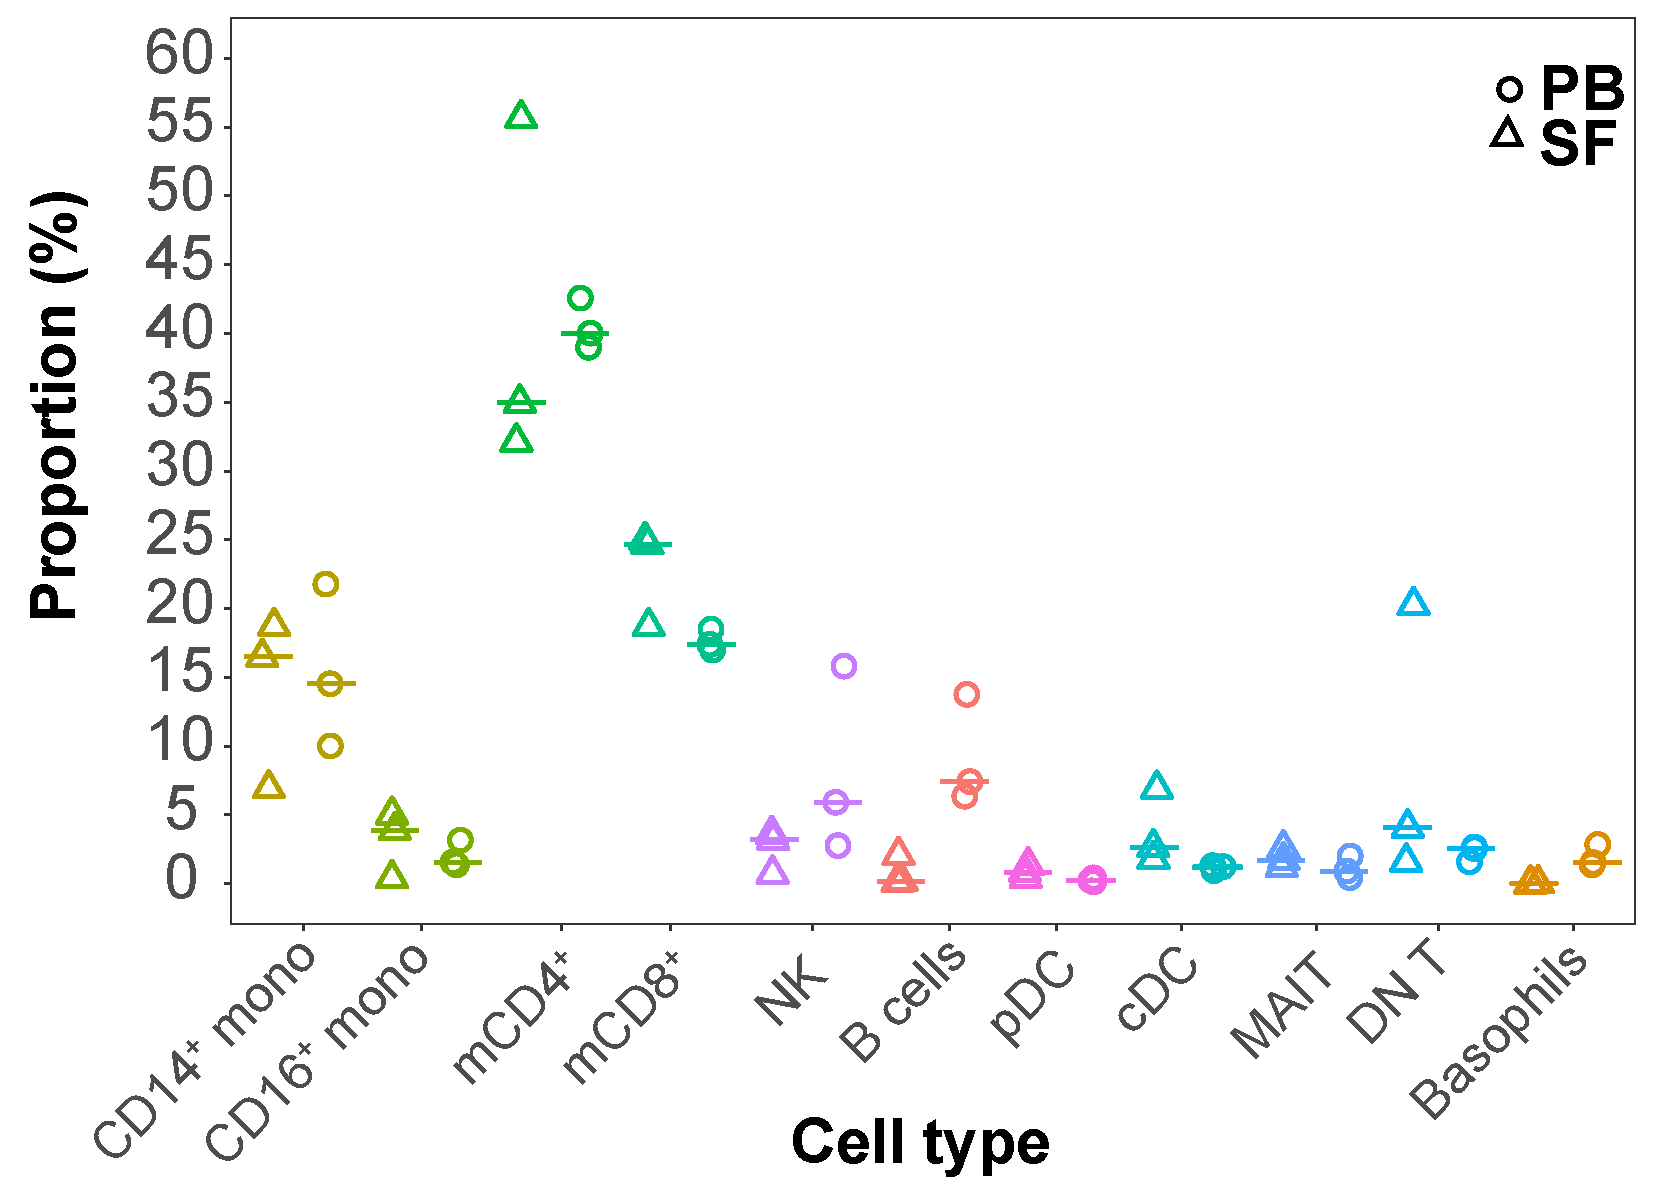
\includegraphics[width=0.7\textwidth]{./Results3/pdfs/PSA_ATAC_cohort_cell_type_composition_boxplots}
\caption[Comparative percentages of peripheral blood and synovial fluid immune cellular composition from the PsA cohort.]{\textbf{Comparative percentages of peripheral blood and synovial fluid immune cellular composition from the PsA cohort.} Percentages of each of the twelve cell types identified by mass cytometry are shown by individual and tissue for PsA1718, PsA1719 and PsA1607. Horizontal line represents the median percentage for a particular cell type in the appropriate tissue (synovial fluid or peripheral blood). Each of the cell types is displayed in a different colour. cDC=central DC; MAIT=mucosal-associated invariant T; DN=double negative; SF=synovial fluid; PB=peripheral blood.)}
\label{figure:PsA_cell_composition}
\end{figure}



\subsection{Differential chromatin accessibility analysis in immune cells reveals differences between synovial fluid and peripheral blood}


\subsubsection{Data processing and quality control}
Chromatin accessibility was studied in the four most abundant cell types in PsA synovium fluid, CD14$^+$ monocytes, mCD4$^+$, mCD8$^+$ and NK cells. The 24 ATAC samples (generated using Fast-ATAC protocol as detailed in Chapter \ref{ch:Mat}) from four cell types were sequenced and processes using the in-house pipeline as previously detailed (Chapters \ref{ch:Mat} and \ref{ch:Results1}). After filtering of duplicated and mitochondrial reads (Figure \ref{figure:PsA_FAST_ATAC_QC_supplementary}A), the median total number of reads was between 46.6 and 70.2 millions (Figure \ref{figure:PsA_FAST_ATAC_QC}A), depending on cell type (Figure \ref{figure:PsA_FAST_ATAC_QC}A). %The final number of reads remaining after filtering was inversely related to the percentage of MT and duplicated reads identified. For example, mCD14$^+$ and mCD8$^+$ presented the lowest median of total number of reads after filtering concomitantly with the greatest percentage of combined MT and duplicated reads. 
%As previously mentioned, the MT DNA in ATAC-seq is one of the main sources of read loss, which is more accessible to the Tn5 transposase due to the absence of nucleosomes. Although the FAST-ATAC protocol represented an improvement, the percentage of MT reads across amongst all the samples ranged between 2.1 and 25.4\%. Similarly, despite initial optimisation of the number of PCR cycles used in the library amplification, the duplicated reads still represented between 22.9 to 55\% of the total number sequenced reads.

TSS enrichment analysis showed differences in the levels of background noise across cell types and highlighted the variability of ATAC performance (Figure \ref{figure:PsA_FAST_ATAC_QC}B), where mCD4$^+$ and mCD8$^+$ showed the best signal-to-noise ratios. In contrast, NK was the cell type with the lowest TSS enrichment values with fold enrichments for PsA1719 and PsA1607 close to the 6 (ENCODE threhold cut-off). Given the limited cohort size, these samples were not excluded, but it is worth noting that they could be contributing noise and thus reducing the power of the differential analysis. The number of accessible regions (peaks after filtering with p-values based on IDR analysis) ranged between 24x10$^3$ and 97x10$^3$ (Figure \ref{figure:PsA_FAST_ATAC_QC_supplementary}B), and was also dependent of sample quality and cell type and no outliers were identified.

A combined consensus list of called ATAC peaks across all the samples and cell types (named here as CP\_all) was built (as previously explained in Chapters \ref{ch:Mat} \ref{ch:Results1}) and PCA was conducted on the normalised counts mapping to each of those peaks.

 

\begin{figure}[H]
\centering
\begin{subfigure}[b]{0.48\textwidth}
\centering 
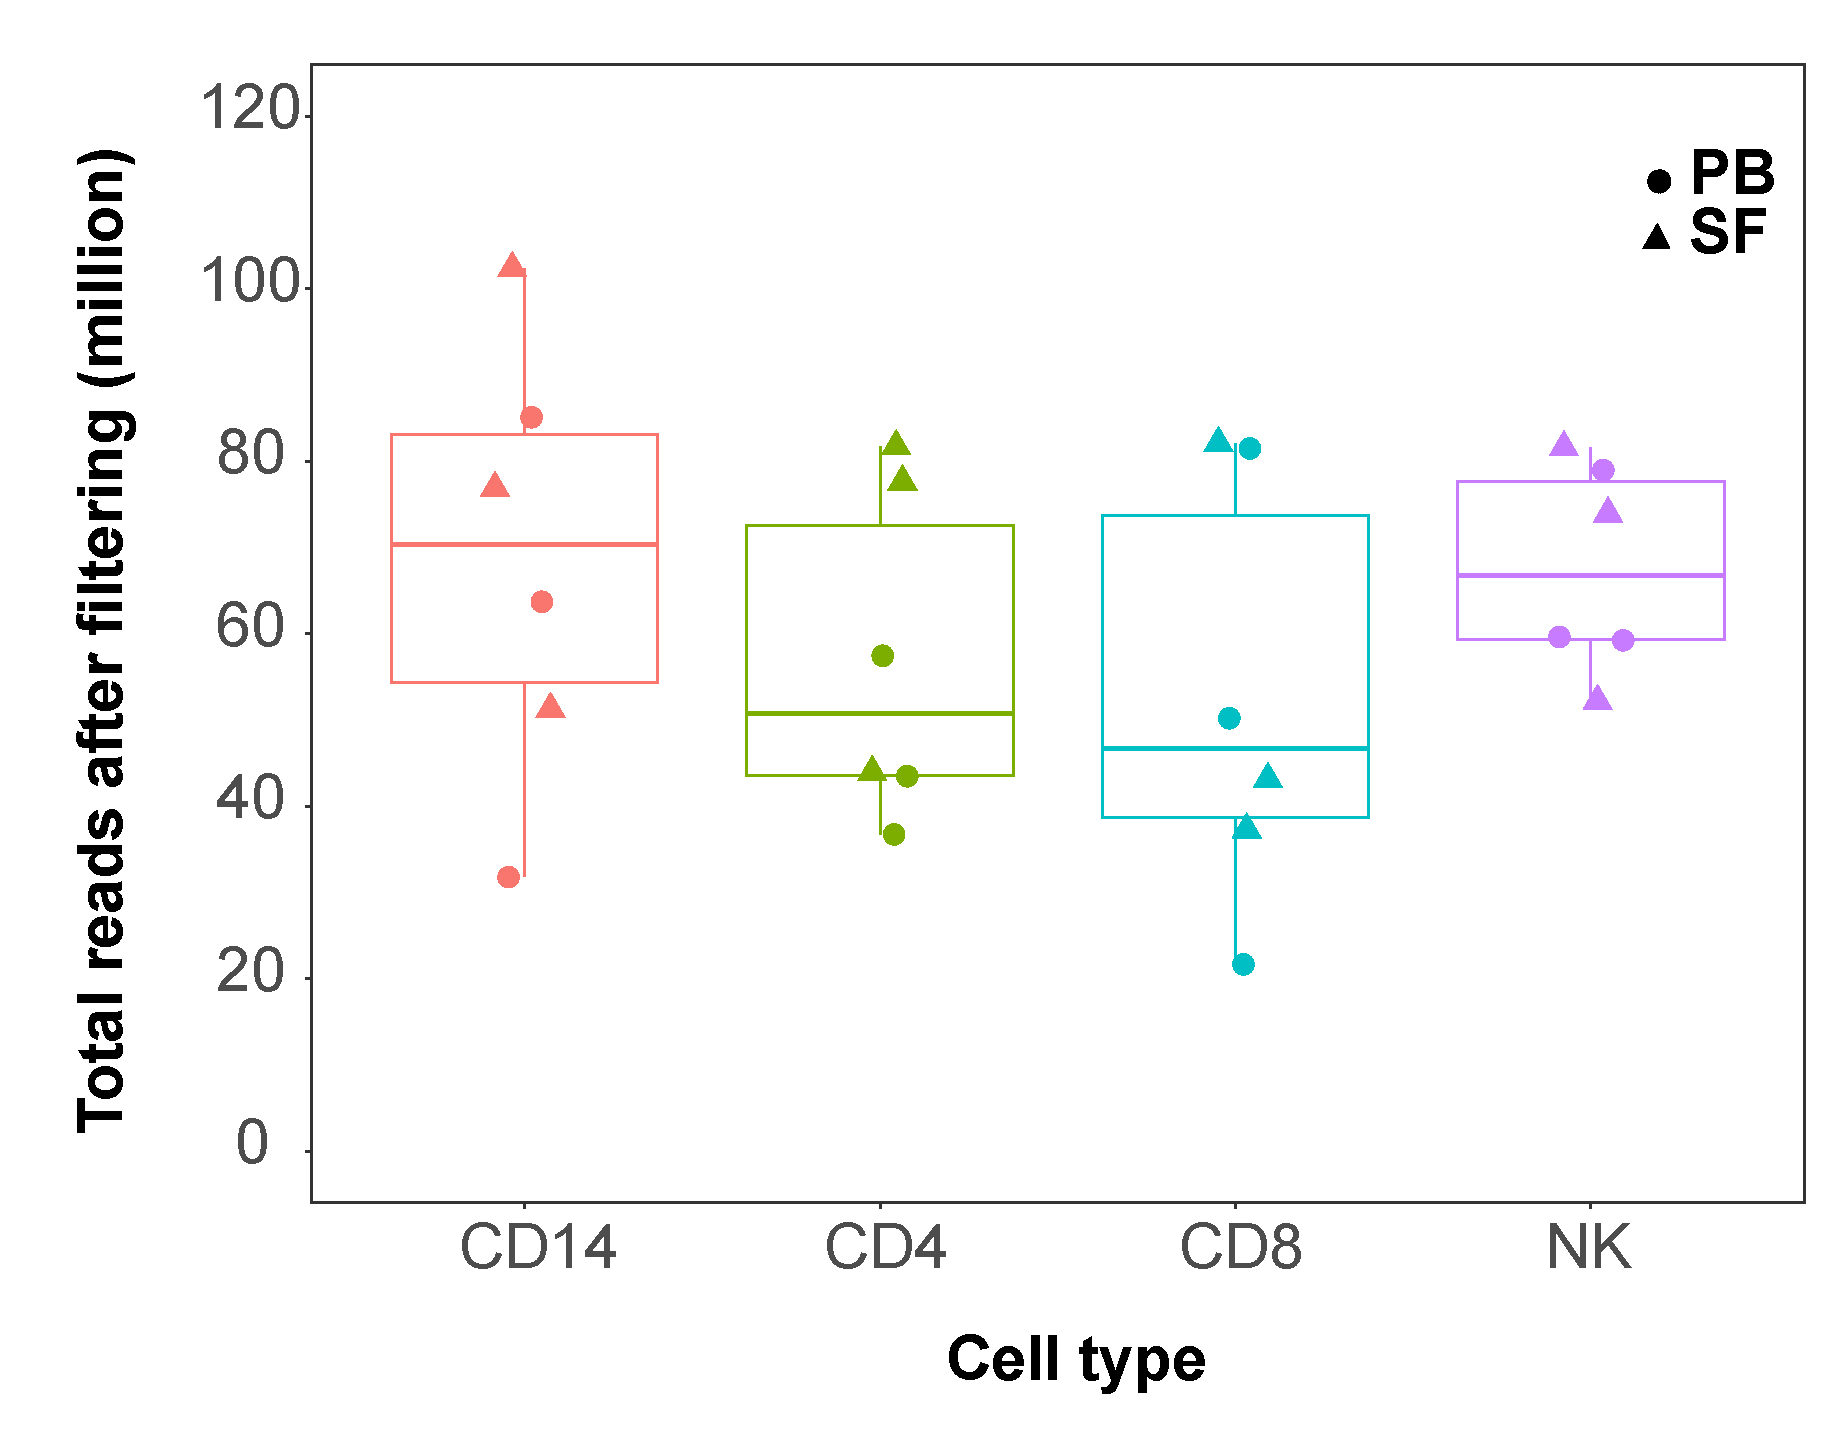
\includegraphics[width=\textwidth]{./Results3/pdfs/ATAC_PSA_total_filtered_reads_boxplot}
\caption{}
\end{subfigure}%
~
\begin{subfigure}[b]{0.48\textwidth} 
%the [b] prevents offset in subcaptions
\centering
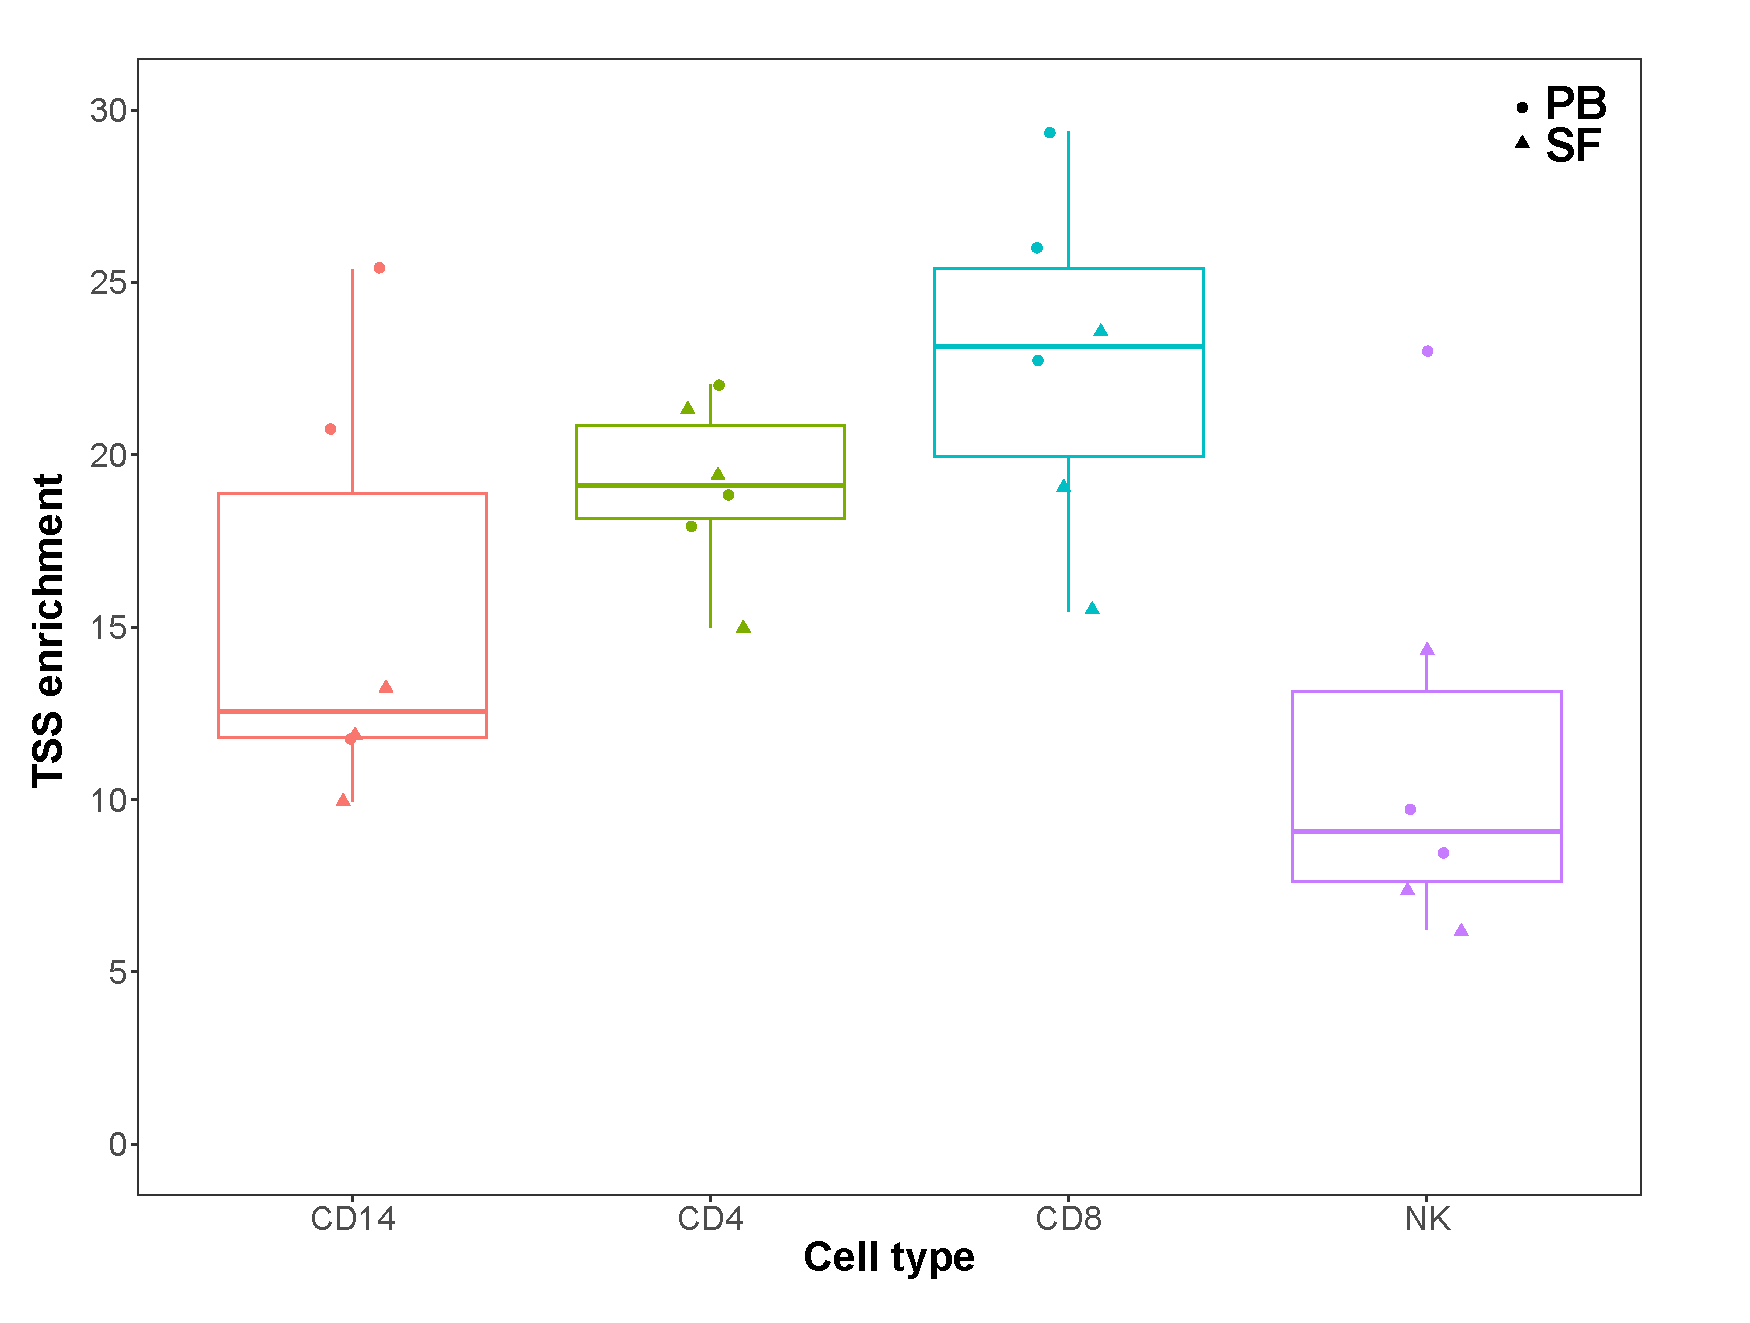
\includegraphics[width=\textwidth]{./Results3/pdfs/ATAC_PSA_all_TSS_max_per_cell_type}%
\caption{}
\end{subfigure}
\caption[Quality control assessment of ATAC data generated in four immune cell types isolated from peripheral blood and synovial fluid of PsA patients samples.]{\textbf{Quality control assessment of ATAC data generated in four immune cell types isolated from peripheral blood and synovial fluid of PsA patients samples.} For each of the cell types and samples, boxplots representing (A) million of reads after filtering and (B) values for fold-enrichment of ATAC fragments across the Ensembl annotated TSS. For each point, colour codes for cell type and shape for tissue (SF=synovial fluid; PB=peripheral blood).}
\label{figure:PsA_FAST_ATAC_QC}
\end{figure}



%For example, CD14$^+$ was the cell type with greatest number of called peaks (108.4$x10^3$) as well as the greater median of reads remaining after filtering when compared to the other three cell types (Figure \ref{figure:PsA_FAST_ATAC_QC} a). 
%For example, the two NK samples with the greatest TSS enrichment (PSA1718 synovial fluid and PB) showed larger number of called peaks when compared to the other NK samples with similar number of reads but lower quality measured by TSS enrichment. This observation was consistent with the correlation between sample quality and the number of identified accessible chromatin regions previously demonstrated in Chapter \ref{ch:Results1}. 
In this analysis, 65\% of the variability (PC1) in the chromatin landscape correlated with cell type, leading to sample separation into 4 clusters (Figure \ref{figure:PsA_FAST_ATAC_PCA}), demonstrating the ability to capture cell-type specific global differences in the regulatory landscape. The myeloid (CD14$^+$ monocytes) and lymphoid (mCD4$^+$ and mCD8$^+$) clusters were most distinct based on the ATAC profile, consistent with biological expectations. Modest separation between synovial fluid and peripheral blood samples was also observed in mCD8$^+$ and NK cells clusters (Figure \ref{figure:PsA_FAST_ATAC_PCA}).



\begin{figure}[htbp]
\centering
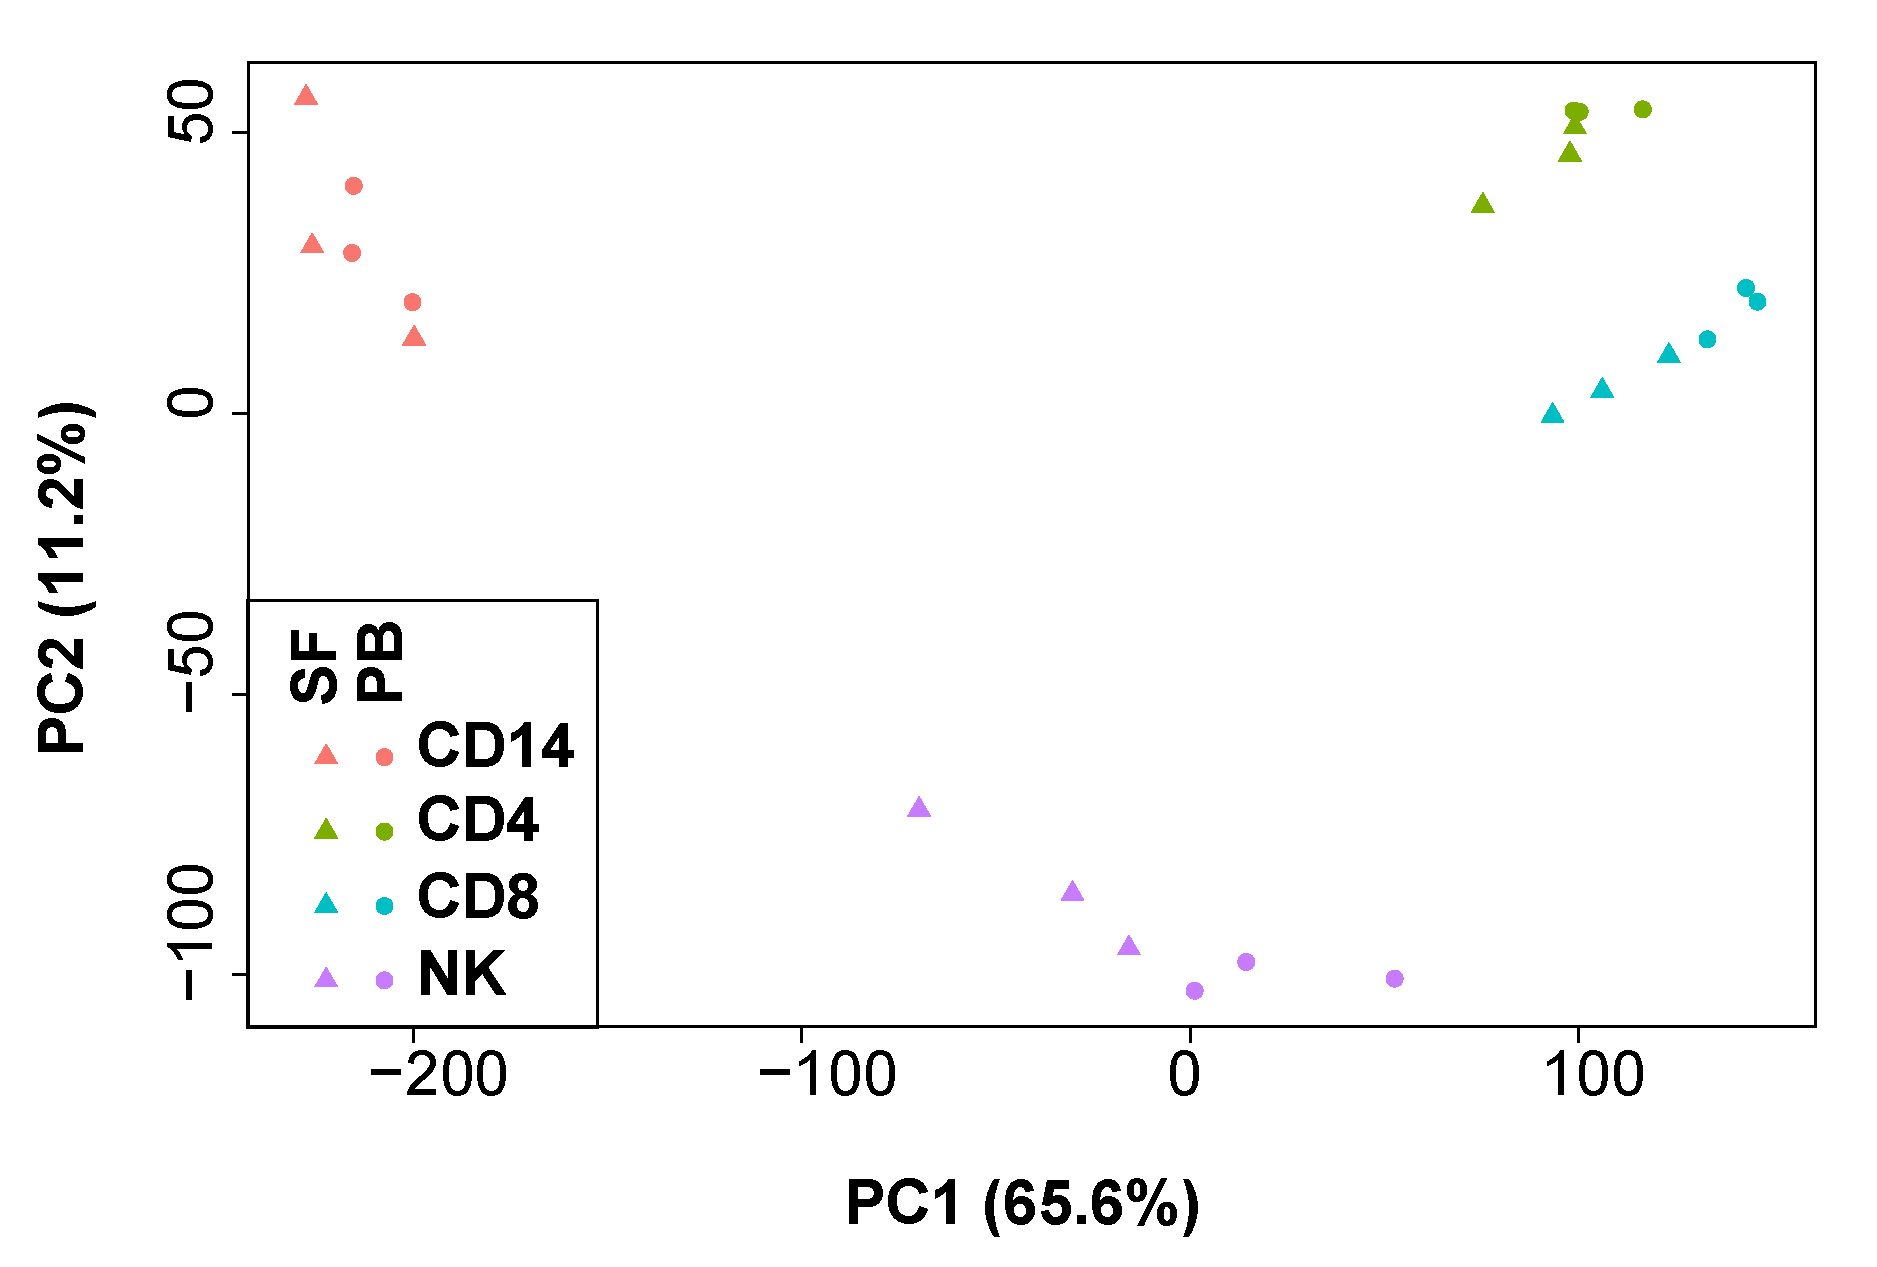
\includegraphics[width=0.65\textwidth]{./Results3/pdfs/ATAC_PSA_all_DESEq2_PCA}
\caption[PCA based on the ATAC chromatin accessibility landscape in four immune cell types isolated from blood and synovial fluid.]{\textbf{PCA based on the ATAC chromatin accessibility landscape in four immune cell types isolated from blood and SF.} The analysis was performed using the normalised counts mapping to each of the peaks included in the consensus list of called peaks (CP\_all) across all four cell types (CD14$^+$ monocytes, mCD4$^+$, mCD8$^+$ and NK cells) and two tissues of interest (total of 24 samples). The first two PCs (x-axis and y-axis, respectively) for the ATAC peaks included in the ML\_all are plotted. Each point represents a sample, where colour indicates cell type and shape tissue (SF=synovial fluid; PB=peripheral blood). The proportion of variation explained by each principal component is indicated.}
\label{figure:PsA_FAST_ATAC_PCA}
\end{figure}



%The ability to capture putative regulatory regions within the identified accessible chromatin regions was also explored. Enrichment analysis of different eQTL publicly available datasets for the regions contained in the MASTER\_ALL list was performed. Amongst the GTEx eQTL data, the largest (z-score) and most significant (-log$_10$FDR) enrichment was found for the venous blood data set (red dot), consistent with the cell types included in the study (Figure \ref{figure:PsA_FAST_ATAC_eQTL_enrichment} a). In terms of publicly available eQTLs studies in immune cells, the strongest enrichment for the MASTER\_ALL regions were found for CD14$^+$ monocytes (importantly unstimulated, LPS 2h and IFN-$\gamma$ 24h) followed by mCD8$^+$ T cells (Figure \ref{figure:PsA_FAST_ATAC_eQTL_enrichment} b). eQTLs in B cell appeared as the least enriched when compared to the other datasets, consistently with the absence of this cell type in the ATAC experiments, and reinforcing the cell specificity captured by this assay.

%\bigskip
%\begin{figure}[H]
%\centering
%\begin{subfigure}[b]{0.5\textwidth}
%\centering 
%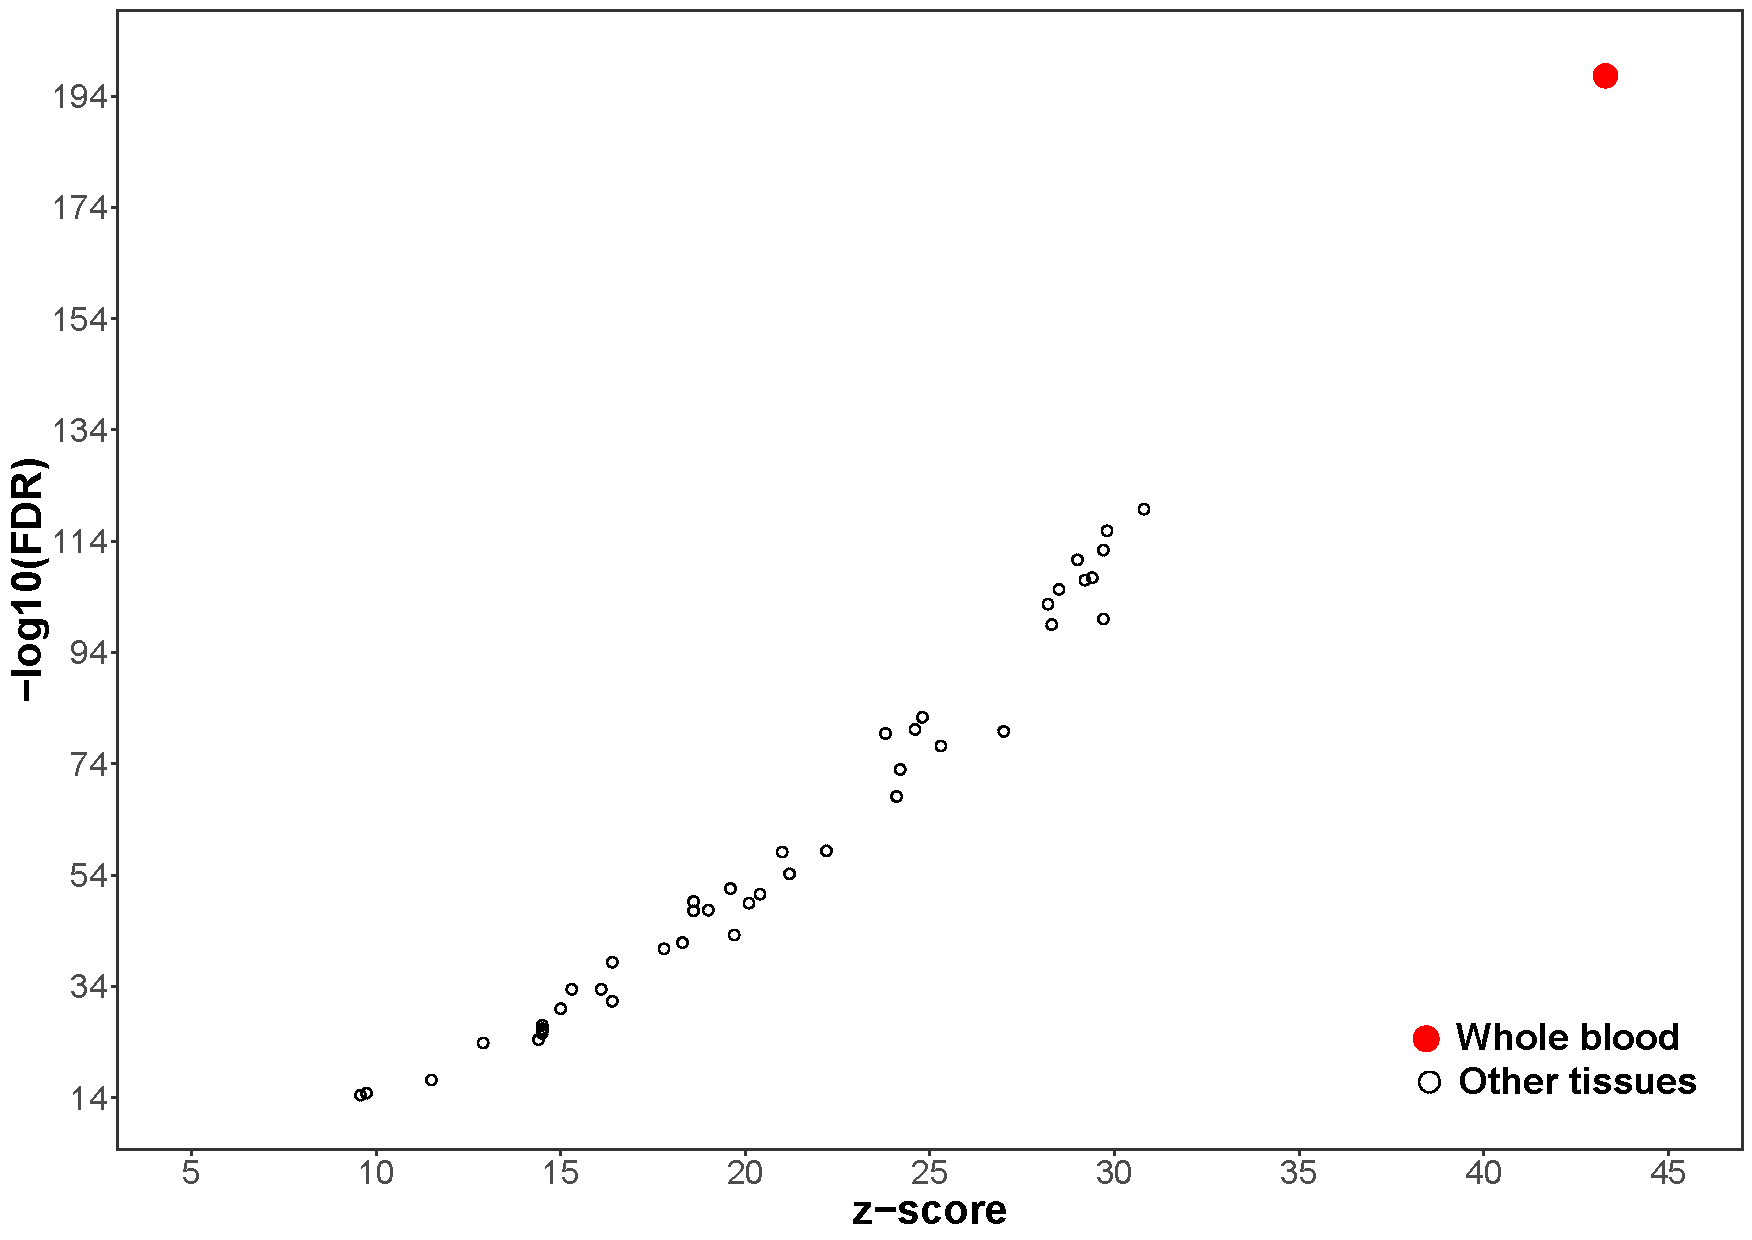
\includegraphics[width=\textwidth]{./Results3/pdfs/ATAC_PSA_all_GTeX_eQTL_enrichment_dotplot}
%\caption{}
%\end{subfigure}%
%\begin{subfigure}[b]{0.5\textwidth} 
%%the [b] prevents offset in subcaptions
%\centering
%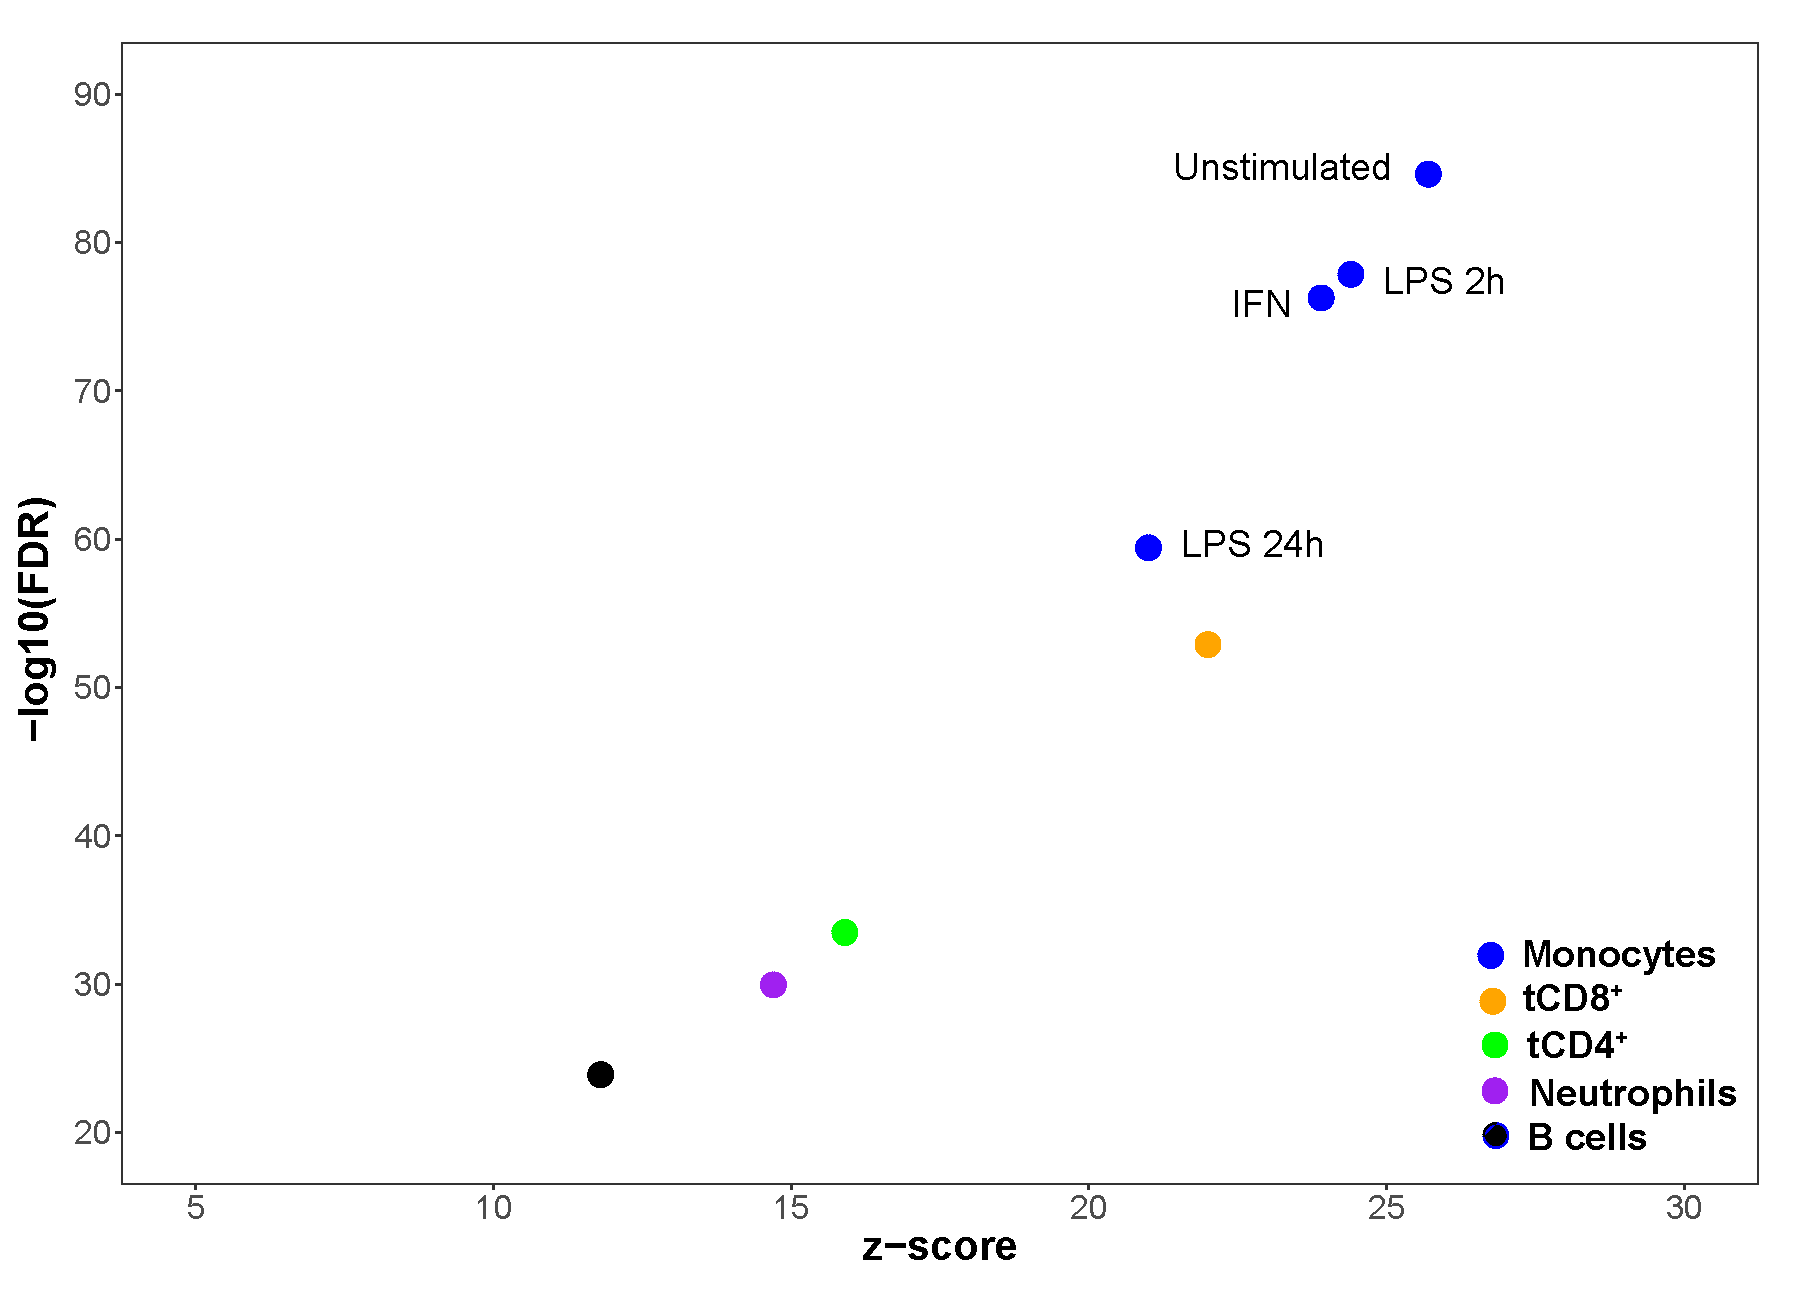
\includegraphics[width=\textwidth]{./Results3/pdfs/ATAC_PSA_all_Jknight_eQTL_enrichment_dotplot}
%\caption{}
%\end{subfigure}
%\caption[Enrichment of eQTLs publicly available data in the combined cell type and tissue chromatin accessibility master list for the PsA cohort.]{\textbf{Enrichment of eQTLs publicly available data in the combined cell type and tissue chromatin accessibility master list for the PsA cohort.} The dot plots showed the z-score values of the enrichment analysis in the x-axis and the significance (-log${_10}$FDR) in the y-axis for (A) GTEx eQTL datasets and (B)non-GTEx immune-related cell types including CD14$^+$ monocytes (unstimulated, LPS 2h, LPS 24h and 24h IFN$\gamma$ stimulated), B cells, tCD4$^+$, tCD8$^+$ and neutrophils. Dots are colour-coded by cell type.}
%\label{figure:PsA_FAST_ATAC_eQTL_enrichment}
%\end{figure}



\subsubsection{Characterisation of the differential accessible regions between synovial fluid and peripheral blood}

In order to perform differential chromatin accessibility analysis between synovial fluid and peripheral blood, a consensus list of ATAC peaks (accessible chromatin regions) was built for each cell types (named here as CP\_CD14, CP\_mCD4, CP\_mCD8, and CP\_NK) (detailed in Chapter \ref{ch:Mat}). %\ToDo{Regions included in each consensus list of peaks were enriched for SNPs from the GTEx eQTL datasets, importantly whole blood, as well as for immune cells eQTL SNPs from publicly available data (Figure \ref{figure:eQTL_enrichment_CP_all_cell_types}), demonstrating the inclusion of functionally relevant regions in the downstream differential analysis.}
 Differential chromatin accessibility analysis between synovial fluid and peripheral blood using normalised counts retrieved for each of the cell type master lists using DESeq2 with a paired design (Table \ref{tab:PSA_DOCs_results}). Using an 80\% cut-off for background noise (Chapter \ref{ch:Results1}), %Only differentially accessible regions (DARs) identified with DESeq2 and also shared with quantile normalisation limma voom analysis where considered downstream. 
CD14$^+$ monocytes and NK cells showed the greatest total number (5,285 and 2,314, respectively) and proportion of DARs (9.1 and 8.9\%, respectively). 


\begin{table}[htbp]
%\setlength{\tabcolsep}{20pt} only to stretch the columns if you want
%\renewcommand{\arraystretch}{1.5}
\centering
\begin{tabular}{@{}c c c c c}
\toprule
\textbf{Cell type}  & \textbf{Total DARs} &  \textbf{Proportion}  & \textbf{Synovial fluid } & \textbf{Peripheral blood} \\
                    &                     &  \textbf{DARs (\%)}  & \textbf{open DARs} & \textbf{open DARs} \\
\midrule
\midrule
CD14$^+$ & 5,285 & 9.1 & 3,779 & 1,506 \\
CD4$^+$  & 1,329 & 4.3 & 621 & 708 \\
CD8$^+$  & 1,570 & 4.5 & 807 & 763 \\
NK       & 2,314 & 8.9 & 1,223 & 1,091 \\
\bottomrule
\end{tabular}
\medskip %gap
\caption[Summary results of the differential chromatin accessibility analysis between synovial fluid and peripheral blood in PsA samples.]{\textbf{Summary results of the differential chromatin accessibility analysis between synovial fluid and peripheral blood in PsA samples.} For each of the cell types the total number of DARs and the proportion represented by DARs over all the regions included in the differential analysis are reported. The total number of DARs are further divided in those more accessible in synovial fluid (synovial fluid open DARs) when compared to peripheral blood and those less accessible in synovial fluid when compared to peripheral blood (peripheral blood open DARs).}
\label{tab:PSA_DOCs_results}
\end{table}

Considering the direction of the differential chromatin accessibility, DARs were divided in DARs more open in synovial fluid compared to peripheral blood (named here synovial fluid open DARs) and DARs less open in synovial fluid compared to peripheral blood (named here peripheral blood open DARs). In CD14$^+$ monocytes the number of synovial fluid open DARS were notably larger than the number of peripheral blood open DARs (3,779 and 1,506 DARs, respectively) (Table \ref{tab:PSA_DOCs_results}). In contrast, a similar proportion of synovial fluid and peripheral blood open DARs were found for the other three cell types.

Permutation analysis using the unique ten possible permutations (given the small number of samples included in the analysis) did not show a greater number of DARs than the ones identified for the true groups, reinforcing the robustness of the differential analysis results (Figure \ref{figure:PsA_perm_analysis}).


%Permutation analysis was used to determine if the large number of DARs (particularly by comparison to limited finding in the psoriasis analysis) were more than would be expected by chance. None of the unique 10 possible permutations (given the small number of samples included in the analysis) demonstrated a greater number of DARs than the ones identified for the true groups, reinforcing the robustness of the differential analysis results (Figure \ref{figure:PsA_perm_analysis}).

  
Genomic annotation of the DARs identified in each the cell types revealed that 80\% or more of all regions with differential accessibility were located at intronic and intergenic regions (Figure \ref{figure:PsA_FAST_ATAC_DOCS_annotation}A). 

\bigskip
\begin{figure}[htbp]
\centering
\begin{subfigure}[b]{0.7\textwidth}
\centering 
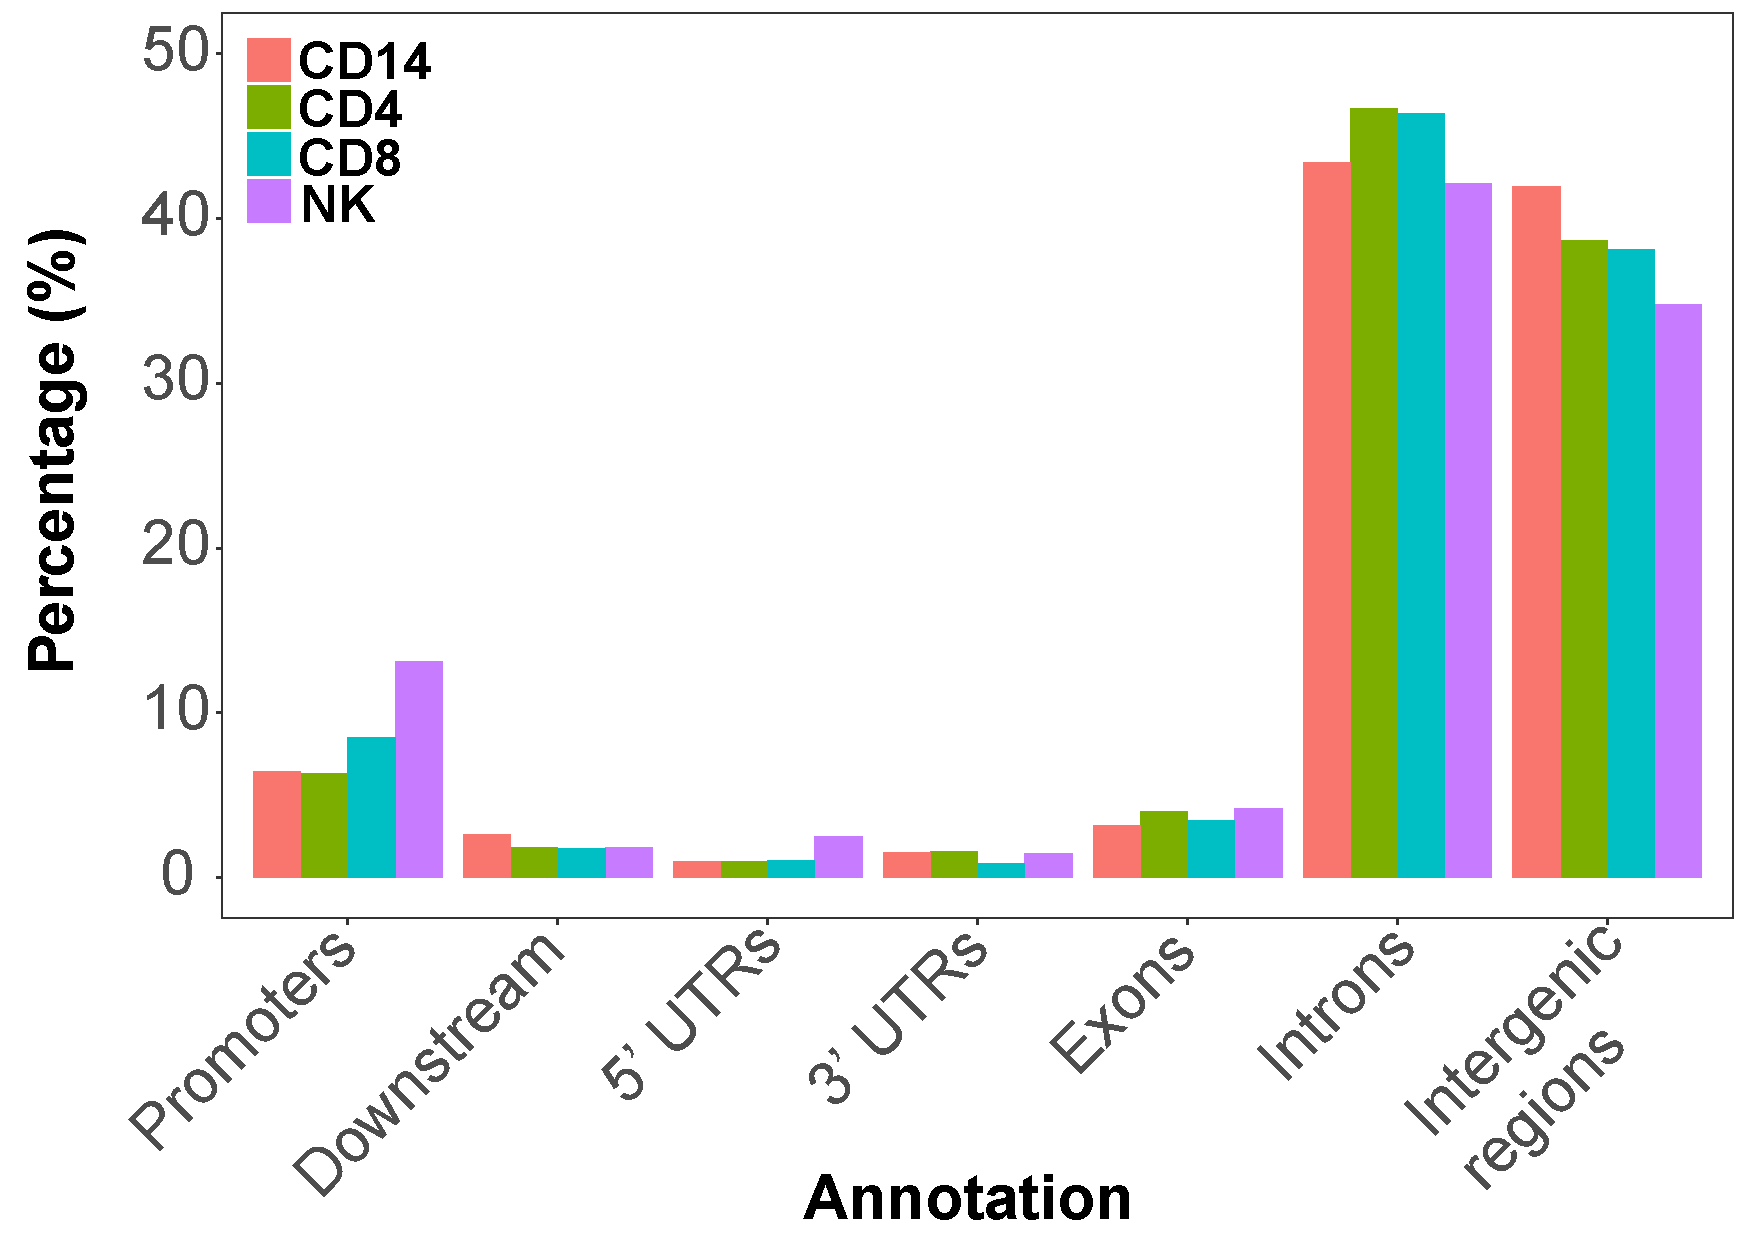
\includegraphics[width=\textwidth]{./Results3/pdfs/ATAC_PSA_DOCS_per_cell_type_general_annotation}
\caption{}
\end{subfigure}
~
\begin{subfigure}[b]{0.75\textwidth} 
%the [b] prevents offset in subcaptions
\centering
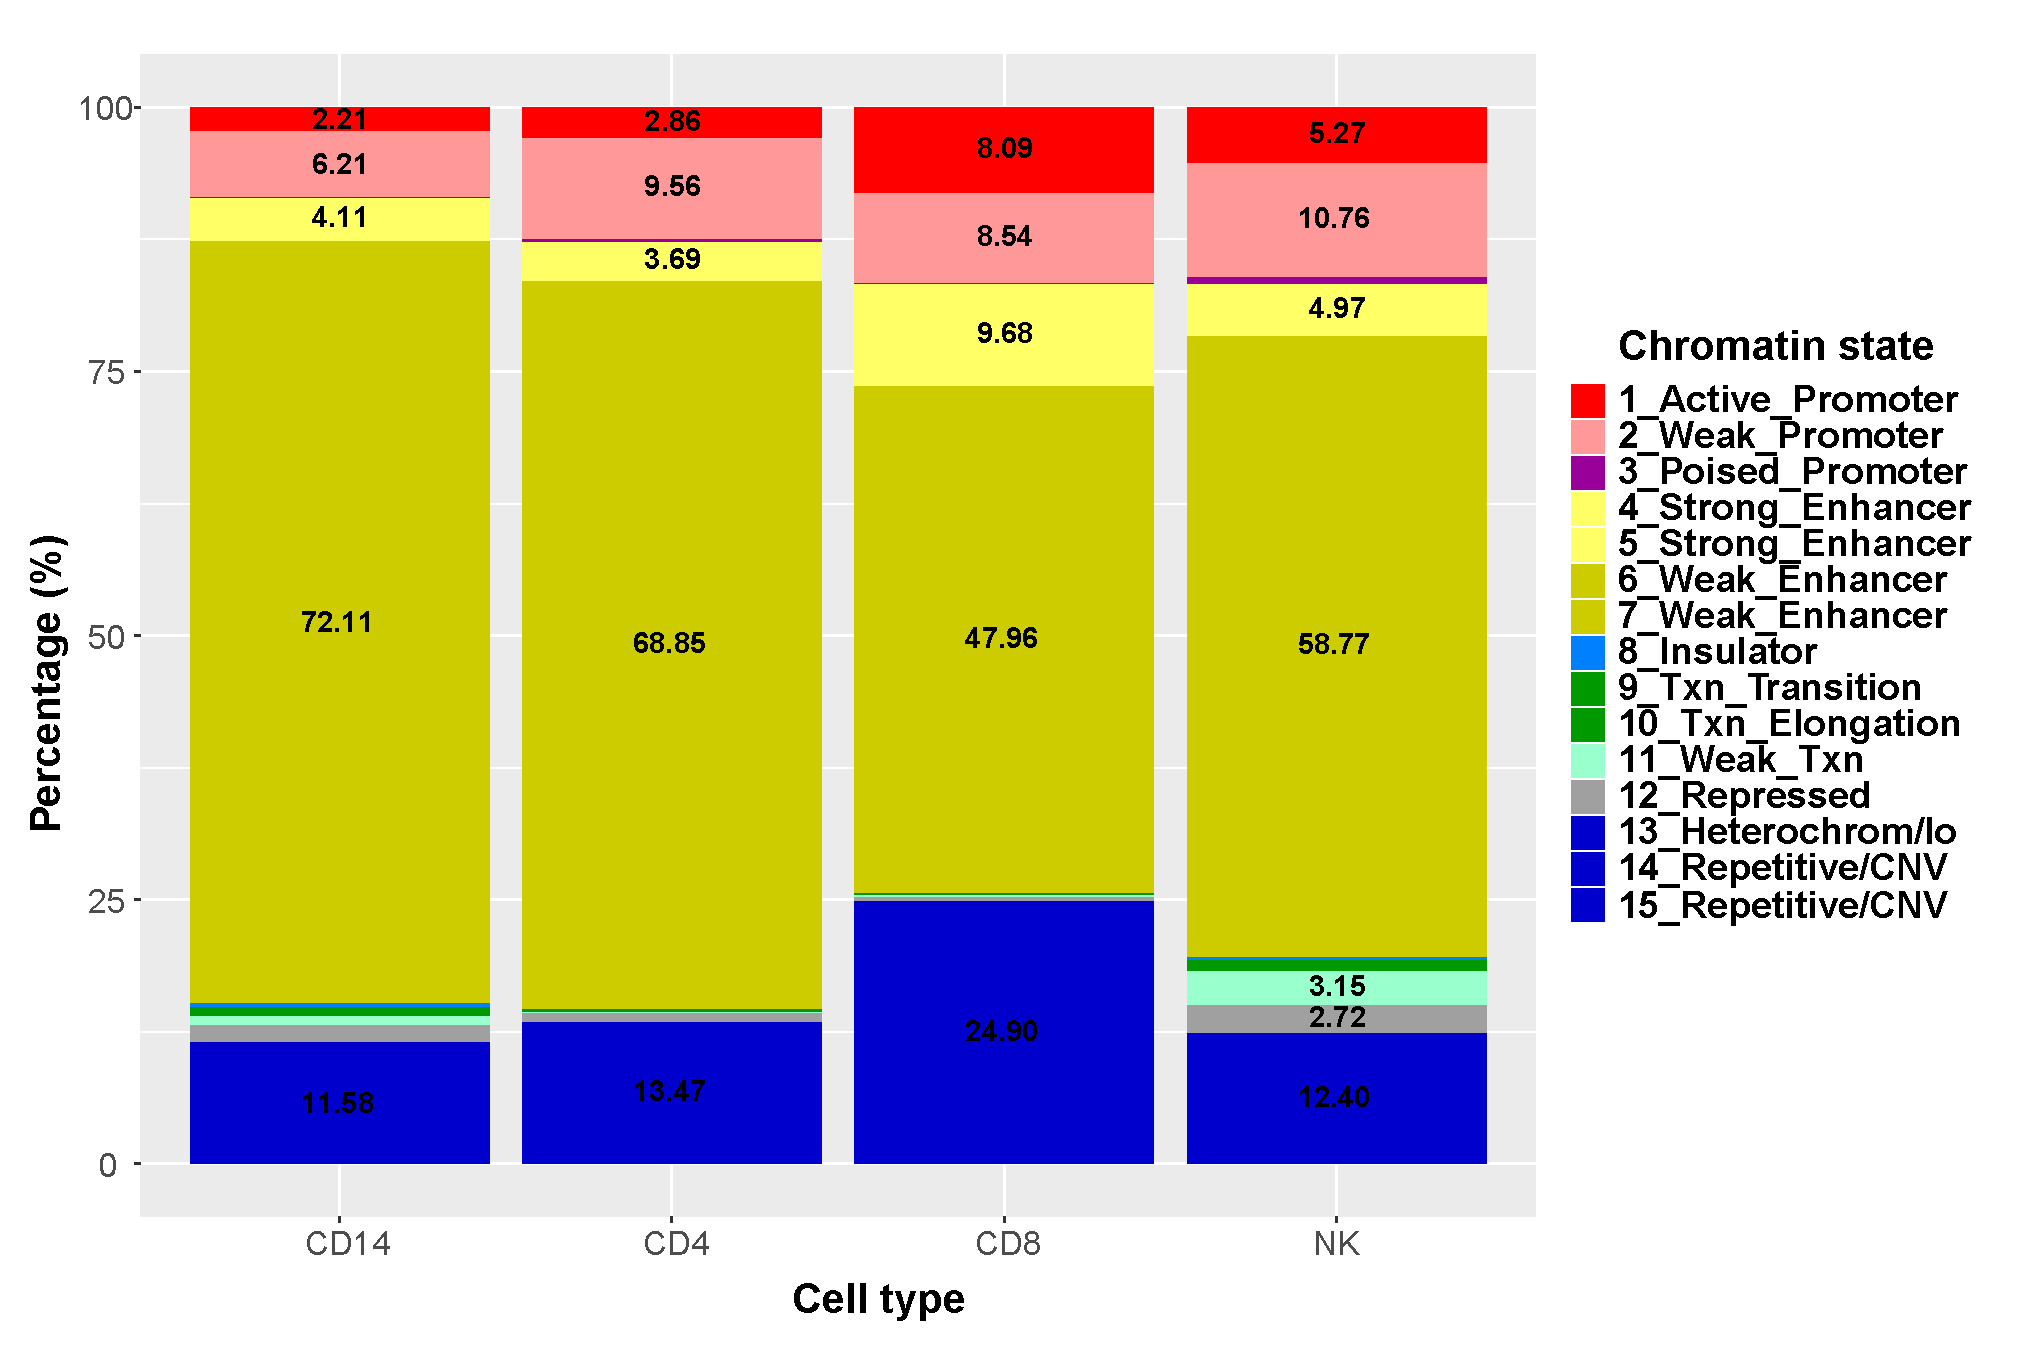
\includegraphics[width=\textwidth]{./Results3/pdfs/ATAC_PSA_DOCS_chromatin_states_stacked_barplot}
\caption{}
\end{subfigure}
\caption[Annotation of the PsA DARs identified in the four cell types with genomic annotations and chromatin states.]{\textbf{Annotation of the PsA DARs identified in the four cell types with genomic annotations and chromatin states.} (A) Barplot illustrating the percentage of nucleotides within DARs for each cell type that are annotated as promoters, downstream (regions at $\leq$1,000bp to a promoter), exons, introns, 5' or 3'UTR and intergenic regions. (B) Stacked barplot representing the percentage of DARs annotated for each of the 15 chromatin states defined in each of the four relevant cell types by Roadmap Epigenomics Project chromatin segmentation maps (CD14$^+$ peripheral blood isolated monocytes, mCD4$^+$, mCD8$^+$ and NK cells).}
\label{figure:PsA_FAST_ATAC_DOCS_annotation}
\end{figure}

Universal promoter regions were the third most represented genomic feature, accounting for the annotation of approximately 5 to 15\% of the DARs in each cell type (Figure \ref{figure:PsA_FAST_ATAC_DOCS_annotation}A). For all four cell types, between 44.96 and 72.11\% of the DARs were annotated as enhancers based on cell-type specific chromatin segmentations maps, the category accounting for the largest proportion of DARs and the most significantly enriched (Figures \ref{figure:PSA_ATAC_DARs_chromatin_states_enrichment} and \ref{figure:PsA_FAST_ATAC_DOCS_annotation}). The over-representation of enhancers was consistent with large percentage of introns and intergenic regions found for the genomic features annotation, as those are the preferred location for enhancer elements. Modest percentages of DARs were also annotated as heterochromatin and repetitive regions, which partly represent intrinsic technical noise but could also reflect specific synovial fluid features that have not been captured by the chromatin segmentation maps generated using peripheral blood immune cells.
%
%Try to overlap the enhancer FANTOM data to id those regions whith evidence of eRNA expression
The functional relevance of the differential chromatin accessibility in terms of regulation of gene expression was further investigated by integration of the eRNA data from the FANTOM5 project. Statistically significant enrichment for robust and permissive enhancers was found for the DARs in all four cell types (Figure \ref{figure:PSA_FANTOM}).  Moreover, DARs from all four cell types also showed significant enrichment for the corresponding cell type robust eRNA set. The proportion of DARs overlapping the appropriate cell type set of expressed eRNAs ranged between 198 (122 synovial fluid open and 76 peripheral blood open) in mCD4$^+$ T cells and 924 DARs (690 synovial fluid open and 234 open in peripheral blood) in CD14$^+$ monocytes.


\begin{figure}[htbp]
\centering
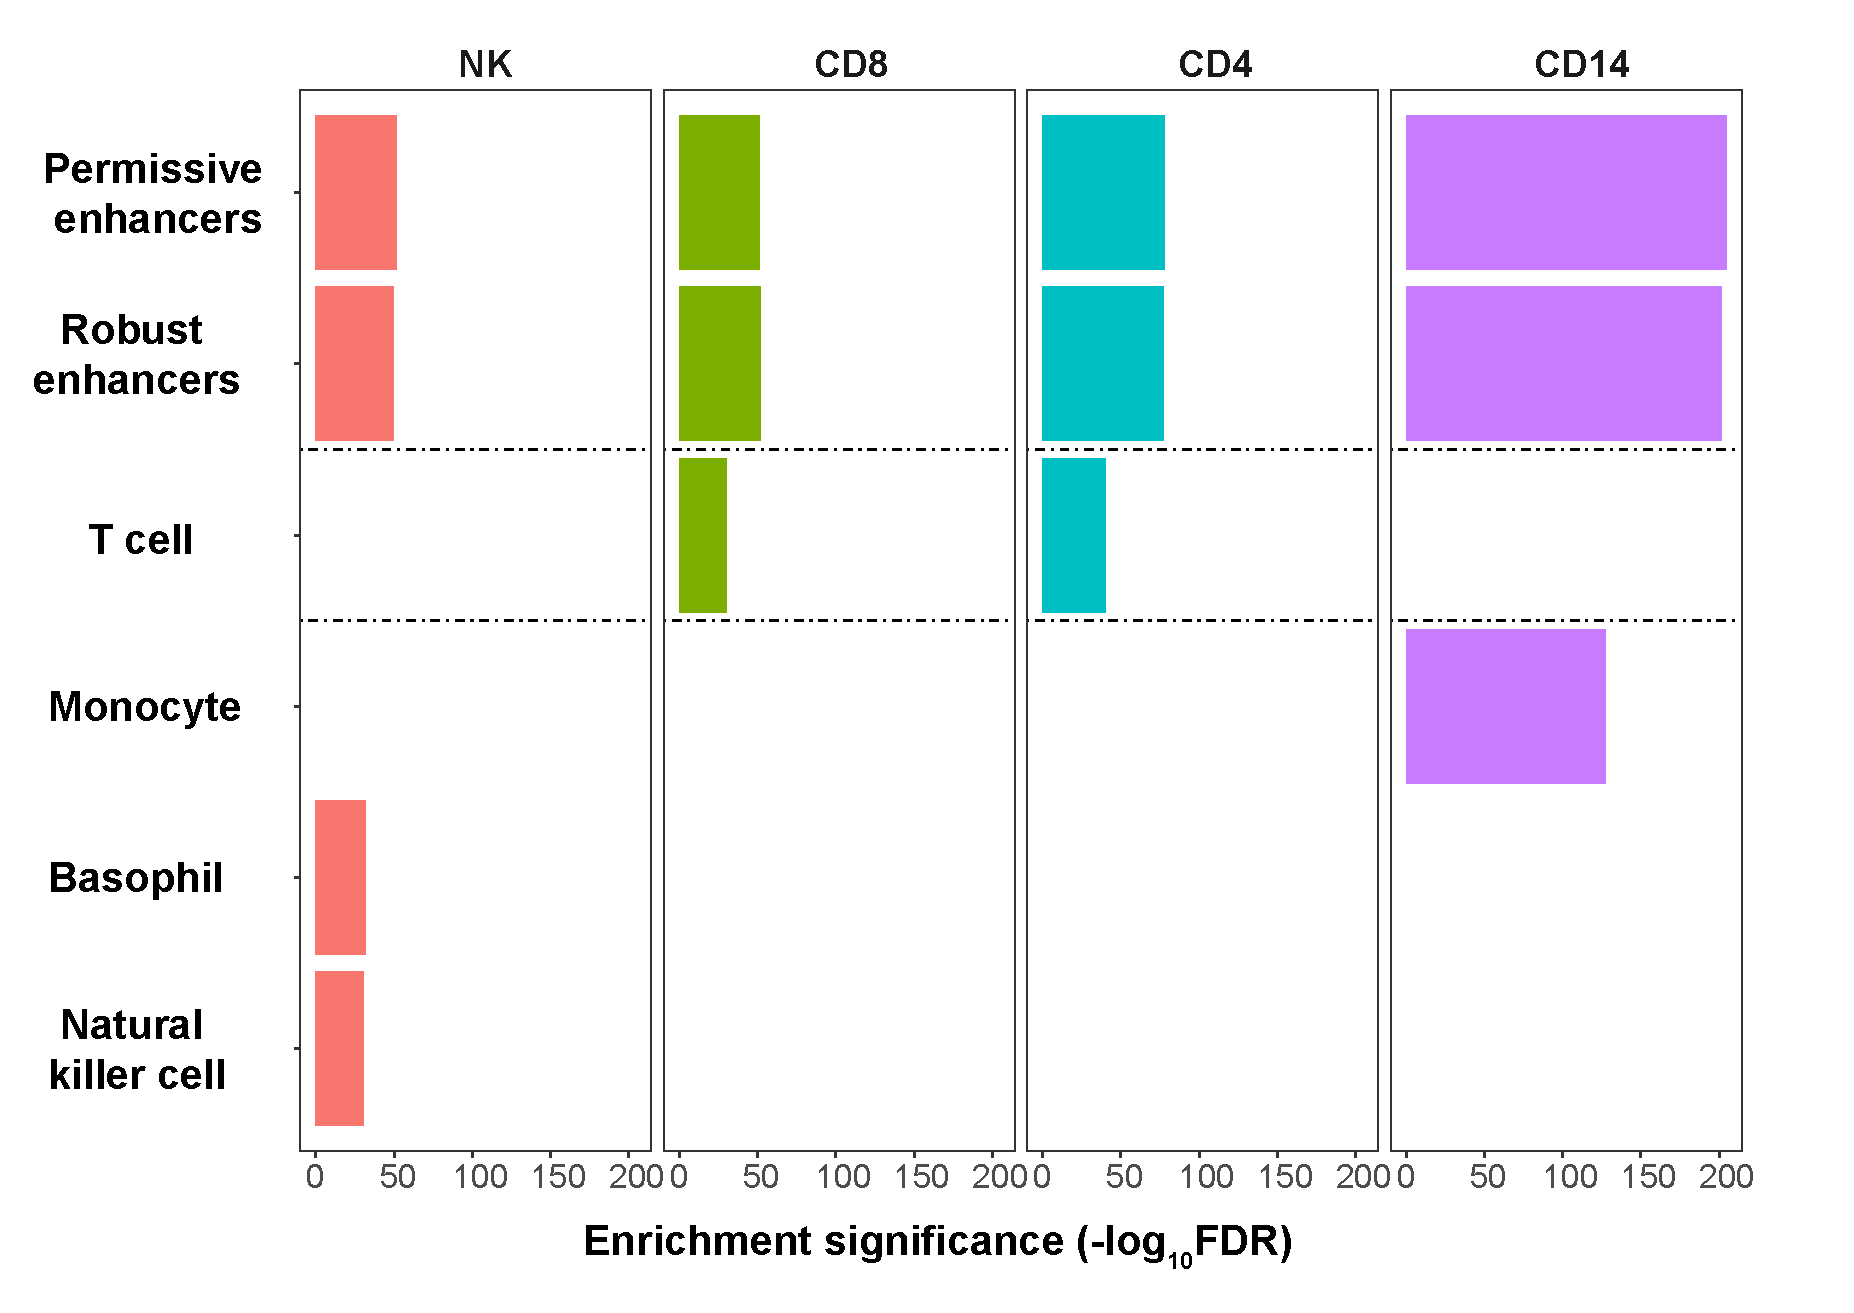
\includegraphics[width=0.6\textwidth]{./Results3/pdfs/ATAC_PsA_FANTOM_enhancer_enrichment_all_cell_types}
\caption[Enrichment of PsA DARs for the FANTOM5 eRNA dataset.]{\textbf{Enrichment of PsA DARs for the FANTOM5 eRNA dataset.} Robust enhancers have been defined as those detected at the genome-wide significant level in at least one primary cell type or tissue. Permissive enhancers are all detected eRNAs but not passing genome-wide filtering criteria \parencite{Andersson2014}. Robust enhancers represent a subset of the permissive enhancers. Total number of DARs overlapping a robust eRNA detected in the corresponding cell type are indicated. Significant enrichment is considered for FDR$<$0.01.}
\label{figure:PSA_FANTOM}
\end{figure}

The differential analysis demonstrated that a number of DARs were overlapping a gene body (Table \ref{tab:PSA_DOCs_gene_body}). Interestingly, the majority were located within introns instead of untranslated regions (UTRs) annotated as weak or strong enhancers according to the cell-type specific chromatin segmentation map previously illustrated. 

%Similarly, more accessible chromatin in synovial fluid compared to peripheral blood was identified in five regions of the \textit{IL15} gene, annotated as promoter and enhancers in CD14$^+$ monocytes. 
% Check differences at both gene locations were CD14$^+$ cell type specific is this region HiC annotated with the gene? and maybe include example overlapping eRNA
%e.g LMNA4 which is CD14 cell specific and more expressed in synovial fluid in Dolcino paper. Maybe use it later

\begin{table}[htbp]
%\setlength{\tabcolsep}{20pt} only to stretch the columns if you want
%\renewcommand{\arraystretch}{1.5}
\centering
\begin{tabular}{@{} c c c c c}
\toprule
\textbf{Cell type} & \textbf{DARs in} &  \textbf{Gene with more}     &\textbf{Enhancers} & \textbf{Introns} \\
                   & \textbf{gene body} &  \textbf{than one DAR} &                   &                   \\
\midrule
\midrule
CD14$^+$ & 2,357 & 744 & 1,775 & 1,920 \\
CD4$^+$ & 700 & 99 & 504 & 577 \\
CD8$^+$ & 831 & 118 & 503 & 666 \\
NK   & 1,246 & 235 & 782 & 937 \\   
\bottomrule
\end{tabular}
\medskip %gap
\caption[Characterisation of the DARs located within genes in each of the four cell types from PsA samples.]{\textbf{Characterisation of the DARs located within genes in each of the four cell types from PsA samples.} The number of DARs overlapping a gene body for each of the cell types are indicated together with those genes harbouring more than one DARs. Further details about those regions includes specification of the number located at introns and those annotated as enhancers according to the Roadmap Epigenomics Project chromatin segmentation maps of each appropriate cell type.}
\label{tab:PSA_DOCs_gene_body}
\end{table}

For example, differential chromatin accessibility analysis in NK cells identified a DAR located in an intron of the \textit{VAV3} gene that was also more accessible in peripheral blood compared to synovial fluid, and also significantly expressed as an eRNA (Figure \ref{figure:PsA_FAST_ATAC_gene_boy_DOCS_CD14_NK}A). By contrast, an example in CD14$^+$ monocytes of two DARs, located at the 5' and 3' UTRs of \textit{IL7R} gene, were more accessible in synovial fluid compared to peripheral blood (Figure \ref{figure:PsA_FAST_ATAC_gene_boy_DOCS_CD14_NK}B). 

% GWAS overlap maybe indicate an example in CD14 that can be relevant with pathway analysis
%The relevance of the differences in chromatin accessibility in the context of psoriasis and PsA GWAS hits was also addressed. Enrichment analysis of psoriasis and PsA GWAS hits for the DARs in each cell type was performed using XGR co-localisation and permutation analysis. At the SNP level, no significant enrichment was reported between DARs and GWAS lead SNPs and those in LD r$^2$$\geq$8. When the enrichment analysis was performed for the psoriasis and PsA LD blocks, significant enrichment (2-fold enrichment and empirical p-val 0.043) was observed only for the CD14$^+$ DARs.

Additionally, DARs in all four cell types were shown to overlap or be proximal ($\leq$5Kb) with genes nearby psoriasis and PsA GWAS loci. CD14$^+$ monocytes presented the largest number of overlaps (13), followed by mCD8$^+$ (9), NK$^+$ (8) and mCD4$^+$ (4). For example, DARs proximal to \textit{ELMO1} and \textit{RUNX3} were found for all the cell types. Moreover, LD-based enrichment analysis was conducted between psoriasis and PsA GWAS catalogue LD blocks and the DARs identified in each of the cell types. This analysis compared the observed to the expected overlap between a null distribution of LD blocks from all common SNPs, respecting allele frequencies and proximity to genes of the GWAS lead SNP of each block (see Chapter \ref{ch:Mat}). Significant enrichment of GWAS LD blocks for DARs between synovial fluid and peripheral blood in CD14$^+$ monocytes (empirical p-value=0.043) was observed using a total of 20,000 permutations.

\bigskip
\begin{figure}[H]
\centering
\begin{subfigure}[b]{0.60\textwidth}
\centering 
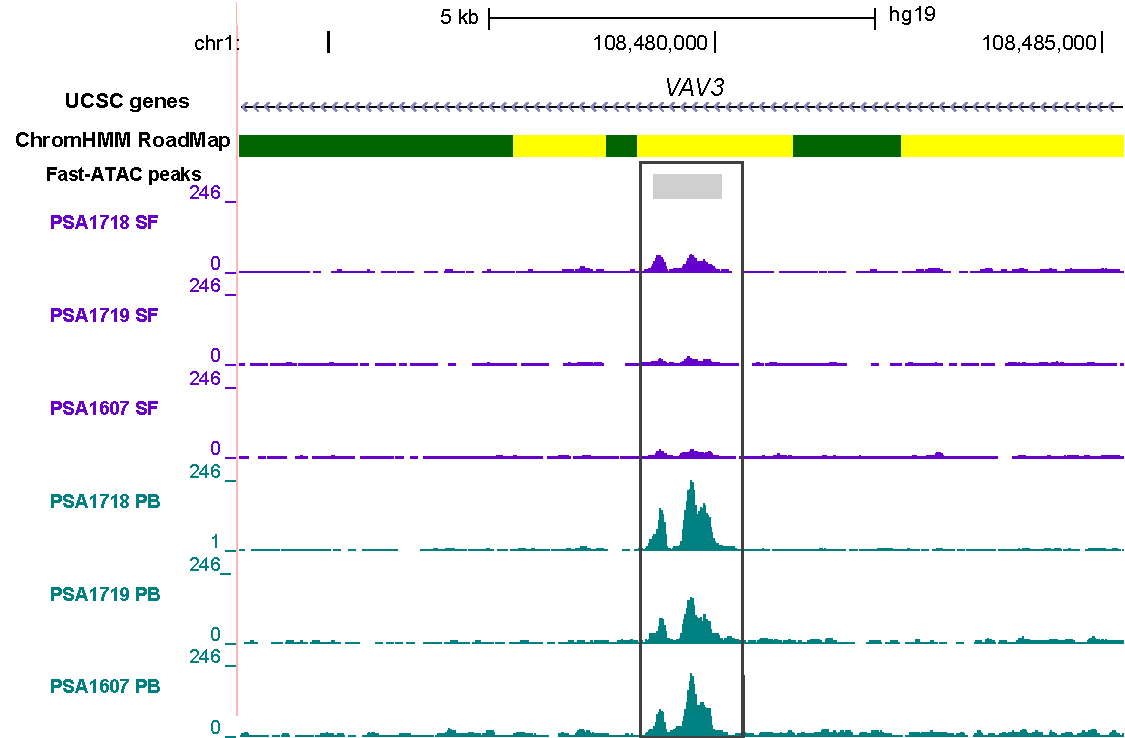
\includegraphics[width=\textwidth]{./Results3/pdfs/ATAC_PSA_NK_VAV3}
\caption{}
\end{subfigure}
~
\begin{subfigure}[b]{0.60\textwidth} 
%the [b] prevents offset in subcaptions
\centering
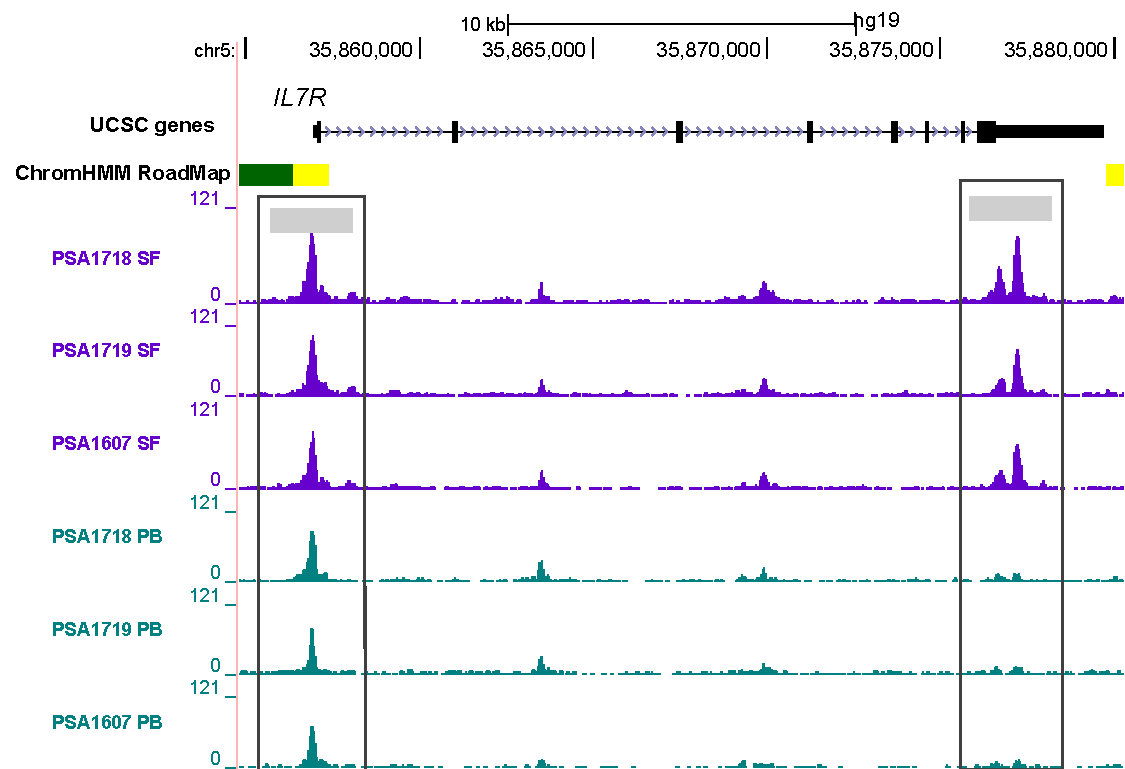
\includegraphics[width=\textwidth]{./Results3/pdfs/ATAC_PSA_CD14_IL7R}
\caption{}
\end{subfigure}
\caption[Differentially accessible regions located within gene bodies in CD14$^+$ monocytes and NK cells from PsA patients.]{\textbf{Differentially accessible regions located within gene bodies in CD14$^+$ monocytes and NK cells from PsA patients.} UCSC Genome Browser view illustrating the normalised ATAC read density (y-axis) in (A) DAR located at an intron of \textit{VAV3} gene (x-axis) in NK (less accessible in synovial fluid compared to peripheral blood) and (B) two DARs mapping to the 5' and 3'UTR of the \textit{IL7R}, respectively, in CD14$^+$ monocytes (both more accessible in synovial fluid compared to peripheral blood). Tracks are colour-coded by tissue (SF=purple; PB=turquoise). The Roadmap Epigenomics Project chromatin segmentation track for the appropriate cell type are also shown. All DARs were significant based on FDR$<$0.01 and FC$>$1.5.SF=synovial fluid; PB=peripheral blood.}
\label{figure:PsA_FAST_ATAC_gene_boy_DOCS_CD14_NK}
\end{figure}




\subsection{Pathway enrichment analysis highlights tissue functional differences in chromatin accessibility}

To explore the potential function of synovial fluid (synovial fluid open DARs) and peripheral blood (peripheral blood open DARs) specific accessibility changes in each cell type, gene annotation of each set of DARs was performed based on location (by physical proximity) as detailed in Chapter \ref{ch:Mat}, followed by pathway analysis. Despite common pathways enriched in both, a number of functionally relevant pathways appeared  significantly enriched (FDR$<$0.01 or 0.05) only for synovial fluid open DARs and not for peripheral blood open DARs and vice versa (Figure \ref{figure:PSA_ATAC_pathway_analysis_all_DOC}).
%Pathway enrichment analysis was conducted separately for synovial fluid open DARs and peripheral blood open DARs in each cell type. Gene annotation of the DARs was performed by physical proximity, as detailed in Chapter \ref{ch:Mat}. Despite commonalities, differences in significant enriched pathways (FDR$<$0.01 or 0.05) were also identified within the same cell type between synovial fluid and peripheral blood open DARs (Figure \ref{figure:PSA_ATAC_pathway_analysis_all_DOC}). 
In CD14$^+$ monocytes, synovial fluid open DARs showed enrichment for pathways involved in hemostasis, integrin interactions, calcium signalling and regulation of immunity, inflammation and cell survival, importantly the NF-$\kappa$B pathway (Figure \ref{figure:PSA_ATAC_pathway_analysis_all_DOC}A in purple). Synovial fluid open DARs in CD14$^+$ monocytes were also enriched for cytokine related pathways, including IL-2 and IL-3, IL-5 and granulocyte-macrophage colony stimulating factor (GM-CSF) signalling. By contrast, peripheral blood open DARs in CD14$^+$ monocytes were not enriched for any of these pathways, showing enrichment for DAP12 interactions and regulation of the PI3K/AKT network (Figure \ref{figure:PSA_ATAC_pathway_analysis_all_DOC}A in turquoise).

mCD4$^+$ synovial fluid open DARs, in contrast to peripheral blood, showed enrichment for TCR signalling as well as chemokine signalling,including DARs in proximity to IFN-$\gamma$ or \textit{CXCL13} and \textit{CXCR6}, respectively (Figure \ref{figure:PSA_ATAC_pathway_analysis_all_DOC}B in purple). Peripheral blood open DARs in this cell type were enriched for signalling by receptor tyrosine kinases and focal adhesion members, also involved in the T cell activation \parencite{Dustin2001}. Enriched pathways for synovial fluid or peripheral blood open DARs in mCD8$^+$ were only significant when using an FDR$<$0.05 threshold. The G protein coupled receptor (GPCR) signalling, with varied roles in regulation of inflammation and mediation of the chemotactic recruitment of T cells to the inflamed tissue, was enriched for mCD8$^+$ peripheral blood open DARs, as well as the Wnt signaling pathway %involved in the production of memory cells with enhanced proliferative potential and stronger protective capacity \parencite{Boudousquie2014}. 
(Figure \ref{figure:PSA_ATAC_pathway_analysis_all_DOC}C in turquoise). mCD8$^+$ synovial fluid open DARs showed enrichment for chemokine signalling and regulation of stem cell pluripotency (Figure \ref{figure:PSA_ATAC_pathway_analysis_all_DOC}C in purple).  



\begin{figure}[H]
\centering
\begin{subfigure}[b]{0.48\textwidth}
\centering 
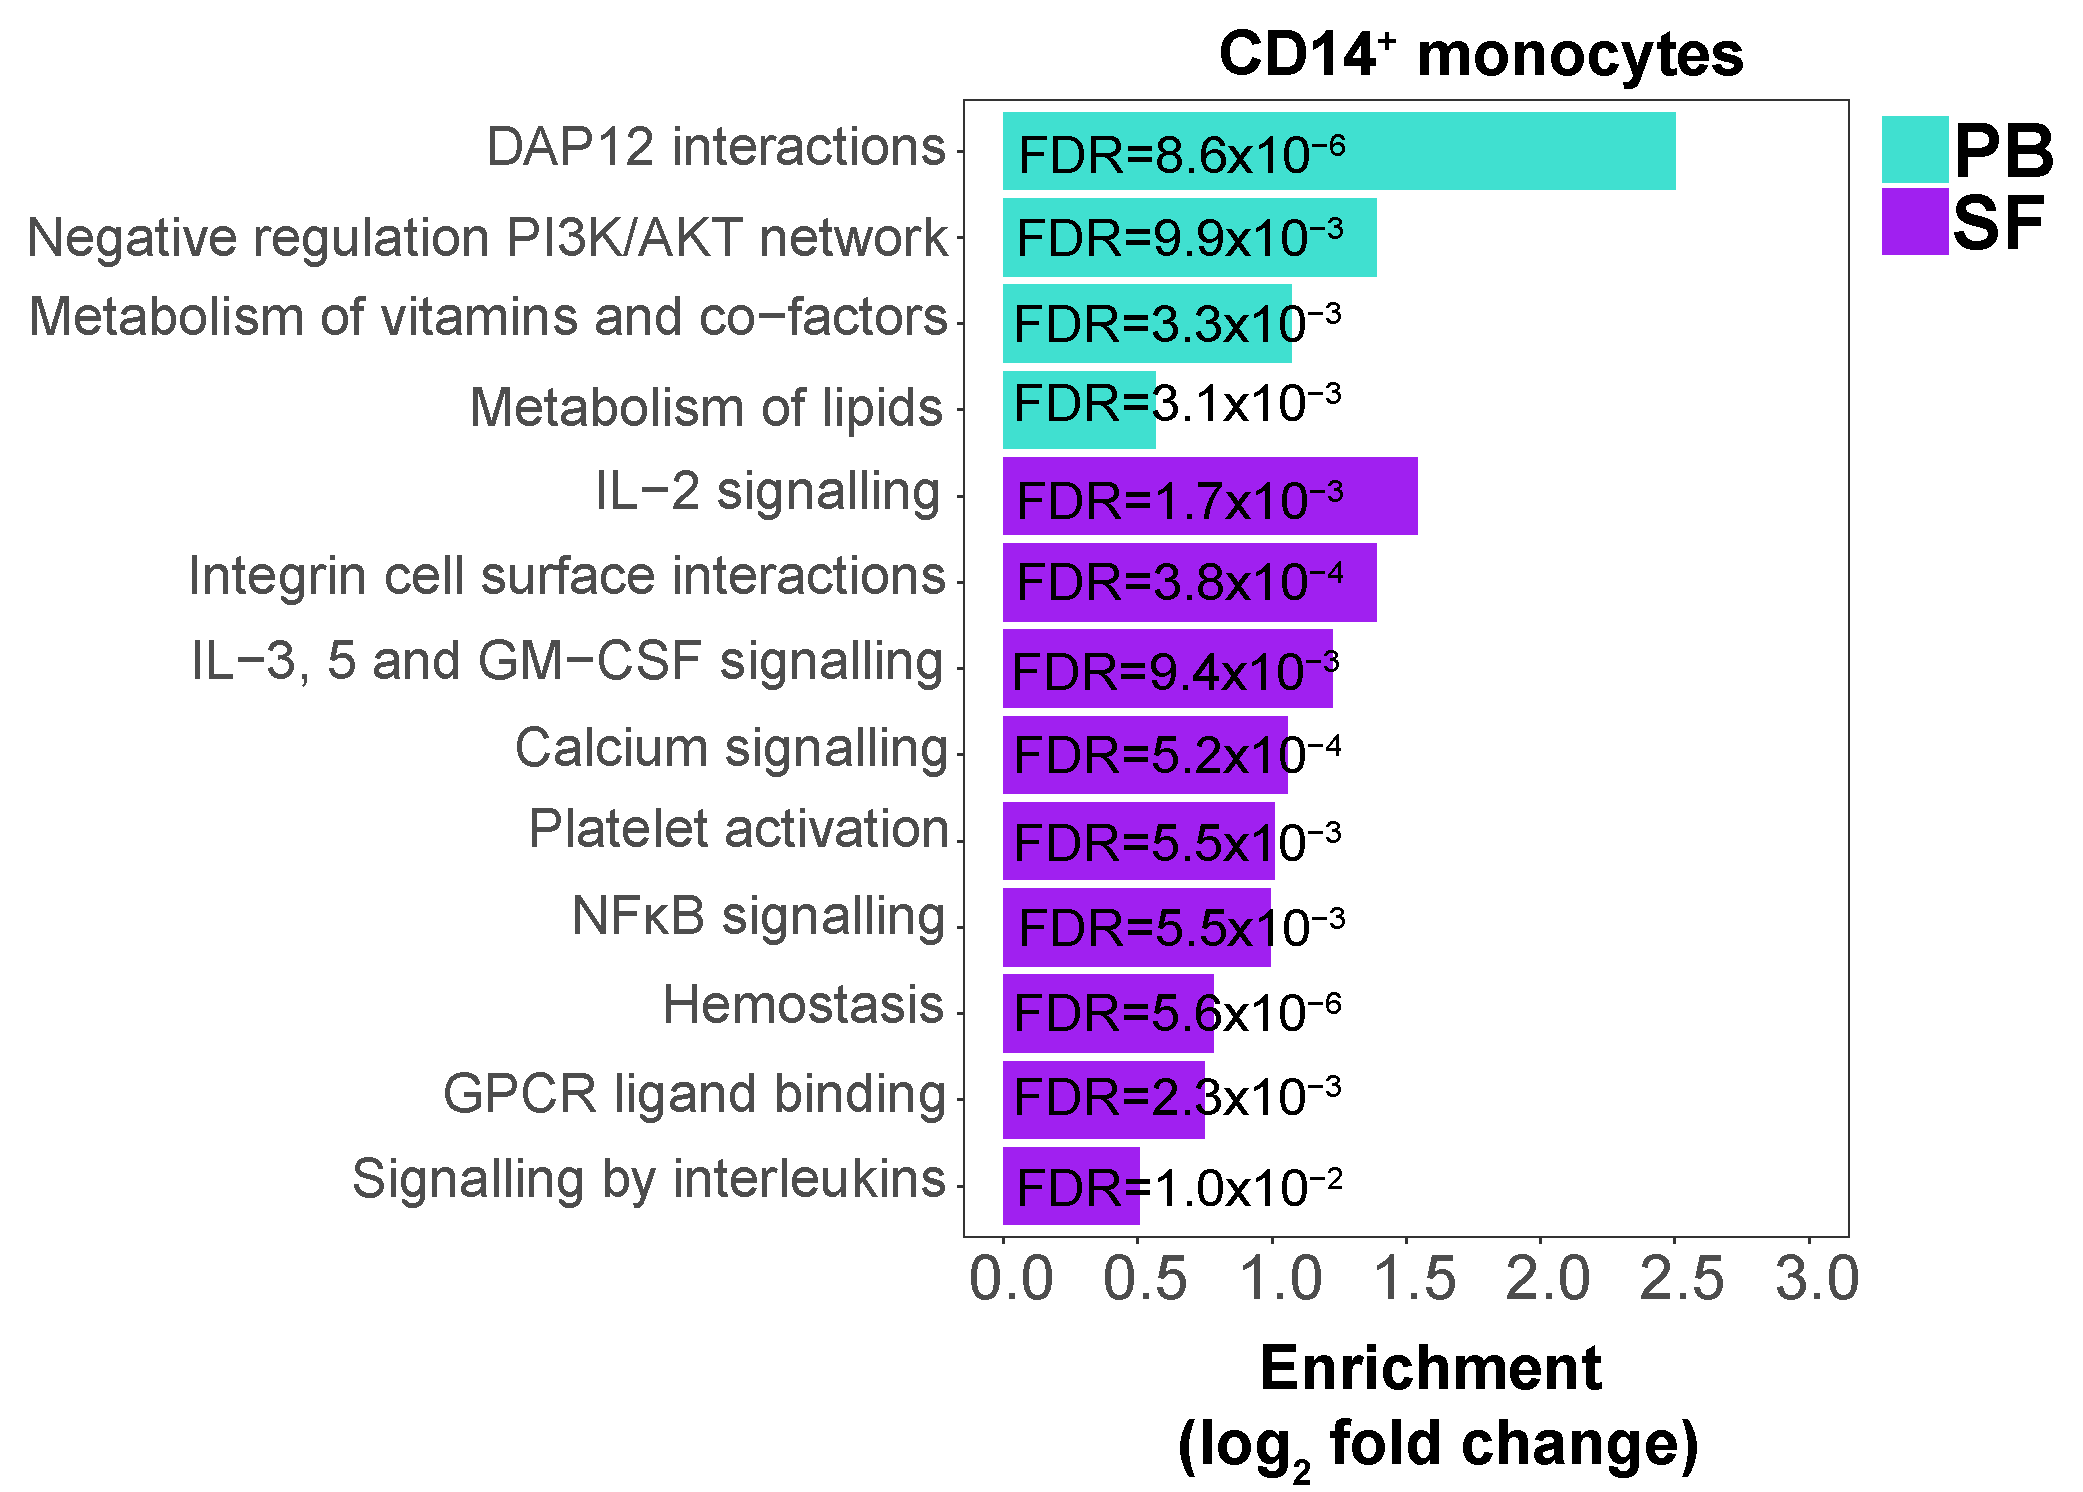
\includegraphics[width=\textwidth]{./Results3/pdfs/ATAC_PSA_CD14_pathways_barplot_all_DOCS_proximity_FC}
\caption{}
\end{subfigure}
~
\begin{subfigure}[b]{0.48\textwidth}
\centering 
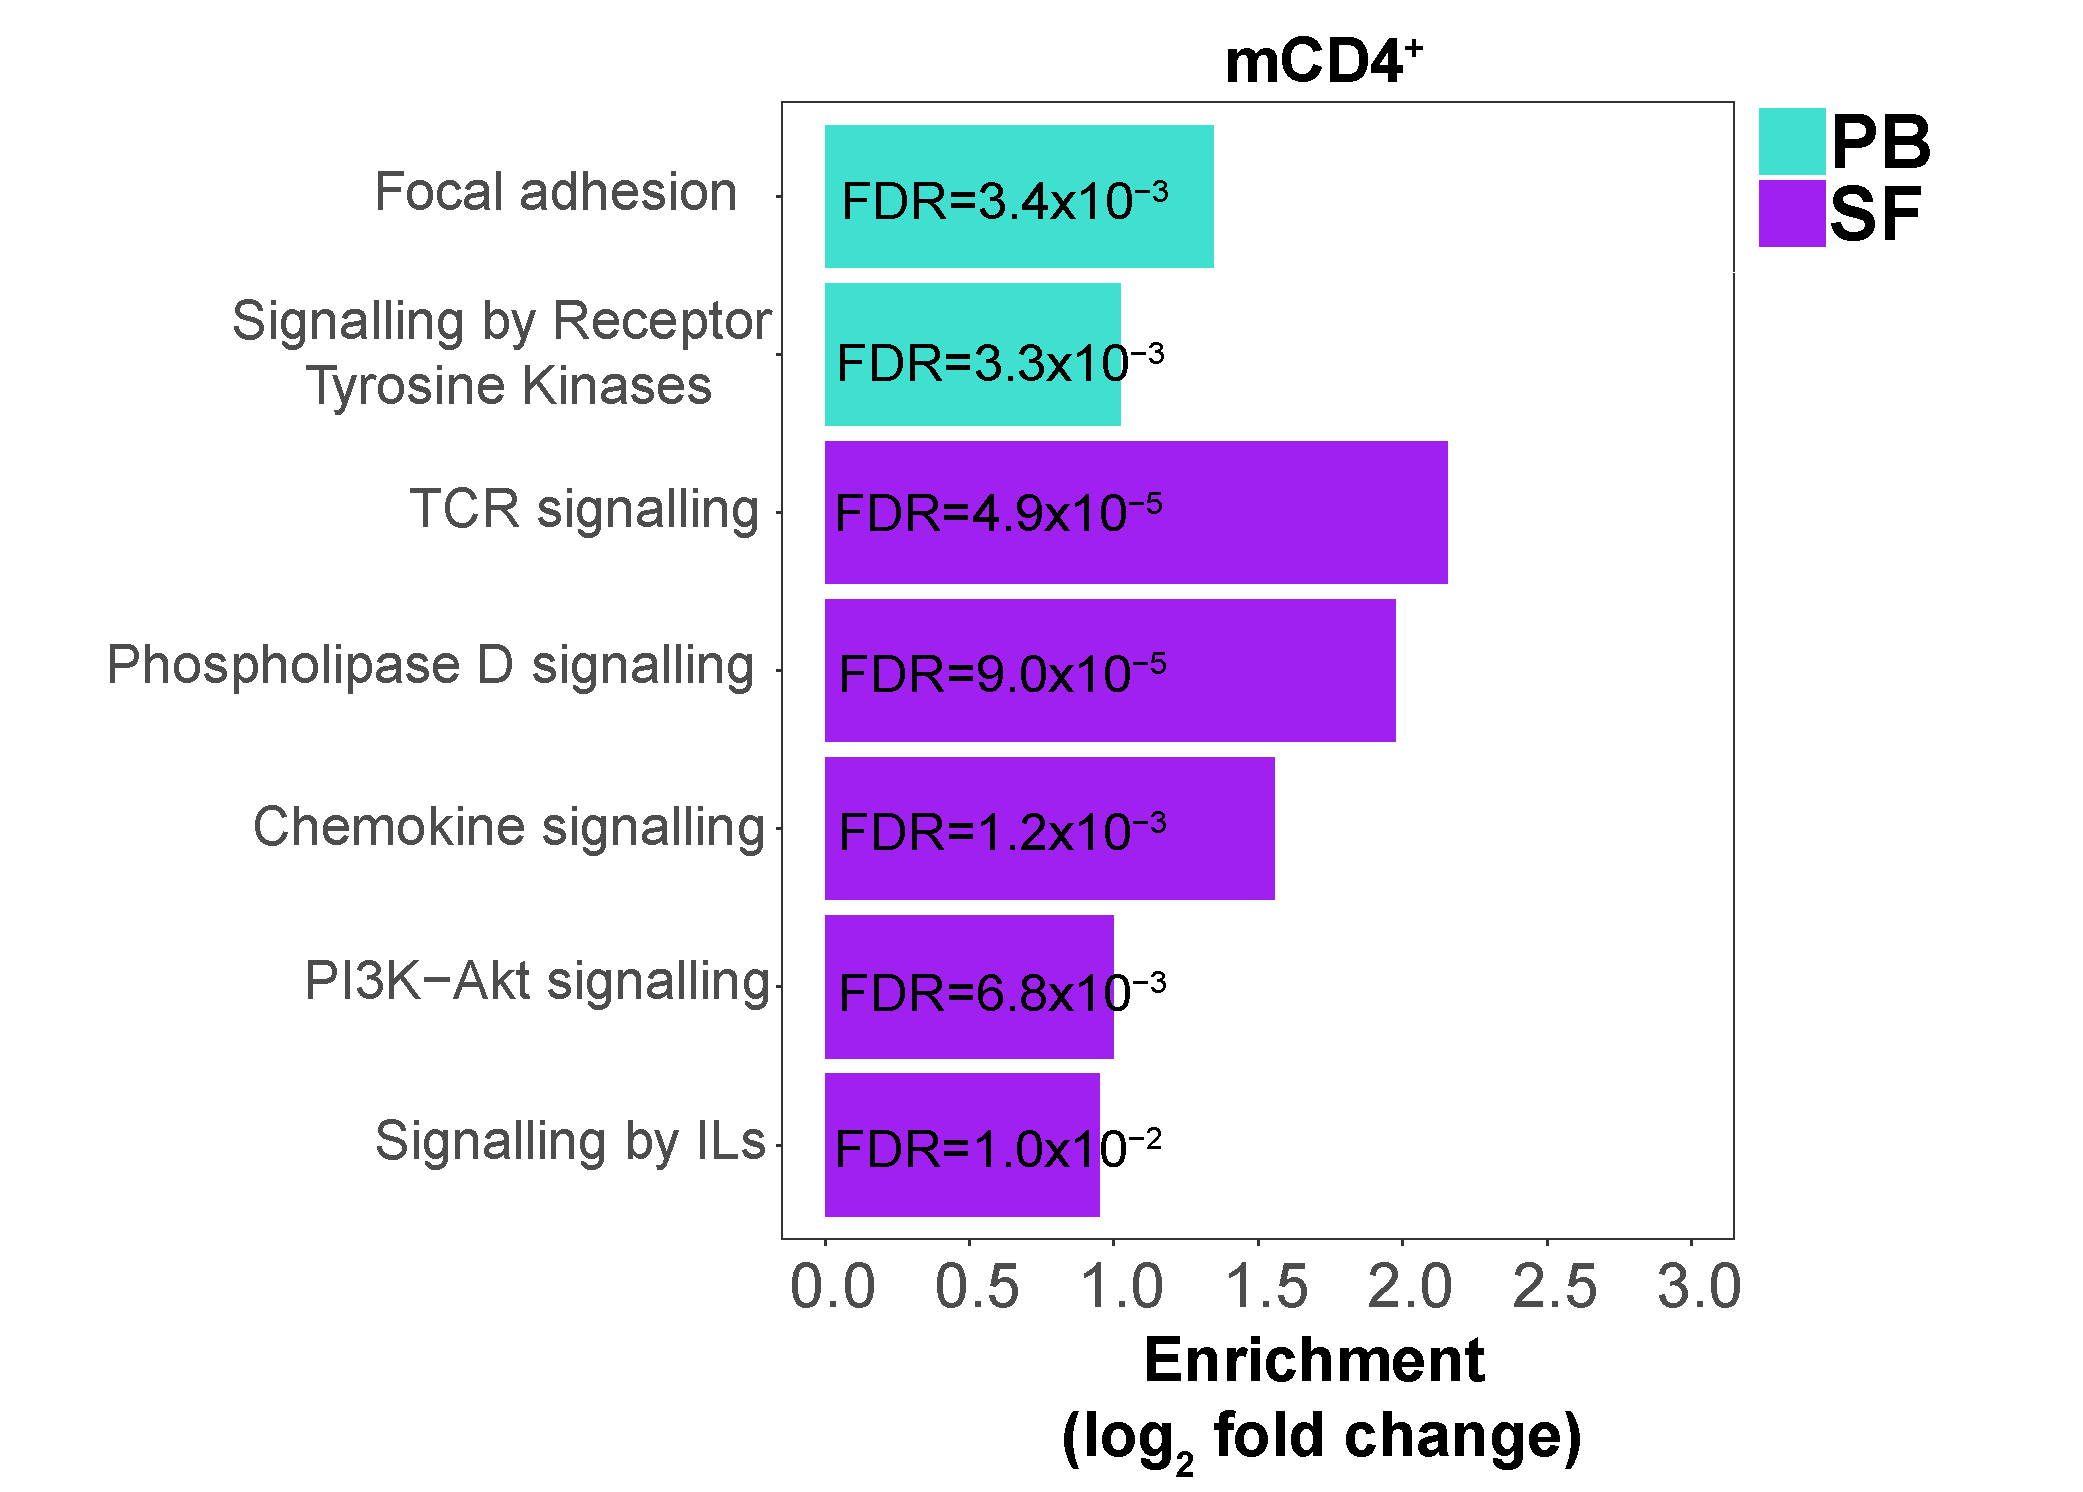
\includegraphics[width=\textwidth]{./Results3/pdfs/ATAC_PSA_CD4_pathways_barplot_all_DOCS_proximity_FC}
\caption{}
\end{subfigure}
~
\begin{subfigure}[b]{0.48\textwidth} 
%the [b] prevents offset in subcaptions
\centering
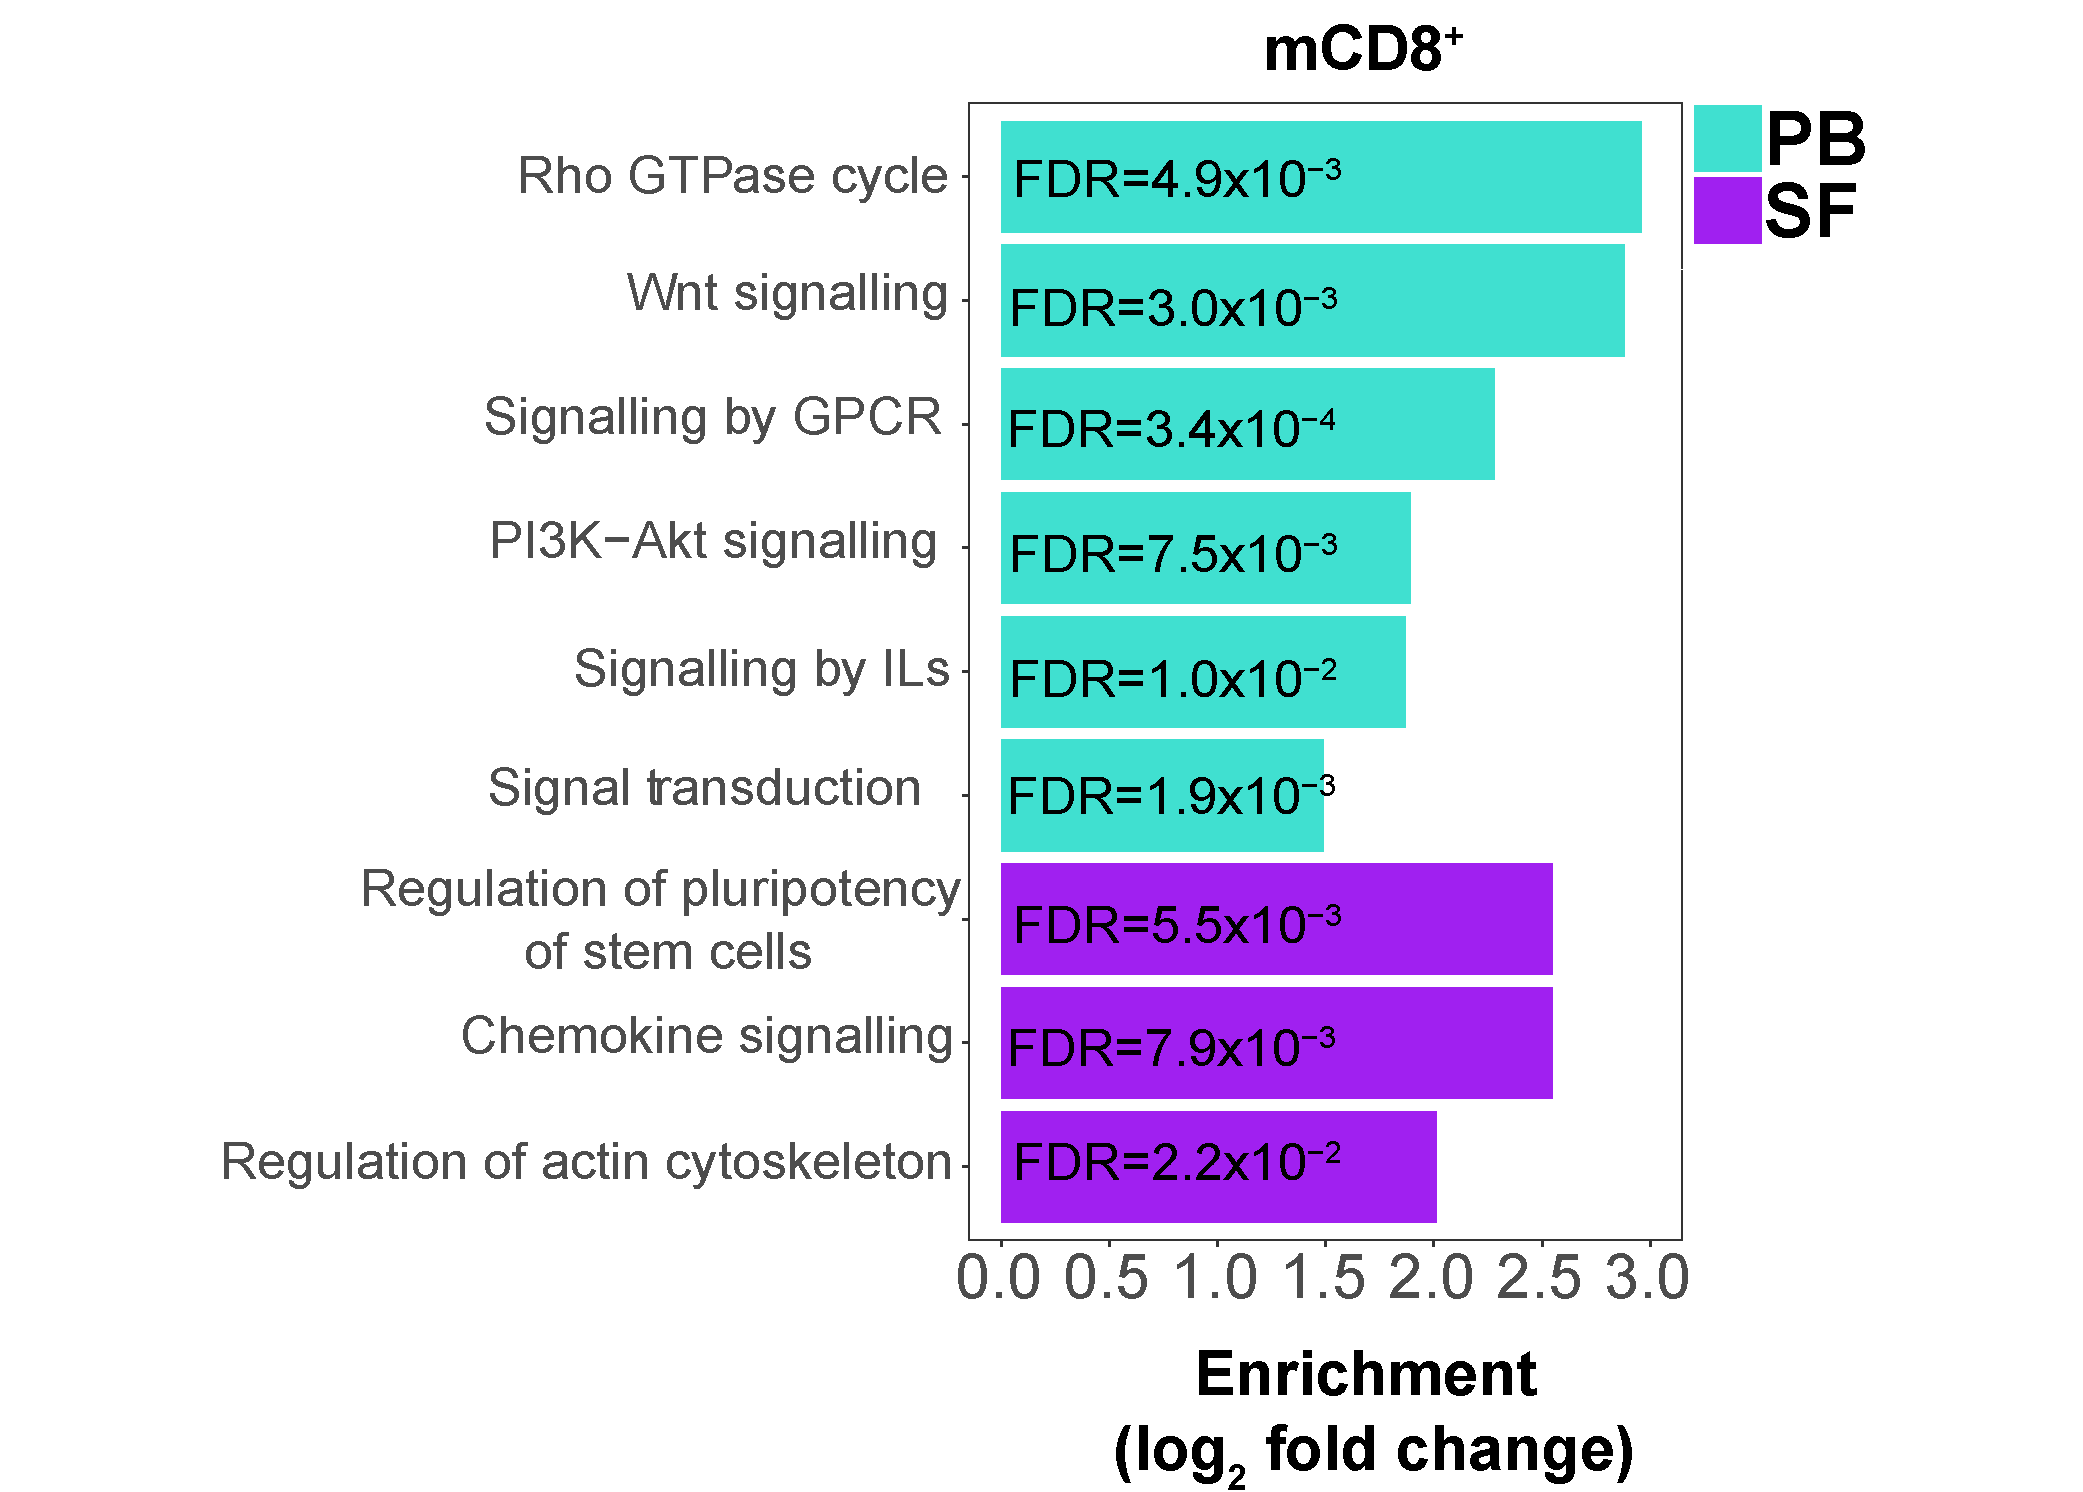
\includegraphics[width=\textwidth]{./Results3/pdfs/ATAC_PSA_CD8_pathways_barplot_all_DOCS_proximity_FC}%
\caption{}
\end{subfigure}
\begin{subfigure}[b]{0.48\textwidth} 
%the [b] prevents offset in subcaptions
\centering
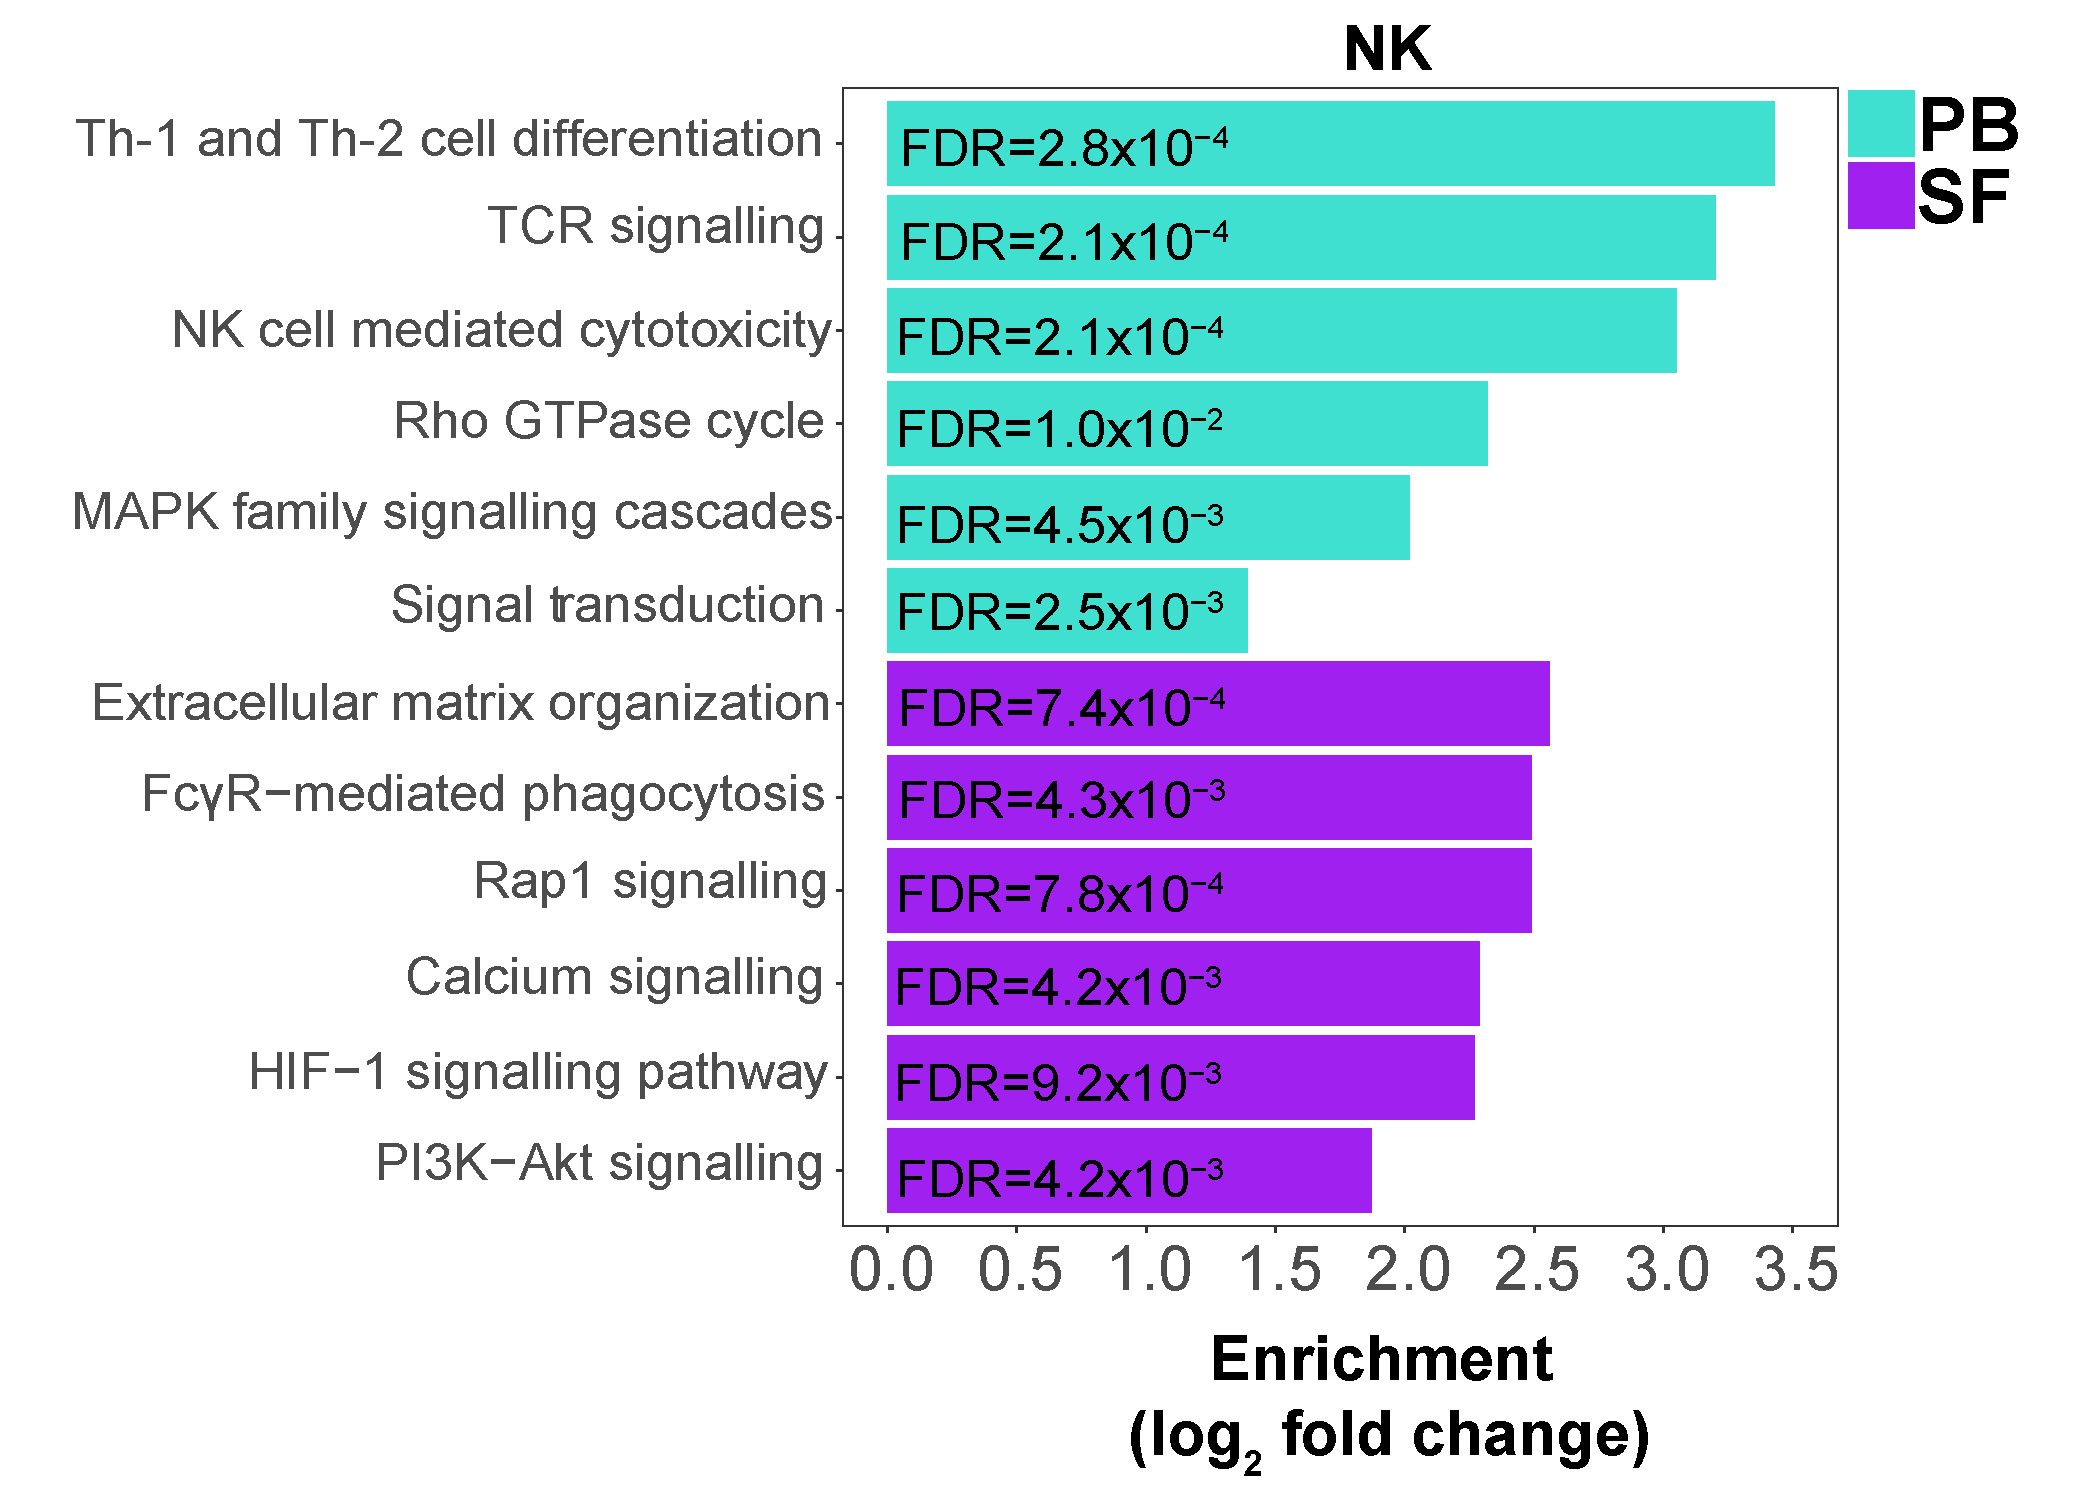
\includegraphics[width=\textwidth]{./Results3/pdfs/ATAC_PSA_NK_pathways_barplot_all_DOCS_proximity_FC}%
\caption{}
\end{subfigure}
\caption[Functional pathways significantly enriched and unique for either synovial fluid open or peripheral blood open DARs in CD14$^+$ monocytes, CD4m$^+$,CD8m$^+$ and NK cells.]{\textbf{Functional pathways significantly enriched and unique for either synovial fluid open or peripheral blood open DARs in CD14$^+$ monocytes, CD4m$^+$,CD8m$^+$ and NK cells.} Enrichment analysis was performed separately for genes annotating synovial fluid open DARs and peripheral blood open DARs. Log$_2$ fold change of unique functionally relevant significant pathways (FDR $<$0.01 or 0.05) enriched for synovial fluid open DARs or peripheral blood open DARs in (A) CD14$^+$ monocytes, (B) mCD4$^+$, (C) mCD8$^+$ and (D) NK cells are shown. SF=synovial fluid; PB=peripheral blood.}
\label{figure:PSA_ATAC_pathway_analysis_all_DOC}
\end{figure}

NK synovial fluid open DARs showed enrichment for extracellular matrix organisation and RAP-1 signalling as well as for Fc$\gamma$ receptor (FC$\gamma$R)-mediated phagocytosis (Figure \ref{figure:PSA_ATAC_pathway_analysis_all_DOC}D in purple). Members of the HIF-1 pathway involved in oxygen homeostasis were also enriched in NK synovial fluid open DARs, in line with the hypoxic environment found in joint inflammation. Interestingly, enrichment of open peripheral blood DARs in the proximity of genes involved in NK-mediated toxicity was found (Figure \ref{figure:PSA_ATAC_pathway_analysis_all_DOC}D in turquoise). 
% NK CD56 bright subsets and tissue http://www.jimmunol.org/content/196/7/2923.long
% Production of IgG in PsA http://www.jrheum.org/content/41/12/2421.long
% NK phagocytisis FCgamma R III https://www.ncbi.nlm.nih.gov/pmc/articles/PMC1550276/, https://www.sciencedirect.com/science/article/pii/S0022202X15300373#bb0030, https://www.sciencedirect.com/science/article/pii/S0022202X15300373#bb0185
%Joint hypoxia https://www.ncbi.nlm.nih.gov/pmc/articles/PMC3683428/
%Skin hypoxia https://www.sciencedirect.com/science/article/pii/S0022202X15331328?via%3Dihub




%\begin{figure}[htbp]
%\centering
%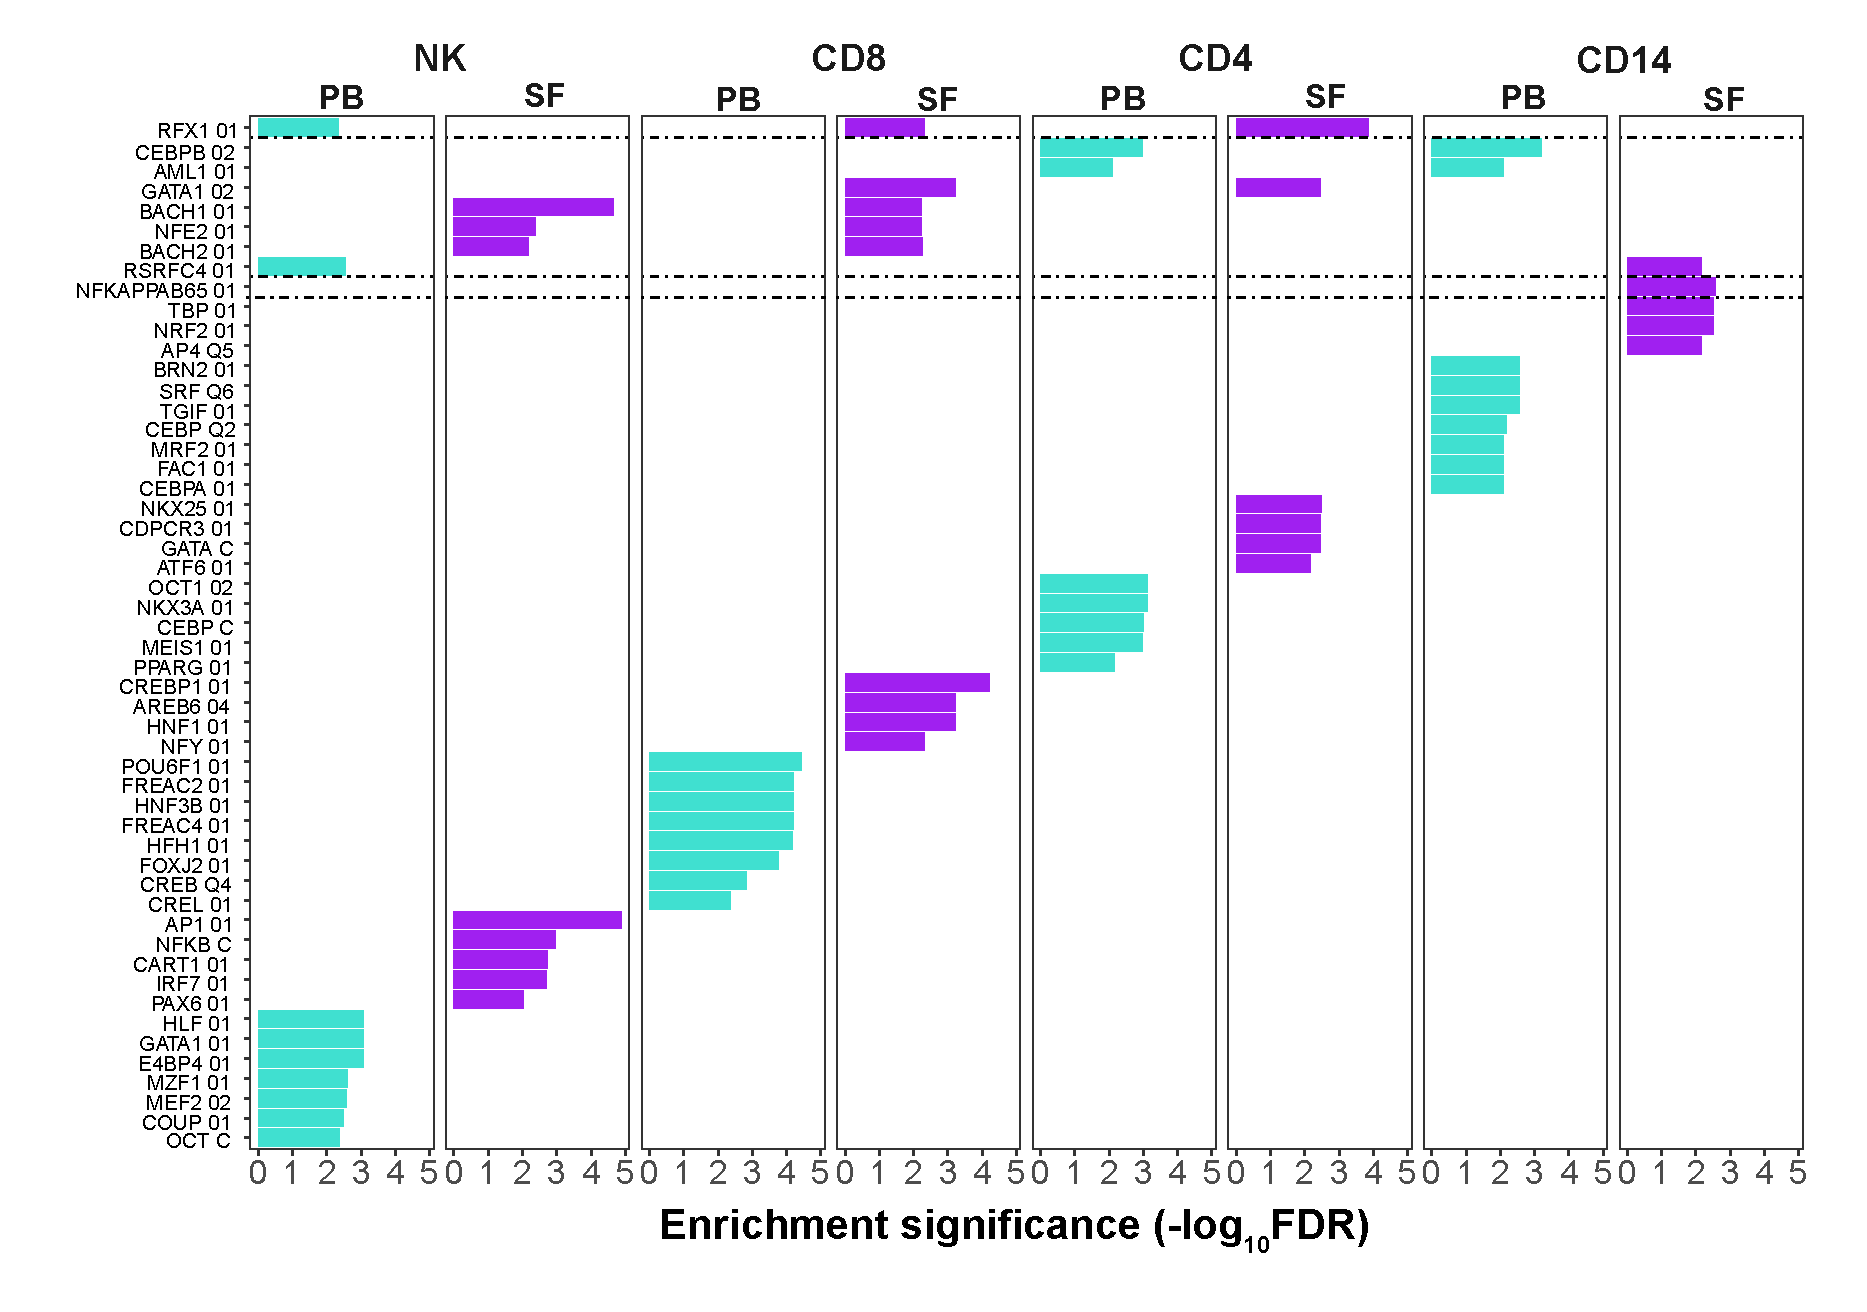
\includegraphics[width=0.8\textwidth]{./Results3/pdfs/ATAC_PSA_enrichment_conserved_TFBS_barplots_cell_type_specific_DOCS_all_cell_types_per_tissue}
%\caption[Enrichment of eRNA cell type-specific PsA DARs for conserved TFBS.]{\textbf{Enrichment of eRNA cell type-specific PsA DARs for conserved TFBS.} xxxx }
%\label{figure:PSA_TFBS}
%\end{figure}



\subsection{Differential gene expression analysis in paired circulating and synovial immune cells}

\subsubsection{Immune-relevant gene expression by qPCR}
%Introductory paragraph to link to ATAC-seq data
%Mapping chromatin accessibility represents an informative tool to identify regulatory elements undergoing histone modifications, DNA methylation and TF binding, as previously explained. All those elements are involved in the regulation of gene expression, making the study of chromatin accessibility a good proxy for the inference of gene expression. Nevertheless, the characterisation of the chromatin landscape also presents some limitations, including the discordance between open chromatin and functionality of the regulatory element, shown by CAGE studies, as well as the identification of the target gene regulated by a particular element. 

In order to contextualise the ATAC data, qPCR gene expression analysis for 370 key genes in the inflammatory and autoimmune response was conducted in CD14$^+$ monocytes, mCD4$^+$ and mCD8$^+$ cells isolated from synovial fluid and peripheral blood of three PsA patients (Table \ref{tab:PSA_datasets_per_sample}). %Those appeared as the most abundant cell types in peripheral blood and synovial fluid from patients, and particularly mCD4$^+$ and mCD8$^+$ cells have been shown to expand in PsA inflammed synovium, as previously mentioned. 


\begin{figure}[htbp]
\centering
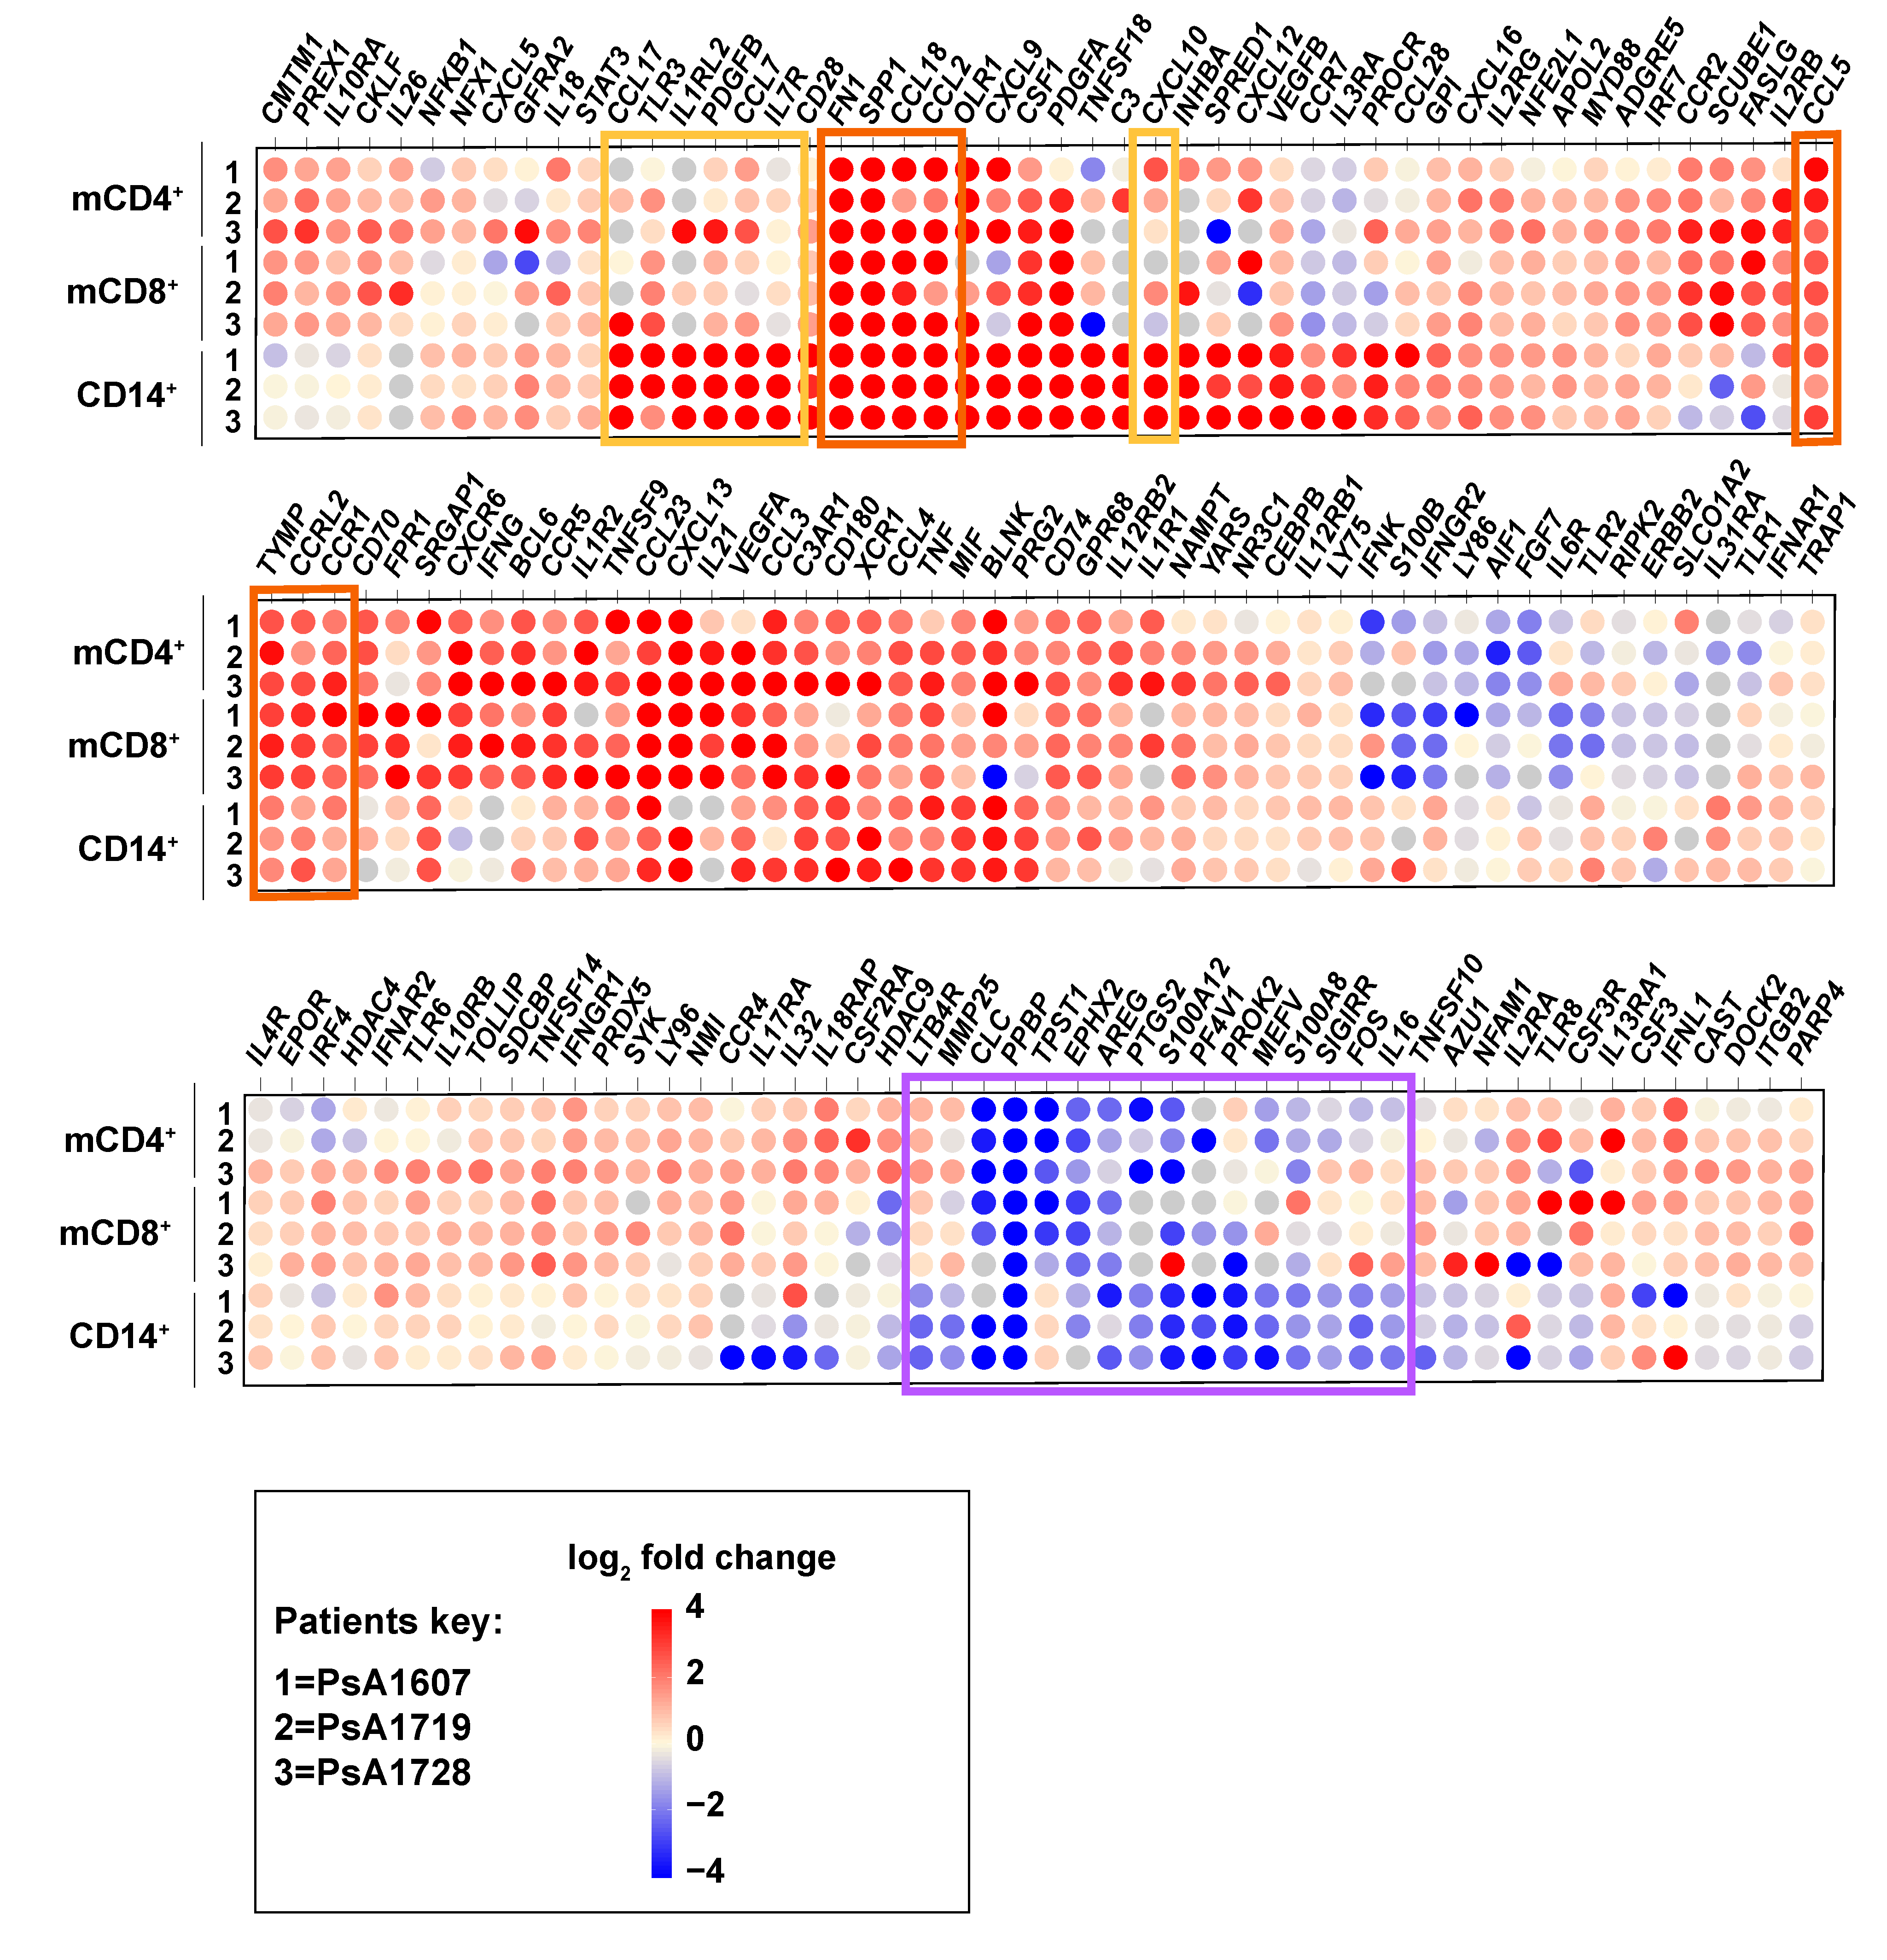
\includegraphics[width=\textwidth]{./Results3/pdfs/PCR_array_PSA_SF_vs_PB_filtered_5_percent_genes_heatmap_final}
\caption[Heatmap illustrating fold changes in gene expression between synovial fluid and peripheral blood across CD14$^+$ monocytes and mCD4$^+$ and mCD8$^+$ T cells.]{\textbf{Heatmap illustrating fold changes in gene expression between synovial fluid and peripheral blood across CD14$^+$ monocytes and mCD4$^+$ and mCD8$^+$ T cells.} Amongst the 370 genes measured by qPCR, the fold change in gene expression between the synovial fluid and peripheral blood for each pair of samples is represented only for those genes which were consistently modulated across the 3 PsA samples (p-value$<$0.05) in at least one of the cell types. Each column represents a genes and each row a pair of synovial fluid-peripheral blood PsA samples. The log$_{2}$ fold change in gene expression between synovial fluid and peripheral blood is colour-coded. For visualisation purposes the heatmap is shown in 3 distinct blocks. PsA identity is included.}
\label{figure:PSA_PCR_array_5_pcnt_heatmap}
\end{figure}

%\begin{landscape}
%\begin{figure}[H]
%\centering
%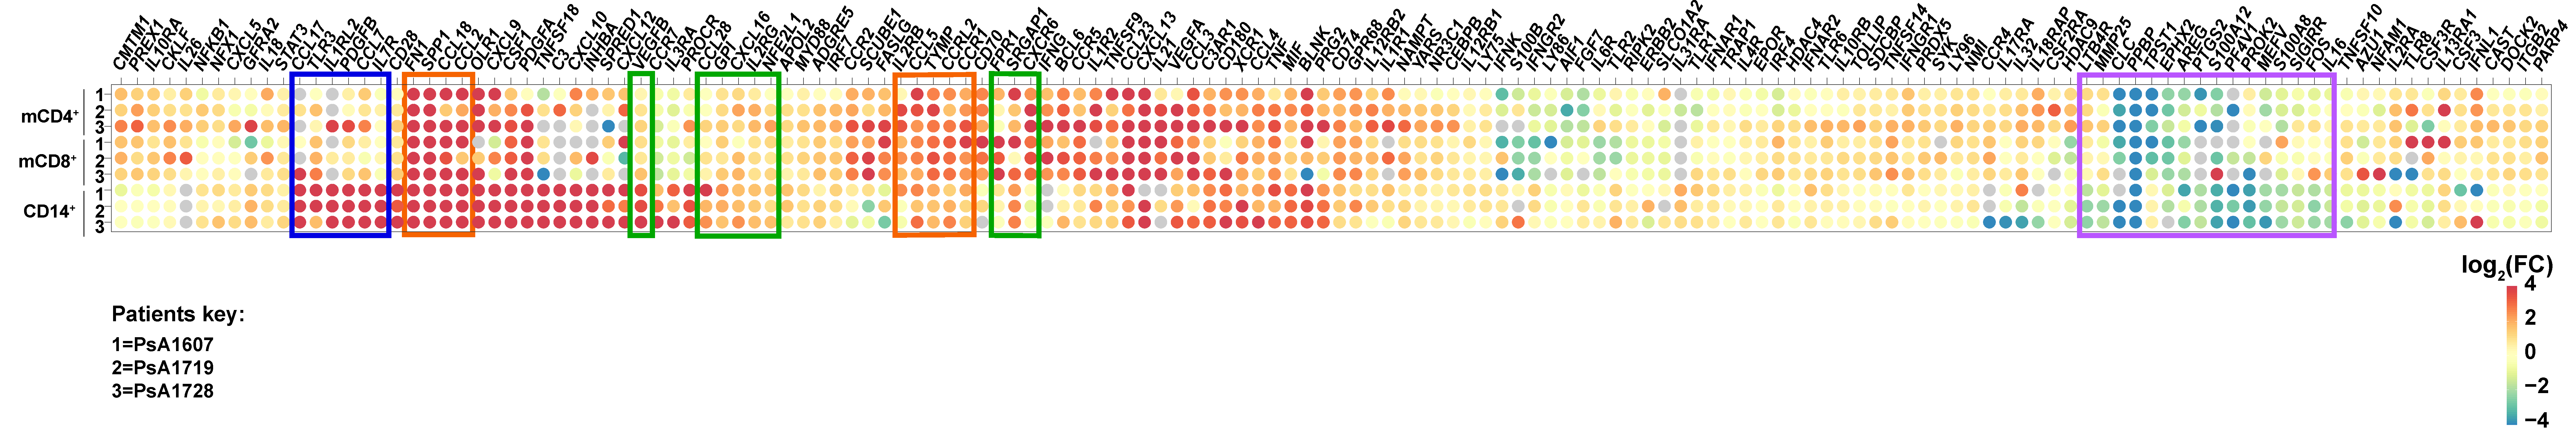
\includegraphics[width=1.5\textwidth]{./Results3/pdfs/PCR_array_PSA_SF_vs_PB_filtered_5_percent_genes_heatmap_New}
%\caption[Heatmap of gene expression FCs between synovial fluid and peripheral blood for those gene significantly modulated (p-value$<$0.05) in at least one cell type.]{\textbf{Heatmap of gene expression fold changes between synovial fluid and peripheral blood for those gene significantly modulated (p-value$<$0.05) in at least one cell type.} Amongst the 370 genes measured by qPCR, the fold change in gene expression between the synovial fluid and peripheral blood for each pair of samples has been represented only those genes which were consistently modulated across the three PsA samples (p-value$<$0.05) in at least one of the cell types. Each column represents a genes and each row a pair of synovial fluid-peripheral blood PsA samples. The log$_{2}fold change$ in gene expression between synovial fluid and peripheral blood is colour-coded. Overall, the heatmap allows to observe the change in gene expression as well as the magnitude between synovial fluid and peripheral blood for each gene in each of the the three pairs of PsA samples in CD14$^+$ monocytes, mCD4$^+$ and mCD8$^+$ cells.}
%\label{figure:PSA_PCR_array_5_pcnt_heatmap}
%\end{figure}
%\end{landscape}

The PCR array represented a cost-effective approach to study gene expression between peripheral blood and synovial fluid focusing on a relevant subset of genes, given the inflammatory component in PsA. For each cell types, fold change in expression was calculated pair-wise for synovial fluid respect to peripheral blood within each sample for each individual genes (detailed in Chapter \ref{ch:Mat}).  Fold change in gene expression showed differences in magnitude and reproducibility between the three cell types (Figure \ref{figure:PSA_PCR_array_5_pcnt_heatmap}). Genes showing marked up-regulation (fold change$>$1.5) in the three cell types when comparing synovial fluid vs peripheral blood were found, for example \textit{FN1}, \textit{SPP1} or \textit{CCL2}, amongst others (Figure \ref{figure:PSA_PCR_array_5_pcnt_heatmap} orange box). On the other hand, genes presenting reduced expression in synovial fluid (fold change$<$1.5) in at least one of the three cell types were observed, including \textit{FOS}, \textit{IL16}, \textit{PPBP} and \textit{TPST1} (Figure \ref{figure:PSA_PCR_array_5_pcnt_heatmap} purple box). Genes demonstrating consistent changes in the same direction in the three CD14$^+$ monocyte samples but not in T cells were also identified (Figure \ref{figure:PSA_PCR_array_5_pcnt_heatmap} dark yellow box). These included up-regulation of \textit{CXCL10} and \textit{IL7R} in the synovial fluid of CD14$^+$ monocytes compared to peripheral blood that were inconsistent in mCD4$^+$ and mCD8$^+$ T cells. Moreover, differences in fold change were also observed for genes modulated in the same direction across the three cell types, for instance \textit{VEGFB} and \textit{CCL17} (Figure \ref{figure:PSA_PCR_array_5_pcnt_heatmap}).

Changes in expression did not reach significance after multiple testing correction (FDR$<$0.05 or 0.1) for the majority of the genes assayed by the qPCR array, likely due to the small sample size. Following this, filtering using a p-value$<$0.05 as the statistical threshold for significance and a mean fold change$>$1.5, CD14$^+$ monocytes and mCD8$^+$ showed greater number of significantly modulated genes (72 and 77, respectively) compared to mCD4$^+$ cells (46 genes) (Figure \ref{figure:PSA_PCR_array_vulcano_plots}A, B and C). In all three cell types, most of the dysregulated immune genes were up-regulated in the synovial fluid compared to peripheral blood (Figure \ref{figure:PSA_PCR_array_vulcano_plots}A, B and C). For example, 56 out of the 70 significantly modulated genes in CD14$^+$ monocytes showed mean fold change$>$1.5 vs the 14 genes with mean fold change$<$1.5 (Figure \ref{figure:PSA_PCR_array_vulcano_plots}A).

% May need a bit more of biology there
\begin{figure}[htbp]
\centering
\begin{subfigure}{0.48\textwidth}
\centering
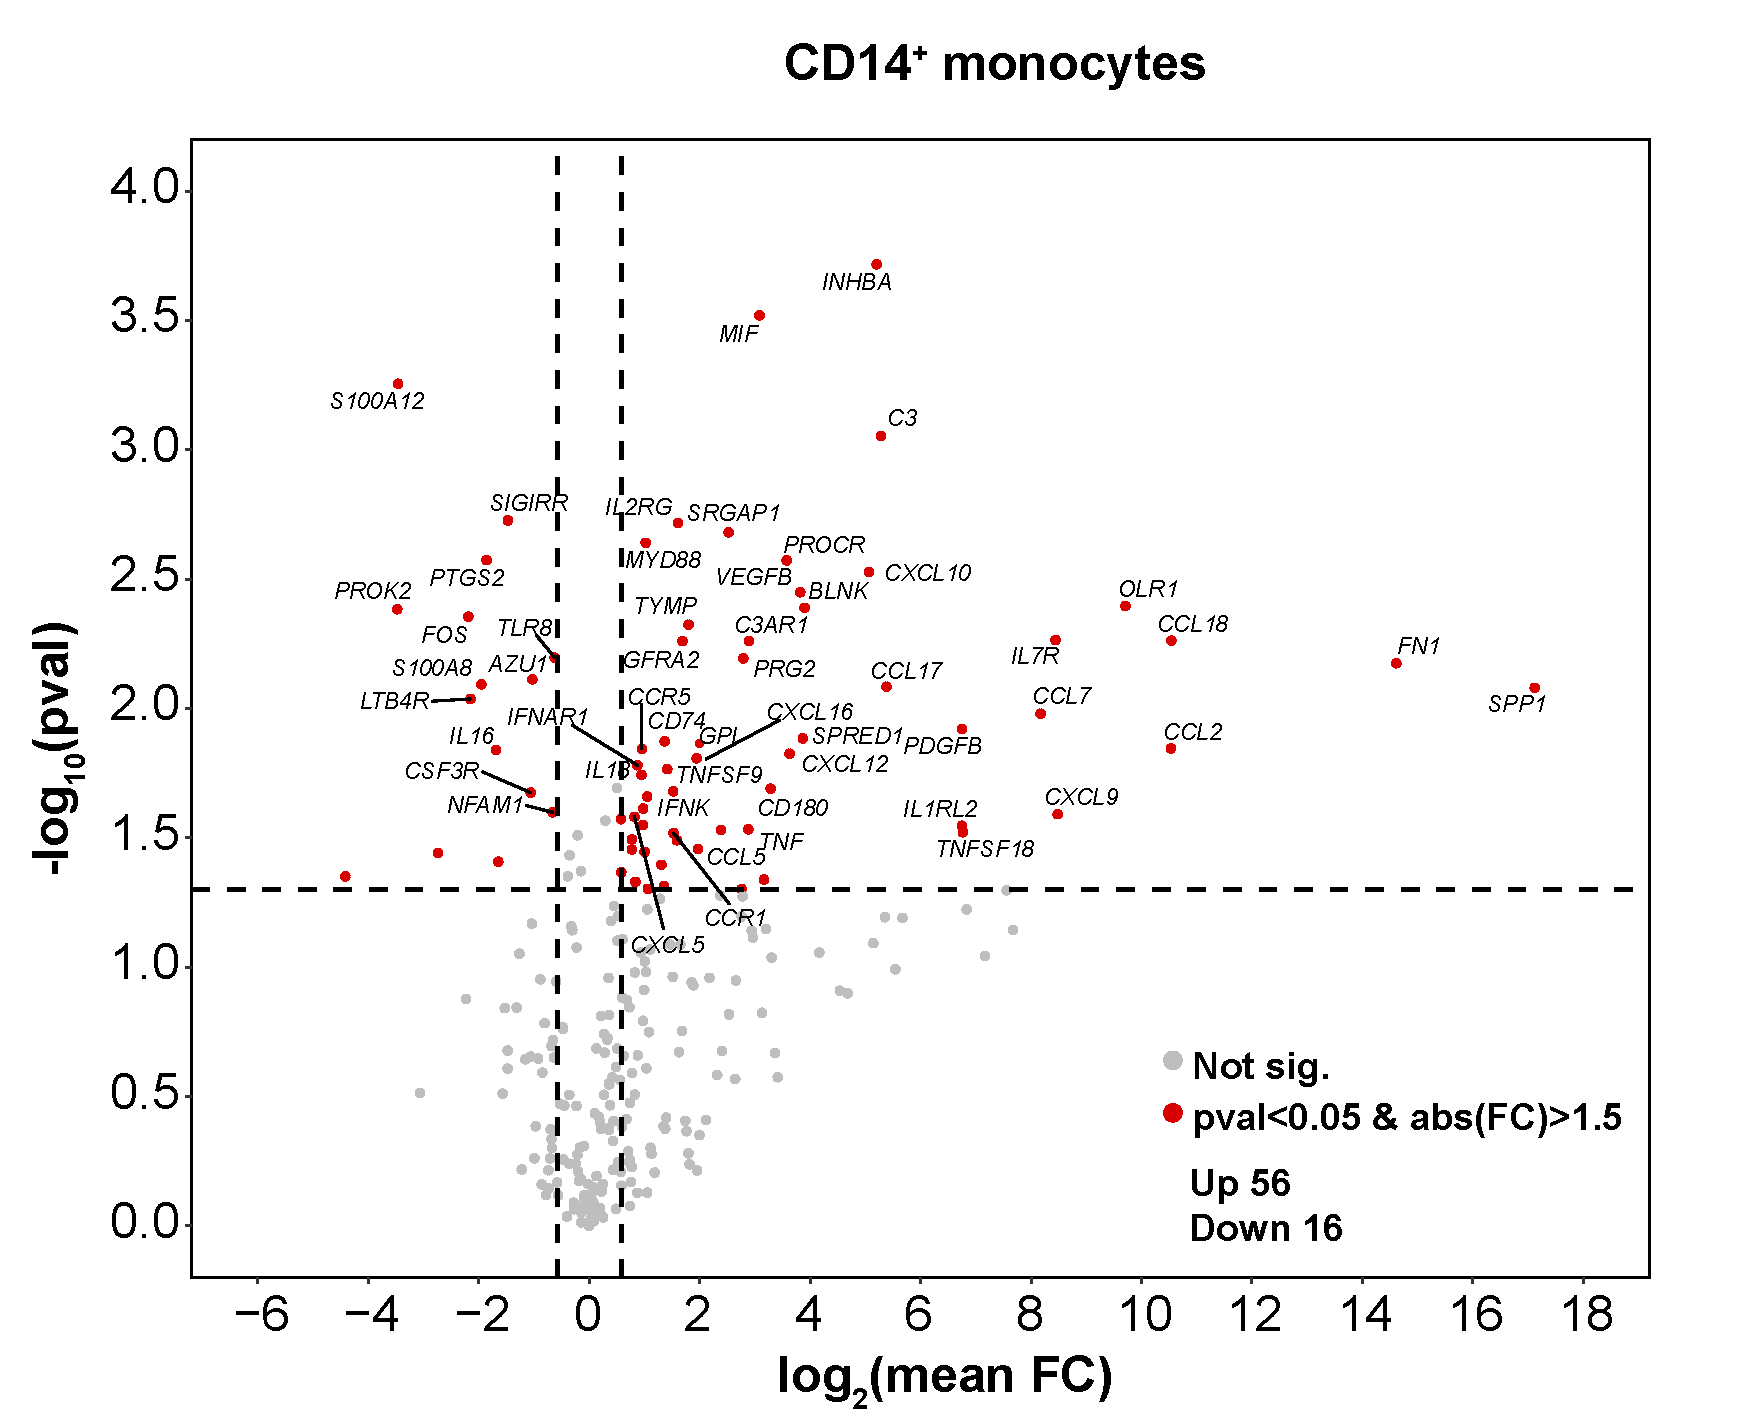
\includegraphics[width=\textwidth]{./Results3/pdfs/PSA_CD14_vulcano_plot_PCR_array_mean_FC}
\caption{\textbf{}}
% The percentage sign indicated that the other subfig goes side by side
\end{subfigure}%
\begin{subfigure}{0.48\textwidth}
\centering
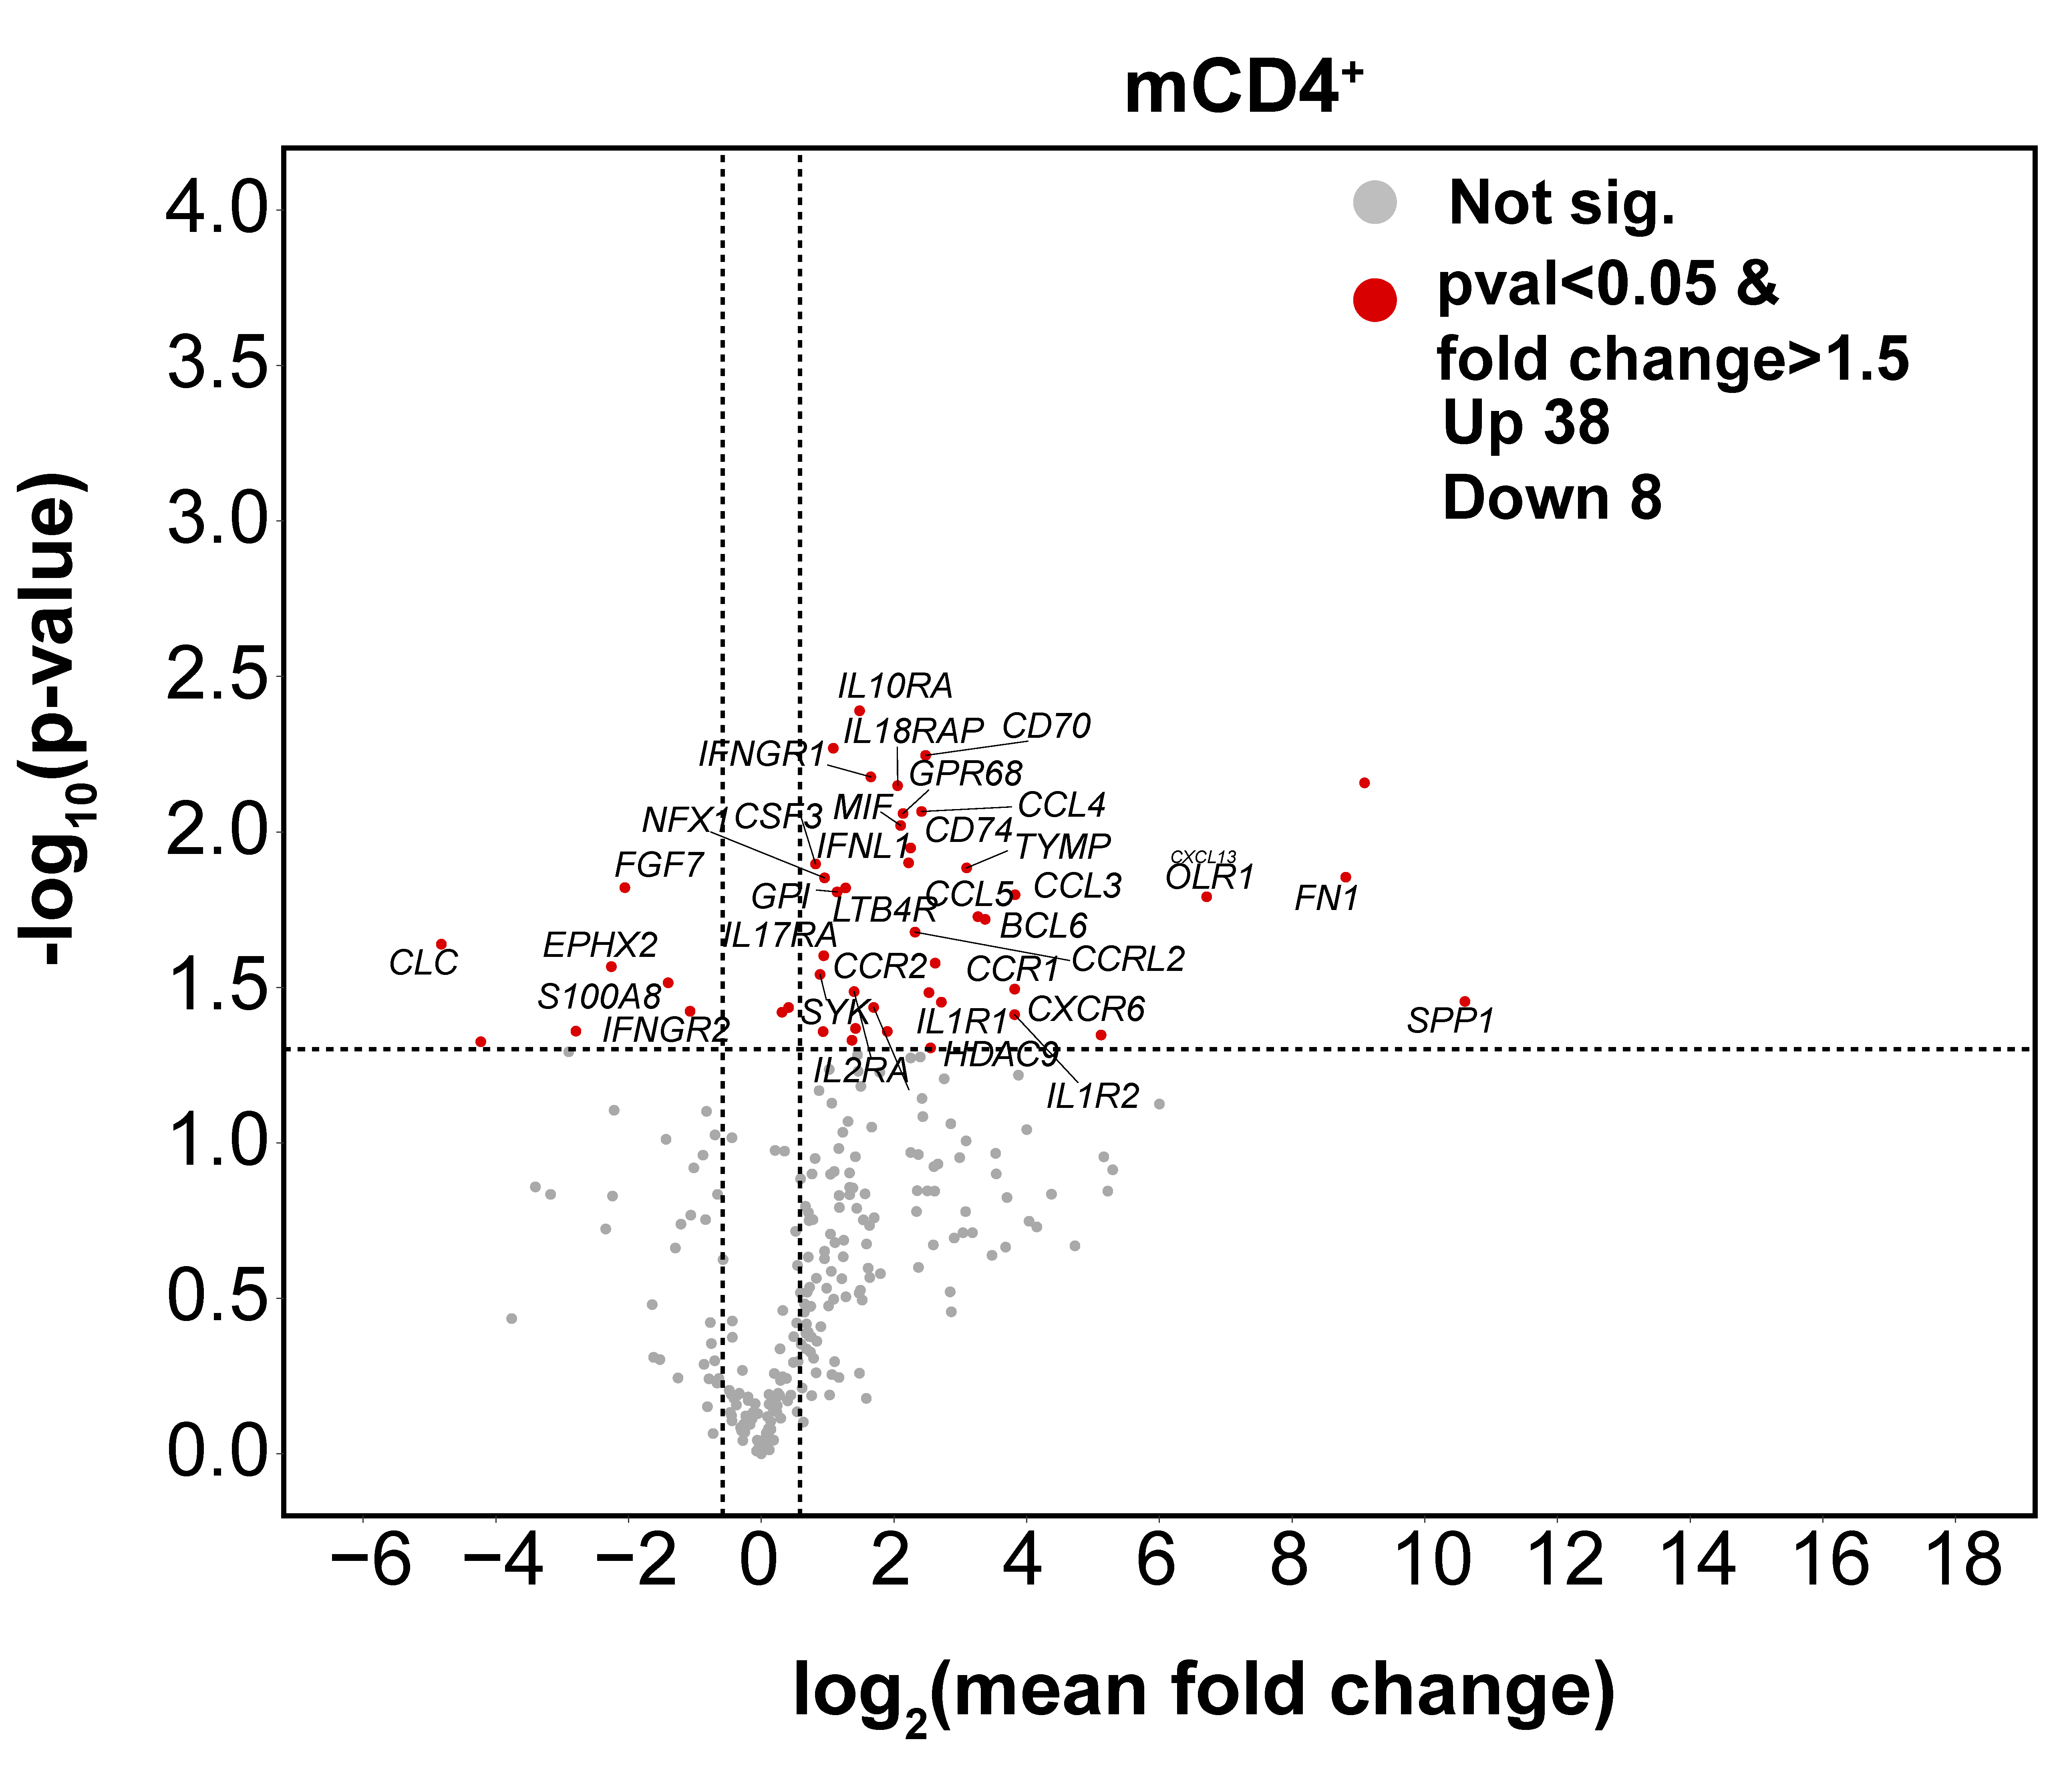
\includegraphics[width=\textwidth]{./Results3/pdfs/PSA_CD4_vulcano_plot_PCR_array_mean_FC}
\caption{\textbf{}}
\end{subfigure}
\begin{subfigure}{0.48\textwidth}
\centering
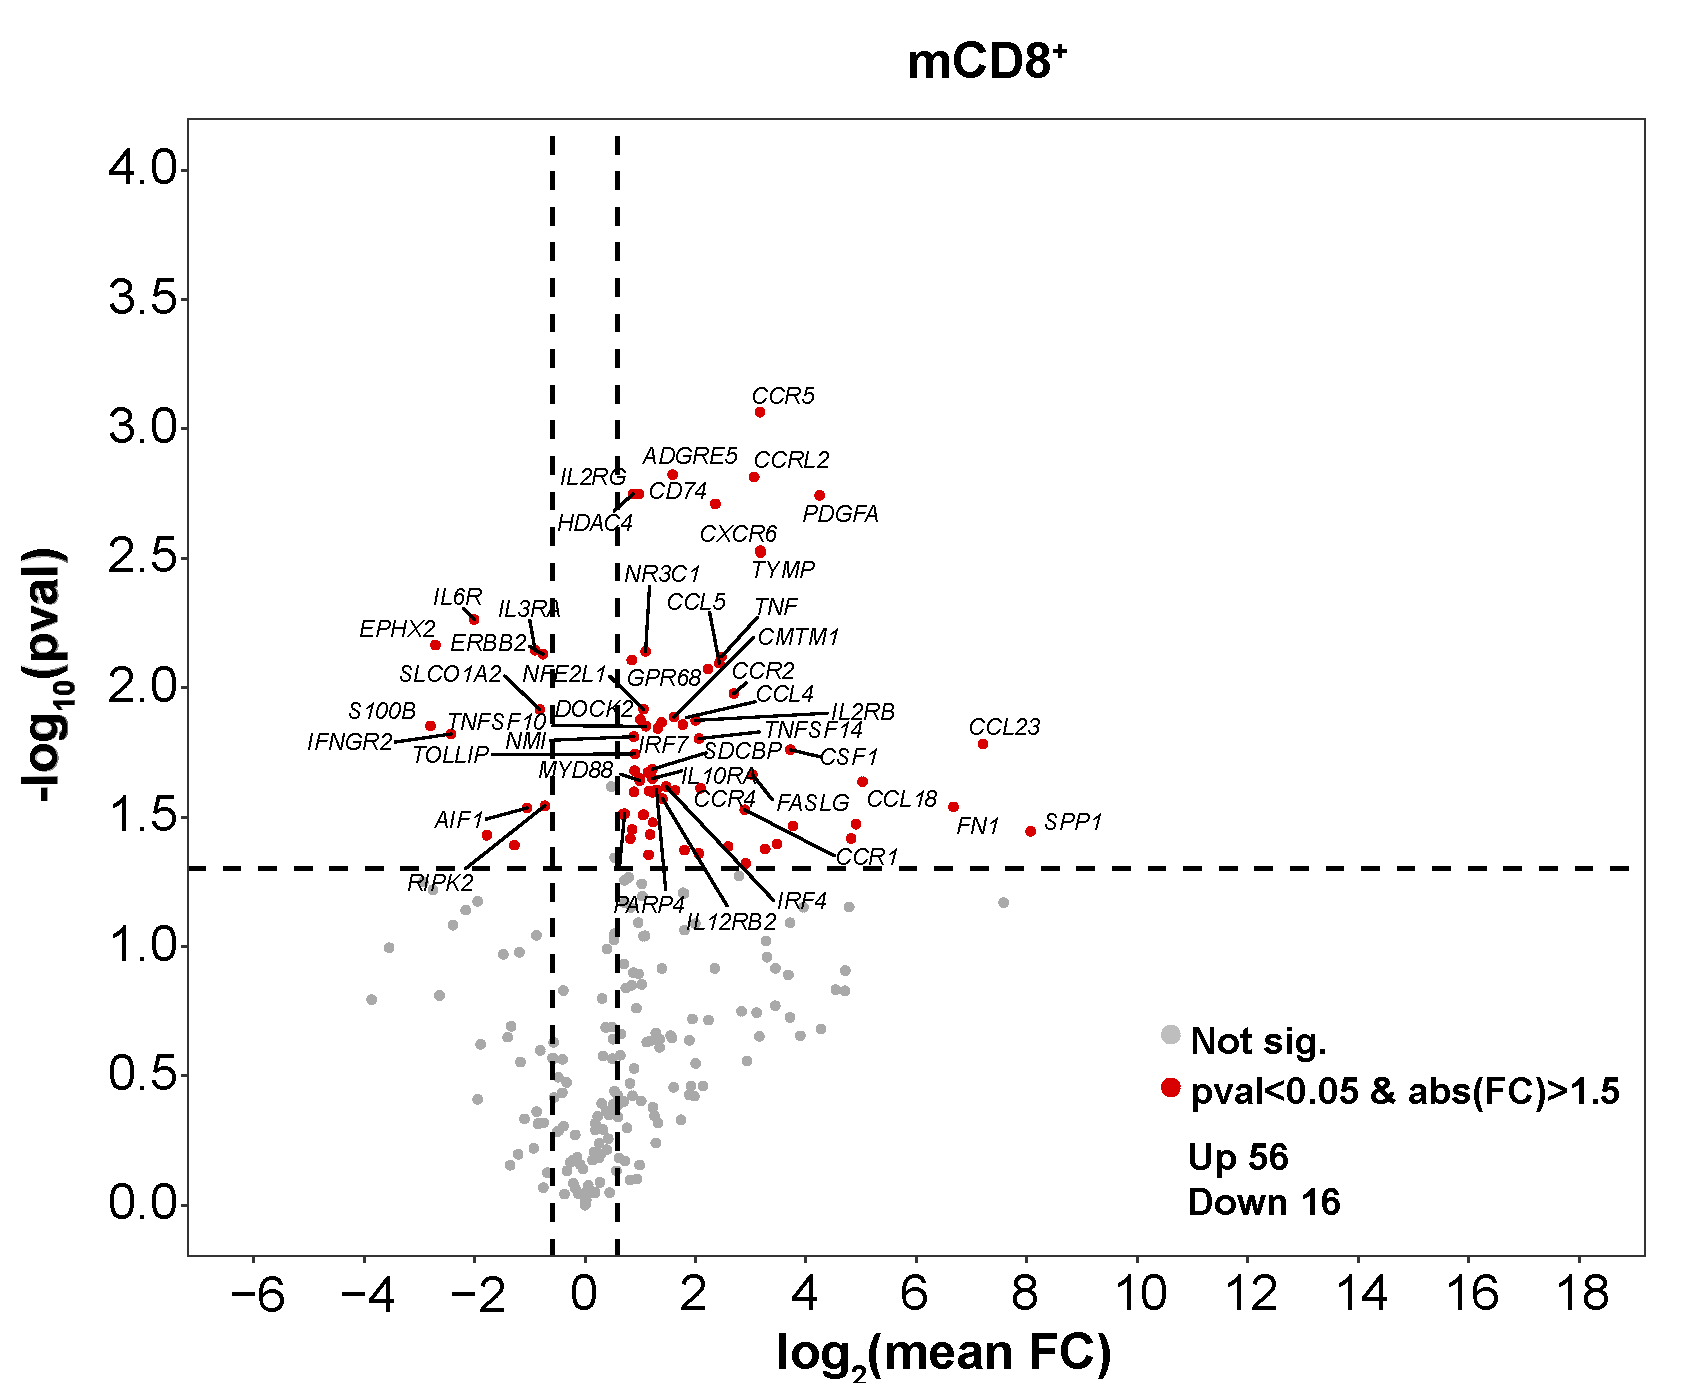
\includegraphics[width=\textwidth]{./Results3/pdfs/PSA_CD8_vulcano_plot_PCR_array_mean_FC}
\caption{\textbf{}}
\end{subfigure}
\caption[Gene expression changes in immune-relevant genes between synovial fluid and peripheral blood in CD14$^+$ monocytes, mCD4$^+$ and mCD8$^+$ cells.]{\textbf{Gene expression changes in immune-relevant genes between synovial fluid and peripheral blood in CD14$^+$ monocytes, mCD4$^+$ and mCD4$^+$ cells.} Volcano plots showing differences in gene expression measured by qPCR array between synovial fluid and peripheral blood for (A) CD14$^+$ monocytes, (B) mCD4$^+$ and (C) mCD8$^+$ cells. The significance (log$_{10}$p-value) of the modulation in gene expression between the two tissues (y-axis) is plotted against the log${_2}$ of the mean fold change across the three PsA patients. Positive fold change indicates higher expression in synovial fluid. Genes showing p-value$<$0.05 and mean fold change$>$1.5 in red, with the most significant genes labelled. orange=up-regulated in the three cell types; purple=down-regulated in at least one cell type; yellow=consistent changes in CD14$^+$ monocytes only.}
\label{figure:PSA_PCR_array_vulcano_plots}
\end{figure} 



Gene expression in peripheral blood of the three PsA patients was also compared to peripheral blood of the three healthy controls for CD14$^+$ monocytes, mCD4$^+$ and mCD8$^+$ cells. P-values and fold changes were calculated between the mean peripheral blood expression across the three PsA patients and the mean expression of the three healthy controls for each of the genes in the array (as detailed in Chapter \ref{ch:Mat}). Integration of the differentially expressed (and therefore modulated genes) between synovial fluid and peripheral blood in PsA and and those changing expression between peripheral blood of PsA and healthy controls allowed the identification of three group of genes (Figure \ref{figure:PSA_PCR_array_HC_FC_correlation}). 

Firstly, the genes solely modulated in peripheral blood between controls and PsA were designated as systemic genes (Figure \ref{figure:PSA_PCR_array_HC_FC_correlation} green dots). These genes were not significantly expressed between synovial fluid and peripheral blood in PsA patients, and could then be considered as the circulating disease ``footprint''. For example \textit{CCL24} and \textit{CCL27} in CD14$^+$ monocytes. A second group of genes were designated as tissue-specific, since they were significantly modulated between synovial fluid and peripheral blood in PsA patients but did not show significant changes between controls and PsA at the circulating level (Figure \ref{figure:PSA_PCR_array_HC_FC_correlation} red dots). This group included \textit{CCR10} in mCD8$^+$ cells plus \textit{SPP1} and \textit{FN1} in the three cell types. These two genes demonstrated the largest fold changes in expression between synovial fluid and peripheral blood and presented no statistically significant differential expression in peripheral blood when comparing PsA and healthy controls. The third category comprised genes significantly modulated for each cell type between controls and PsA patients in peripheral blood, as well as between synovial fluid and peripheral blood in PsA patients. These genes were defined as putative disease-specific genes (Figure \ref{figure:PSA_PCR_array_HC_FC_correlation} blue dots), for example \textit{GPR68} in mCD4$^+$ cells (Figure \ref{figure:PSA_PCR_array_HC_FC_correlation} B). Nevertheless, this analysis is clearly limited by the lack of comparison to synovial fluid from a non-related disease as well as by the small sample size and the quantification of a limited number of genes.


\begin{figure}[htbp]
\centering
\begin{subfigure}{0.45\textwidth}
\centering
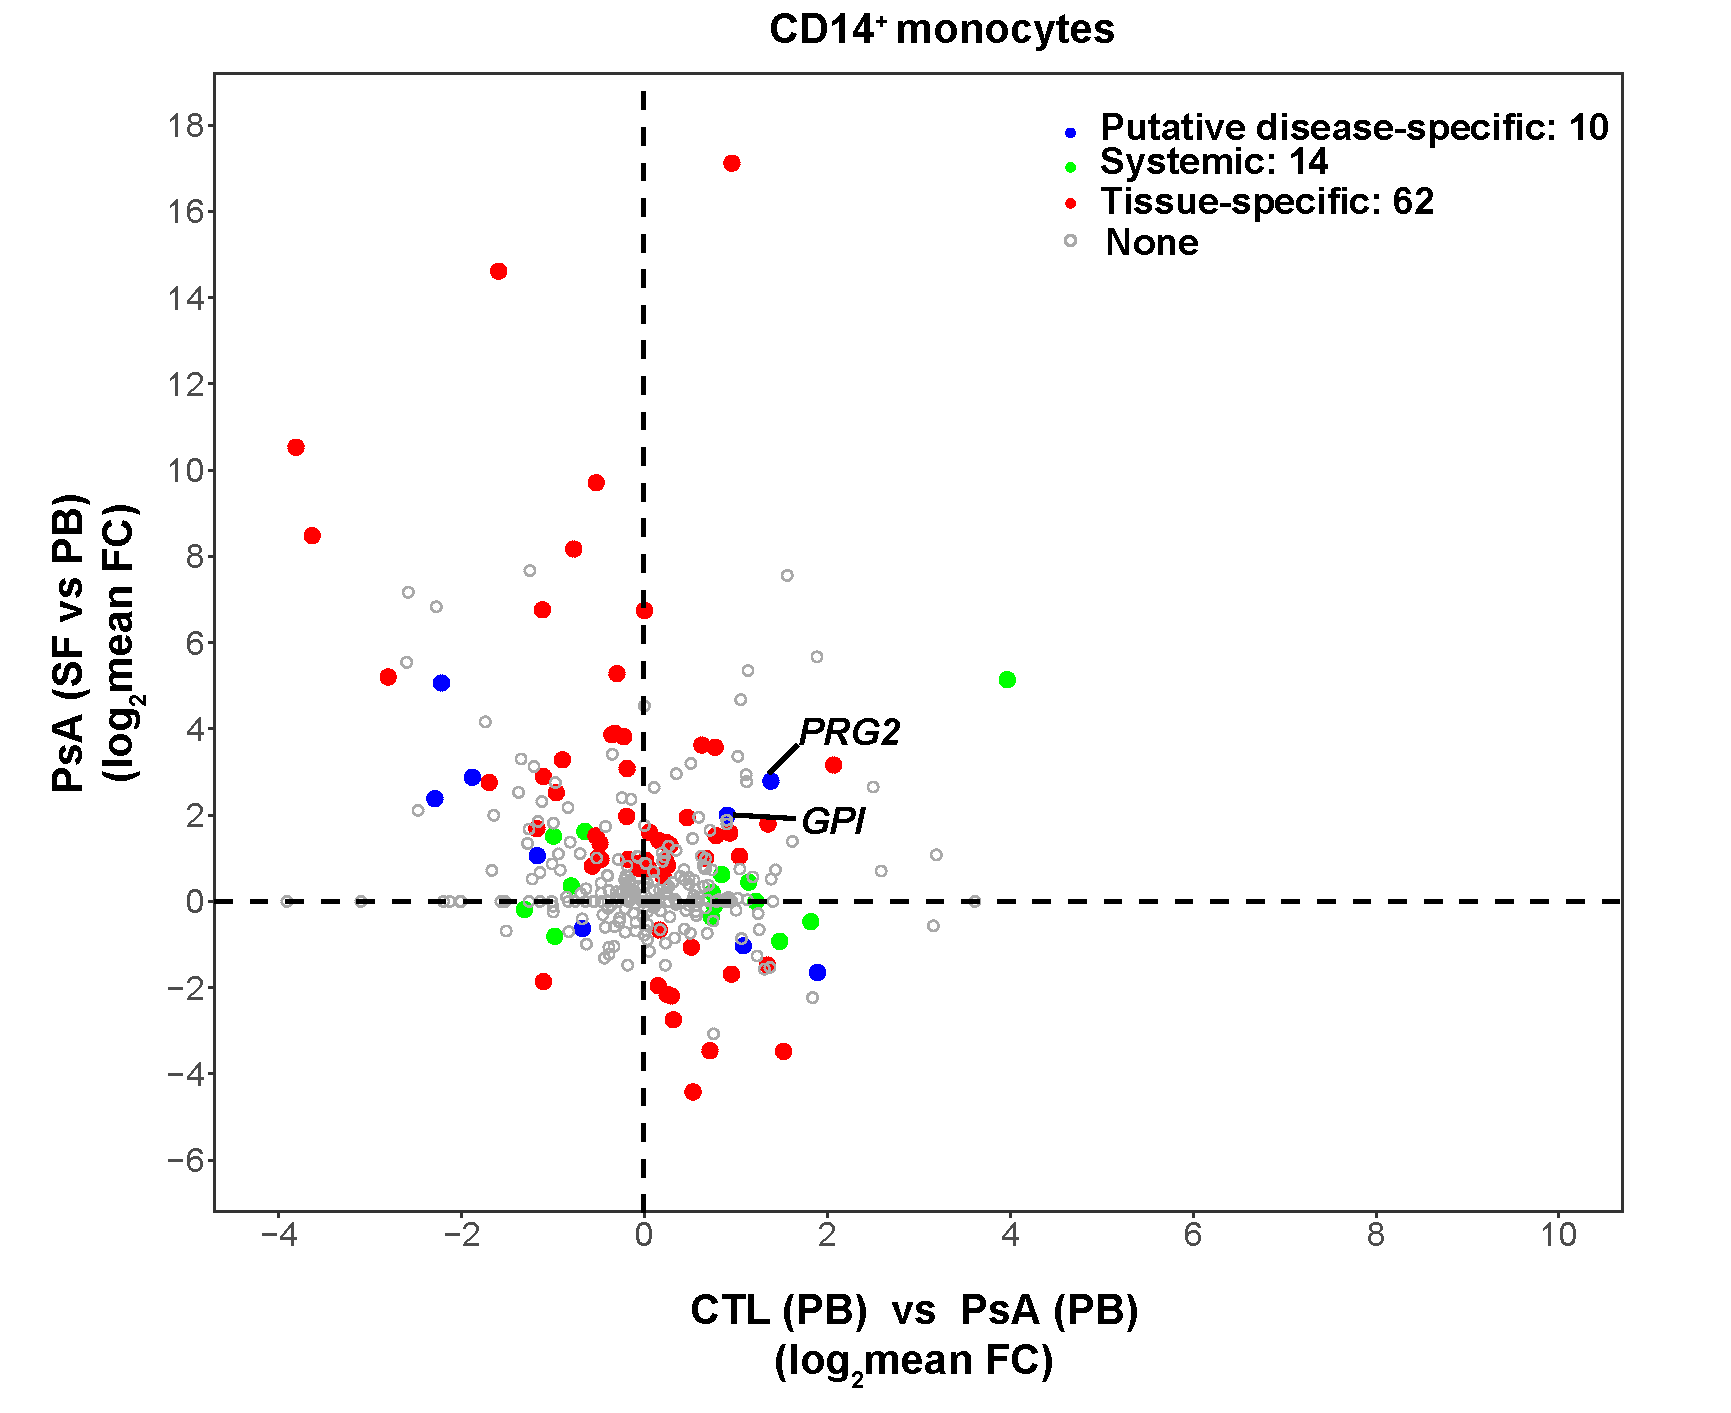
\includegraphics[width=\textwidth]{./Results3/pdfs/PSA_array_correlation_CD14_FC_HVPsA_vs_SFPBPsA}
\caption{\textbf{}}
% The percentage sign indicated that the other subfig goes side by side
\end{subfigure}%
\begin{subfigure}{0.45\textwidth}
\centering
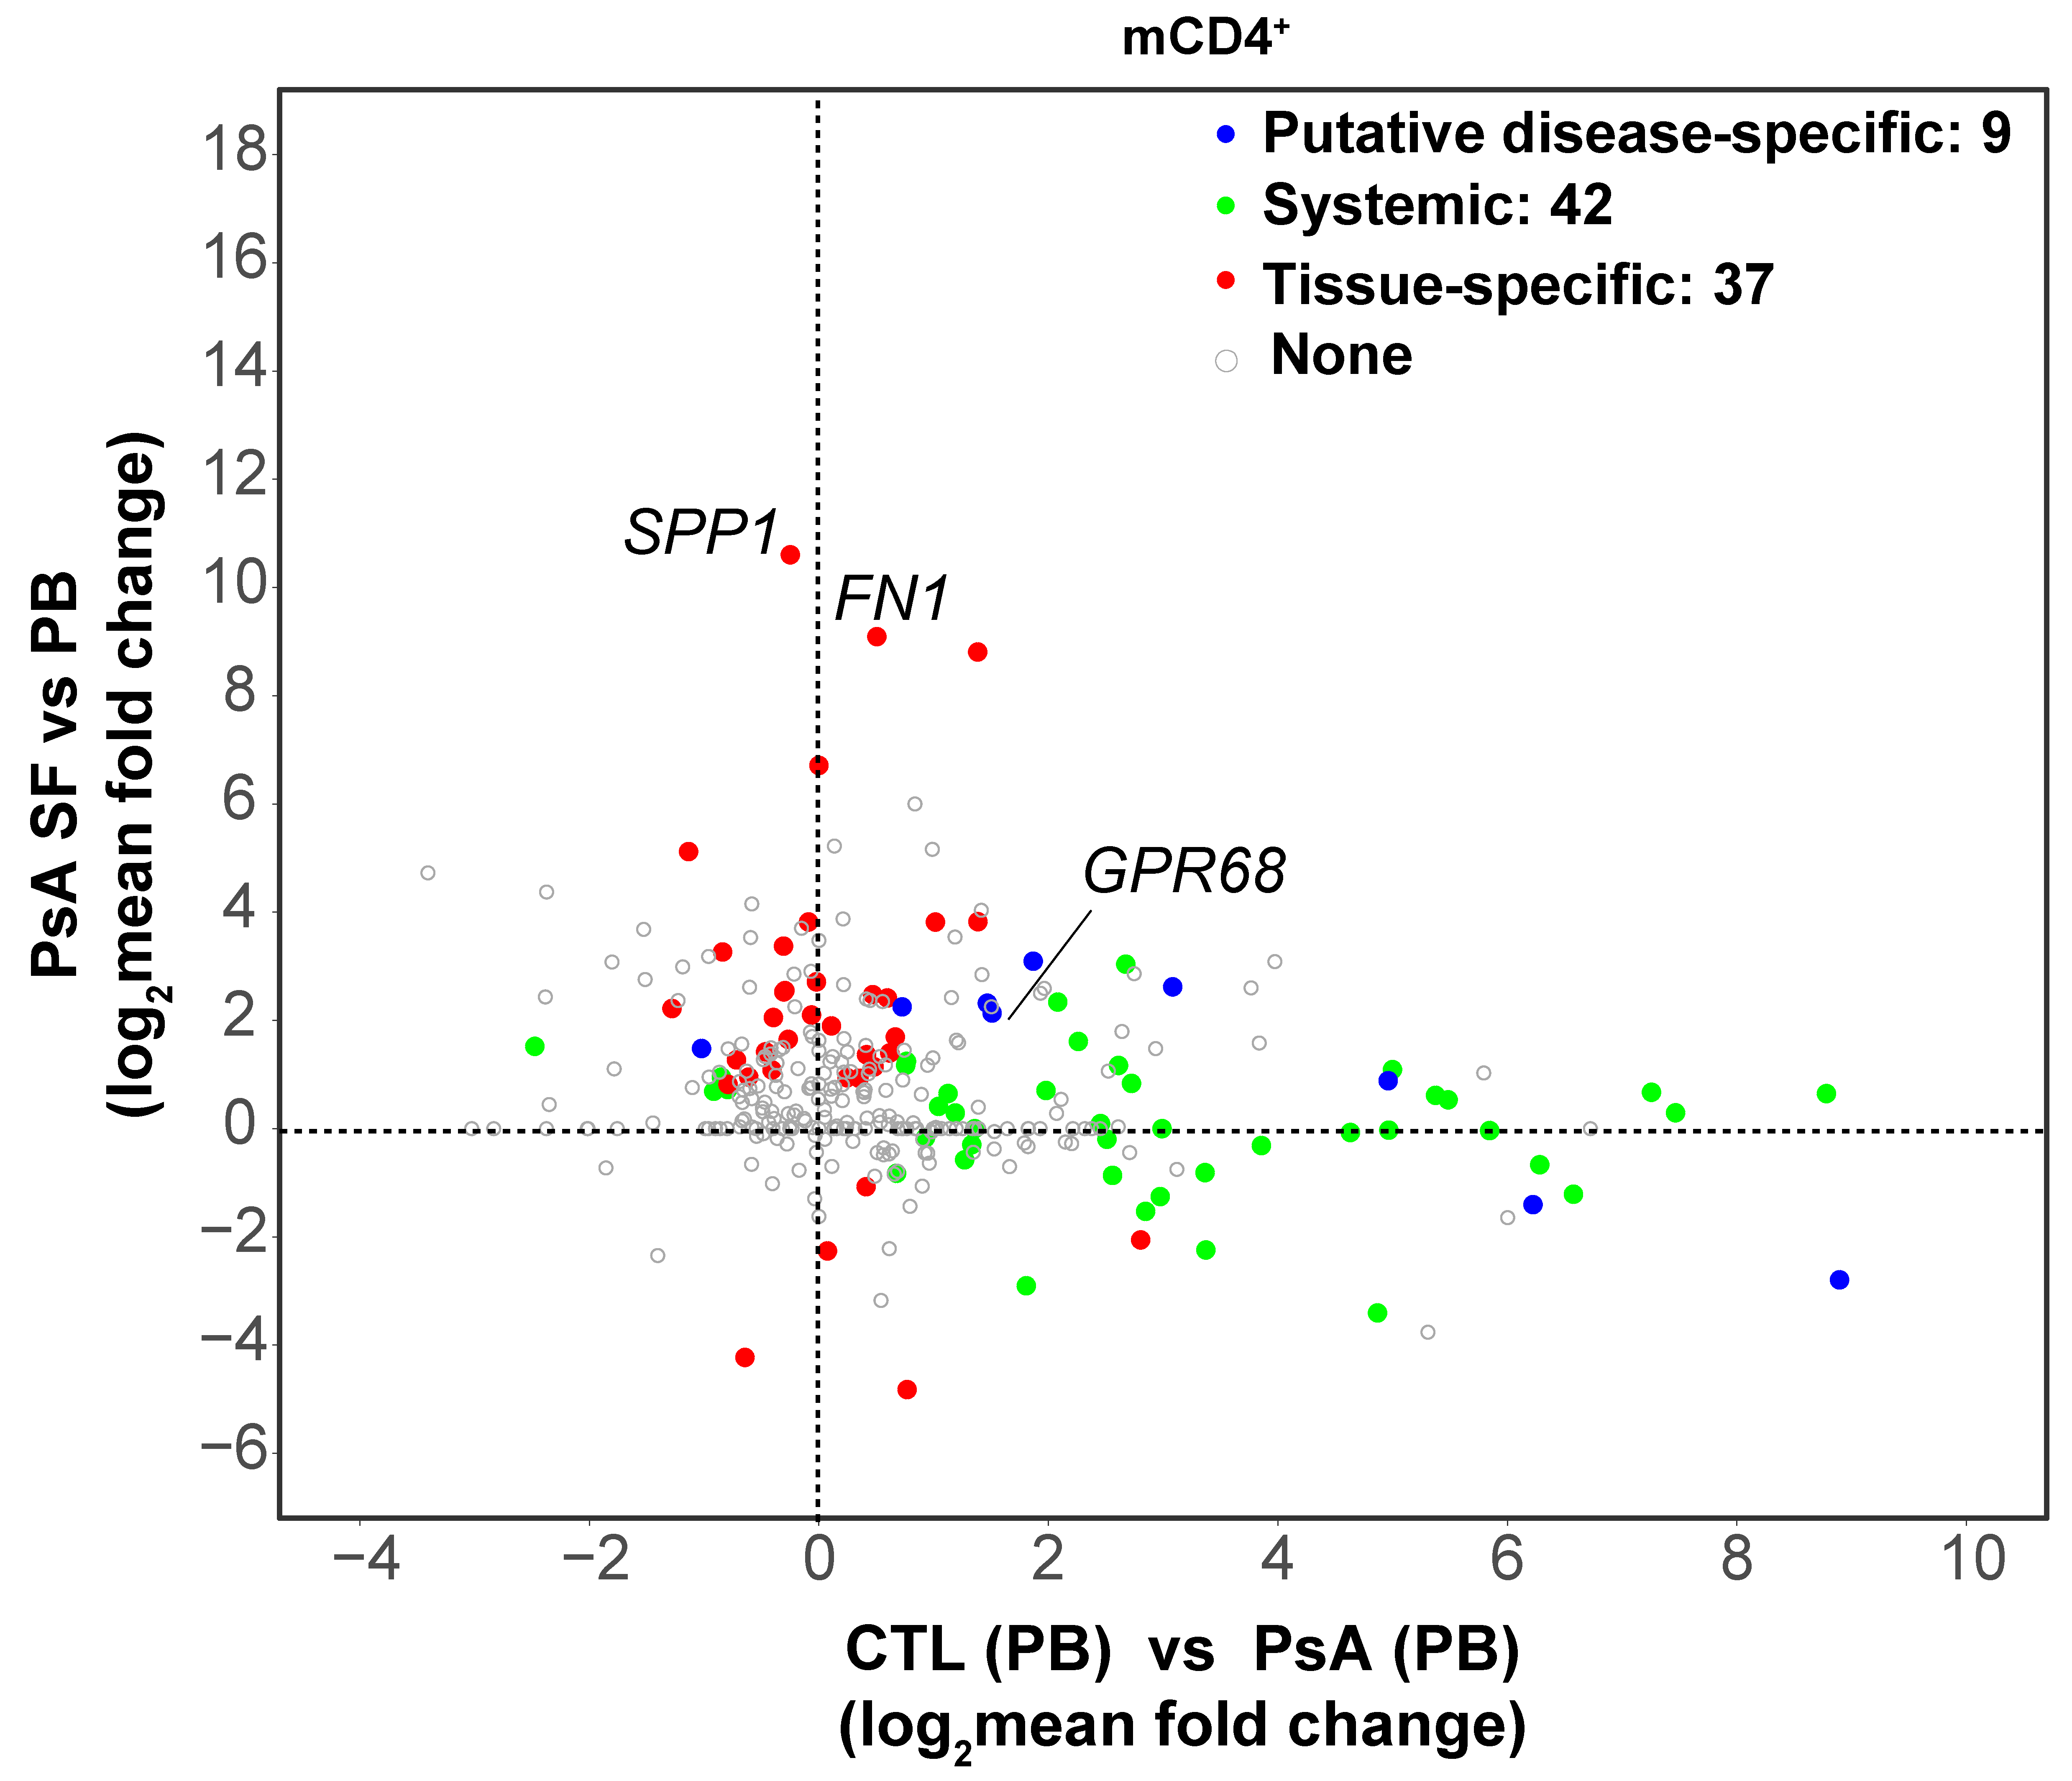
\includegraphics[width=\textwidth]{./Results3/pdfs/PSA_array_correlation_CD4_FC_HVPsA_vs_SFPBPsA}
\caption{\textbf{}}
\end{subfigure}\\
\begin{subfigure}{0.45\textwidth}
\centering
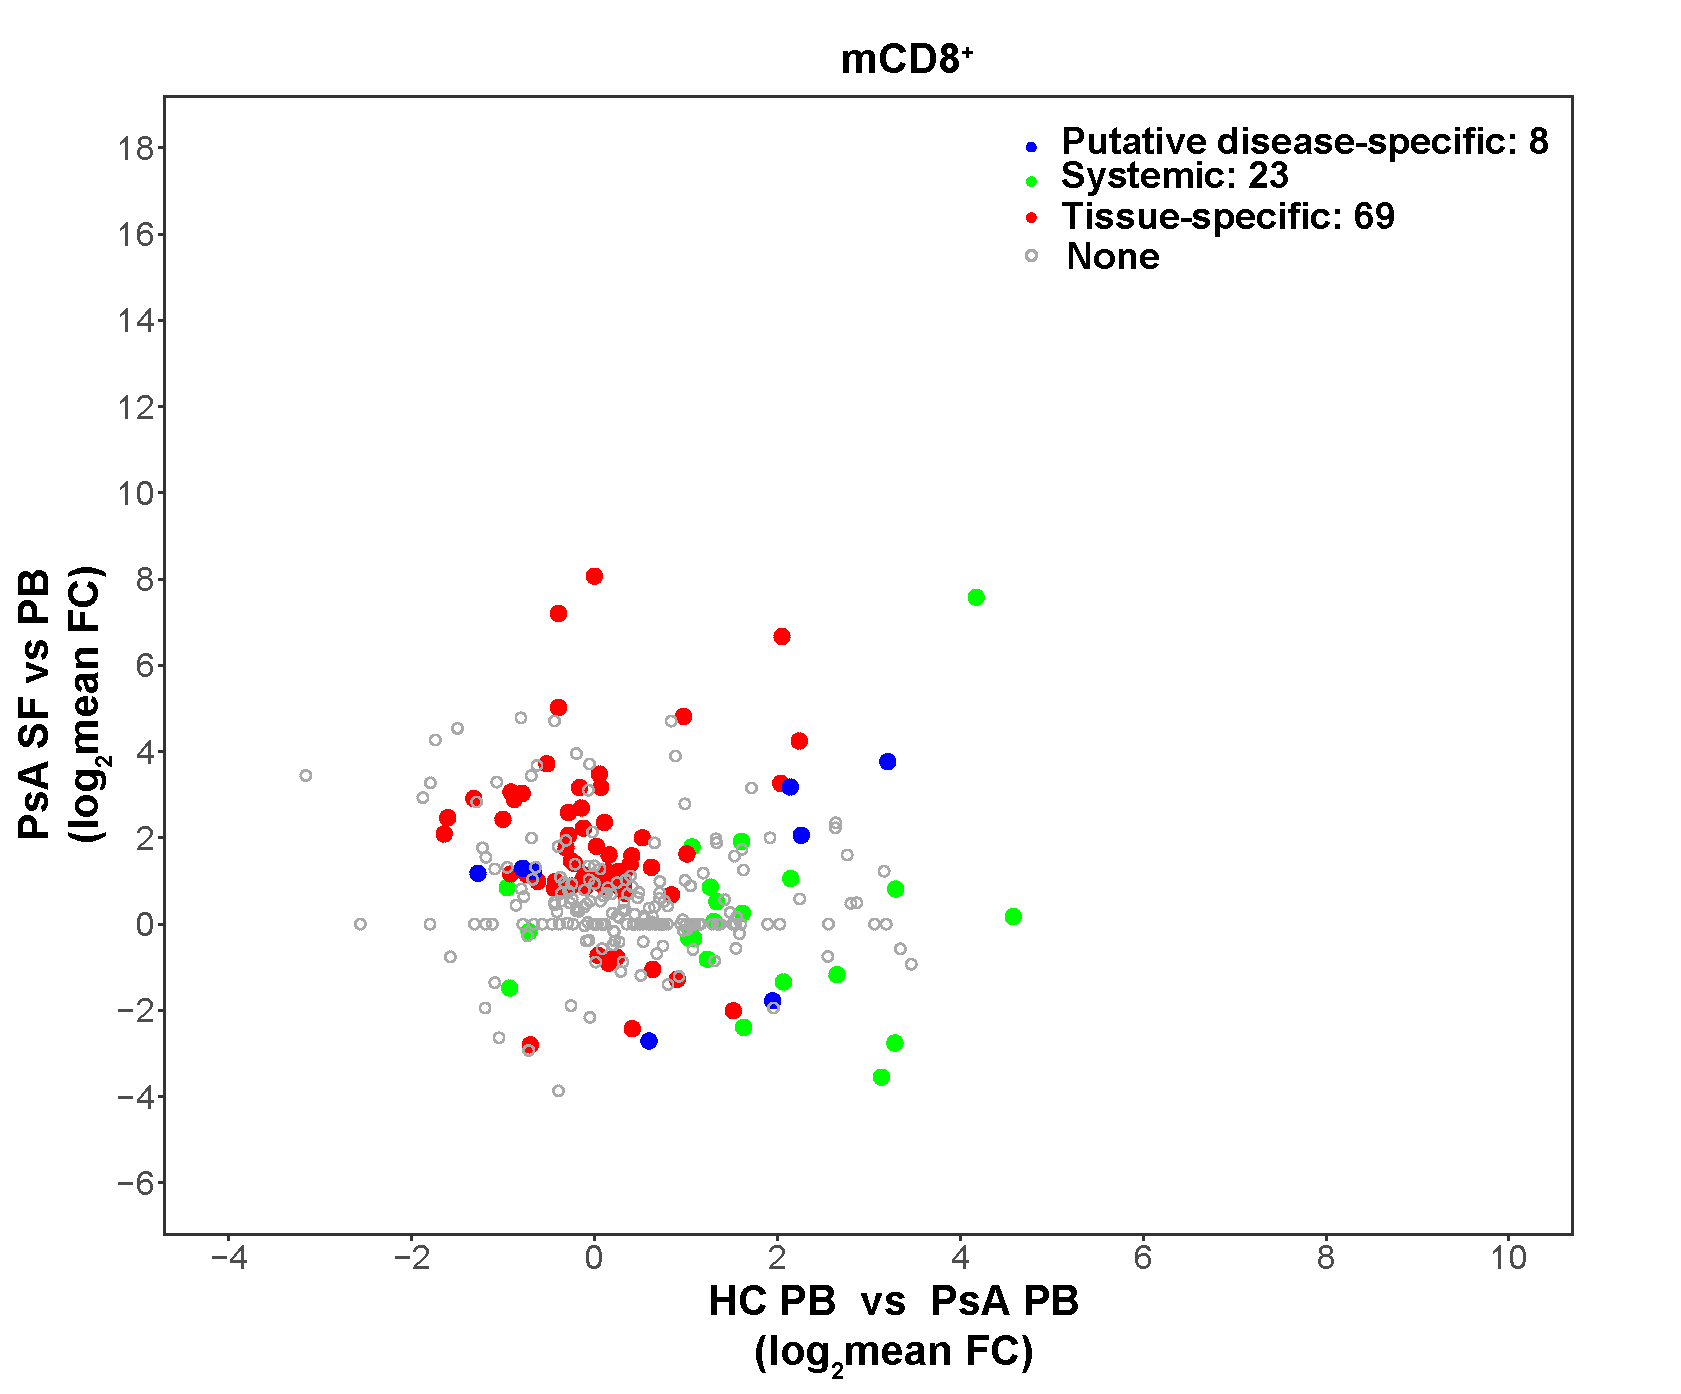
\includegraphics[width=\textwidth]{./Results3/pdfs/PSA_array_correlation_CD8_FC_HVPsA_vs_SFPBPsA}
\caption{\textbf{}}
\end{subfigure}
\caption[Comparison of immune-relevant gene expression modulation across PsA tissues (synovial fluid vs peripheral blood) and in PsA patients vs healthy controls.]{\textbf{Comparison of immune-relevant gene expression modulation across PsA tissues (synovial fluid vs peripheral blood) and in PsA patients vs healthy controls.} The qPCR log${_2}$ mean fold change for each of the genes in the PsA synovial fluid vs peripheral blood contrast are plotted against the log${_2}$ mean fold change for the same genes in the comparison peripheral blood PsA vs healthy control for (A) CD14$^+$ monocytes, (B) mCD4$^+$ and (C) mCD8$^+$ cells. The genes are colour-coded according to the three categories of genes made by comparison of changes in gene modulation between the two contrasts: systemic genes, tissue-specific and putative disease-specific. SF=synovial fluid; PB=peripheral blood. In grey genes which differential expression was not significant (p-value$<$0.05) for either of the two contrasts.}
\label{figure:PSA_PCR_array_HC_FC_correlation}
\end{figure} 



\subsubsection{Correlation between gene expression and chromatin accessibility}
% ATAC overall overlap
Overlap between differentially modulated genes (in synovial fluid vs peripheral blood) and proximal DARs was observed in the three cell types (Table \ref{tab:PSA_gene_expression_ATAC_overlap}); however was only found to be significant in CD14$^+$ monocytes (Fisher exact test p-value=0.028) and not in mCD4$^+$ and mCD8$^+$ T cells (Fisher exact test p-value=0.466 and 0.173, respectively).


\begin{table}[htbp]
%\setlength{\tabcolsep}{20pt} only to stretch the columns if you want
%\renewcommand{\arraystretch}{1.5}
\centering
\begin{tabular}{@{} c c c}
\toprule
\textbf{Cell type} & \textbf{Genes up-regulated and}        &  \textbf{Genes down-regulated and} \\
                   & \textbf{overlapping open chromatin}   &  \textbf{overlapping closed chromatin} \\
									 &	\textbf{in SF}				               &  \textbf{in SF} \\
\midrule
\midrule
          & 13 (\textit{BLNK}, \textit{CCL2$^\ast$}, \textit{CCR1$^\ast$}, \textit{CD180}, & 2 (\textit{FOS}, \textit{PROK2$^\ast$}) \\      CD14$^+$  & \textit{CXCL10}, \textit{FN1}, \textit{IL18}, \textit{IL31RA$^\ast$},    & \\
monocytes & \textit{IL7R$^\ast$}, \textit{NFKB1$^\ast$}, \textit{PRG2}, \textit{SRGAP1}, & \\
				  & \textit{STAT3}) & \\
				
\midrule
mCD4$^+$ & 3 (\textit{CXCL13}, \textit{CXCR6$^\ast$}, \textit{IL2RA}) & 0 \\

\midrule
mCD8$^+$ & 6 (\textit{CCL3}, \textit{CCR2}, \textit{CCR5} ,\textit{IRF4} & 1 (\textit{EPHX2}) \\
         & \textit{TNFSF10}, \textit{YARS}) & \\

\bottomrule
\end{tabular}
\medskip %gap
\caption[Immune genes with significant modulated expression in synovial fluid and proximal to a DAR in ATAC.]{\textbf{Immune genes with significant modulated expression in synovial fluid and proximal to a DAR in ATAC.} An overlap is defined by significant change in expression (p-value$<$0.05) of a particular gene where there is also a proximal DAR showing changes in chromatin accessibility in the same direction. $^\ast$ indicates that the proximal DAR overlapping an eRNA identified by FANTOM5 project in that particular cell type (see subsection Characterisation of the differential accessible chromatin regions). SF=synovial fluid.}
\label{tab:PSA_gene_expression_ATAC_overlap}
\end{table}

In CD14$^+$ monocytes, 13 out of the 56 significantly up-regulated genes in synovial fluid were also found to be proximal to a synovial fluid open DARs. One example being \textit{IL7R}, where its increased expression in synovial fluid correlated with increased chromatin accessibility at the 5' and 3' UTR of this gene (Figure \ref{figure:PsA_FAST_ATAC_gene_boy_DOCS_CD14_NK}B). Another relevant example was the \textit{FN1} gene, for which up-regulated expression in synovial biopsies compared to peripheral blood has been previously reported \parencite{Dolcino2015}. In this cohort, \textit{FN1} expression was up-regulated in synovial fluid for all three cell types, with the highest fold change found in CD14$^+$ monocytes (Figure \ref{figure:PSA_PCR_array_vulcano_plots}A), concomitantly with more accessible chromatin at the promoter and downstream the 3' UTR of the gene (Figure \ref{figure:PSA_CD14_ATAC_FN1}). 
%Lesser overlap between up-regulated gene expression and open chromatin in synovial fluid compared to peripheral blood was observed in mCD4$^+$ and mCD8$^+$ (6 and 3 hits, respectively). Only CD14$^+$ monocytes and mCD8$^+$ cells presented overlap between synovial fluid down-regulated genes and proximal less accessible in synovial fluid (2 and 1, respectively). Notably, none or very few genes presented opposite direction of change in gene expression and chromatin accessibility on a proximal DAR (4 in CD14$^+$ monocytes, 0 in mCD4$^+$ and 2 in mCD8$^+$), reinforcing the biological relevance of the observed overlaps. 
%decide which example to use: I have included IL7R in monocytes and maybe could use FN1 to complete
	%Example expression in CD14 FOS,FN1,CCL2,CXCL10
	
\begin{figure}[htbp]
\centering
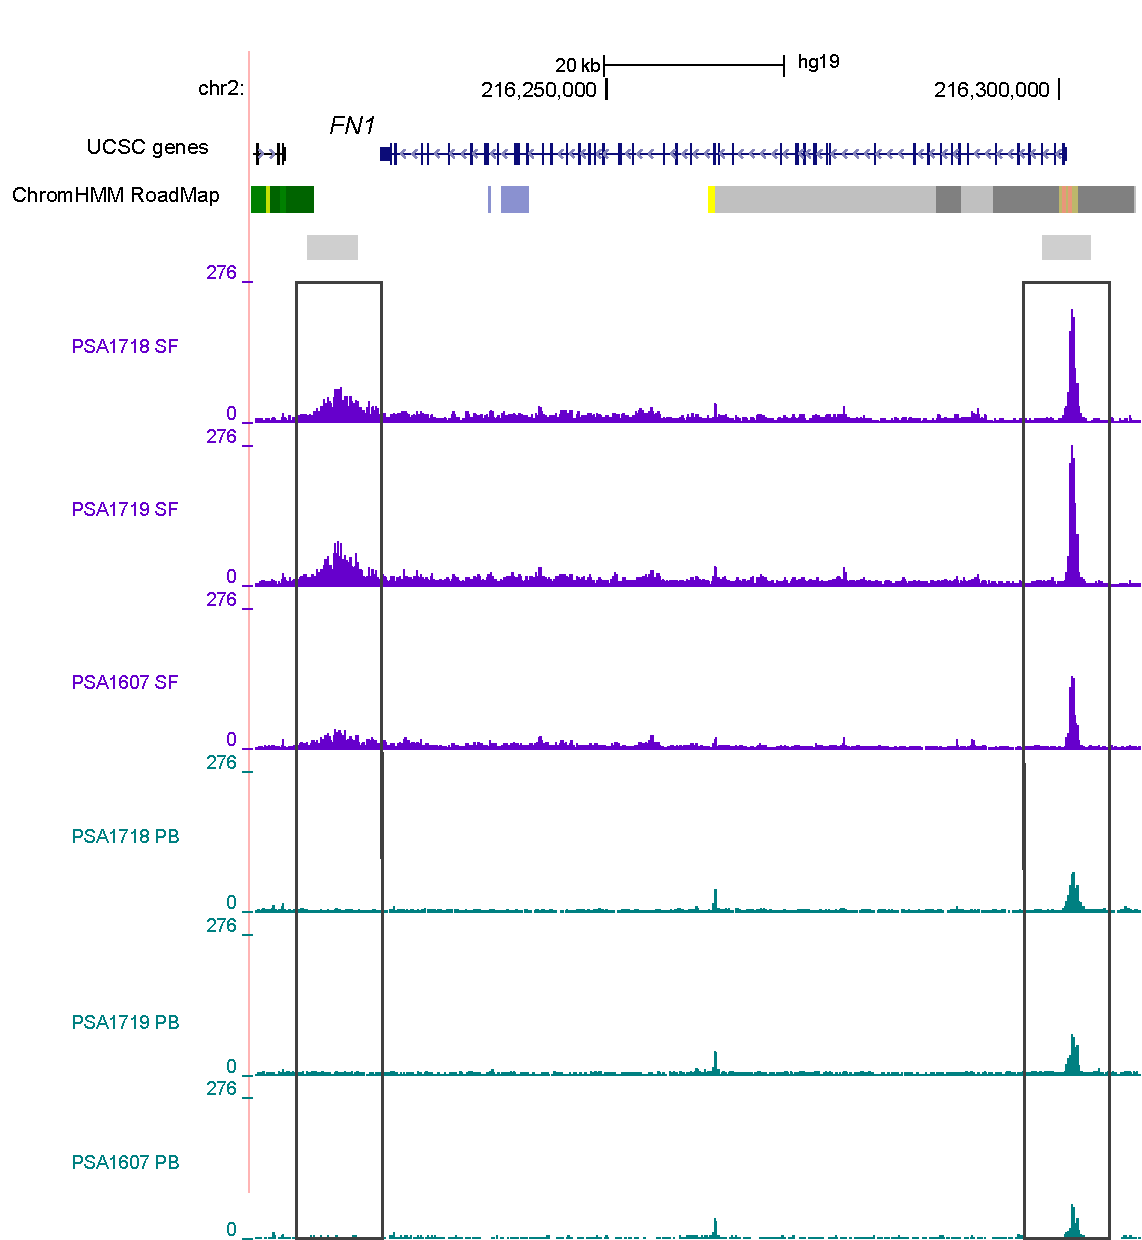
\includegraphics[width=0.6\textwidth]{./Results3/pdfs/PSA_CD14_ATAC_FN1_paired_gene_expression}
\caption[Chromatin accessibility landscape at the qPCR differentially expressed \textit{FN1} gene in CD14$^+$ monocytes.]{\textbf{Chromatin accessibility landscape at the qPCR differentially expressed \textit{FN1} gene in CD14$^+$ monocytes.} UCSC Genome Browser view illustrating the ATAC normalised read density (y-axis) in two DARs located at the promoter and downstream the 3' UTR of the \textit{FN1} gene (x-axis) in CD14$^+$ monocytes from synovial fluid and peripheral blood in 3 PsA patients. Both DARs were more accessible in synovial fluid when compared to peripheral blood. Tracks are colour-coded by tissue (SF=purple and PB=turquoise). The Roadmap Epigenomics Project chromatin segmentation track for peripheral blood isolated CD14$^+$ monocytes is also shown. All DARs were significant based on FDR$<$0.01 and fold change$>$1.5. SF=synovial fluid; PB=peripheral blood.}
\label{figure:PSA_CD14_ATAC_FN1}
\end{figure}



\subsubsection{Pathway enrichment analysis highlights the role of synovial CD14$^+$ monocytes in cytokine and chemokine production}
%Describe pathway analysis results and curate the pathway of interest
To identify relevant pathways amongst the modulated genes between synovial fluid and peripheral blood, enrichment analysis was performed for each individual cell type. Up-regulated and down-regulated genes showing mean fold change$>$1.5 and p-value$<$0.05 were used as input for the enrichment analysis. Interestingly, the modulated genes between synovial fluid and peripheral blood in CD14$^+$ monocytes were significantly enriched (FDR$<$0.05) for chemokine, NOD-like signalling and TLR signalling pathways (Table \ref{table:PSA_PCR_array_pathway_analysis}). Significant enrichment was also found for ``Innate immune system'' and ``Neutrophil degranulation'' pathways. Of particular relevance in monocytes were the chemokine, NOD-like and TLR signalling pathways, involved in the activation of cytokines and chemokines gene expression, leading to T cell recruitment and perpetuation of the adaptive inflammatory response. Some of the genes, such as \textit{CCL5} and \textit{NFKB}, contributed to the enrichment of these three relevant pathways.

The TLR signalling pathways enrichment involved \textit{FN1} and \textit{SPP1}, two of the top differentially expressed genes found in this pilot study, and up-regulation of the TLR receptors \textit{TLR1} and \textit{TLR2} (Table \ref{table:PSA_PCR_array_pathway_analysis}). Similarly to \textit{FN1}, \textit{SPP1} was also highly up-regulated (mean fold change$>$16) in the three cell types but showed the greatest fold change in CD14$^+$ monocytes (Figure \ref{figure:PSA_PCR_array_vulcano_plots}A).Genes such as \textit{TNF}, \textit{IRF7} and \textit{MYD88} particularly highlighted the cross-link between the NOD-like and the TLR signalling pathways. 

%Accordingly, the enrichment of synovial fluid open DARs in CD14$^+$ monocytes for the NF$\kappa$B pathway is closely related to the enrichment for TLR and NOD-like signalling pathways at the transcriptomic level, since both pathways lead to the activation of the NF$\kappa$B TF  (Figure \ref{figure:PSA_ATAC_pathway_analysis_all_DOC} a). %Both, TLR and NOD-like pathways lead to the activation of the NF$\kappa$B TF, which induces transcriptional activation of pro-inflammatory cytokines, further supported by the enrichment of synovial fluid open DARs in the proximity of genes from the IL-2, IL-3, IL-5 and GM-Csynovial fluid pathways (Figure \ref{figure:PSA_ATAC_pathway_analysis_all_DOC} a). Moreover, the pivotal role of NF$\kappa$B in the immune transcriptional profile of synovial fluid CD14$^+$ monocytes is additionally sustained at the chromatin accessibility level by the enrichment of synovial fluid accessible chromatin sites for this TF (Figure \ref{figure:PSA_TFBS}).  

The enrichment for the chemokine pathway in CD14$^+$ monocytes (Table \ref{table:PSA_PCR_array_pathway_analysis}) included genes highly up-regulated (mean fold change$>$16) in synovial fluid compared to peripheral blood (e.g \textit{CCL18} and \textit{CCL2}) for all three cell types (Figure \ref{figure:PSA_PCR_array_vulcano_plots}) as well as genes only consistently modulated between synovial fluid and peripheral blood in CD14$^+$ monocytes (e.g \textit{CCL28}, Figure \ref{figure:PSA_PCR_array_5_pcnt_heatmap}). %The chemokine pathway includes production of chemotractant molecules involved in the recruitment of leukocytes to the site of inflammation and reactive oxygen species (ROS) through Ca$^2$$^+$ mobilisation, a pathway that has previously presented to be enriched in synovial fluid open DARs in CD14$^+$ monocytes (Figure \ref{figure:PSA_ATAC_pathway_analysis_all_DOC} a).

The modulated genes between synovial fluid and peripheral blood in mCD4$^+$ T cells only showed significant enrichment for genes in the IL-10 signalling pathway (Table \ref{table:PSA_PCR_array_pathway_analysis}), whereas mCD8$^+$ modulated genes between the two tissues were not enriched for any pathway.



\begin{landscape}
\begin{center}
\begin{longtable}[ht]{c c c }
\caption[Pathway enrichment analysis for the modulated genes between synovial fluid and peripheral blood in CD14$^+$ and mCD4$^+$.]{\textbf{Pathway enrichment analysis for the modulated genes between synovial fluid and peripheral blood in CD14$^+$ and mCD4$^+$.} The analysis was performed using only those genes showing p-value$<$0.05 and mean fold change$>$1.5. Reported enriched pathways were significant at an FDR $<$0.05 and fold change is specified in brackets.}
\label{table:PSA_PCR_array_pathway_analysis} \\
\toprule
\textbf{Cell type} & \textbf{Pathway} & \textbf{Genes} \\						
\midrule
\midrule
\textbf{CD14$^+$} & Chemokine signalling & \textit{CCL17}, \textit{CCL18}, \textit{CCL2}, \textit{CCL28}, \textit{CCL5}, \textit{CCL7}, \textit{CCR1}, \textit{CCR5},\textit{CXCL10} \\  
									& \textit{(fold change=1.53)}   & \textit{CXCL12}, \textit{CXCL16}, \textit{CXCL5}, \textit{CXCL9}, \textit{NFKB1}, \textit{PPBP}, \textit{PF4V1}, \textit{STAT3}, \textit{XCR1}\\
									
									& NOD-like receptor signalling & \textit{CCL2}, \textit{CCL5}, \textit{IFNAR1}, \textit{IL18}, \textit{IRF7}, \textit{MEFV}, \textit{MYD88}, \textit{NFKB1}, \\
								  & \textit{(fold change=1.85)}           & \textit{NAMPT}, \textit{TNF} \\

									& TLR signalling       & \textit{CCL5}, \textit{CXCL10}, \textit{CXCL9}, \textit{IFNAR1}, \textit{IRF7}, \textit{MYD88}, \textit{NFKB1}, \textit{SPP1},\textit{FOS},\\ 
								  & \textit{(fold change=1.64)}  & \textit{TLR1}, \textit{TLR2}, \textit{TLR8}, \textit{TNF}\\

\midrule
\textbf{mCD4$^+$} & IL-10 signaling & \textit{CCL3}, \textit{CCL4}, \textit{CCL5}, \textit{CCR1}, \textit{CCR2}, \textit{CSF1}, \textit{CSF3}, \textit{IL10RA}, \\
									& \textit{(fold change=2.13)} & \textit{IL1R1}, \textit{IL1R2}\\
\bottomrule
\medskip
\end{longtable}
\end{center}
\end{landscape}

Pathway analysis using the significantly modulated genes between peripheral blood of healthy controls and PsA patients only showed significant enrichment for the Reactome immune system pathway in CD14$^+$ monocytes and mCD4$^+$ cells. This suggests some tissue-specificity of the pathways enriched for DEGs between synovial fluid and peripheral blood in this analysis, highlighting a more pronounced inflammatory phenotype of the pathological CD14$^+$ monocytes at the inflamed joints.


%In addition to pathway enrichment, network analysis was performed to understand the interaction and relationship of the differentially expressed genes between synovial fluid and peripheral blood. A gene subnetwork was identified from the STRING functional interaction database using as input all the genes from the qPCR array (regardless of p-value significance and fold change) and ranked them based on the best p-value across the 3 analysed cell types. The identified subnetwork predominantly included significantly modulated genes between synovial fluid and peripheral blood in at least one of the cell types. Amongst the most interesting nodes was the single Ig and Toll-interleukine domain containing gene (\textit{SIGIRR}), which is a negative regulator of the TLR signalling pathway (Figure \ref{figure:PSA_PCR_network_analysis}). \textit{SIGIRR} was significantly down-regulated in synovial fluid CD14$^+$ monocytes, consistent with the significant up-regulation (p-value$<$0.05) of the \textit{TLR1}, \textit{TLR2}, \textit{MYD88} genes in synovial fluid as well as the enrichment for the TLR pathway in this cell type (Figure \ref{figure:PSA_PCR_array_5_pcnt_heatmap} and \ref{table:PSA_PCR_array_pathway_analysis}). Moreover, the significant up-regulation of \textit{NFKB} and \textit{TNF} in the synovial fluid CD14$^+$ monocytes appeared as a downstream result of the functional connection with TLR pathway members such as \textit{MyD88}. Conversely, in mCD4$^+$ and mCD8$^+$ the modulation of these members did not appear to be significant between synovial fluid and peripheral blood.% however, in mCD8$^+$, \textit{TNF} expression is also significantly up-regulated in the synovium compared to PB. 

%%SIGIRR down-reg https://www.ncbi.nlm.nih.gov/pmc/articles/PMC2996602/

%Another interesting part of the network is the connection of the TLR pathway and the chemokine production through \textit{NF$\kappa$B}, \textit{TNF} and \textit{CCL2} (Figure \ref{figure:PSA_PCR_network_analysis}). \textit{CCL2} is connected to \textit{CXCL10} and subsequently with \textit{CCL18} and \textit{CCR5}; chemokines and chemokine receptors regulating migration and infiltration of monocytes and memory T cells at the sites of inflammation. This network analysis also highlighted relationship between \textit{IL7R} and \textit{IL2RG} coding for the two chains of the IL-7R. %Interestingly, these two nodes were only significantly up-regulated in synovial fluid CD14$^+$ monocytes when compared to PB, supporting the novel cell and context specific role of IL-7R and IL-7R polymorphism under inflammatory conditions in CD14$^+$ monocytes\parencite{Al-Mossawi2018}.

% I could also talk about the FOS, PROK2 and PTGS2

%\begin{figure}[htbp]
%\centering
%\includegraphics[width=\textwidth]{./Results3/pdfs/PSA_PCR_array_network_analysis}
%\caption[Protein network analysis based on the immune qPCR array expression data.]{\textbf{Protein network analysis based on the immune qPCR array expression data.} STRING interaction network (including known and predicted protein–protein interactions) was used to superpose all the genes quantified in the qPCR array ranked by the best p-value across the cell types and to obtain a 30 gene size subnetwork, common for all three cell types. This network included maximal number of significant genes (p-value$<$0.05) in at least one cell type and minimal presence of non-significant genes as linkers in the network. In the left hand panel, for each cell type each of the nodes (proteins) of the identified subnetwork (the same for each cell type, as previously explained) are colour-coded by the change of expression (log${_2}$ mean fold change) for the corresponding gene in the qPCR analysis. On the right hand panel, each of the nodes in the same subnetwork are colour-coded by the level of significance (p-value) for the reported modulation in gene expression (log${_2}$ mean fold change) in the qPCR array.}
%\label{figure:PSA_PCR_network_analysis}
%\end{figure}




Overall, the integration of the chromatin accessibility and immune transcriptional data reinforced a relevant role of synovial CD14$^+$ monocytes in the production of cytokines and chemokines, likely leading to activation of the innate immune response and the recruitment of T cells to this site of inflammation. 


%\subsubsection{Tissue and disease specificity in gene expression modulation and relevant biological pathways}
%
%In order to better understand the disease and tissue specificity of the prior transcriptomic results, gene expression was analysed in CD14$^+$ monocytes, mCD4$^+$ and mCD8$^+$ isolated from peripheral blood in three healthy controls using the same qPCR array. In each of the cell types, the fold change in was calculated for the mean peripheral blood expression across the three PsA patients compared to the mean expression of the three healthy controls (as detailed in Chapter \ref{ch:Mat}). Similar to the previous analysis, pvals for the fold change significance were calculated for each particular genes. Integration of the previous results of modulated gene expression between synovial fluid and peripheral blood in PsA (see Immune-relevant gene expression by qPCR) with this analysis allowed the identification of three group of genes (Figure \ref{figure:PSA_PCR_array_HC_FC_correlation}). First, the genes only significantly modulated (based on p-value and fold change threshold criteria) in peripheral blood between controls and PsA were designated as systemic genes (Figure \ref{figure:PSA_PCR_array_HC_FC_correlation} green dots). Those genes were not significantly modulated in the prior analysis comparing synovial fluid versus peripheral blood within PsA patients and could then be considered as the circulating disease "footprint". In this respect, CD14$^+$ monocytes was the cell type with lower number of systemic modulated genes (14), compared to mCD8$^+$ (23) and mCD4$^+$ (42) (Figure \ref{figure:PSA_PCR_array_HC_FC_correlation}a, b and c). Amongst these genes were \textit{CCL24} and \textit{CCL27} in CD14$^+$ monocytes, \textit{CCR7} and \textit{TLR4} in mCD4$^+$ cells and \textit{CCR10} in mCD8$^+$ cells.  
%
%
%\begin{figure}[htbp]
%\centering
%\begin{subfigure}{0.45\textwidth}
%\centering
%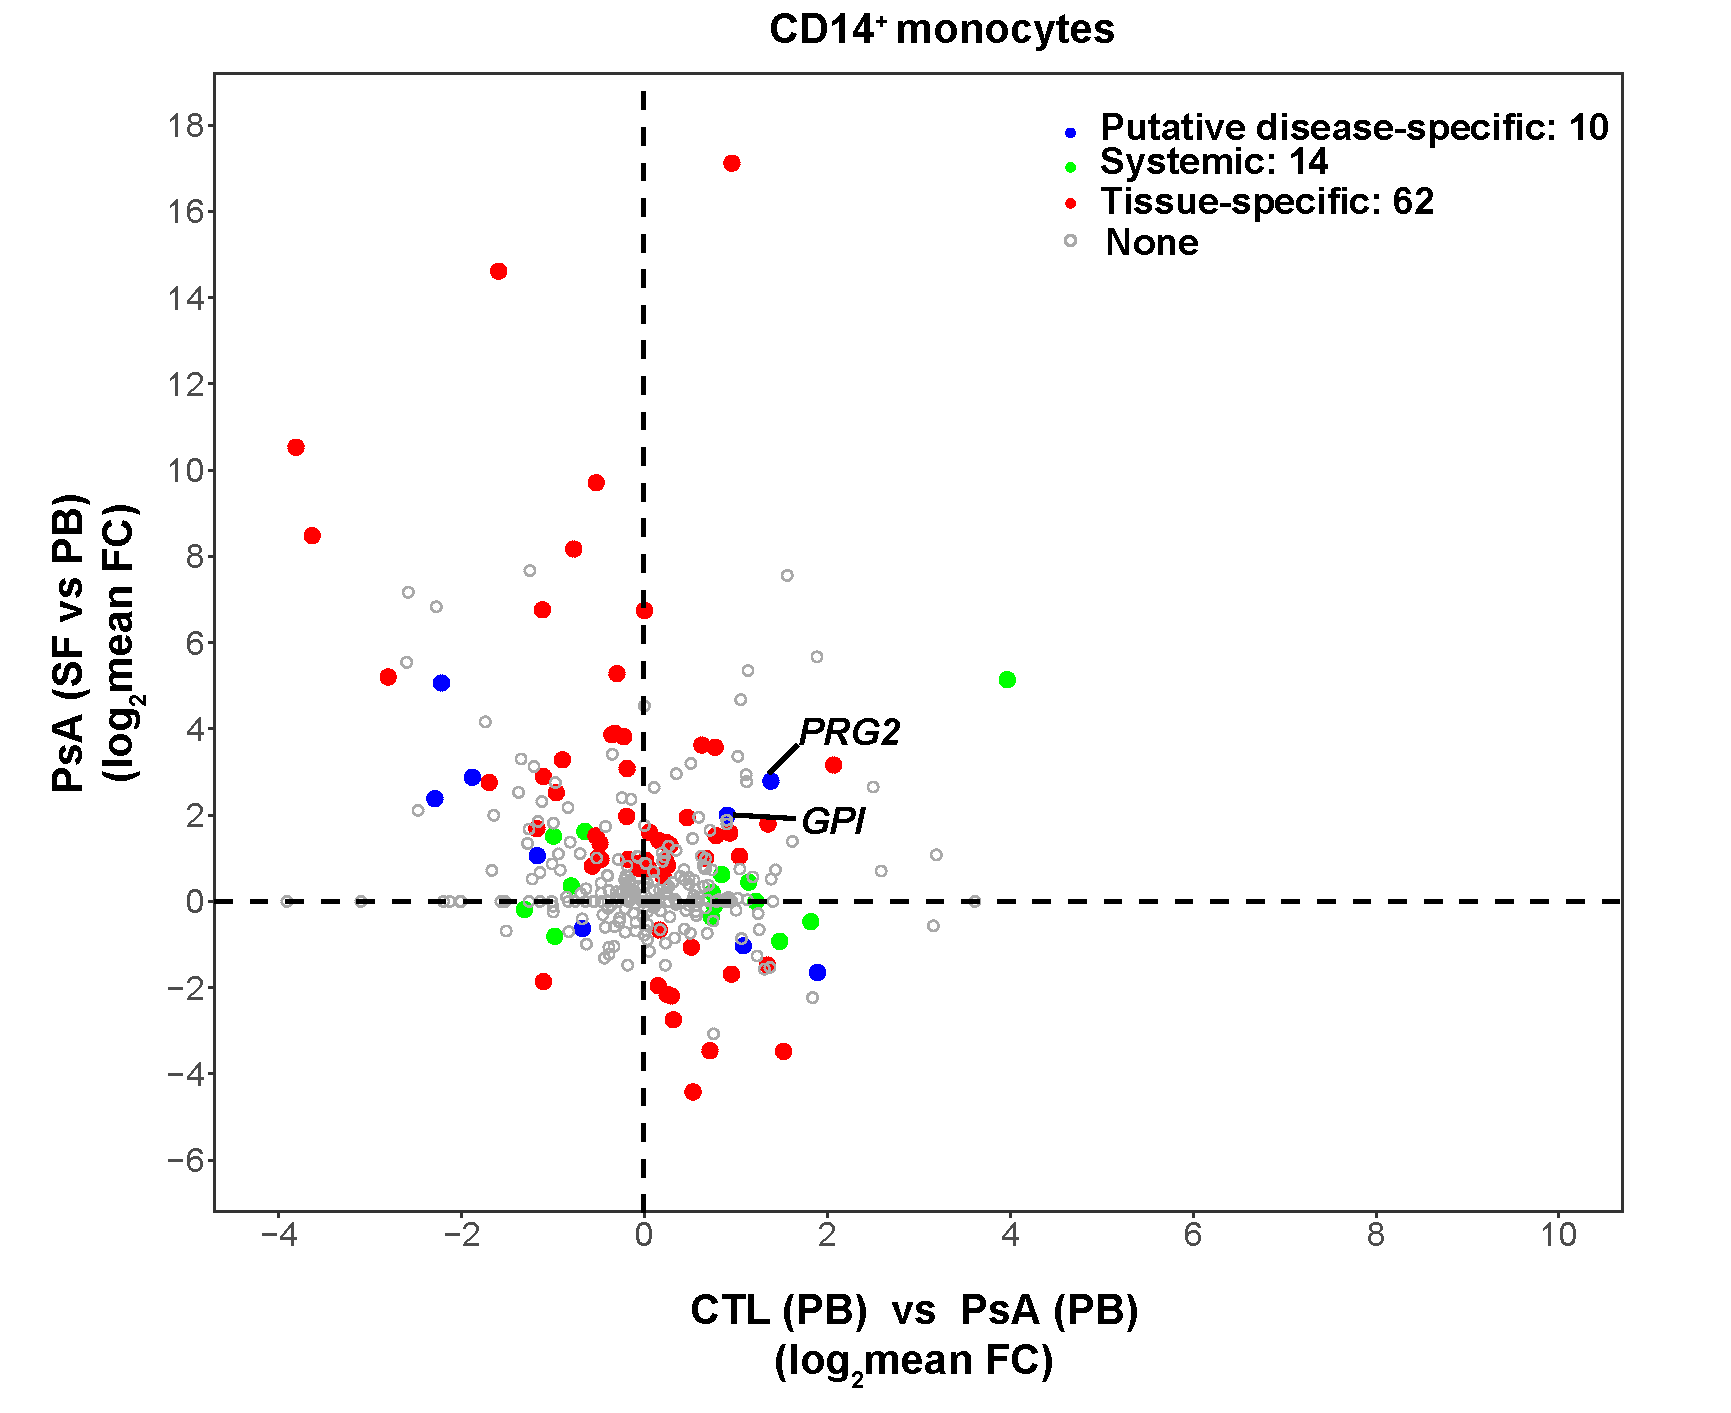
\includegraphics[width=\textwidth]{./Results3/pdfs/PSA_array_correlation_CD14_FC_HVPsA_vs_SFPBPsA}
%\caption{\textbf{}}
%% The percentage sign indicated that the other subfig goes side by side
%\end{subfigure} \\
%\begin{subfigure}{0.45\textwidth}
%\centering
%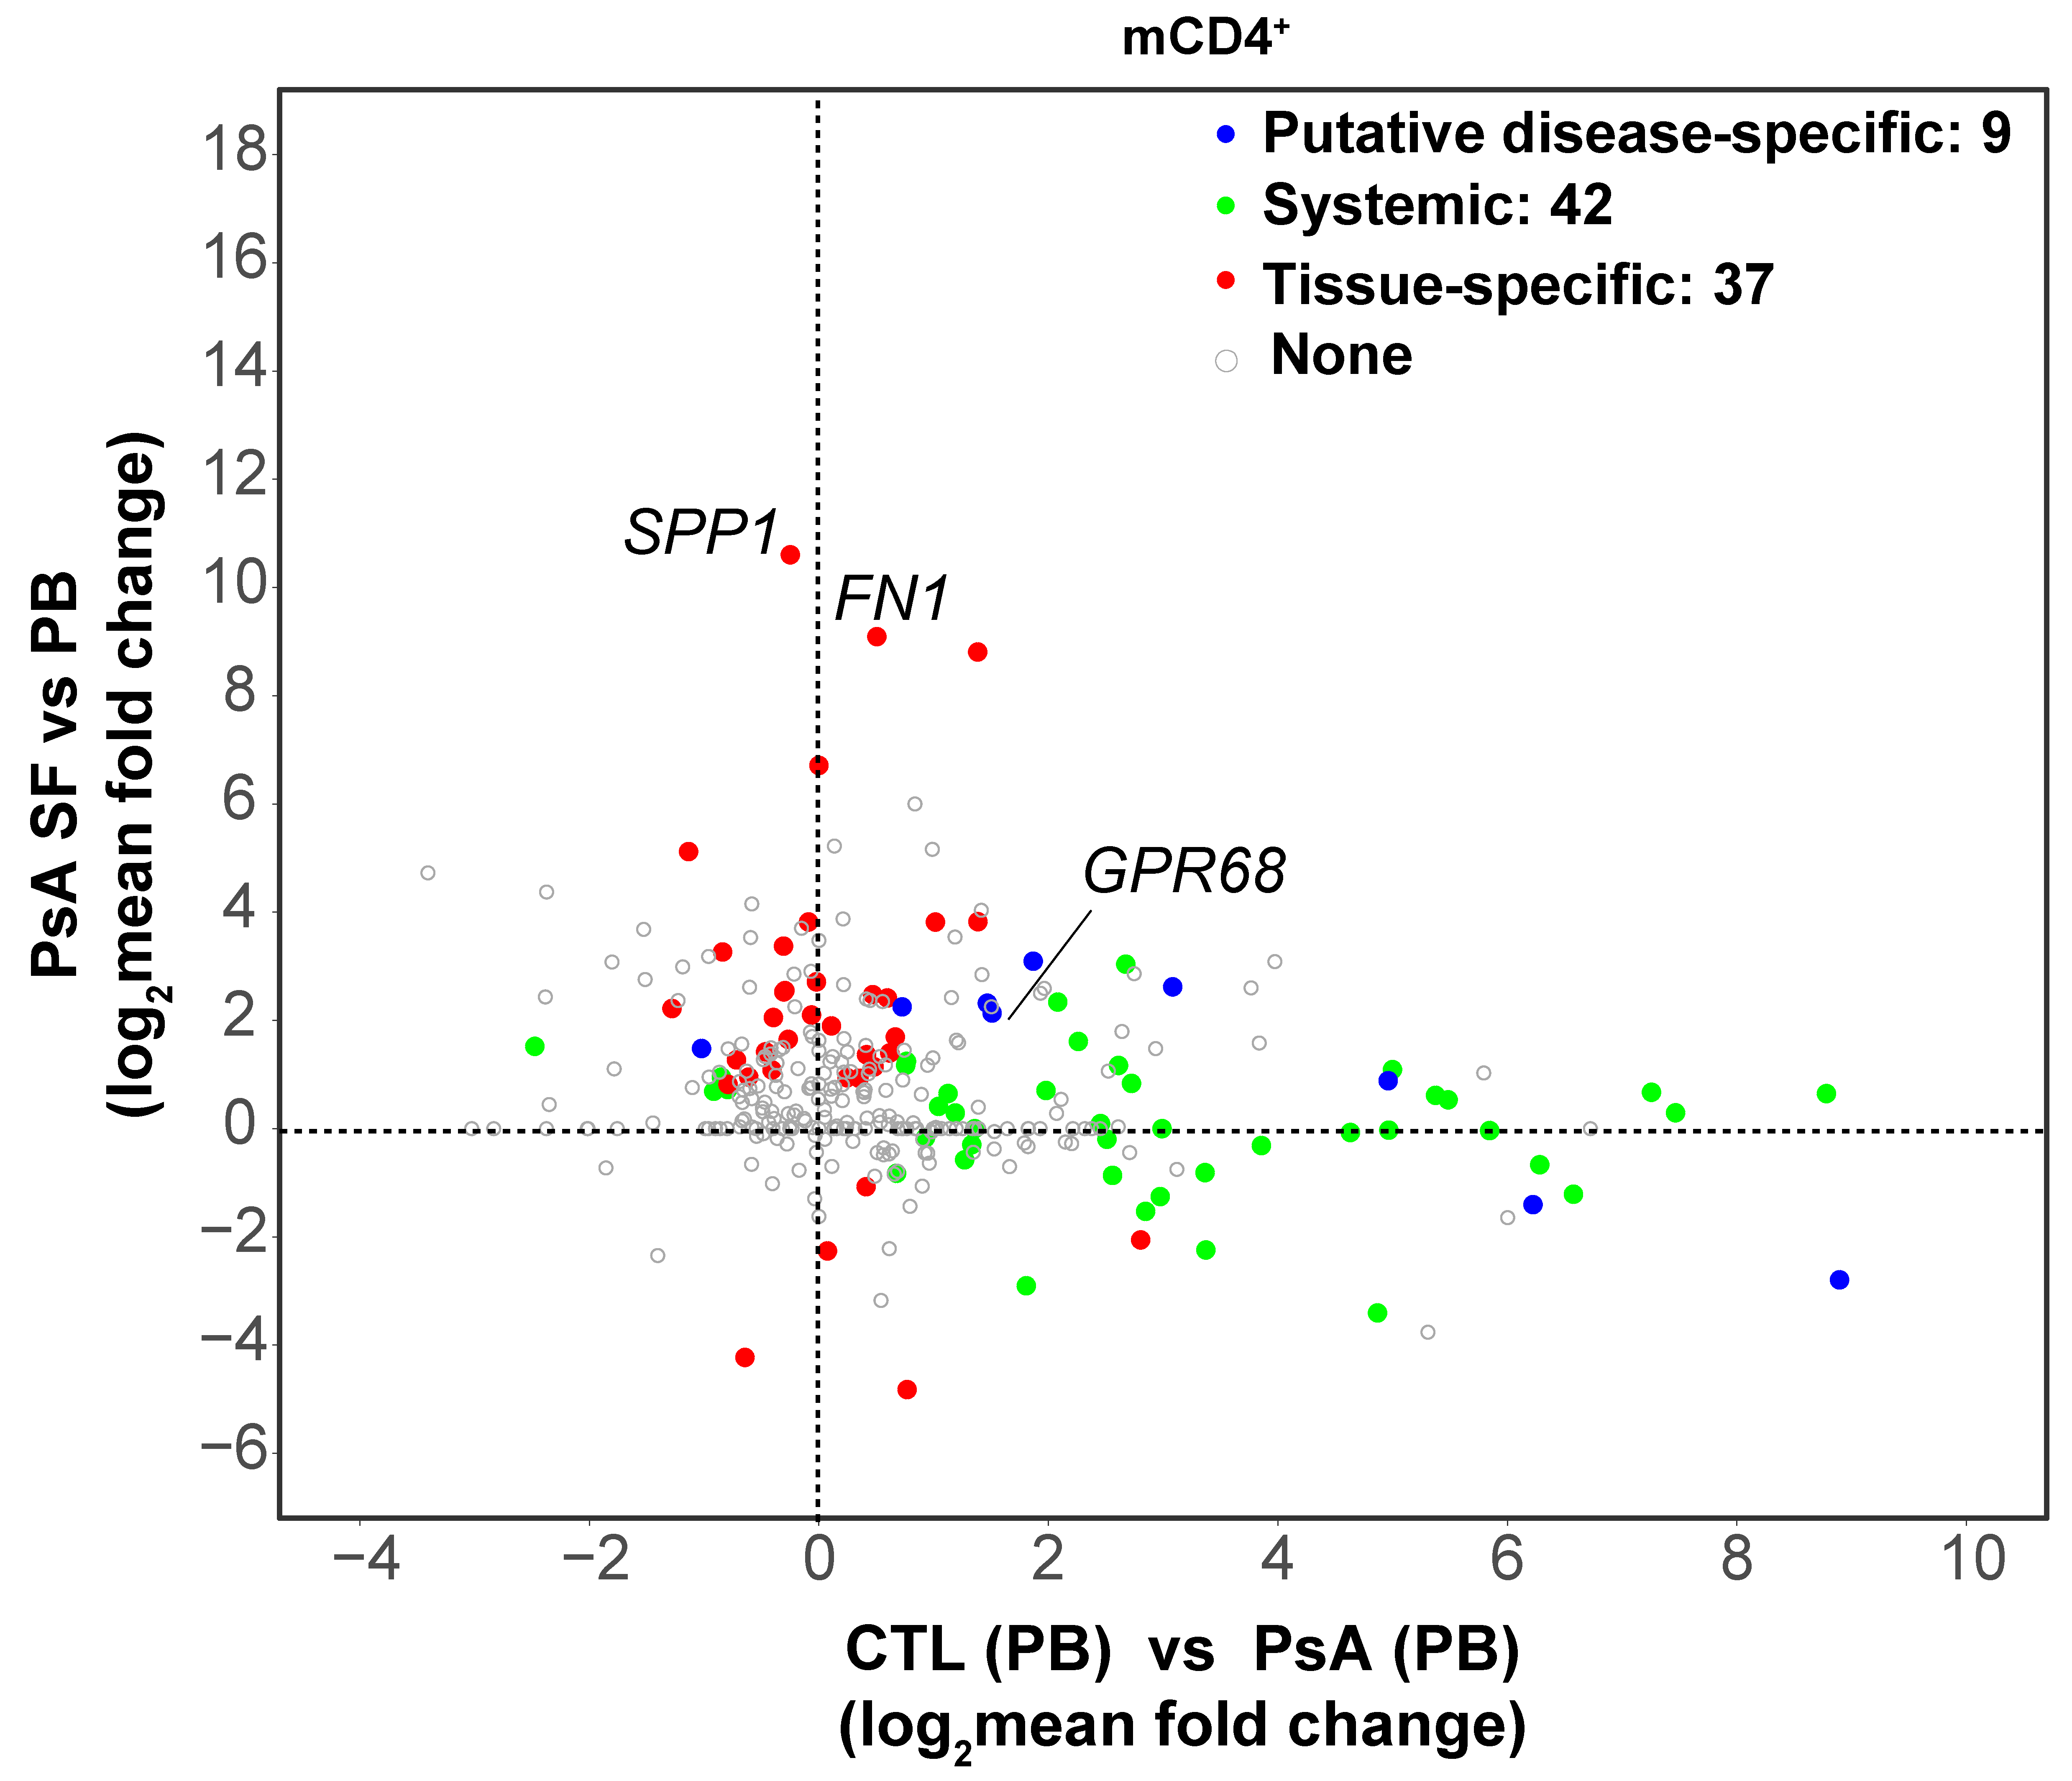
\includegraphics[width=\textwidth]{./Results3/pdfs/PSA_array_correlation_CD4_FC_HVPsA_vs_SFPBPsA}
%\caption{\textbf{}}
%\end{subfigure} %
%\begin{subfigure}{0.45\textwidth}
%\centering
%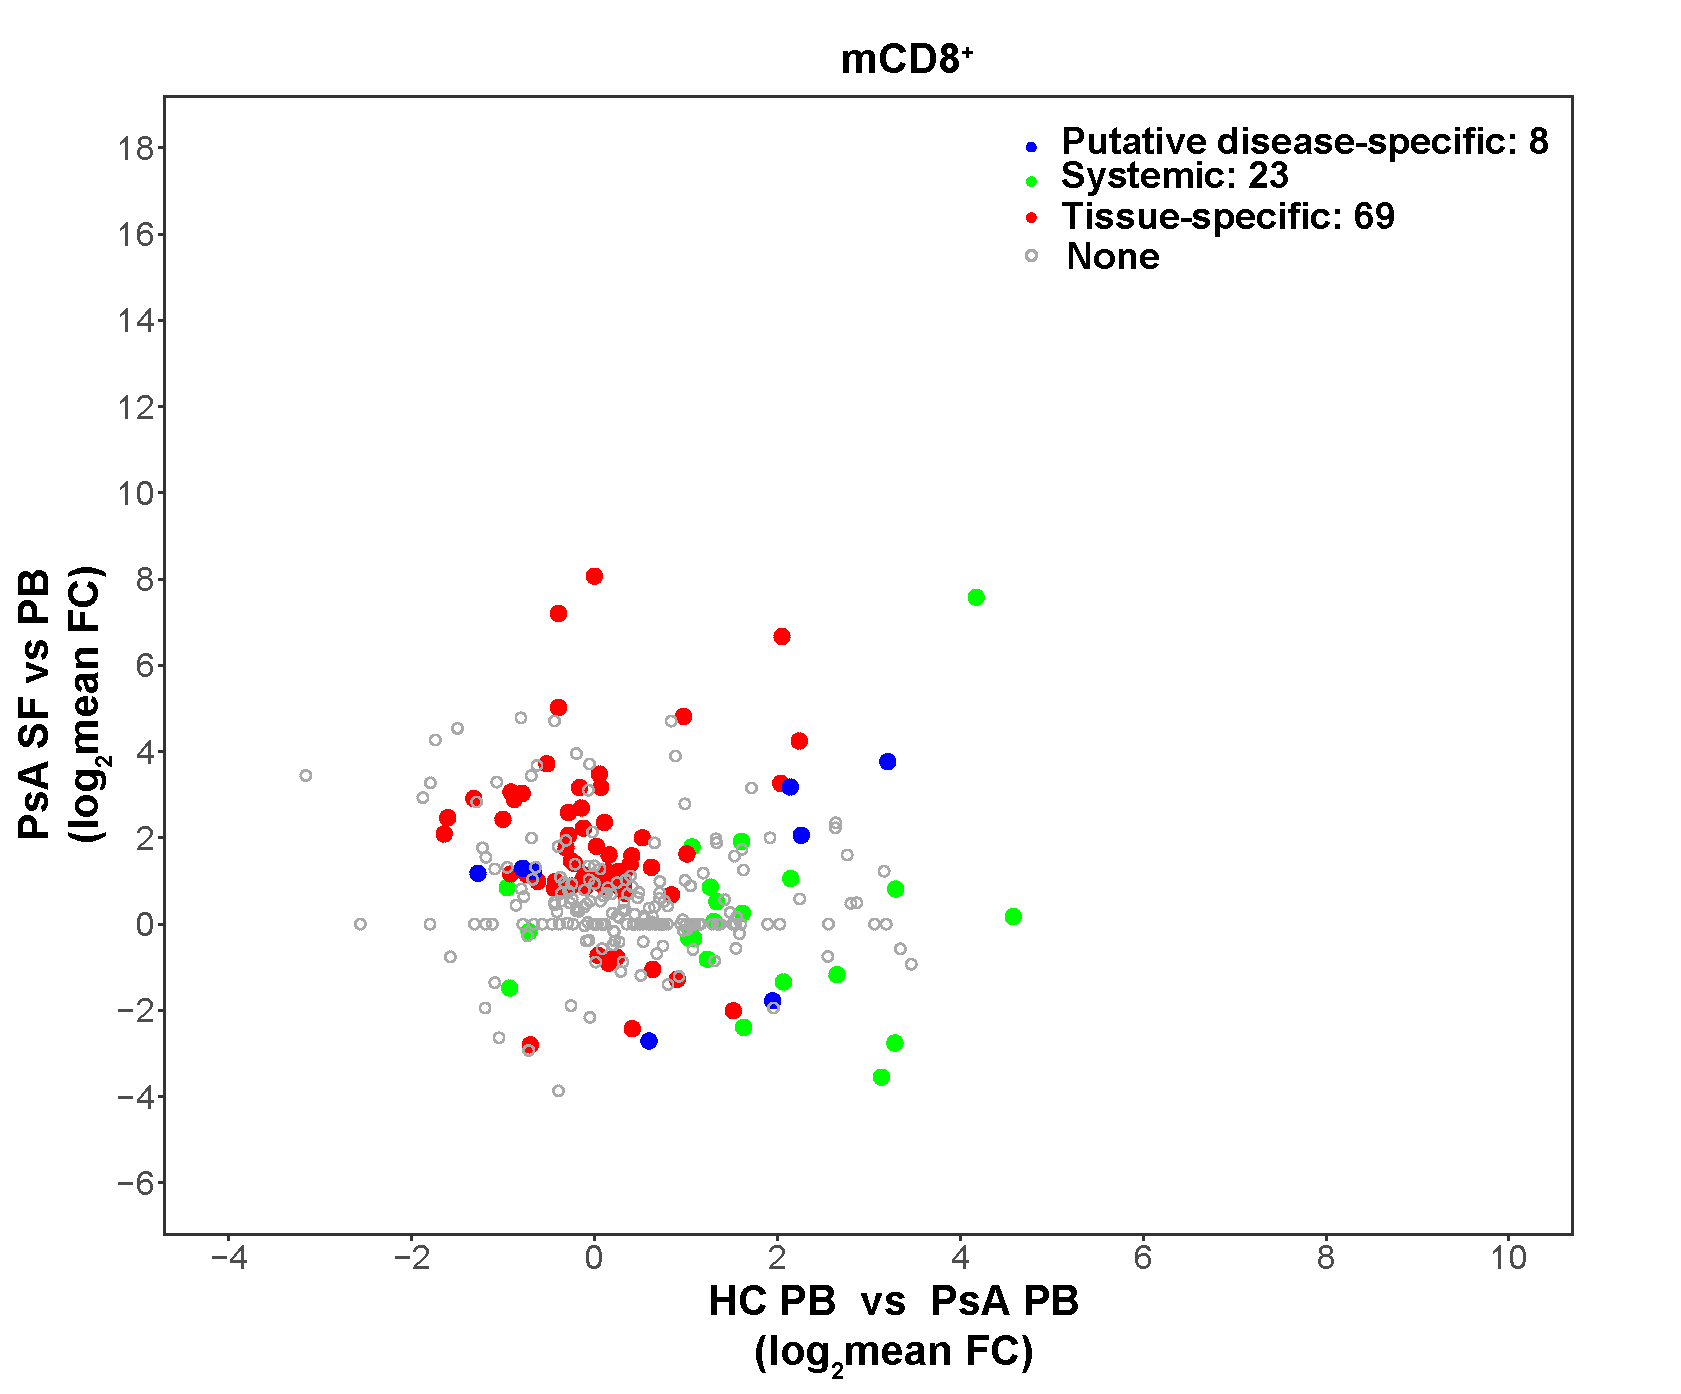
\includegraphics[width=\textwidth]{./Results3/pdfs/PSA_array_correlation_CD8_FC_HVPsA_vs_SFPBPsA}
%\caption{\textbf{}}
%\end{subfigure}
%\caption[Comparison of immune-relevant gene expression modulation across PsA tissues (synovial fluid vs PB) and in PsA patients verus healthy controls.]{\textbf{Comparison of immune-relevant gene expression modulation across PsA tissues (synovial fluid vs PB) and in PsA patients verus healthy controls.} The qPCR log${_2}$ mean fold change for each of the genes in the PsA synovial fluid vs peripheral blood contrast are plotted against the log${_2}$ mean fold change for the same genes in the PsA peripheral blood vs healthy control peripheral blood contrast in (A)CD14$^+$ monocytes, (B)mCD4$^+$ and (C) mCD8$^+$ cells. The genes are colour-coded based three categories of genes built according by comparison of changes in gene modulation between the two contrasts: only significantly modulated in peripheral blood between controls and PsA (systemic genes), only significantly modulated between synovial fluid and peripheral blood in PsA patients (tissue-specific) and significantly modulated between controls and PsA patients in peripheral blood as well as between synovial fluid and peripheral blood in PsA patients (putative disease-specific).}
%\label{figure:PSA_PCR_array_HC_FC_correlation}
%\end{figure} 


%
%A second group of genes were designated as tissue-specific, since they were significantly modulated between synovial fluid and peripheral blood in PsA patients but did not show significant changes between controls and PsA at the circulating level (Figure \ref{figure:PSA_PCR_array_HC_FC_correlation} red dots). Interestingly, in CD14$^+$ monocytes the tissue specific modulated genes considerably outnumbered the systemic ones (62 versus 14), showing a more pronounced change in the expression profile of immune genes across patients' tissues than between healthy and diseased peripheral blood (Figure \ref{figure:PSA_PCR_array_HC_FC_correlation} a red dots). For example, the aforementioned \textit{NFKB} and \textit{MYD88}, \textit{TLR2} genes were only up-regulated in PsA synovial fluid CD14$^+$ monocytes and their expression was not significantly modulated between healthy controls and PsA circulating CD14$^+$ monocytes.  Similarly to CD14$^+$ monocytes, mCD8$^+$ cells also presented greater disease tissue-specific modulation than genes differentially expressed when compared to controls in peripheral blood (Figure \ref{figure:PSA_PCR_array_HC_FC_correlation} c red dots). For all three cell types, the two genes presenting the greatest fold change between synovial fluid and peripheral blood \textit{SPP1} and \textit{FN1} appeared to be tissue-specific genes and no significant changes in peripheral blood between PsA and healthy controls were identified.
%%Some more biology?
%% talk about limitations in acknowledging these genes as dissease-tissue specific due to the fact that we don't know if they also change between peripheral blood and Sf in HV
%
%The third category comprised genes significantly modulated for each cell type between controls and PsA patients in peripheral blood as well as between synovial fluid and peripheral blood in PsA patients. These genes defined as putative disease-specific genes presented similar numbers across CD14$^+$ monocytes, mCD4$^+$ and mCD8$^+$ (10, 9 and 8, respectively) (Figure \ref{figure:PSA_PCR_array_HC_FC_correlation} blue dots in a, b and c). In CD14$^+$ monocytes two of those genes, \textit{GPI} and \textit{PRG2}, were up-regulated in both comparisons, with further exacerbation in synovial fluid (Figure \ref{figure:PSA_PCR_array_HC_FC_correlation} a). Evidence of the glucose-6-phosphate isomerase \textit{GPI} up-regulation in disease has been found in RA synovial fibroblasts and linked to increased levels of TNF-$\alpha$ and IL-1$\beta$ in the synovium \parencite{Zhong2015}. % GPI fibroblasts https://www.ncbi.nlm.nih.gov/pmc/articles/PMC4422595/
%Another example of exacerbated up-regulation in synovial fluid was the expression of \textit{GPR68} in mCD4$^+$. This gene was up-regulated in PsA peripheral blood mCD4$^+$ when compared to the control counterparts and further up-regulated in synovial fluid when compared to peripheral blood in PsA individuals (Figure \ref{figure:PSA_PCR_array_HC_FC_correlation} b). %\textit{GPR68} is a G protein-coupled receptor, expressed in T cells, amongst other cells, that undergoes activation through pH acidification, characteristic of synovial tissues under inflammation \parencite{Biniecka2016}. \textit{GPR68} activation leads to an increase of Ca$^2$$^+$ levels and subsequent activation of immune-related pathways \parencite{Saxena2011}. 
%\textit{GPR68} was also up-regulated in synovial fluid compared to peripheral blood in mCD8$^+$ cells, reinforcing the relevance of this gene in the synovial pathophysiological aspect of PsA. Amongst the genes presenting an opposite behavior is the epidermal growth factor-like amphiregulin (\textit{AREG}), which in mCD8$^+$ is significantly up-regulated in PsA peripheral blood compared to the controls but is down-regulated in PsA individuals when comparing synovial fluid versus peripheral blood (Figure \ref{figure:PSA_PCR_array_HC_FC_correlation} c). %\textit{AREG} deficiency in mouse models have shown an impaired immunosupressive response by Treg cells \parencite{Zaiss2013}, which could be contributing to the exacerbated immune response in the synovium. 
%% GPR68 https://ard.bmj.com/content/73/Suppl_2/511.2
%%GPR68 Hypoxia Positively Regulates the Expression of pH-Sensing G-Protein–Coupled Receptor OGR1 (GPR68)
%%talk about limitations of those genes to be identified as disease specific. This would need an additional comparison between HV synovial fluid and PsA synovial fluid to make sure that those genes are not modulated in synovial fluid of HV and therefore are a lanmark of disease in both tissues
%Despite the interesting aforementioned findings, the identification of disease-specific and disease tissue-specific genes is clearly limited by the impossibility of obtaining healthy controls synovial fluid to include in the experimental design. 
%
%When performing pathway enrichment analysis using the significantly modulated genes between healthy controls and PsA patients peripheral blood in the qPCR array, only the Reactome immune system pathway appeared as significant for CD14$^+$ monocytes and mCD4$^+$ cells. This result reinforced the tissue-specificity of the pathways enriched for the modulated genes between synovial fluid and peripheral blood in CD14$^+$ monocytes PsA patients and clearly suggest a more pronounced inflammatory phenotype of the pathological CD14$^+$ monocytes in synovial fluid compared to PB.



\subsection{Characterisation of CD14$^+$ monocyte heterogeneity in PsA using scRNA-seq}
According to the analysis of chromatin accessibility and immune-related gene expression in this pilot cohort, CD14$^+$ monocytes showed the largest number of significant DARs and the most reliable modulation of expression, highlighting changes in expression between peripheral blood and synovial fluid for pro-inflammatory chemokines and cytokines. Monocytes are very plastic cells which initiate differentiation into macrophages at the site of inflammation. Therefore, exploring differences at the single-cell level may identify subpopulations with particular phenotypes of interest and may also highlight differences in the immune response driven by this cell type in circulation and at the inflamed synovium.


\subsubsection{Exploration of monocyte subsets in synovial fluid and peripheral blood}
%Explain how I did the analysis
First, scRNA-seq analysis was performed in paired PBMCs and SFMCs isolated from three PsA patients (Table \ref{tab:PSA_datasets_per_sample}). scRNA-seq data from each of the PBMCs and SFMCs samples were downsampled to 3,000 cells and filtered to remove genes that were expressed only in few cells and those cells expressing low number of genes (as described in Chapter \ref{ch:Mat}). The monocyte population sorted by FACS was characterised for expressing the surface marker CD14$^+$. For consistency, the scRNA-seq monocyte population for downstream analysis was identified based on expression of \textit{CD14} and \textit{LYZ}, two canonical markers of CD14$^+$ monocytes \parencite{Zhao2009}(Figures \ref{figure:PsA_scRNAseq_SF_an_PB_monocytes_markers_and_tissue_identity}A and B and \ref{figure:PsA_scRNAseq_SF_an_PB_monocytes_identification_from_bulk}A and B). After additional filtering to remove cells with abundant mitochondrial reads and excessive number of unique molecular identifiers (UMI) a total of 2,798 cells across the six samples were identified as CD14$^+$ monocytes (1,537 and 1,261 from synovial fluid and peripheral blood, respectively). This represented approximately 15\% of the bulk SFMCs and PBMCs cells included in the analysis and in line with the proportion of CD14$^+$ monocytes previously reported using cell surface markers by mass cytometry (Figure \ref{figure:PsA_cell_composition}). Interestingly, expression of the low-affinity immunoglobulin G Fc$\gamma$ receptor (Fc$\gamma$RIIa) CD16$^+$ by the synovial fluid CD14$^+$ monocytes suggested a more intermediate phenotype (CD14$^+$+ CD16$^+$) in this tissue compared to peripheral blood monocytes showing a more classical phenotype (CD14$^+$ CD16$^-$) (Figure \ref{figure:PsA_scRNAseq_SF_an_PB_monocytes_markers_and_tissue_identity}C). Subsequent visualisation using uniform manifold approximation and projection (UMAP) clearly separated the synovial fluid and peripheral blood CD14$^+$ monocyte populations (Figure \ref{figure:PsA_scRNAseq_SF_an_PB_monocytes_markers_and_tissue_identity}D). 


\bigskip
\begin{figure}[H]
\centering
\begin{subfigure}[b]{0.40\textwidth}
\centering 
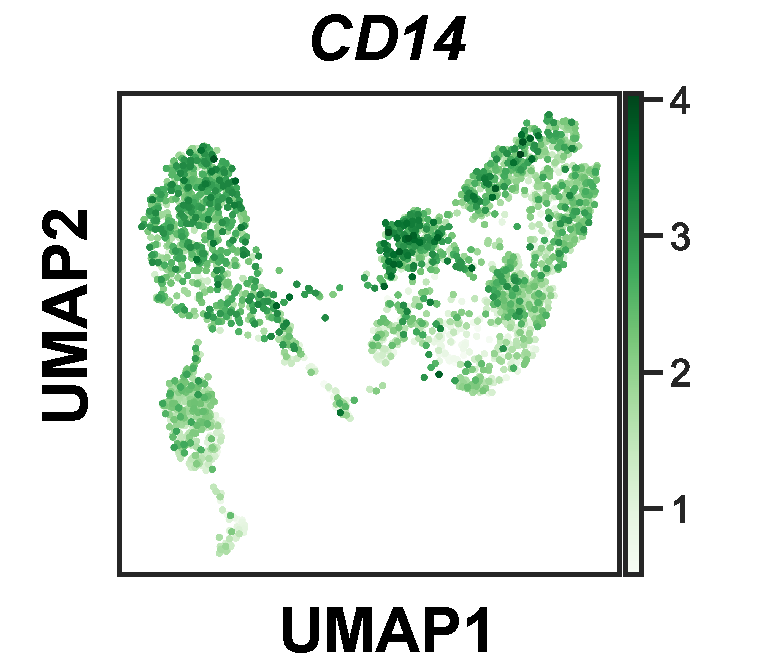
\includegraphics[width=\textwidth]{./Results3/pdfs/PSA_monocytes_scanpy_single_cell_CD14_UMAP}
\caption{}
\end{subfigure}
~
\begin{subfigure}[b]{0.40\textwidth} 
%the [b] prevents offset in subcaptions
\centering
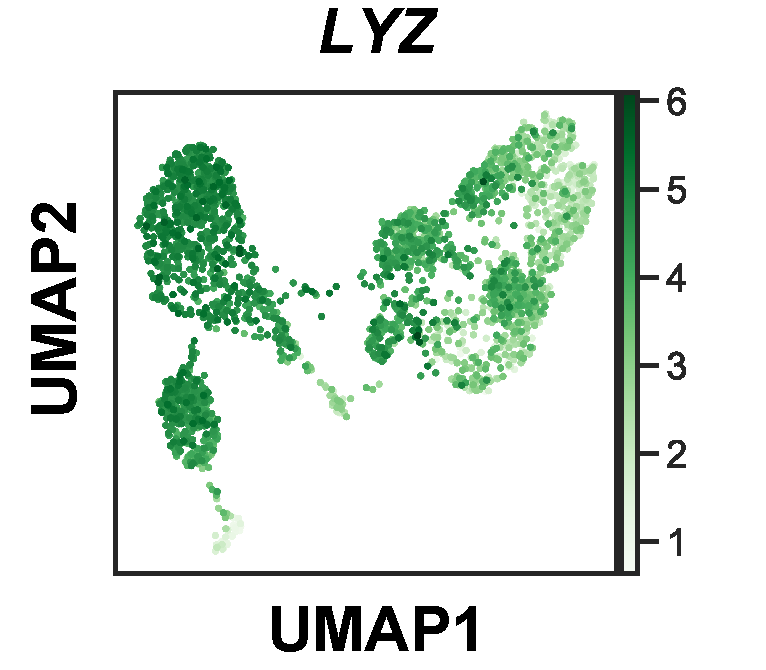
\includegraphics[width=\textwidth]{./Results3/pdfs/PSA_monocytes_scanpy_single_cell_LYZ_UMAP}
\caption{}
\end{subfigure}
~
\begin{subfigure}[b]{0.40\textwidth} 
	%the [b] prevents offset in subcaptions
	\centering
	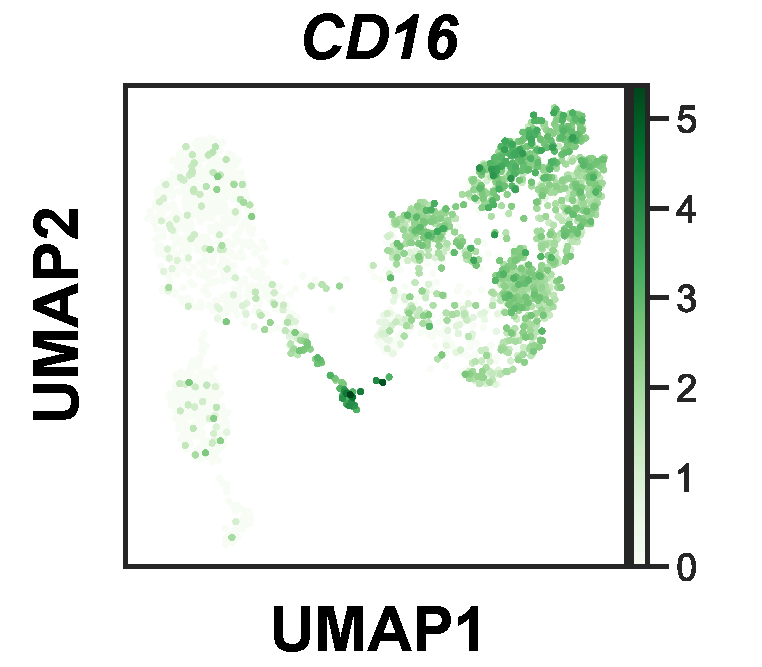
\includegraphics[width=\textwidth]{./Results3/pdfs/PSA_monocytes_scanpy_single_cell_CD16_UMAP}
	\caption{}
\end{subfigure}%
~
\begin{subfigure}[b]{0.45\textwidth} 
%the [b] prevents offset in subcaptions
\centering
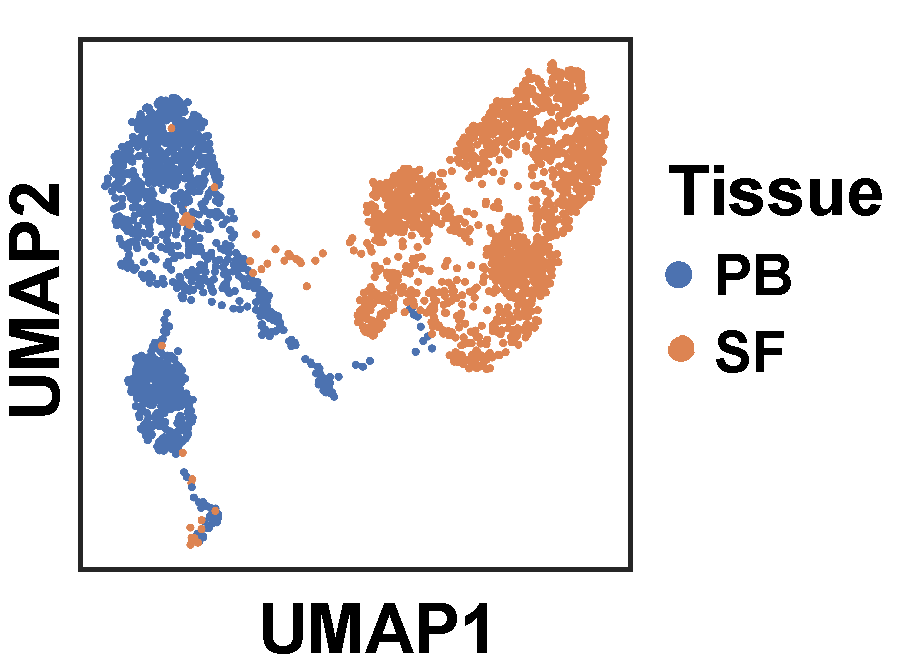
\includegraphics[width=\textwidth]{./Results3/pdfs/PSA_monocytes_scanpy_single_cell_SF_PB_UMAP}
\caption{}
\end{subfigure}
\caption[Visualisation using UMAP dimensional reduction of the synovial fluid and peripheral blood CD14$^+$ monocytes.]{\textbf{Visualisation using UMAP dimensional reduction of the synovial fluid and peripheral blood CD14$^+$ monocytes.} Visualisation using UMAP dimensional reduction of (A) \textit{CD14}, (B) \textit{LYZ} and \textit{CD16} expression intensities in the combined synovial fluid and peripheral blood CD14$^+$ monocytes cells. (C) Overlaid colour-coded tissue identity for each of the CD14$^+$ monocytes cells from the combined population (orange or blue for synovial fluid and peripheral blood, respectively).}
\label{figure:PsA_scRNAseq_SF_an_PB_monocytes_markers_and_tissue_identity}
\end{figure}

Cluster analysis was conducted in the combined population of synovial fluid and peripheral blood CD14$^+$ monocytes using standard default resolution of the Leiden clustering algorithm (detailed in Chapter \ref{ch:Mat}). Using these parameters, 8 CD14$^+$ monocyte clusters (MC) were identified, with MC-1 to MC-4 predominantly formed by synovial fluid monocytes and clusters MC-5,6 and 8  being mostly of peripheral blood origin (Figure \ref{figure:PsA_scRNAseq_SF_an_PB_monocytes_clusters_and_vln_plots}A). MC-1 and MC-6 were the largest synovial fluid and peripheral blood clusters, respectively, representing 40.7 and 65.8\% of the total number of monocytes of each tissue (Figure \ref{figure:PsA_scRNAseq_SF_an_PB_monocytes_clusters_and_vln_plots}A). 

\begin{figure}[H]
	\centering
	\begin{subfigure}[b]{0.65\textwidth}
		\centering 
		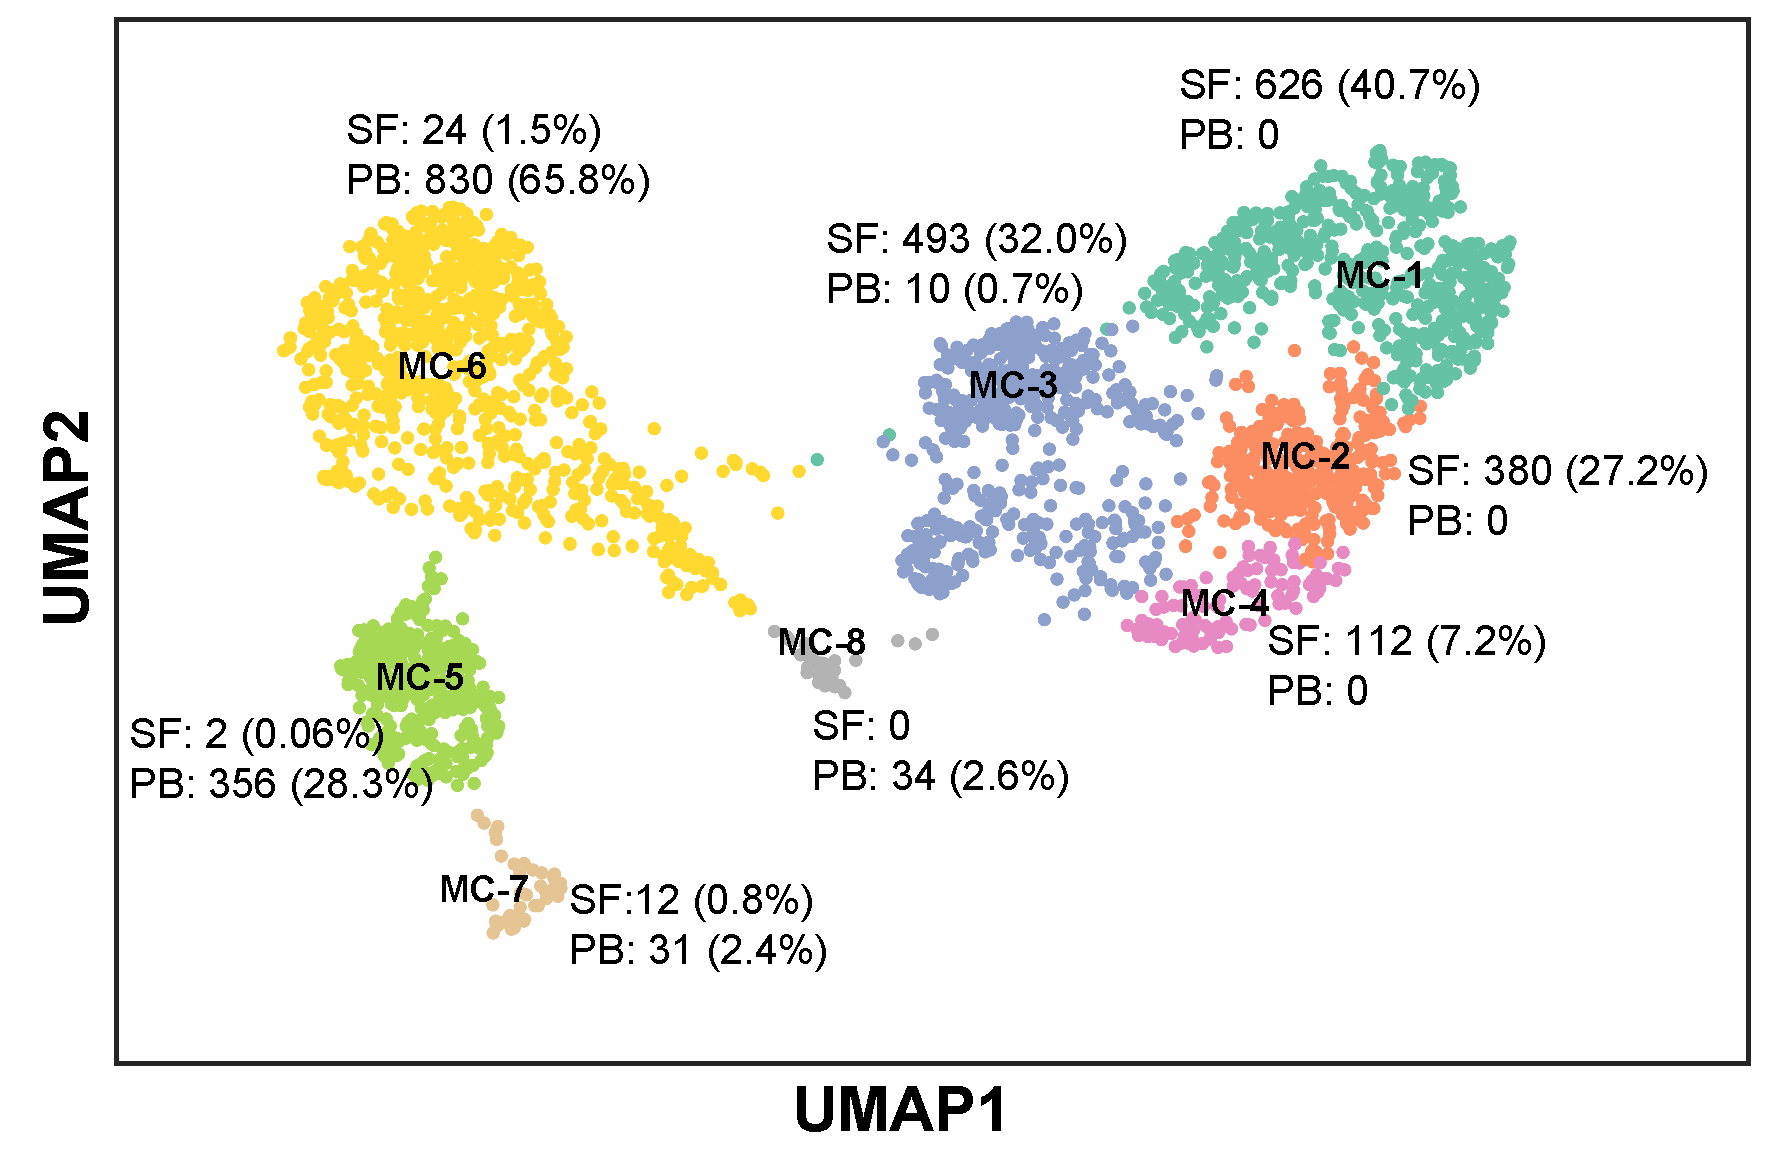
\includegraphics[width=\textwidth]{./Results3/pdfs/PSA_monocytes_scanpy_single_cell_cluster_UMAP}
		\caption{}
	\end{subfigure}
	~
	\begin{subfigure}[b]{0.35\textwidth} 
		%the [b] prevents offset in subcaptions
		\centering
		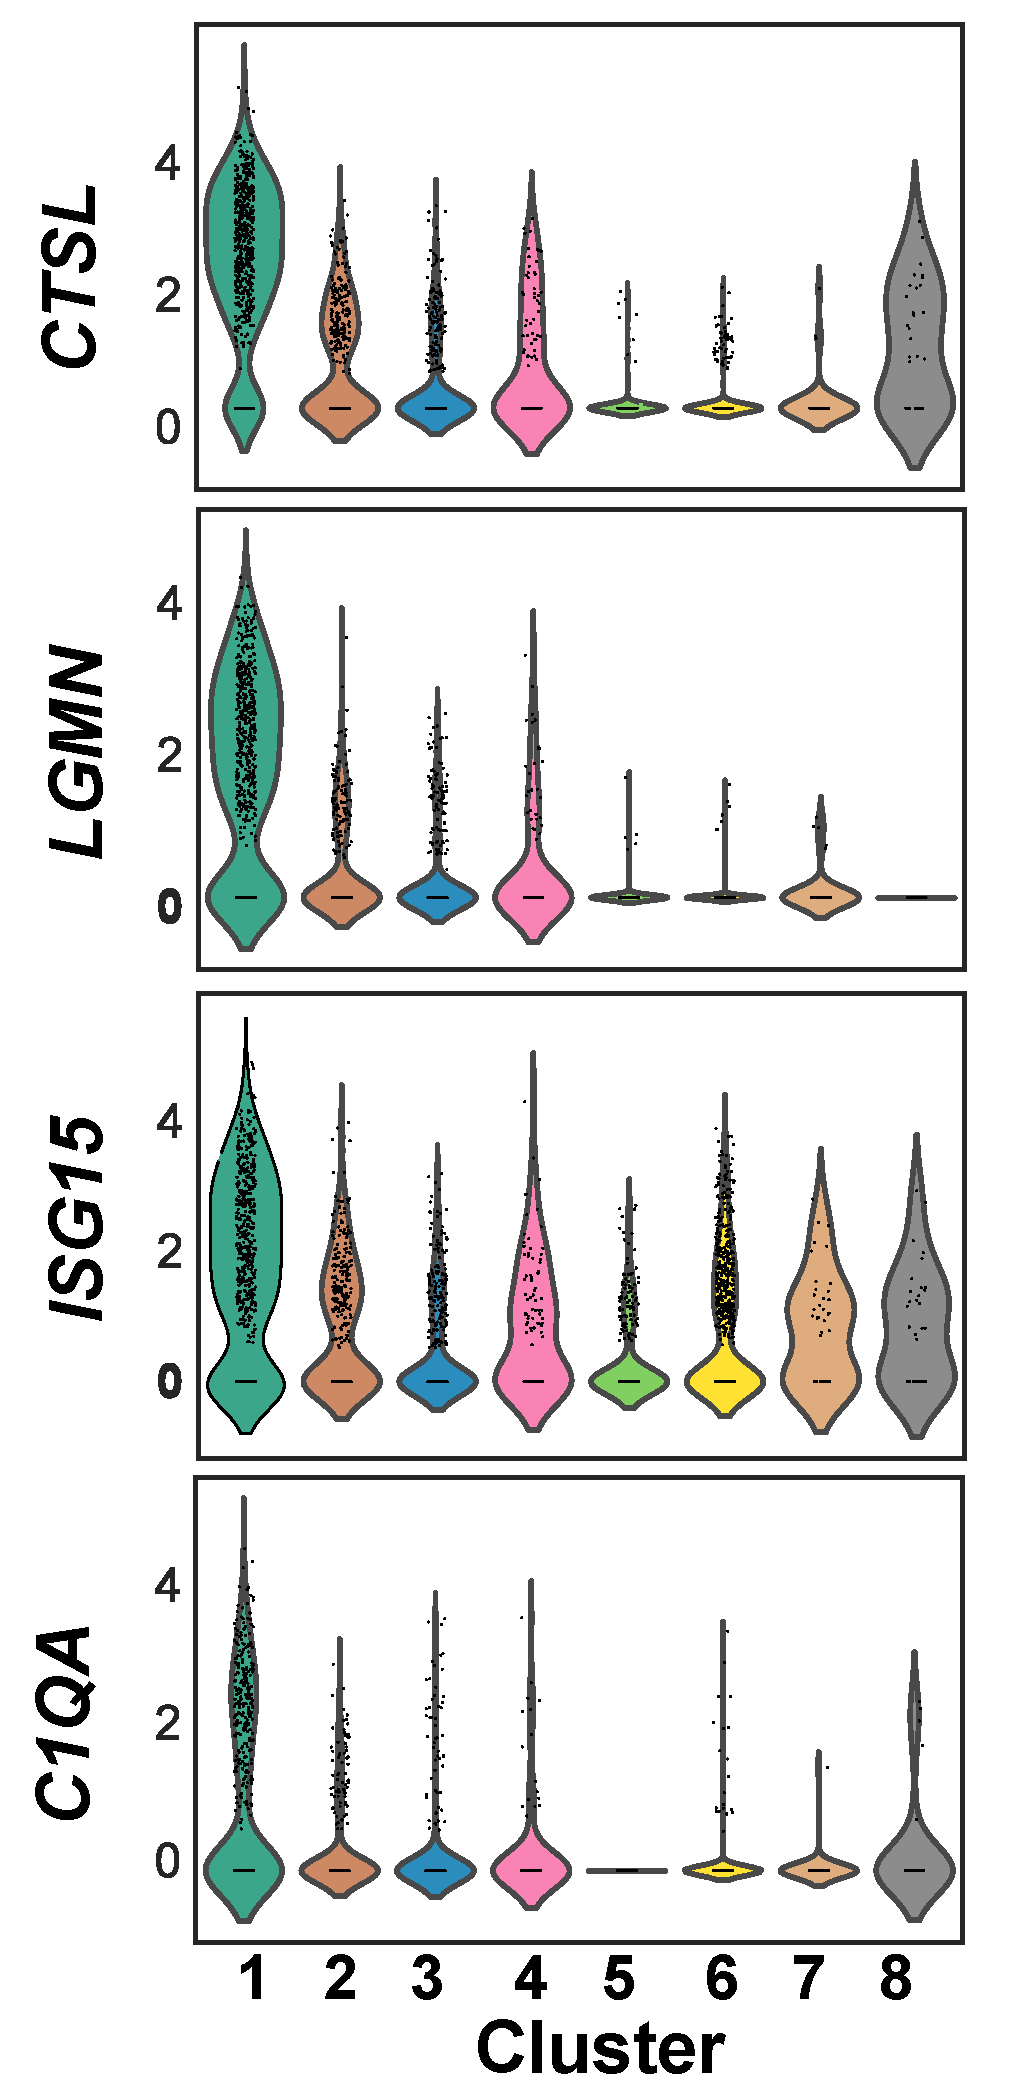
\includegraphics[width=\textwidth]{./Results3/pdfs/PSA_monocytes_scanpy_single_cell_vln_plots_C1}
		\caption{}
	\end{subfigure}%
	~
	\begin{subfigure}[b]{0.35\textwidth} 
		%the [b] prevents offset in subcaptions
		\centering
		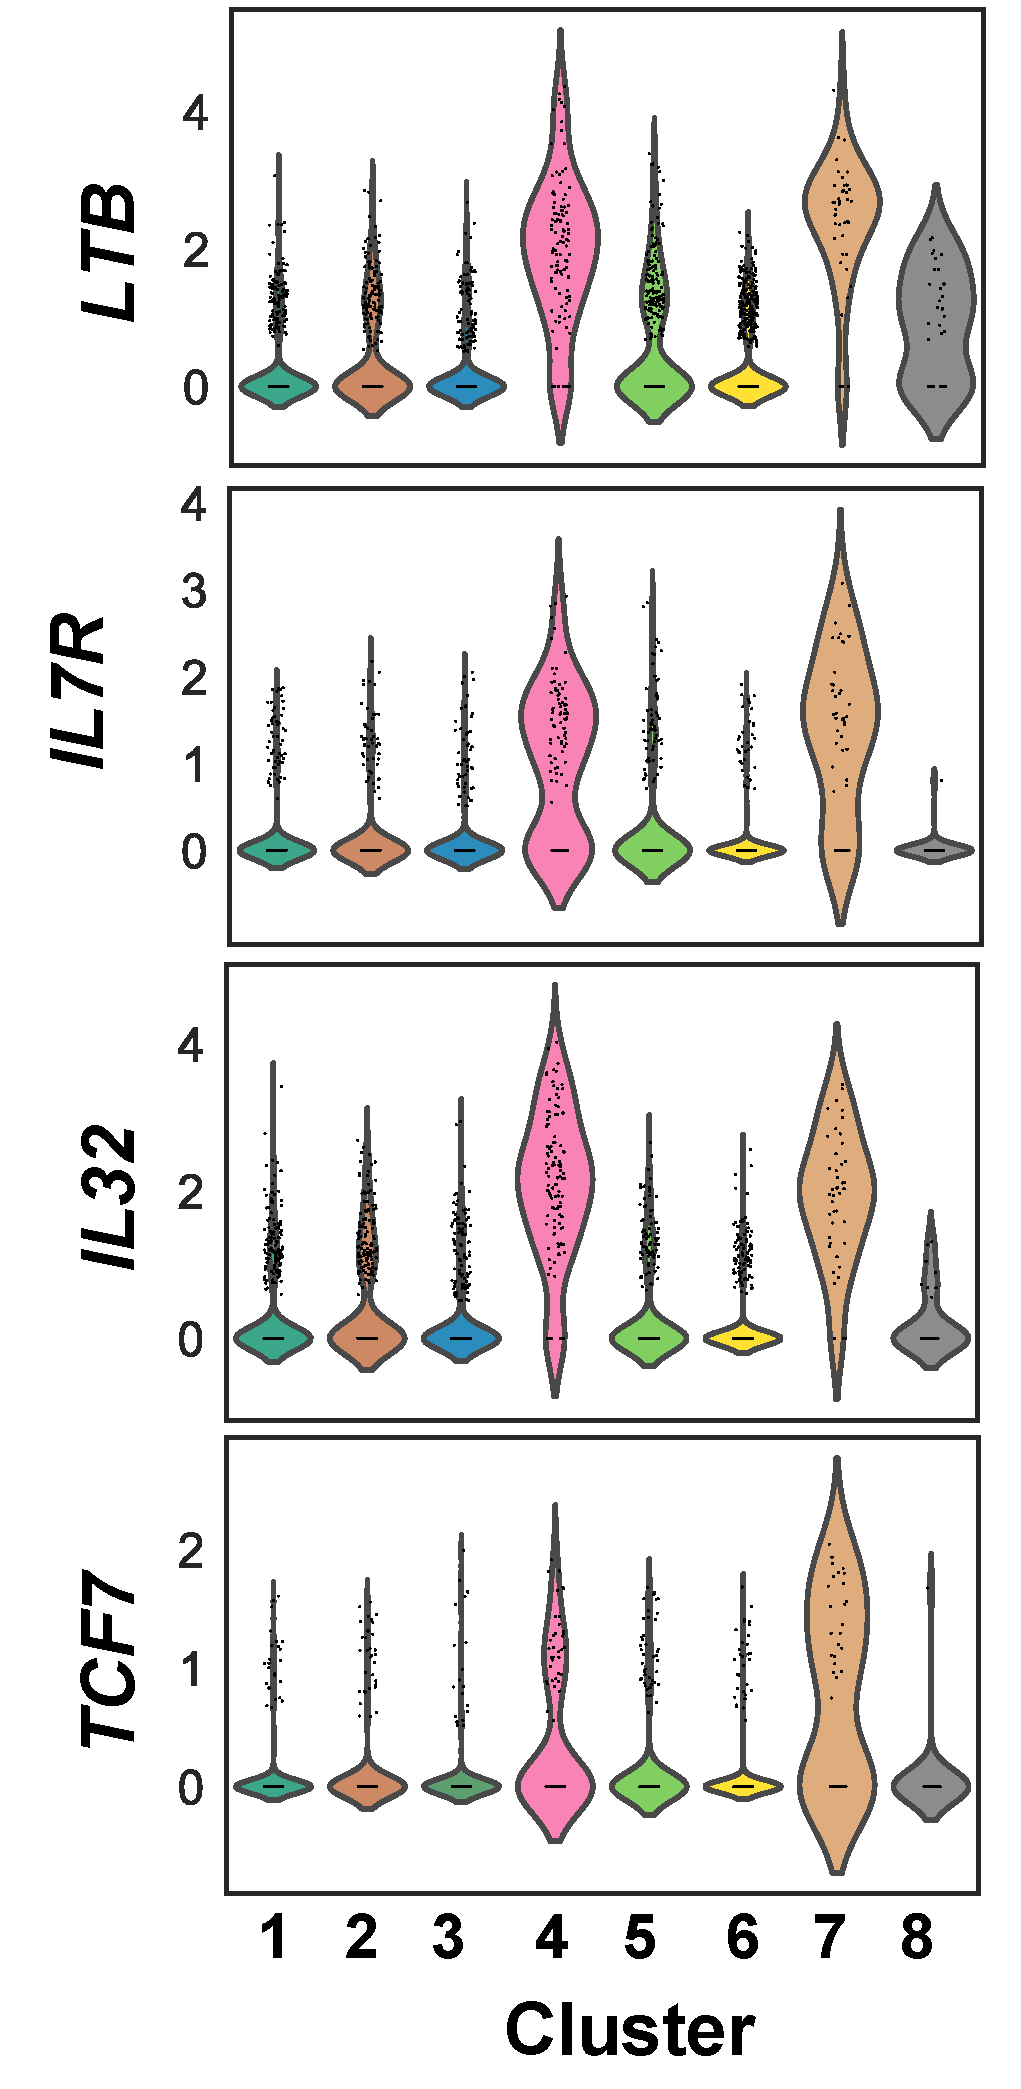
\includegraphics[width=\textwidth]{./Results3/pdfs/PSA_monocytes_scanpy_single_cell_vln_plots_C4}
		\caption{}
	\end{subfigure}
	\caption[Identification and characterisation of CD14$^+$ monocytes subpopulations in synovial fluid and peripheral blood.]{\textbf{Identification and characterisation of CD14$^+$ monocytes subpopulations in synovial fluid and peripheral blood.} (A) Visualisation using UMAP dimensional reduction of the CD14$^+$ monocytes subpopulations identified in the combined synovial flui and peripheral blood CD14$^+$ monocytes. For each cluster the number of cells and the  percentage over the total number of cells from the corresponding tissue are indicated. Violin plots representing for MC-1 to MC-8 (x-axis) the probability density of expression (y-axis) for marker genes charcateristic of the (B) MC-1 and (C) MC-4 subpopulations. SF=synovial fluid; PB=peripheral blood.}
\label{figure:PsA_scRNAseq_SF_an_PB_monocytes_clusters_and_vln_plots}
\end{figure}

MC-7 was the cluster with the most even contribution of CD14$^+$ monocytes from the two tissues (0.8 and 2.4\% from synovial fluid and peripheral blood, respectively). MC-7 may be a real cluster or result from remaining unfiltered layouts or cell miss classification by the clustering algorithm and additional sample size will be required to confirm this cluster identity. Each of the 8 CD14$^+$ monocytes clusters was characterised by a number of marker genes, a set of significant up-regulated genes by the cells of that particular subpopulation when compared to the rest of the cells (Figure \ref{figure:PSA_scRNAseq_SF_PB_heatmap_8_top_markers}). The heatmap illustrating expression levels of the top marker genes in each of the clusters only showed moderate differences across the subpopulations formed by monocytes of the same tissue but displayed a very distinct pattern of expression across tissues (Figure \ref{figure:PSA_scRNAseq_SF_PB_heatmap_8_top_markers}). 


\begin{figure}[htbp]
\centering
\includegraphics[width=\textwidth]{./Results3/pdfs/PSA_monocytes_scanpy_single_cell_monocytes_clusters_heatmap}
\caption[Heatmap and hierarchical clustering for the top eight marker genes of the CD14$^+$ monocyte subpopulations identified in synovial fluid and peripheral blood from three PsA patients.]{\textbf{Heatmap and hierarchical clustering for the top eight marker genes of the CD14$^+$ monocyte subpopulations identified in synovial fluid and peripheral blood from three PsA patients.} The rows represent the genes and the columns correspond to each of the cells analysed in the experiment. The heatmap illustrates the relative expression (log$_2$fold change in a particular cell of the cluster compared to the average expression of all the cells from the other clusters) for the top eight marker genes defining each of the eight clusters. Dendogram indicating hierarchical relationship between clusters is indicated at the top and cluster identity for each of the cells is specified at the bottom.}
\label{figure:PSA_scRNAseq_SF_PB_heatmap_8_top_markers}
\end{figure}


\subsubsection{Functional exploration of synovial fluid and peripheral blood CD14$^+$ monocytes subpopulations}

Amongst the synovial fluid clusters, MC-1 and MC-4 appeared to be of particular interest based on their distinctive marker genes. MC-1 presented significant up-regulated expression of IFN-related genes  such as \textit{CTSL}, \textit{ISG15}, \textit{IFI6} or \textit{IFI27}, genes involved in antigen presentation such as \textit{LGMN} and members of the complement cascade, especially the \textit{C1QA} when compared to all the other clusters. Gene ontology analysis using all the significant up-regulated genes (FDR$<$0.01 and fold change$>$1.5) unique for this cluster  demonstrated enrichment of type-I IFN and IFN-$\gamma$ mediated signalling, response to virus, chemokine-mediated signalling and complement cascade, GO terms that were not found to be enriched for any of the remaining 7 clusters (Figure \ref{figure:PsA_scRNAseq_MC1_MC2_characterisation}A).


%LGMN Ag presentation https://www.nature.com/articles/25379

MC-4 represented 7.2\% of synovial fluid CD14$^+$ monocytes and was characterised by high expression of \textit{IL7R}, the IL-7 regulated cytokines \textit{LTB}, the TF \textit{TCF7}, the pro-inflammatory cytokine induced of TNF-$\alpha$ \textit{IL-32}  \parencite{Kim2005} and the chemokine \textit{CCL5} (Figures \ref{figure:PsA_scRNAseq_SF_an_PB_monocytes_clusters_and_vln_plots}C and \ref{figure:PSA_scRNAseq_SF_PB_heatmap_8_top_markers}). These genes were also up-regulated by the CD14$^+$ monocyte subpopulation expressing IL7R$^+$ upon \textit{in vitro} LPS stimulation conducted by Al-Mossawi and colleagues (in revision, Al-mossawi \textit{et al.},2018). MC-4 cluster showed differential expression of 340 genes (228 and 112 up- and down-regulated, respectively) when compared to the rest of the monocytes from the other clusters. These included the immunoregulatory non-coding RNA \textit{MALAT1} and the stabiliser of the TCR \textit{TRAT1}, amongst others (Figure \ref{figure:PsA_scRNAseq_MC1_MC2_characterisation}B). The DEGs (FDR$<$0.01) identified for the MC-4 subpopulation showed enrichment for the IL-7 responsive genes identified in IL7R$^+$ CD14$^+$ monocytes upon LPS stimulation in the aforementioned study \parencite{Al-Mossawi2018} (overlap of 116 genes, p-value=1.9x10$^{-13}$, Fisher exact test). Moreover, this set of DEGs showed enrichment for similar GO terms, including ribosomal biogenesis and protein translation, as the ones revealed by the up-regulated IL-7 CD14$^+$ monocytes responsive genes from Al-Mossawi and colleagues (Figure \ref{figure:PsA_scRNAseq_MC1_MC2_characterisation}C).

Interestingly, the mixed synovial fluid and peripheral blood MC-7 subpopulation (12 and 32 synovial fluid and peripheral blood cells, respectively) also showed up-regulation for some of MC-4 marker genes (Figures \ref{figure:PSA_scRNAseq_SF_PB_heatmap_8_top_markers} and \ref{figure:PsA_scRNAseq_SF_an_PB_monocytes_clusters_and_vln_plots}B). MC-7 only represented 2.4\% of the peripheral blood CD14$^+$ monocytes, suggesting that the subpopulation of CD14$^+$ monocytes expressing \textit{IL7R} (amongst the other markers) may be predominant and distinctive of the PsA synovial CD14$^+$ monocytes. This is consistent with the synovial fluid open DARs found at the promoter and 3'UTR of the transcriptional up-regulation (Figures \ref{figure:PsA_FAST_ATAC_gene_boy_DOCS_CD14_NK}A and \ref{figure:PSA_PCR_array_vulcano_plots}A).


Synovial fluid CD14$^+$ monocytes, particularly the MC-1 and MC-3 subpopulations expressed significant higher levels of a number of MHC-II genes, including  \textit{HLA-DRB1}, \textit{HLA-DPB1} or \textit{HLA-DRB5}, involved in the monocytes antigen presentation and T cell activation, in line with the intermediate monocytes phenotype (Figures \ref{figure:PsA_scRNAseq_ag_presentation_phagocytosis}A and \ref{figure:PSA_scRNAseq_SF_PB_heatmap_8_top_markers}). Moreover, peripheral blood CD14$^+$ monocytes showed greater expression of some of the phagocytic marker such as \textit{CD93}, \textit{CD36} and \textit{CLEC4E}, mostly driven by the MC-5 and MC-6 subpopulations and in line with their closer classic phenotype compared to the synovial fluid counterparts (Figure \ref{figure:PsA_scRNAseq_ag_presentation_phagocytosis}B), as well as genes from the S100 family, including \textit{S100A8} or \textit{S100A12} (Figure \ref{figure:PSA_monocytes_scanpy_single_cell_volcano_and_qPCR_ATAC_correlation}A). Nevertheless, the unique marker genes specific for other subpopulations did not reveal unique relevant functional roles for these clusters probably due to only moderate differences in the transcriptional profiles of the clusters within each tissue and additional sample size may help to characterise these populations or find additional ones.


\begin{figure}[htbp]
	\centering
	\begin{subfigure}[b]{0.48\textwidth}
		\centering 
		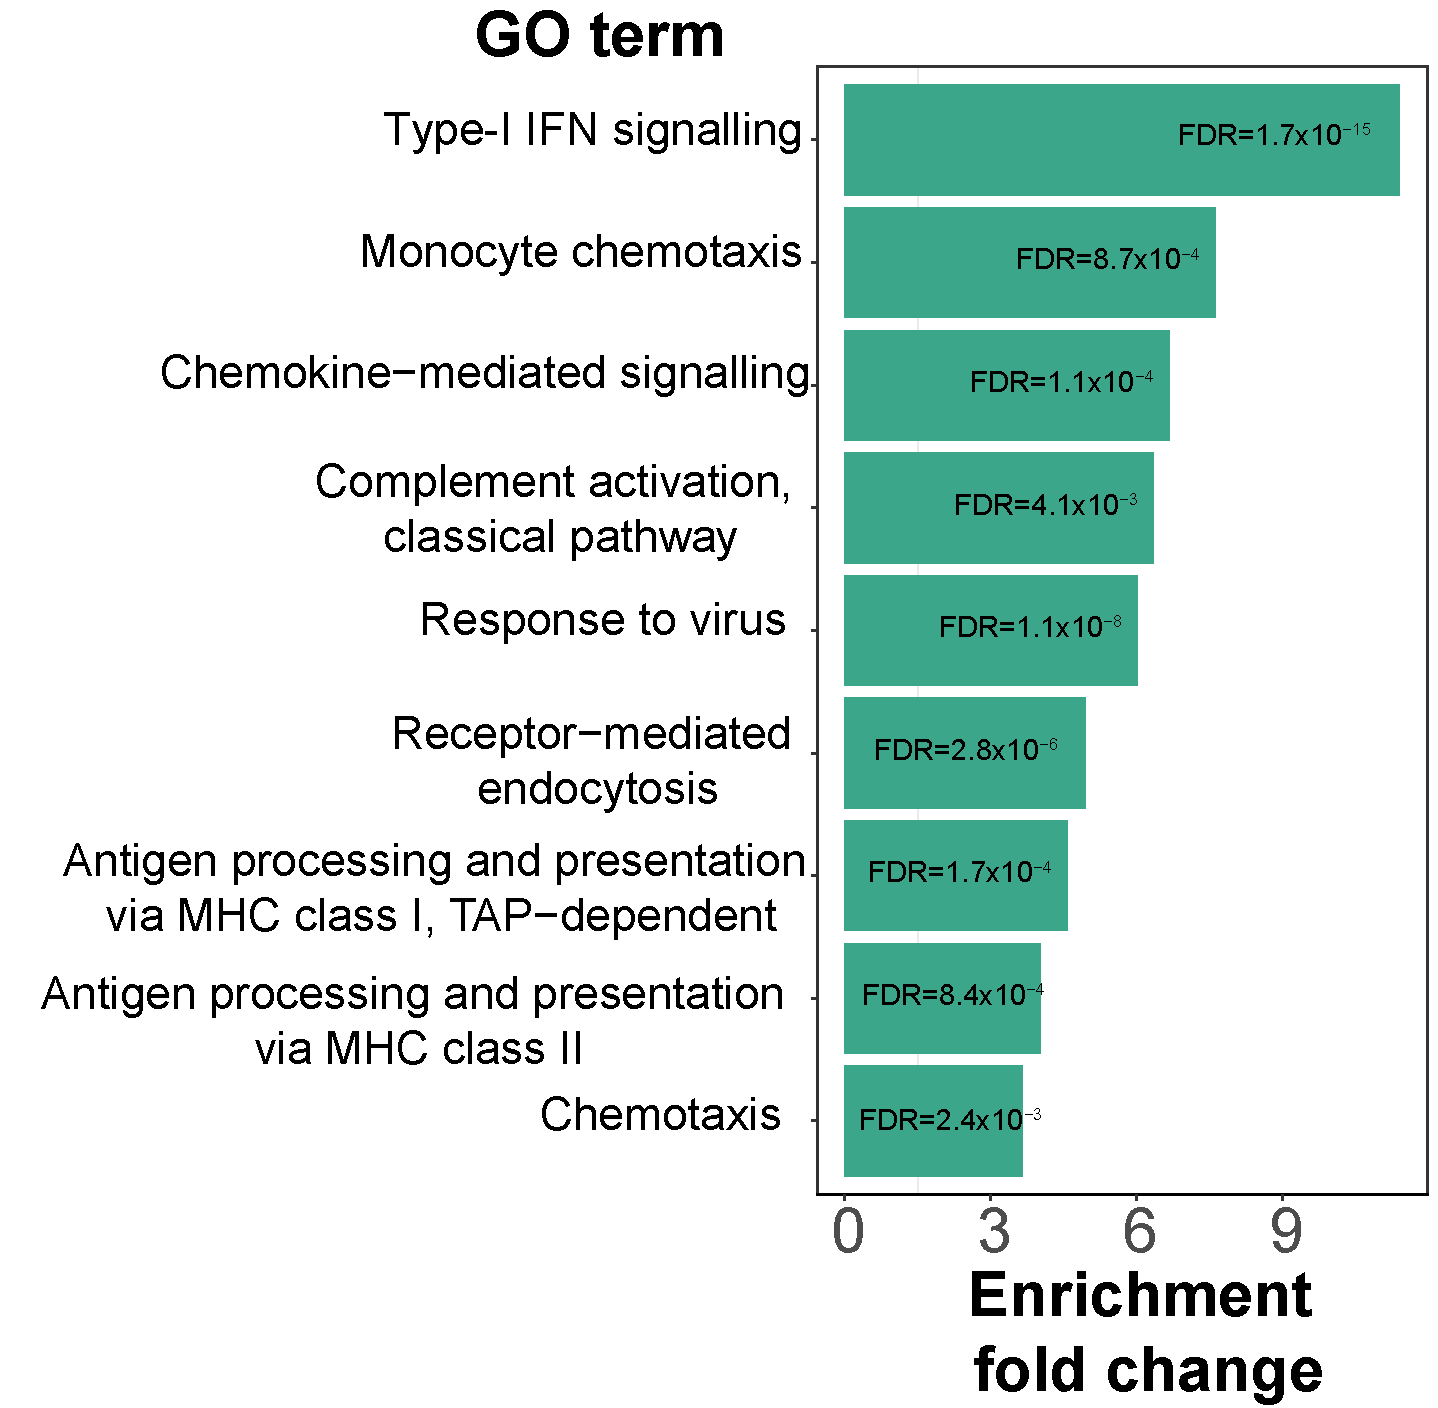
\includegraphics[width=\textwidth]{./Results3/pdfs/PSA_scanpy_single_cell_cluster_1_upregulated_GO_barplot_reduced}
		\caption{}
	\end{subfigure}
	~
	\begin{subfigure}[b]{0.50\textwidth} 
		%the [b] prevents offset in subcaptions
		\centering
		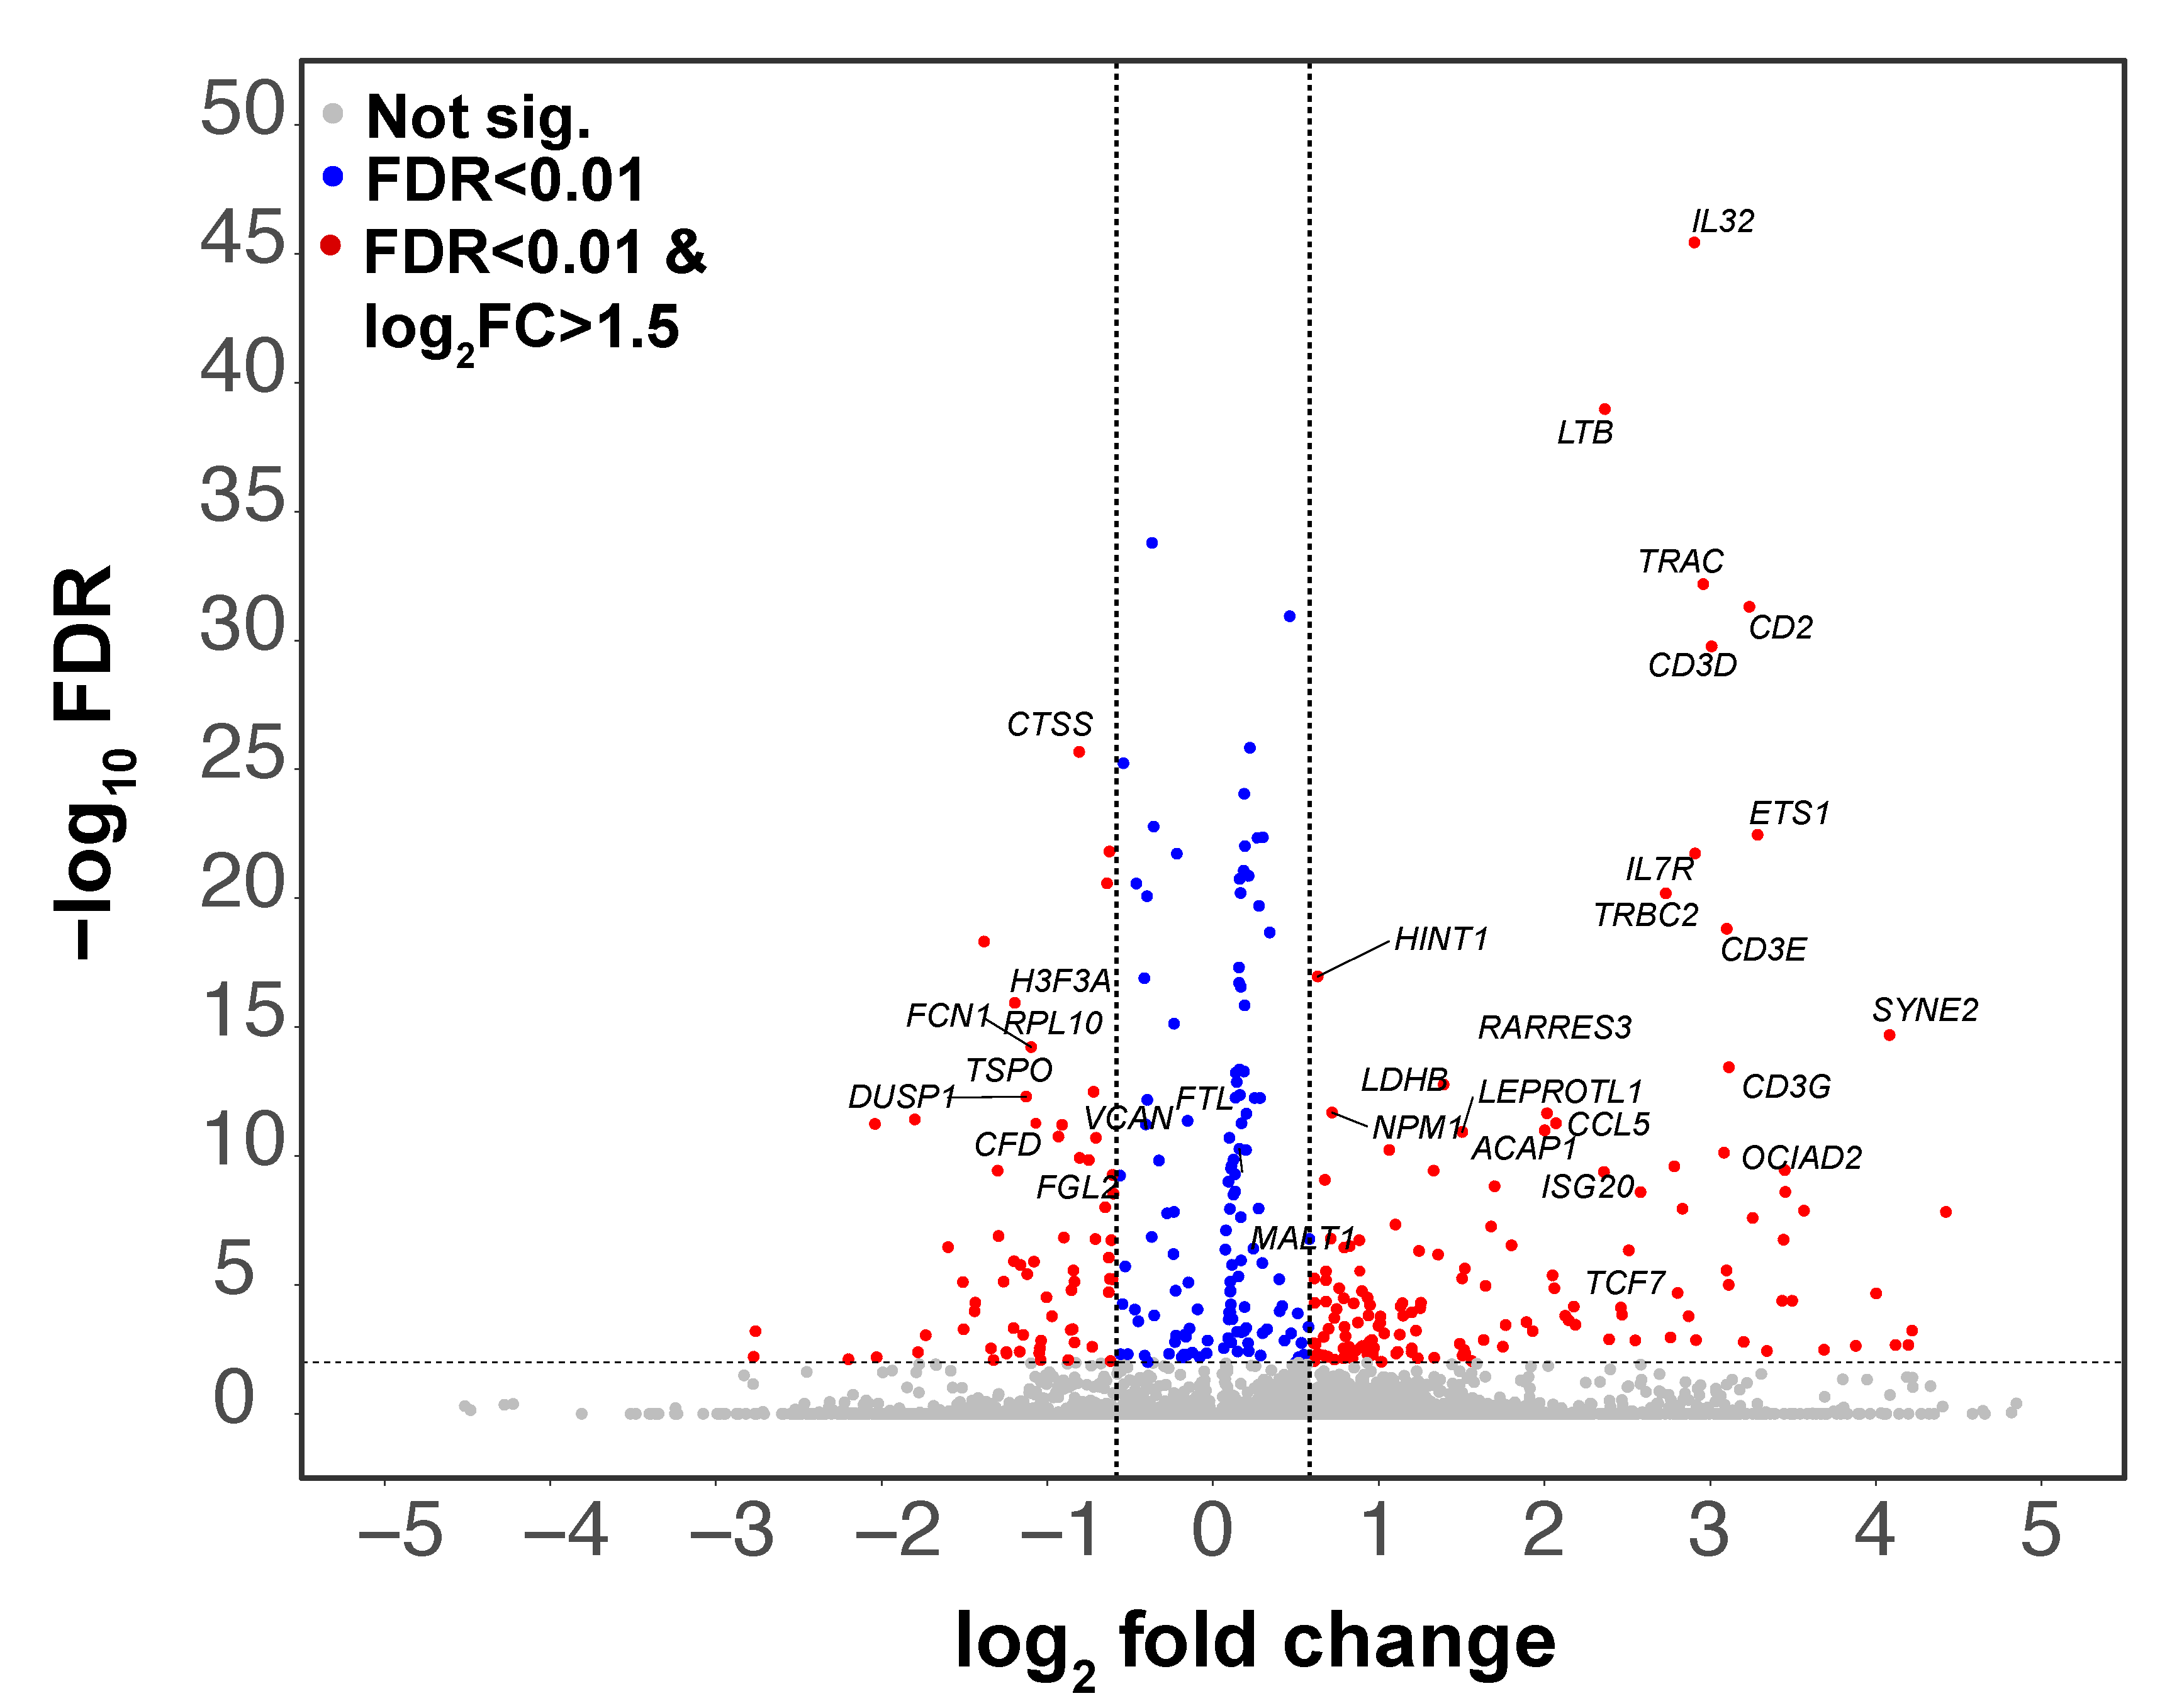
\includegraphics[width=\textwidth]{./Results3/pdfs/PSA_scanpy_single_cell_cluster_4_volcano_plot}
		\caption{}
	\end{subfigure}%
	~
	\begin{subfigure}[b]{0.50\textwidth} 
		%the [b] prevents offset in subcaptions
		\centering
		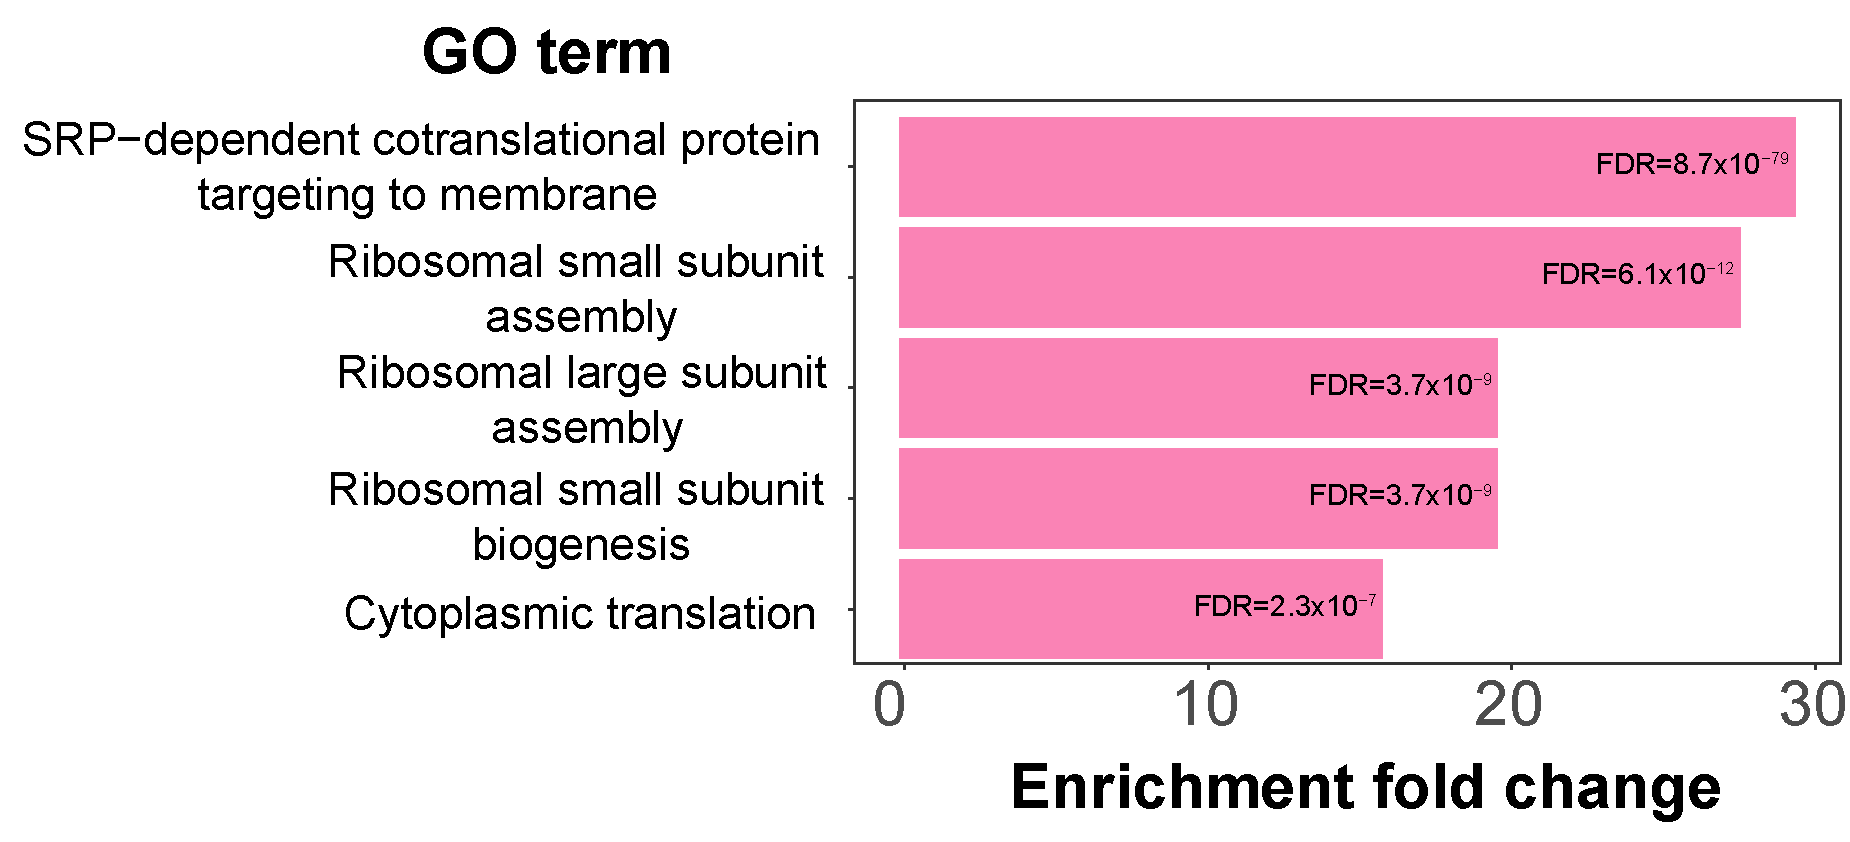
\includegraphics[width=\textwidth]{./Results3/pdfs/PSA_scanpy_single_cell_cluster_4_upregulated_GO_barplot}
		\caption{}
	\end{subfigure}%
	\caption[Functional characterisation of the MC-1 and MC-4 CD14$^+$ PsA monocyte subpopulations.]{\textbf{Functional characterisation of the MC-1 and MC-4 CD14$^+$ PsA monocyte subpopulations.} (A) Barplot illustrating the top Gene Ontology (GO) terms enriched for significantly up-regulated (FDR$<$0.01 and fold change$>$1.5) unique genes in the MC-1 cluster. (B) Volcano plots showing the differentially expressed genes in the MC-4 cluster when compared to the rest of CD14$^+$ monocytes interrogated by scRNA-seq. The significance (log$_{10}$FDR) of the differential expression (y-axis) is plotted against the log${_2}$fold change. Genes are coloured based on FDR and log$_{2}$fold changes and some of the top significant genes are labelled. (C) Barplot illustrating the top GO terms enriched for the significantly up-regulated genes (FDR$<$0.01) identified in the MC-4 cluster.}
\label{figure:PsA_scRNAseq_MC1_MC2_characterisation}
\end{figure}

\subsection{Identification of additional pathways dysregulated between  synovial fluid and peripheral blood CD14$^+$ monocytes using scRNA-seq data }
Differential gene expression between the CD14$^+$ monocytes from the two tissues was conducted to explore genome-wide differences that could complement the restricted qPCR analysis and serve as validation, since two out of the three PsA patients included in the single-cell analysis were different from the ones used for the qPCR analysis. A total of 1,275 genes were differentially expressed at an FDR$<$0.01 and fold change$>$1.5 between synovial fluid and peripheral blood (778 and 497 up- and down-regulated, respectively (Figure \ref{figure:PSA_monocytes_scanpy_single_cell_volcano_and_qPCR_ATAC_correlation}A). Out of the 72 DEGs identified by qPCR, 38 were also differentially expressed (FDR$<$0.01) by scRNA-seq analysis (32 when further restricting on fold change$>$1.5), including those showing  the largest changes between tissues, such as \textit{SPP1}, \textit{FN1}, \textit{S100A12} or \textit{FOS} (Figure \ref{figure:PSA_monocytes_scanpy_single_cell_volcano_and_qPCR_ATAC_correlation}B). 


Pathway enrichment analysis using the scRNA-seq significant DEGs (FDR$<$0.01 and fold-change$>$1.5) between synovial fluid and peripheral blood PsA monocytes confirmed enrichment for the chemokine signalling and NOD-like receptor pathways, previously reported by the qPCR array data (Figure \ref{tab:PSA_scRNAseq_enriched_pathways}). Up-regulation in synovial fluid CD14$^+$ monocytes of chemokines (including \textit{CCL18}, \textit{CCL2}, \textit{CCL3}, \textit{CCL4}, \textit{CCL8} and \textit{CXCL10}) and chemokine receptors (\textit{CCR1} and \textit{CCR5}) was consistent with the qPCR analysis and also revealed new members dysregulated between the two tissues. Additional genes of NOD-like receptor signalling pathways not interrogated by qPCR array that contributed to enrichment in this analysis included down-regulation of the negative regulators of the inflammasome \textit{CARD8} and \textit{NLRP12} (also a negative regulators of NF-$\kappa$B) \parencite{Mao2018,Williams2005}. Interestingly, the NOD-like receptor \textit{NLRP1} and caspase-1 (\textit{CASP1}), required for assembly of the inflammasome were down-regulated in PsA synovial fluid CD14$^+$ monocytes compared to peripheral blood.

Other relevant enriched pathway identified in this analysis included IFN and IFN-$\gamma$ signalling, MHC-II antigen presentation, complement cascade, apoptosis and osteoclast differentiation (Figure \ref{tab:PSA_scRNAseq_enriched_pathways}). The relevance of IFN signalling in the synovium was consistent with the up-regulation of IFN regulated genes in the MC-1 cluster, and was also driven by up-regulation of the TF \textit{STAT1} in synovial fluid CD14$^+$ monocytes. Enrichment of the apoptosis pathway was driven by down-regulation of positive regulators, such as the TFs \textit{FOS} and \textit{APAF1}, \textit{PRKCB} and \textit{TNFSF10}, and up-regulation of inhibitors, including \textit{BCL2}, \textit{BCL2A1} and \textit{BCL2L1}, in synovial fluid compared to peripheral blood CD14$^+$ monocytes. This may suggest an increased resistance to apoptosis by PsA synovial fluid monocytes. Moreover, CD14$^+$ monocytes from the synovium showed large up-regulation of the \textit{TNFRSF11A} (also known as \textit{RANK}) (fold change=26.5, Figure \ref{figure:PSA_monocytes_scanpy_single_cell_volcano_and_qPCR_ATAC_correlation}A) involved in monocytes differentiation to osteoclasts and NF-$\kappa$B activation \parencite{Mensah2008}, and down-regulation of \textit{NCF1}, which impairs extracellular degradation of inflammatory mediators by neutrophil proteases \parencite{Schauer2014}.
                                      

Lastly, genome-wide comparison between the log$_2$fold changes for all the genes analysed by scRNA-seq expression and all the regions interrogated for differential chromatin accessibility between synovial fluid and peripheral blood only showed low correlation (R=0.162, p-value=2x10$^{-16}$) (Figure \ref{figure:PSA_monocytes_scanpy_single_cell_volcano_and_qPCR_ATAC_correlation}B), with 252 and 75 genes changing expression and chromatin accessibility in the same or opposite direction, respectively (significant enrichment, p-value=6.264x10$^-11$ Fisher exact test). For example, \textit{CCL2}, \textit{FN1} and \textit{FABP5} showed transcriptional up-regulation and were in the proximity of a synovial fluid open DAR (Figure \ref{figure:PSA_monocytes_scanpy_single_cell_volcano_and_qPCR_ATAC_correlation}C).


\subsection{Integration of mass cytometry differences in protein expression with chromatin accessibility and gene expression data in PsA CD14$^+$ monocytes.}
\label{cytof}

To determine the effect of chromatin accessibility and genes expression differences in CD14$^+$ monocytes between synovial fluid and peripheral blood at the protein level, mass cytometry was conducted by Dr Hussein Al-Mossawi and Dr Nicole Yager in collaboration with UCB. This analysis included the six samples with either paired ATAC/qPCR data or scRNA-seq analysis presented in this chapter (Table \ref{tab:PSA_datasets_per_sample}) and an additional four PsA patients recruited only for mass cytometry processing. Intra-cellular staining for relevant cytokines and chemokines was performed before and after treatment with BFA (blocker of protein transport) and enables identification of cells actively producing the protein of interest in the closest state to the physiological, without additional inflammatory stimuli (see Chapter \ref{ch:Mat}).

Amongst the measured proteins, TNF-$\alpha$, osteopontin (protein product of \textit{SPP1}), MCP-1 (protein product of \textit{CCL2}) and IP-10 (protein product of \textit{CXCL10}) were of particular interest as they showed transcriptional up-regulation in synovial fluid CD14$^+$ monocytes compared to peripheral blood and have a key role in pathological inflammation. In the three PsA patients processed for ATAC and qPCR mass cytometry expression in CD14$^+$ of TNF-$\alpha$, osteopontin, MCP-1 and IP-10 demonstrated a greater increase in cell staining for each cytokine after 6h of BFA treatment in CD14$^+$ monocytes from synovial fluid when compared to peripheral blood (Figure \ref{figure:PsA_monocytes_biaxial_TNFa_MCP1_osteopontin_IP10}).



\bigskip
\begin{figure}[H]
\centering
\begin{subfigure}[b]{0.45\textwidth}
\centering 
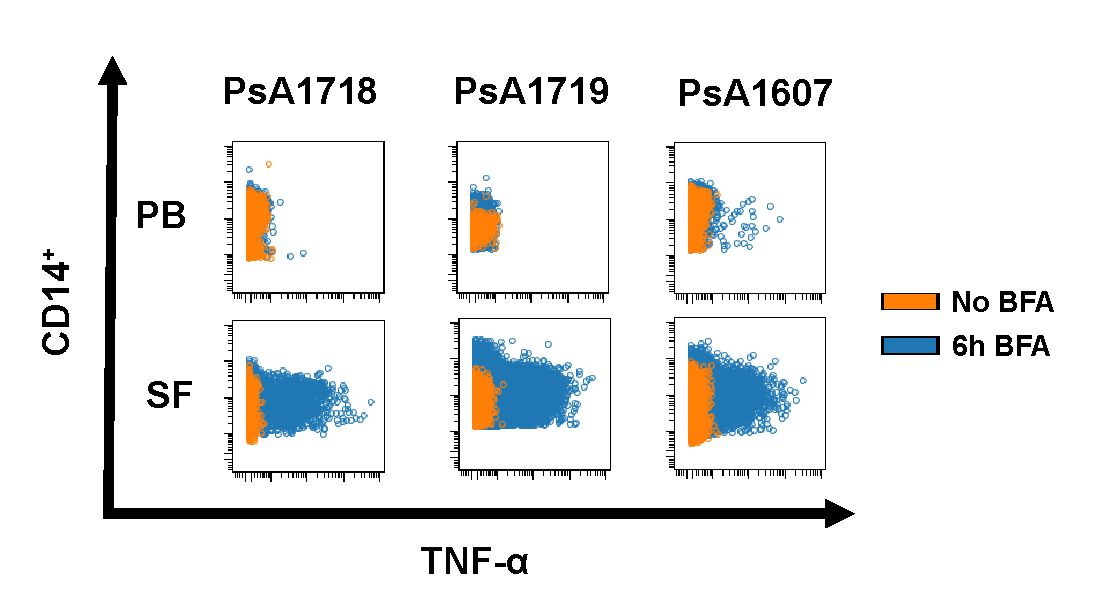
\includegraphics[width=\textwidth]{./Results3/pdfs/PSA_0h_6h_BFA_TNFa_mass_cytometry_PSA1718_PSA1719_PSA1607}
\caption{}
\end{subfigure}
~
\begin{subfigure}[b]{0.45\textwidth} 
%the [b] prevents offset in subcaptions
\centering
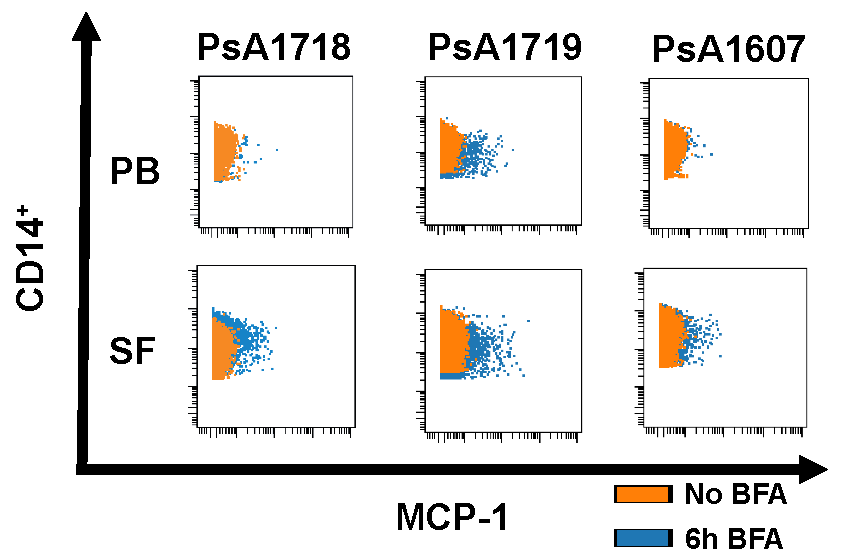
\includegraphics[width=\textwidth]{./Results3/pdfs/PSA_0h_6h_BFA_MCP1_mass_cytometry_PSA1718_PSA1719_PSA1607}
\caption{}
\end{subfigure}
\begin{subfigure}[b]{0.45\textwidth} 
%the [b] prevents offset in subcaptions
\centering
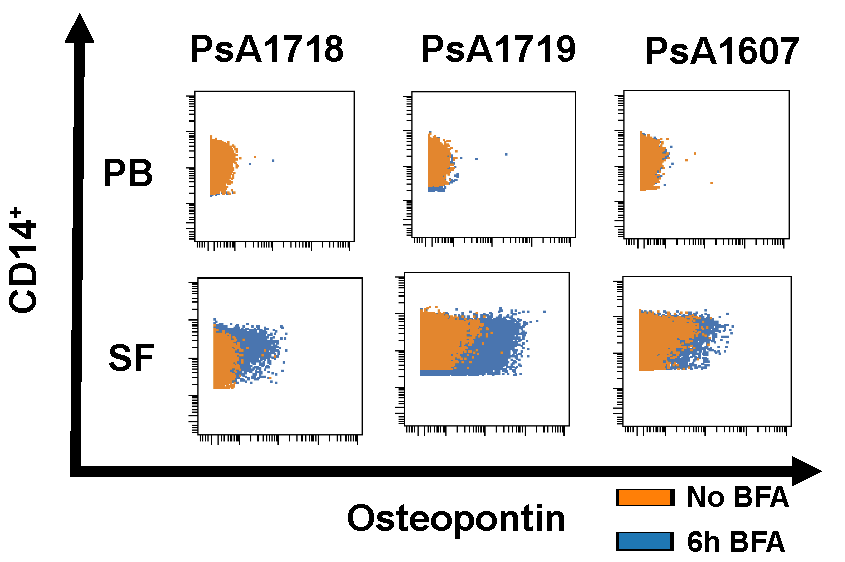
\includegraphics[width=\textwidth]{./Results3/pdfs/PSA_0h_6h_BFA_osteopontin_mass_cytometry_PSA1718_PSA1719_PSA1607}
\caption{}
\end{subfigure}%
\begin{subfigure}[b]{0.45\textwidth} 
%the [b] prevents offset in subcaptions
\centering
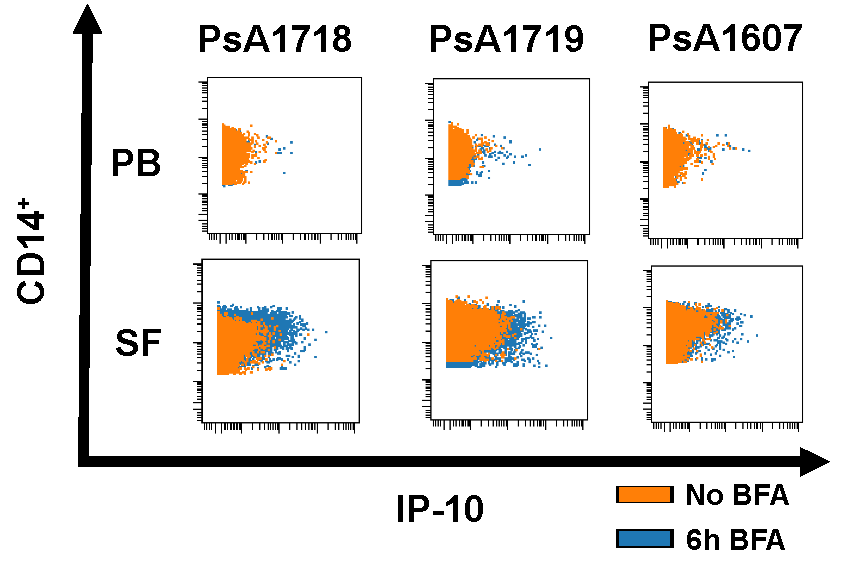
\includegraphics[width=\textwidth]{./Results3/pdfs/PSA_0h_6h_BFA_IP10_mass_cytometry_PSA1718_PSA1719_PSA1607}
\caption{}
\end{subfigure}
\caption[Biaxial representation of CD14$^+$ monocytes expressing TNF-$\alpha$, MCP-1, osteopontin and IP-10 in synovial fluid and peripheral blood before and after protein transport blockade with BFA using mass cytometry.]{\textbf{Biaxial representation of CD14$^+$ monocytes expressing TNF-$\alpha$, MCP-1, osteopontin and IP-10 in synovial fluid and peripheral blood before and after protein transport blockade with BFA using mass cytometry.} For each of the three PsA patients with ATAC and expression data, expression of the monocytes marker CD14$^+$ vs (y-axis) vs (A) TNF-$\alpha$, (B) MCP-1, (C) osteopontin or (D) IP-10 (x-axis) in matched synovial fluid and peripheral blood without protein transport blockade (blue dots) or after 6h of treatment with BFA (orange dots).}
\label{figure:PsA_monocytes_biaxial_TNFa_MCP1_osteopontin_IP10}
\end{figure}



%In order to validate this observation and also assess other cytokines of interest, mass cytometry was conducted in peripheral blood and synovial fluid from another ten PsA patients. This validation cohort included the patients for which scRNA-seq data was presented in this chapter (Table \ref{tab:PSA_datasets_per_sample}). As previously, percentage of CD14$^+$ monocytes producing TNF-$\alpha$ , MCP-1 (protein product of \textit{CCL2} and osteopontin (protein product of \textit{SPP1}) was computed as the difference between percentage of cells producing each of the cytokines before and after BFA treatment. The percentage of CD14$^+$ monocytes producing TNF-$\alpha$ was greater in synovial fluid compared to peripheral blood (p-value=0.048) (Figure \ref{figure:CyTOF_cytokines_validation_cohort} a), reinforcing the results from the previous cohort. Likewise, a larger percentage of CD14$^+$ monocytes producing osteopontin and MCP-1 (p-value=0.001 and p-value=0.003, respectively) were also observed in synovial fluid compared to peripheral blood (Figure \ref{figure:CyTOF_cytokines_validation_cohort} b and c), in line with the up-regulated expression of these two genes in synovial fluid compared to peripheral blood in bulk CD14$^+$ monocytes and in the CC-mixed scRNA-seq cluster. The percentage of cells producing cytokines in synovial fluid was particularly moderate for TNF-$\alpha$ and MCP-1, not exceeding of 1.8 and 3, respectively, for the majority of the PsA samples (Figure \ref{figure:CyTOF_cytokines_validation_cohort} a and c). However, one of the patients (PSA1505) appeared to have particularly higher percentage of synovial fluid CD14$^+$ monocytes producing all three cytokines when compared to the rest of the patients in the cohort. Although no justification was found to remove this sample, the statistical significance (p-value$<$0.05) in the differences found between percentage of cell producing TNF-$\alpha$, MCP-1 and osteopontin in synovial fluid versus peripheral blood remained when repeating the analysis in absence of PSA1505.

The increment in percentage of CD14$^+$ monocytes producing each of these four inflammatory mediators after blocking protein transport with BFA treatment was determined for each of the PsA patients in each compartment (peripheral blood and synovial fluid). For each immune mediator and compartment, this increment was calculated as the difference between the percentage of cells with positive staining after 6h BFA treatment and the percentage of positive staining cells at 0h (in absence of BFA incubation).The increment in the percentage of CD14$^+$ monocytes producing TNF-$\alpha$ was significantly greater in synovial fluid compared to peripheral blood (Wilcoxon signed-rank test, p-value=0.048) (Figure \ref{figure:CyTOF_cytokines_validation_cohort}A), in line with enrichment of SF open DARs nearby genes of the NF-$\kappa$B signalling pathway, the enrichment of DEGs for the TLR and NOD-like signalling pathways and the qPCR up-regulated expression of \textit{TNF} in synovial CD14$^+$ monocytes. % as well as with increased expression in synovial fluid of a number of genes in the TLR and NOD-like signalling leading to enhanced NF$\kappa$B activation and cytokine production. 
Likewise, greater percentage of CD14$^+$ monocytes producing osteopontin, MCP-1 and IP-10 (Wilcoxon signed-rank test p-value=0.001, p-value=0.003 and p-value=0.001, respectively) after BFA treatment were observed in synovial fluid compared to peripheral blood (Figure \ref{figure:CyTOF_cytokines_validation_cohort}B, C and D). The greater increase in the percentage of cells producing MCP-1 and osteopontin in synovial fluid monocytes was in line with the up-regulated expression of these two genes in synovial fluid compared to peripheral blood by qPCR and scRNA-seq analysis. Importantly, PsA1807 showed particularly higher percentage of synovial fluid CD14$^+$ monocytes producing all four molecules after BFA treatment when compared to the other patients in the cohort (Figure \ref{figure:CyTOF_cytokines_validation_cohort}A, B and C in pink). Nevertheless, the differences in the increment of positive cells after BFA treatment between synovial fluid and peripheral blood still remained significant (p-value<0.05) when removing PsA1807 from the analysis, also in the case of TNF-$\alpha$ and MCP-1 (showing more moderate differences than IP-10 and osteopontin).



\bigskip
\begin{figure}[H]
\centering
\begin{subfigure}[b]{0.40\textwidth}
\centering 
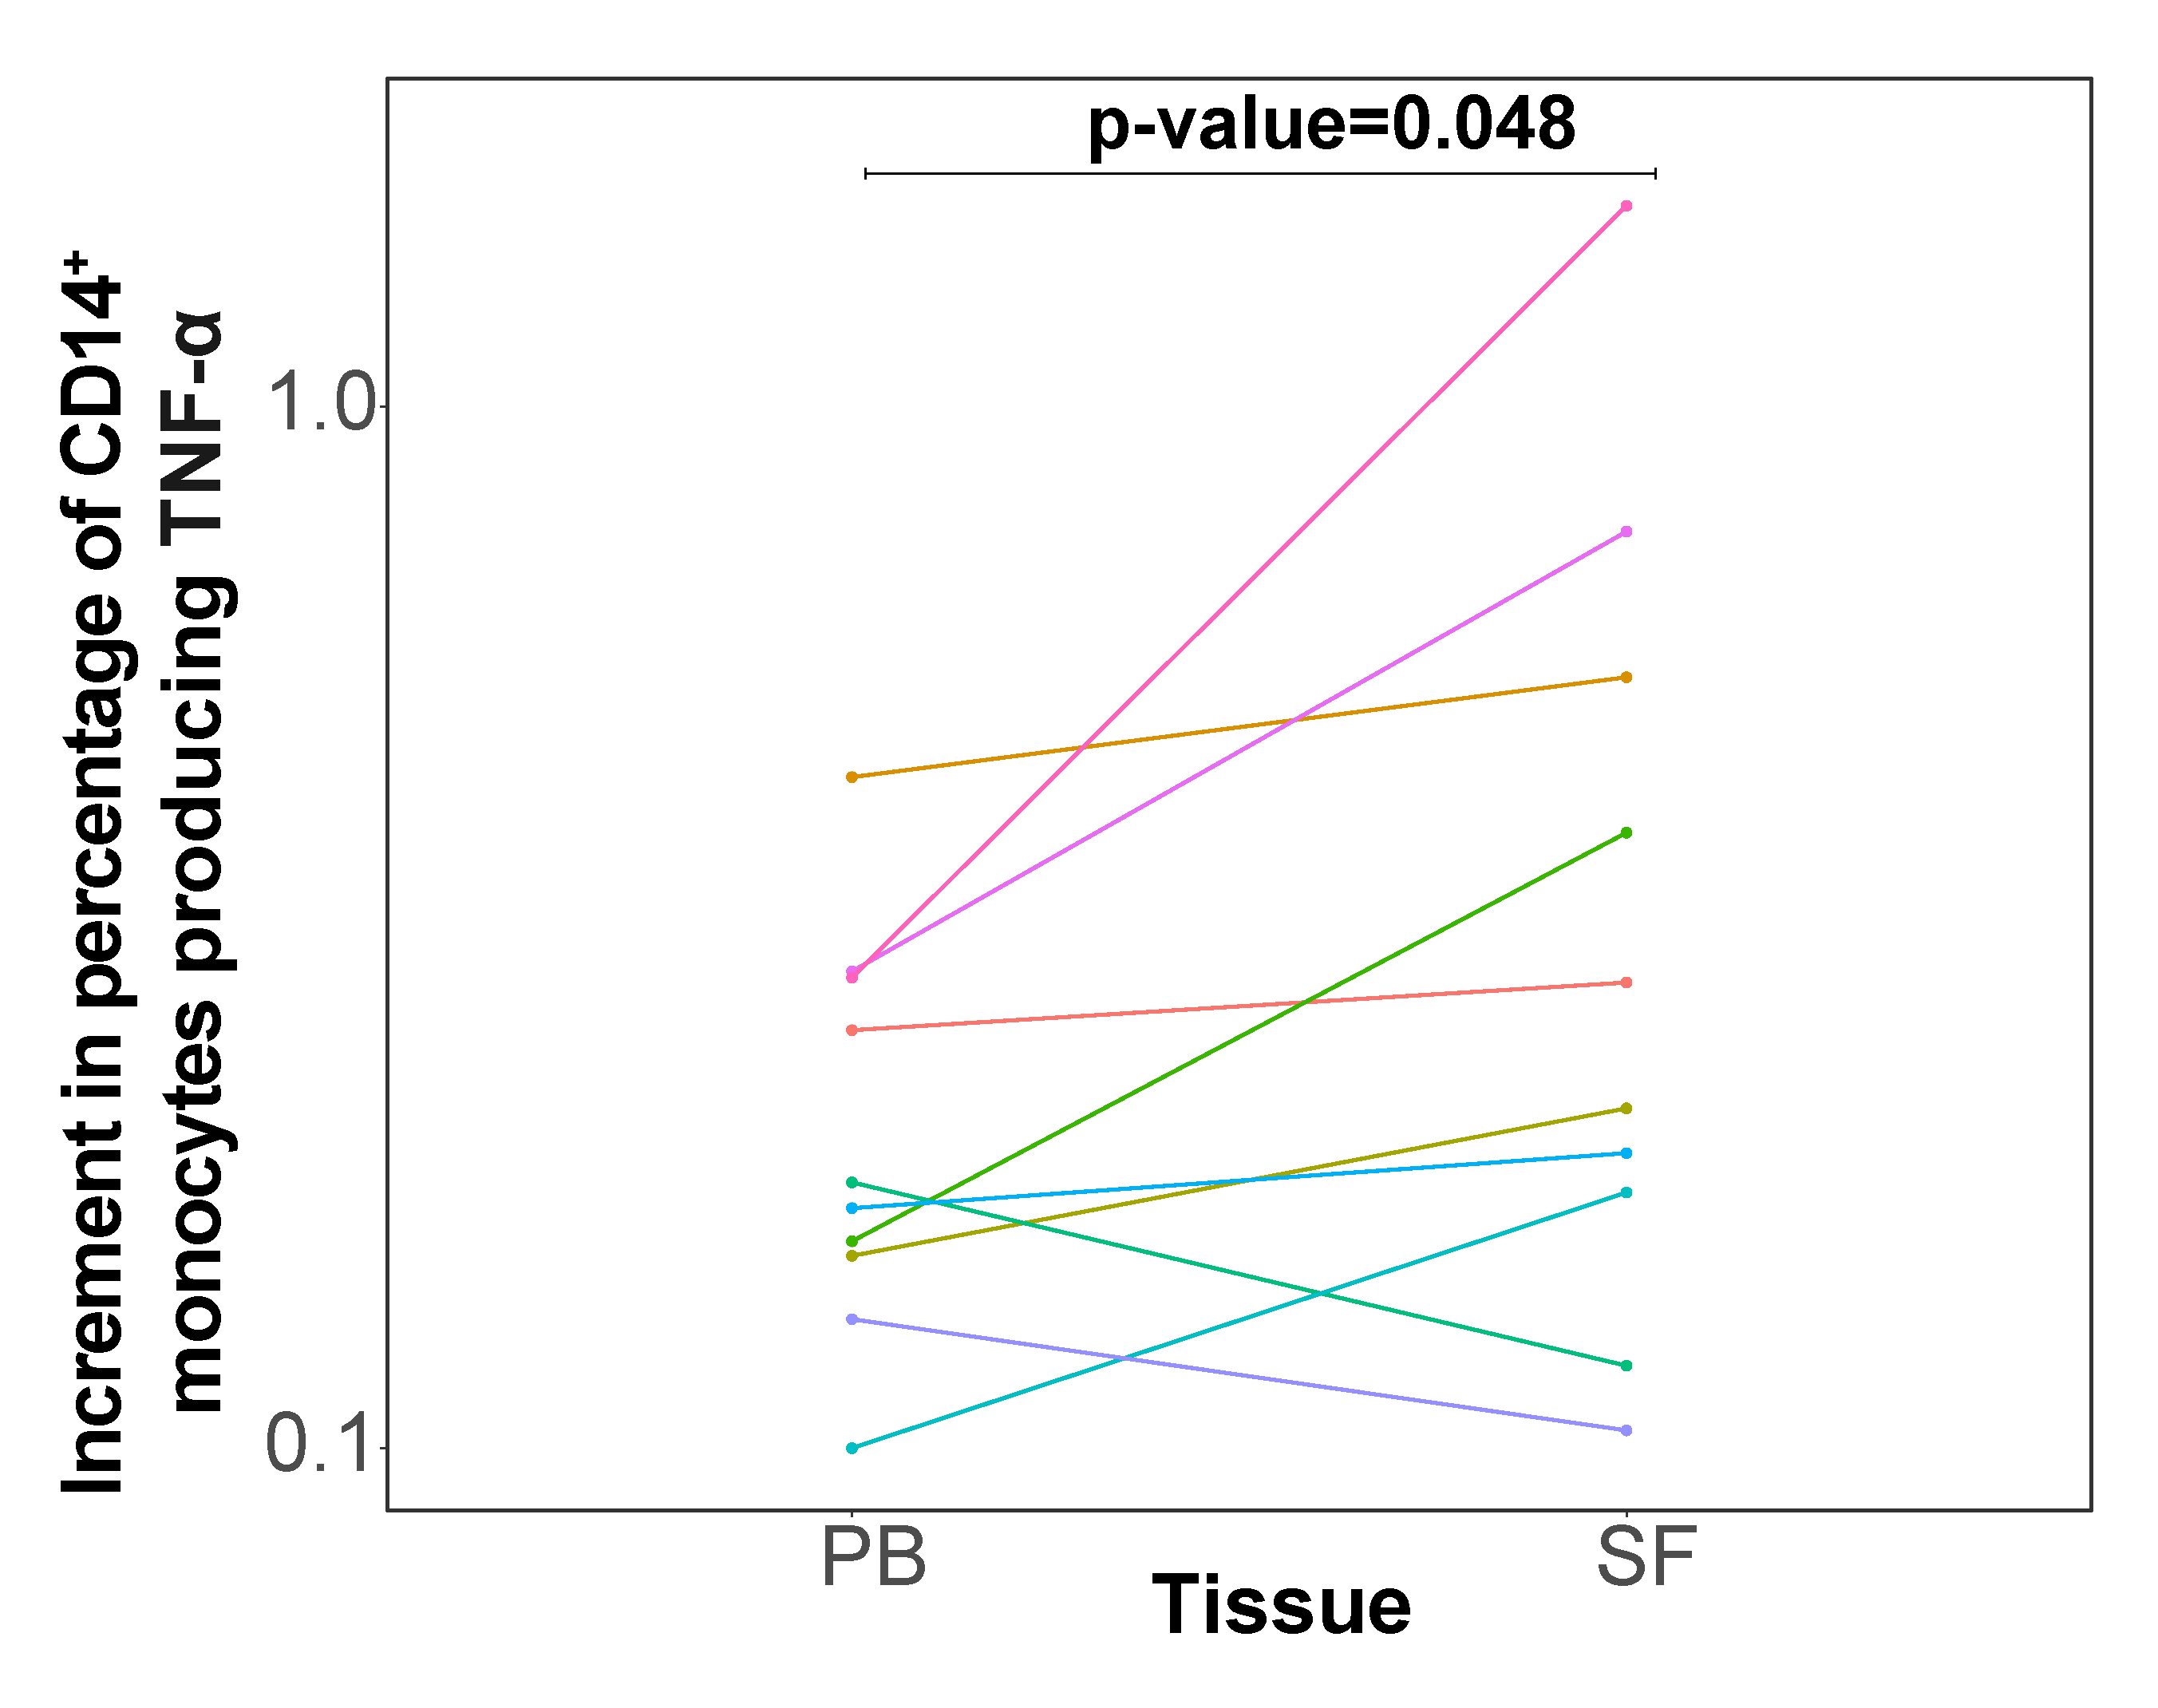
\includegraphics[width=\textwidth]{./Results3/pdfs/CyTOF_validation_cohort_TNFa_percentage_log10_scale}%
\caption{}
\end{subfigure}%
~
\begin{subfigure}[b]{0.40\textwidth}
\centering 
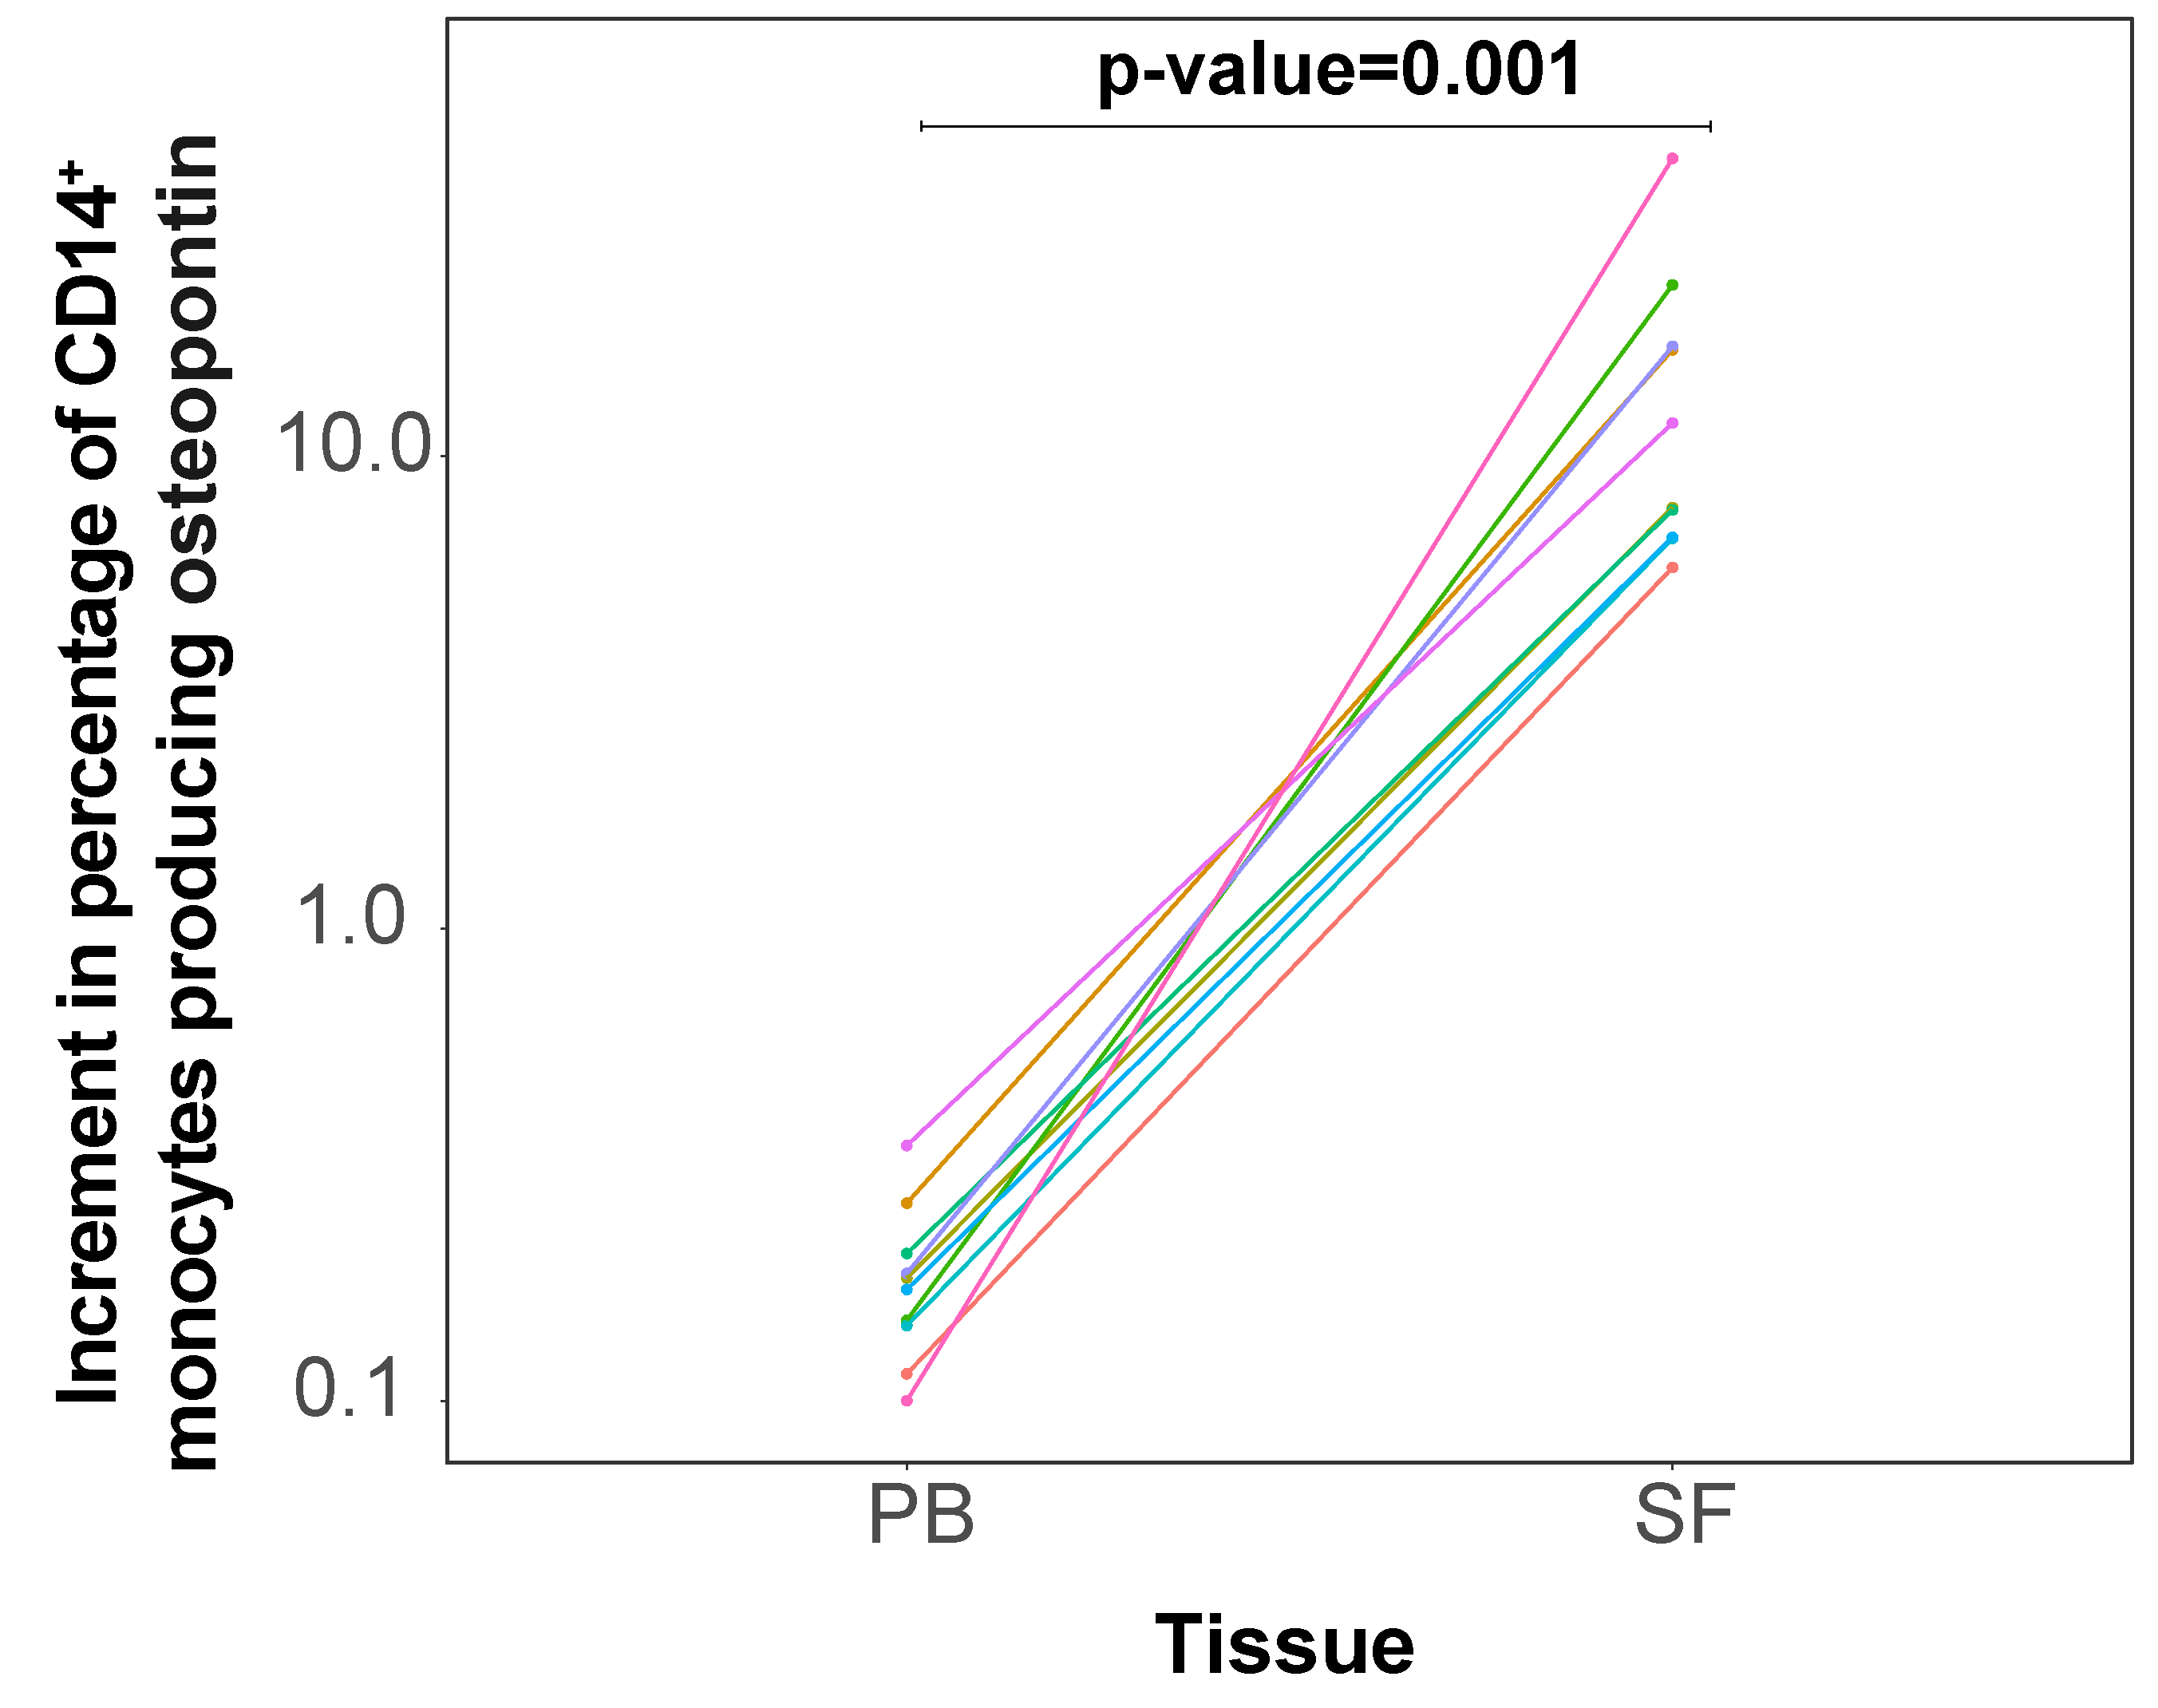
\includegraphics[width=\textwidth]{./Results3/pdfs/CyTOF_validation_cohort_osteopontin_percentage_log10_scale}
\caption{}
\end{subfigure}
~
\begin{subfigure}[b]{0.40\textwidth} 
%the [b] prevents offset in subcaptions
\centering
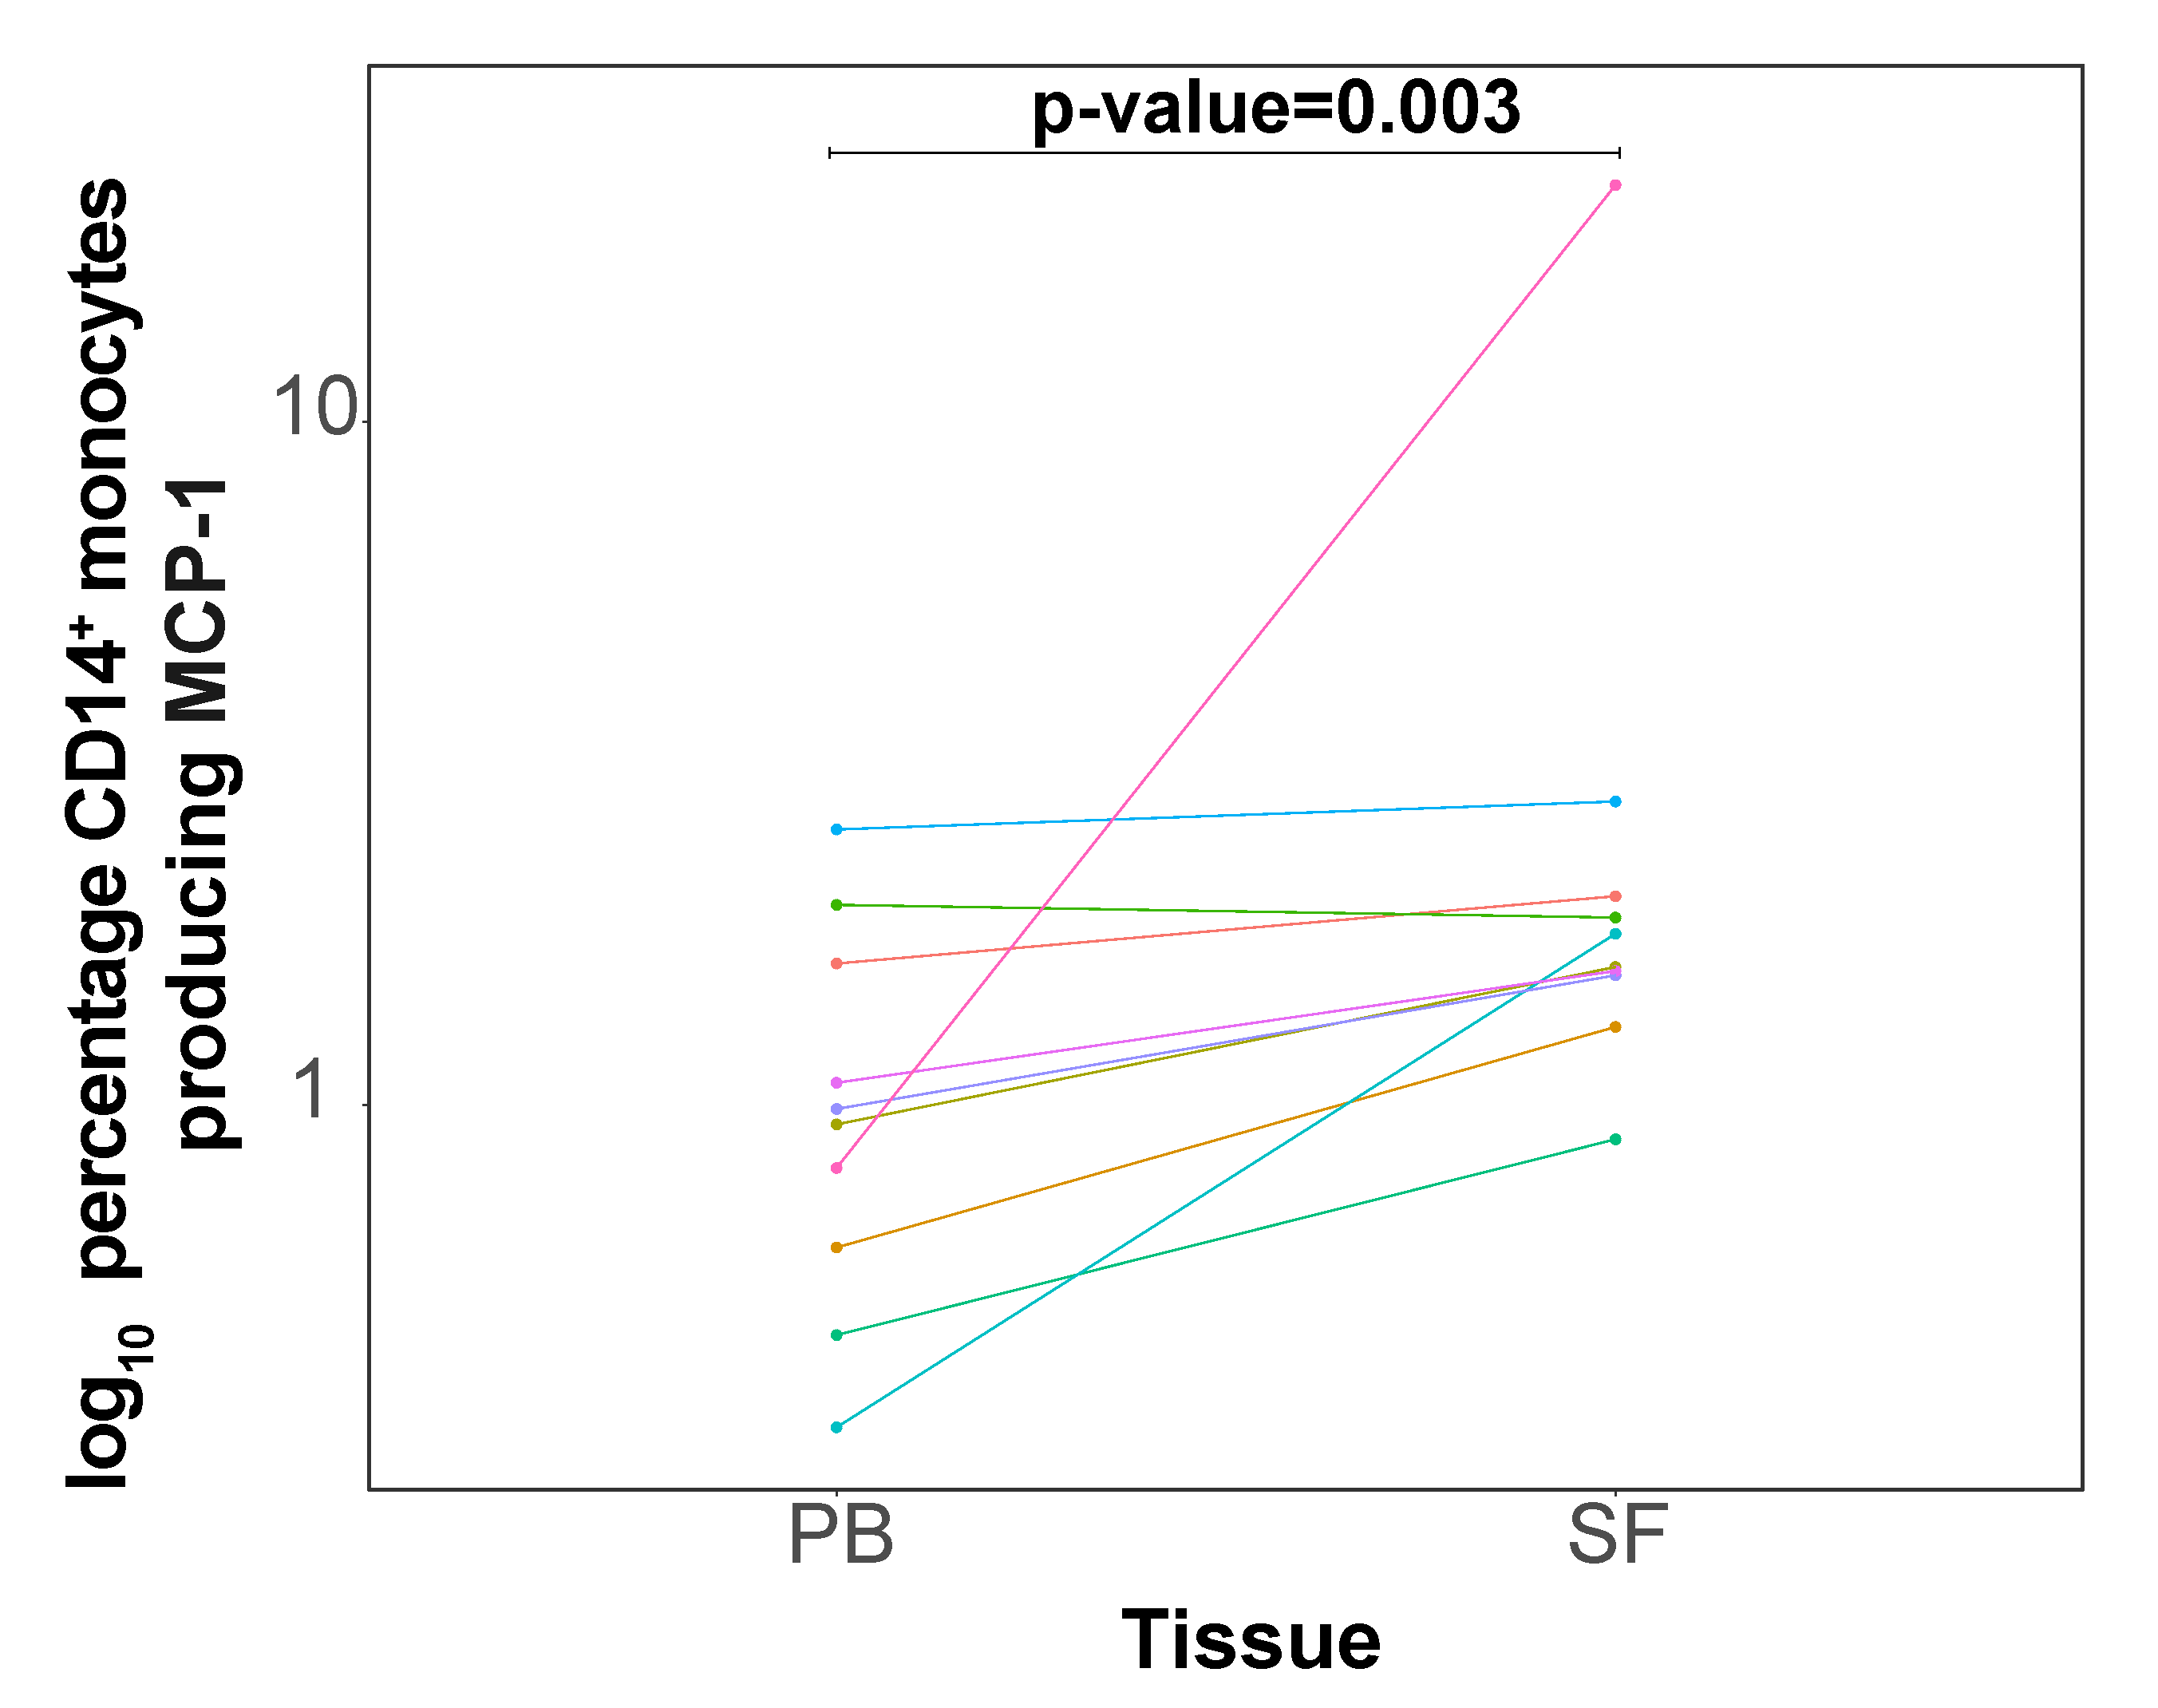
\includegraphics[width=\textwidth]{./Results3/pdfs/CyTOF_validation_cohort_CCL2_percentage_log10_scale}
\caption{}
\end{subfigure}%
~
\begin{subfigure}[b]{0.40\textwidth} 
%the [b] prevents offset in subcaptions
\centering
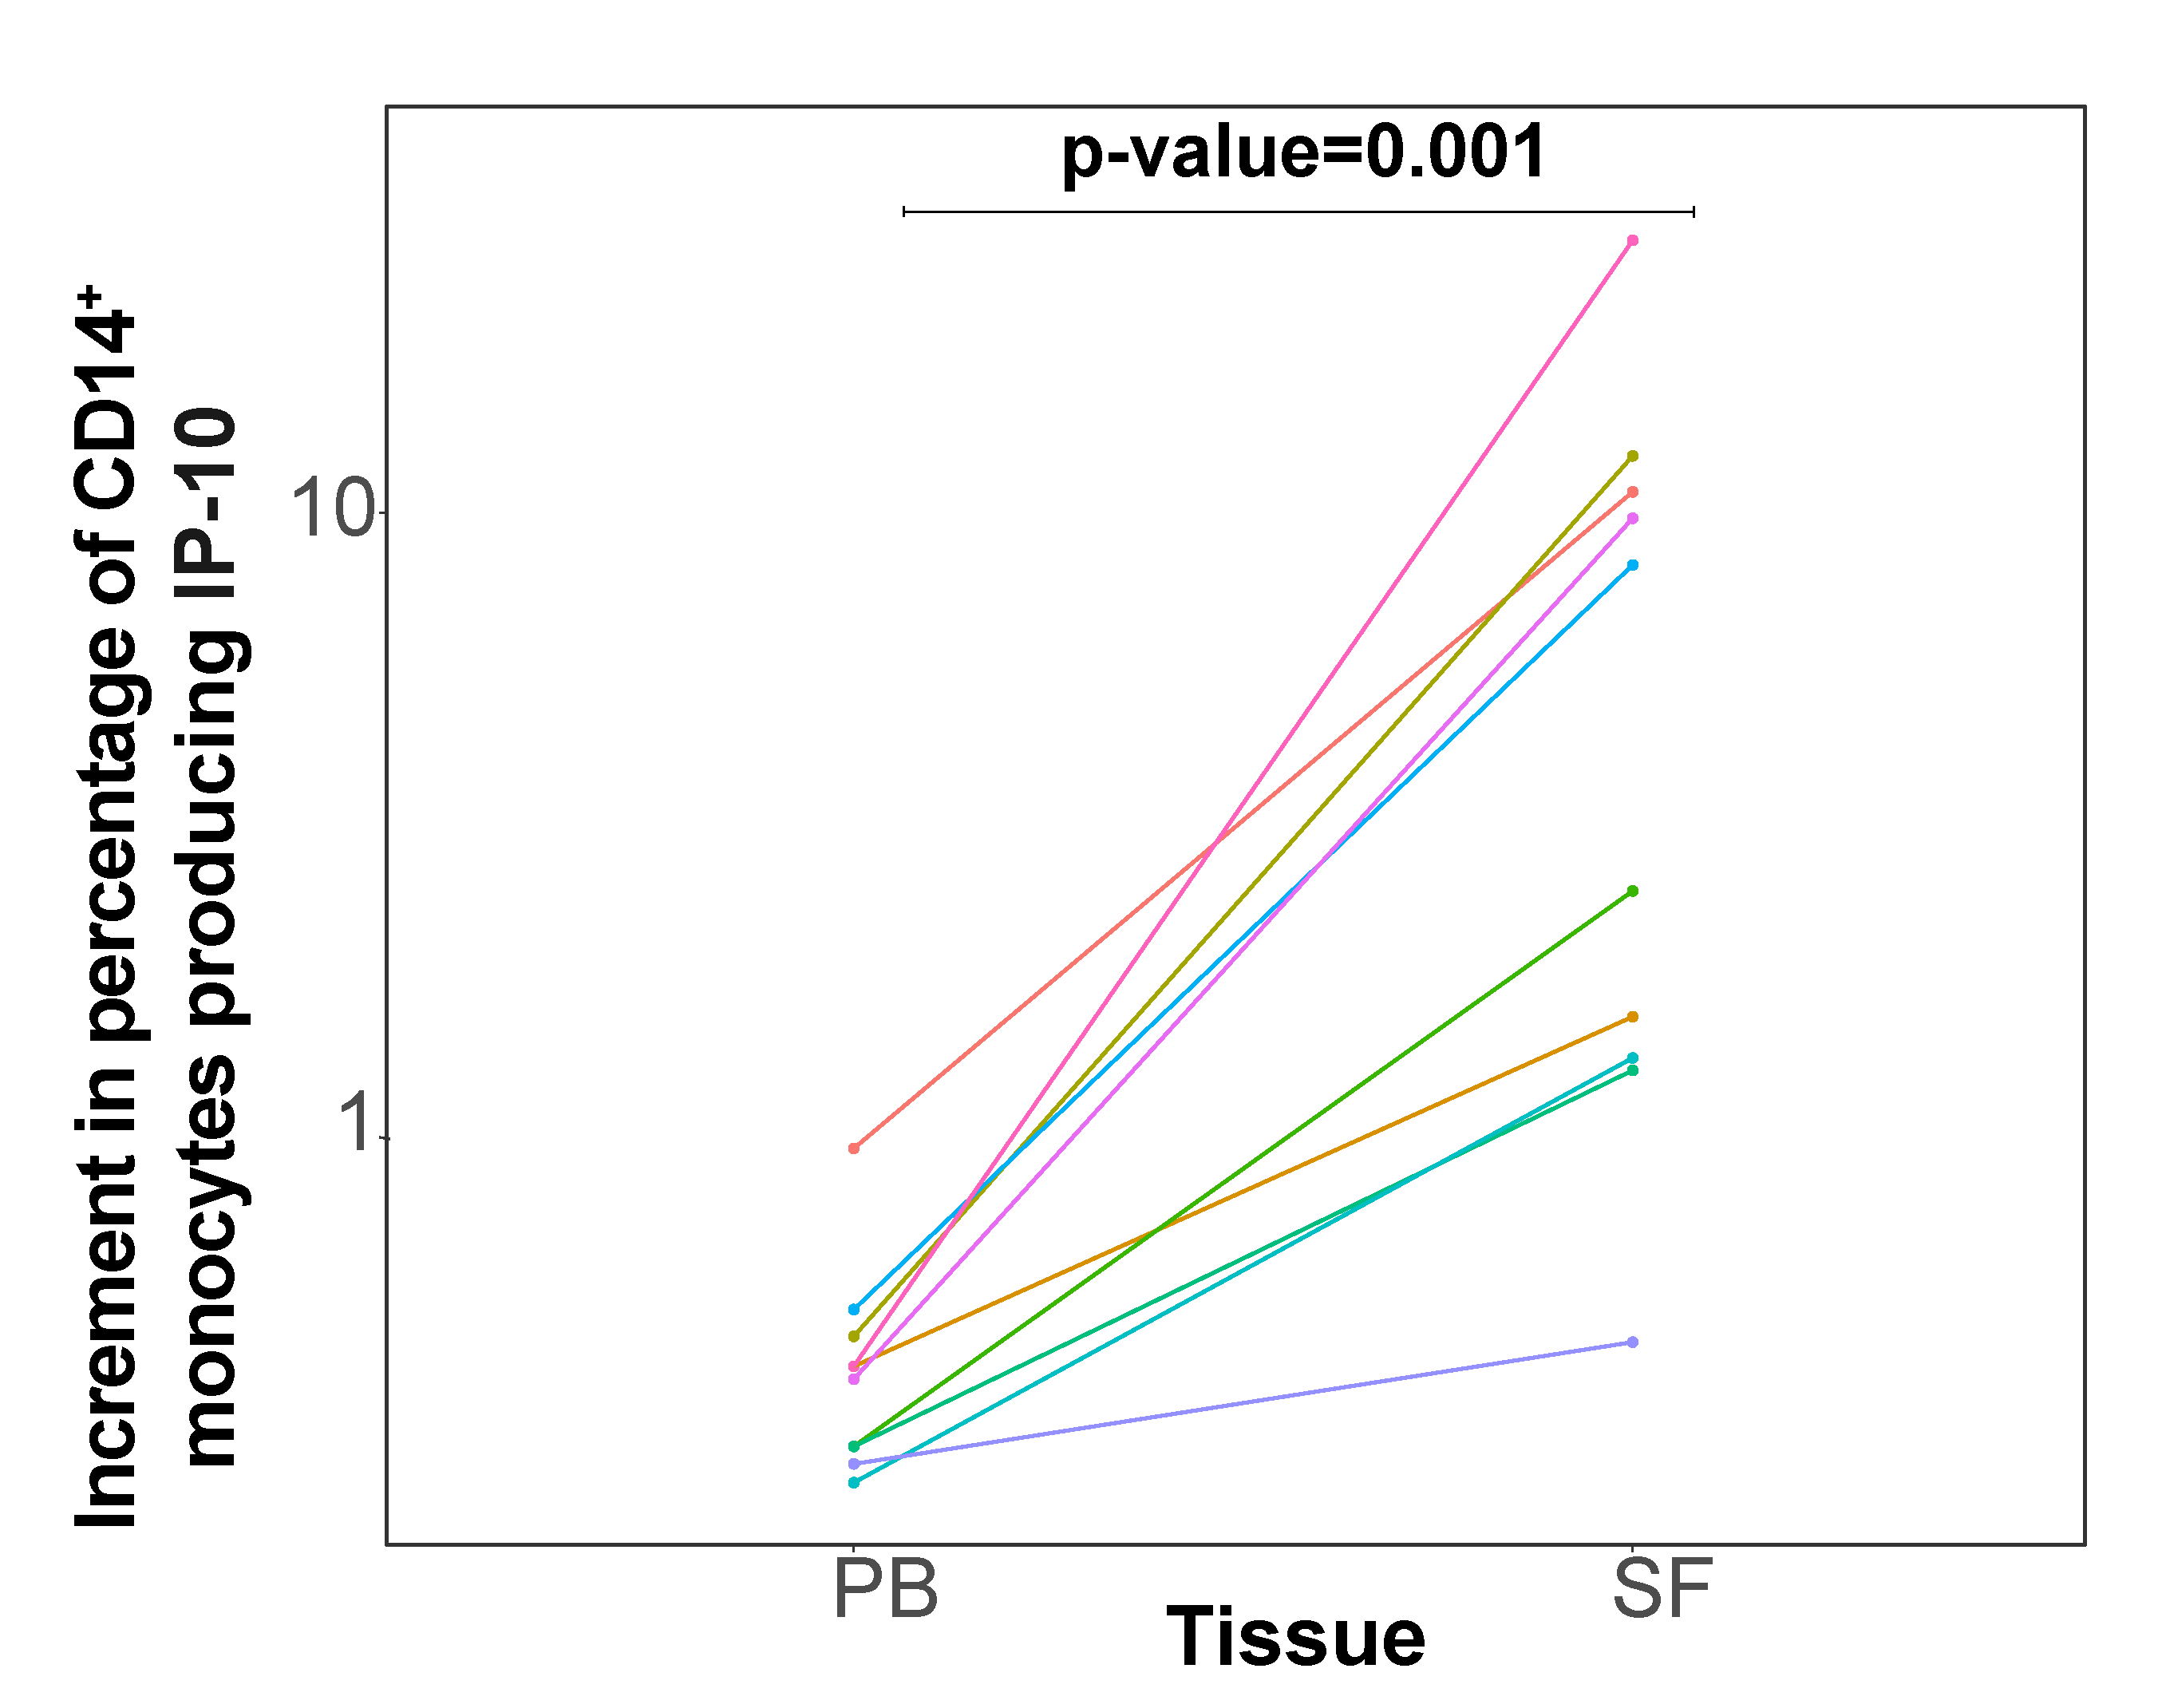
\includegraphics[width=\textwidth]{./Results3/pdfs/CyTOF_validation_cohort_IP10_percentage_log10_scale}
\caption{}
\end{subfigure}
~
\begin{subfigure}[b]{0.65\textwidth} 
%the [b] prevents offset in subcaptions
\centering
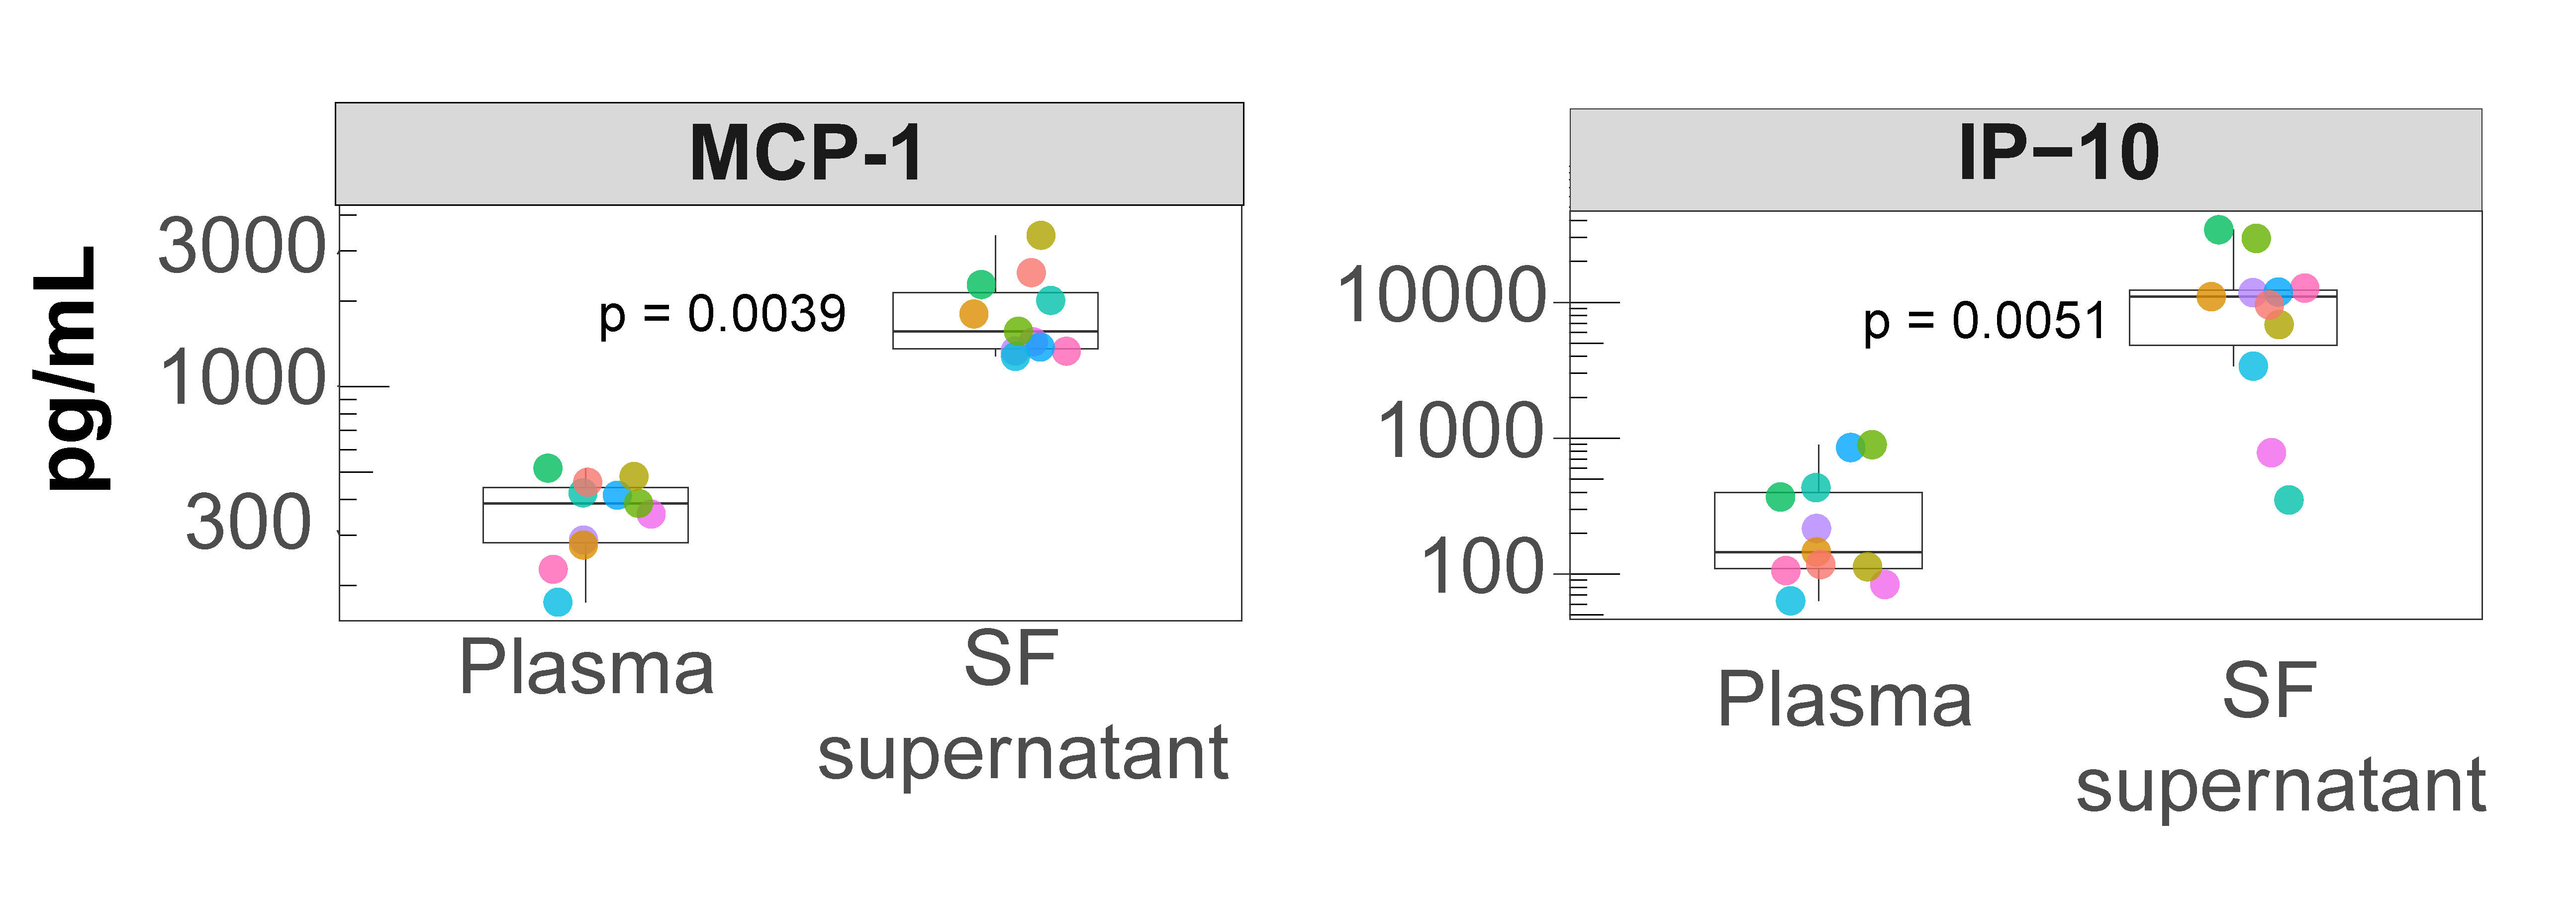
\includegraphics[width=\textwidth]{./Results3/pdfs/ELISA_MCP1_IP10_boxplot_10_PsA_SF_plasma}
\caption{}
\end{subfigure}
\caption[Increment in the percentage of CD14$^+$ monocytes producing TNF-$\alpha$, osteopontin, MCP-1 and IP-10 after BFA treatment in synovial fluid and peripheral blood.]{\textbf{Increment in the percentage of CD14$^+$ monocytes producing TNF-$\alpha$, osteopontin, MCP-1 and IP-10 after BFA treatment in synovial fluid and peripheral blood.} The increment in the percentage of CD14$^+$ monocytes producing (A) TNF-$\alpha$, (B) osteopontin , (C) MCP-1 and (D) IP-10 in synovial fluid and peripheral blood are shown for each of the ten PsA samples assayed by mass cytometry. In each sample and tissue, the increment in the percentage of cells producing each of the cytokines is calculated as the difference in positive cells for the relevant cytokine before and after BFA treatment (6h minus 0h). Axis are transformed into a log$_{10}$ scale. (E) Boxplots illustrating the concentration in pg/mL (x-axis log$_{10}$ scale) of MCP-1 and IP-10 measured in supernatant from synovial fluid and plasma from peripheral blood of ten PsA patients using enzyme-linked immunosorbent assay (ELISA). The statistical significance of the differences between synovial fluid and peripheral blood was determined using Wilcoxon signed-rank test. SF=synovial fluid; PB=peripheral blood.}
\label{figure:CyTOF_cytokines_validation_cohort}
\end{figure}




%\subsubsection{\textit{CCL2}-\textit{CCR2} signalling: an example of multi-omics correlation}

The differences in the percentage of CD14$^+$ monocytes producing MCP-1 and IP-10 between synovial fluid and peripheral blood were of particular interest due to correlating changes in chromatin accessibility, gene expression and protein production. A statistically significant synovial fluid open DAR was found in CD14$^+$ monocytes upstream \textit{CCL2} gene (Figure \ref{figure:PsA_10X_qPCR_ATAC_CD14_CCL2_CXCL10}A). Similarly, two synovial fluid open DARs were also identified upstream and at the promoter of the \textit{CXCL10} gene (Figure \ref{figure:PsA_10X_qPCR_ATAC_CD14_CCL2_CXCL10}B)


%, whereas no significant changes were observed for mCD4$^+$ and mCD8$^+$ in this data from the same patients (Figure \ref{figure:PSA_PCR_array_vulcano_plots} a, b, c and Table \ref{tab:PSA_gene_expression_ATAC_overlap}). Up-regulation of \textit{CCL2} was not found in peripheral blood CD14$^+$ monocytes compared to PsA patients and healthy controls, being defined as one of the tissue-specific genes in the previous analysis (Figure \ref{figure:figure:PSA_PCR_array_HC_FC_correlation}A). Furthermore, \textit{CCL2} was also identified by scRNA-seq as one of the up-regulated genes in the CC-mixed cluster (Figure \ref{figure:PsA_scRNAseq_vulcano_plots_mixed_and_IL7R_clusters}A and \ref{figure:PsA_scRNAseq_qPCR_ATAC_correlation}A and B). Expression of \textit{CCR2}, the receptor for the \textit{CCL2} protein product MCP-1 appeared up-regulated by qPCR in synovial fluid mCD4$^+$ and mCD8$^+$ cells in the same individuals, which could suggest increased chemotaxis driven by CD14$^+$ monocytes and leading to T cell infiltration in the synovium. Interestingly, in this data no significant up-regulation of \textit{CCR2} was observed in PsA peripheral blood when compared to healthy controls in any of the 3 cell types.   



\begin{figure}[H]
\centering
\begin{subfigure}[b]{0.45\textwidth}
\centering 
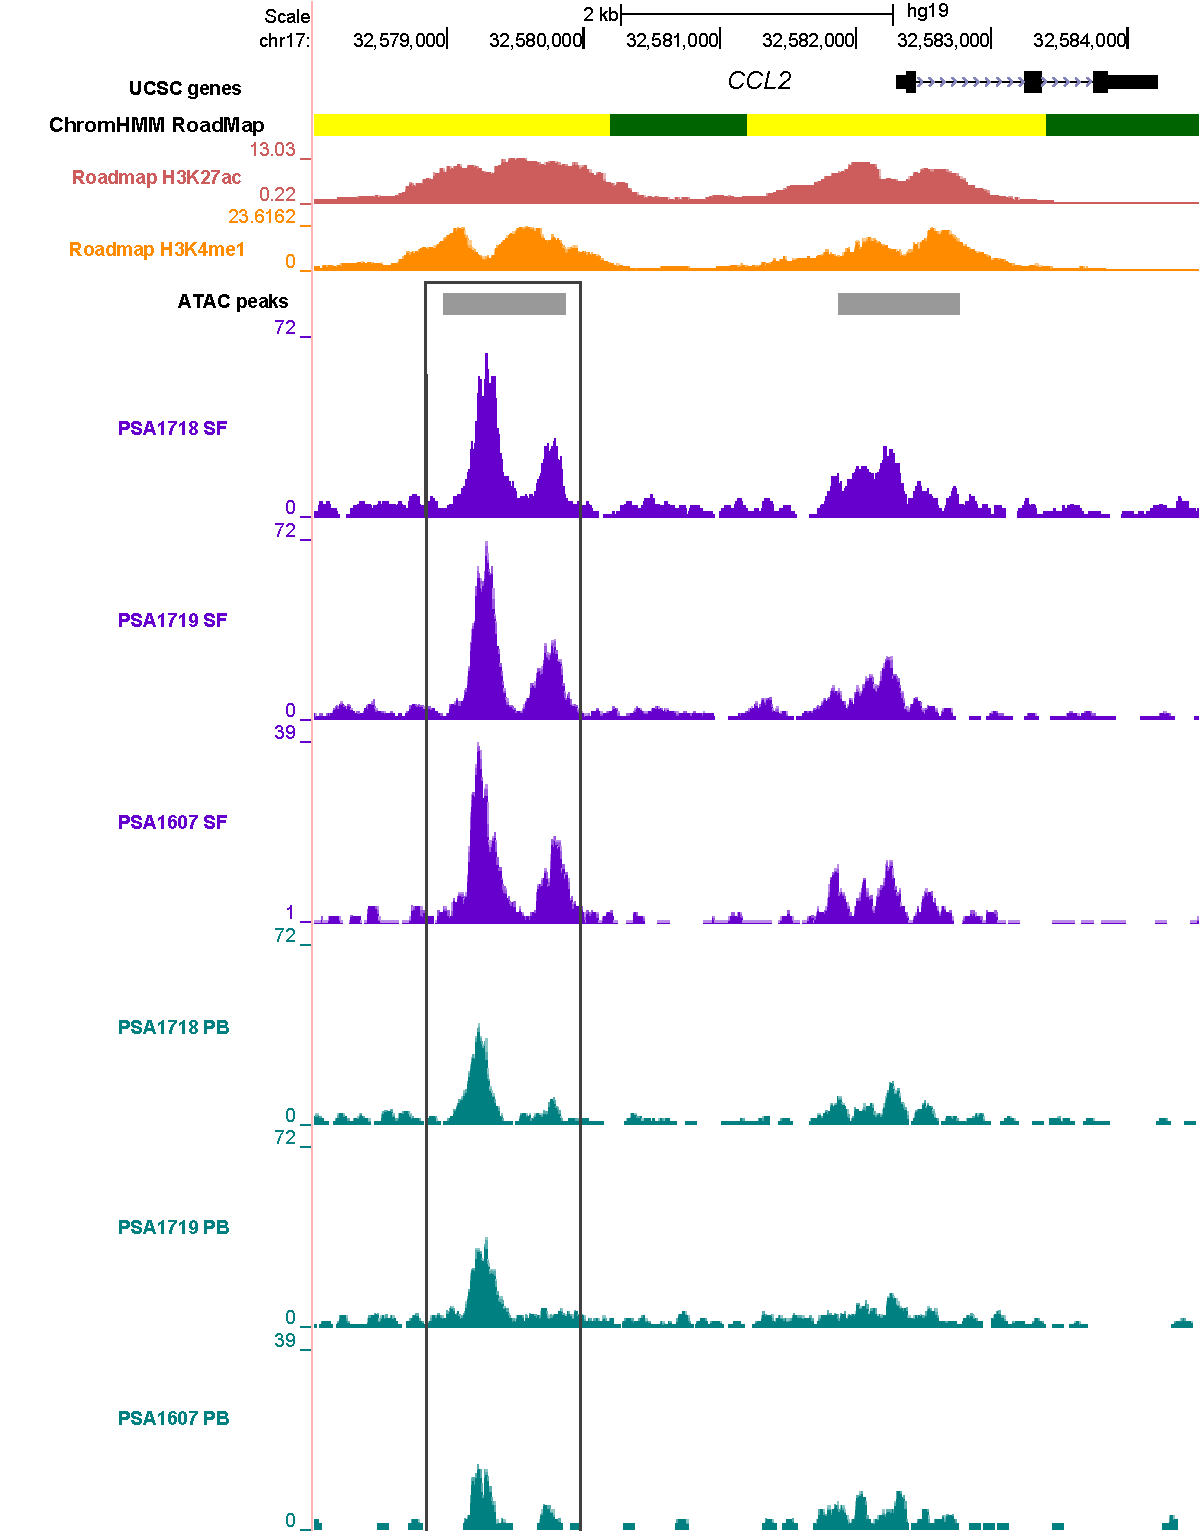
\includegraphics[width=\textwidth]{./Results3/pdfs/ATAC_PSA_CD14_UCSC_CCL2_track}%
\caption{}
\end{subfigure}%
~
\begin{subfigure}[b]{0.45\textwidth}
\centering 
\includegraphics[width=\textwidth]{./Results3/pdfs/ATAC_PSA_CD14_UCSC_CXCL10_promoter_and_upstream_5kb_track}%
\caption{}
\end{subfigure}
\caption[Chromatin landscape in CD14$^+$ monocytes in the proximity to \textit{CCL2} and \textit{CXCL10}.]{\textbf{Chromatin landscape in CD14$^+$ monocytes in the proximity to \textit{CCL2} and \textit{CXCL10}.} UCSC Genome Browser view illustrating the normalised ATAC read density (y-axis) for (A) a DAR located upstream \textit{CCL2} gene  and (B) two DARs at the promoter and upstream the \textit{CXCL10} gene (x-axis) in synovial fluid and peripheral blood CD14$^+$ monocytes from three PsA patients. In (A) and (B) DARs (black rectangles) were significant for FDR$<$0.01 and fold change$>$1.5 and showed presenting greater accessibility in synovial fluid when compared to peripheral blood. Tracks are colour-coded by tissue (SF=purple and PB=turquoise). Additional epigenetic tracks including chromatin segmentation maps and H3Kme1 and H3K27ac histone modifications from CD14$^+$ monocytes of the Roadmap Epigenomics Project are included.}
\label{figure:PsA_10X_qPCR_ATAC_CD14_CCL2_CXCL10}
\end{figure}


The DAR proximal to \textit{CCL2} was annotated as an enhancer according to Roadmap Epigenomics Project chromatin segmentation maps and overlaps an eRNA reported by FANTOM5 in CD14$^+$ monocytes. The DAR upstream \textit{CXCL10} co-localised with H3K4me1 and H3K27ac, reinforcing the enhancer properties of this region. In addition to the up-regulated transcriptional and protein expression in PsA CD14$^+$ monocytes, enzyme-linked immunosorbent assay (ELISA) quantification of MCP-1 and IP-10 levels conducted by collaborators revealed increased concentration of both chemokines in synovial fluid supernatant compared to plasma in the same ten PsA patients (Figure \ref{figure:CyTOF_cytokines_validation_cohort}E). This further supported the observed differences between synovial fluid and peripheral blood in chromatin accessibility, transcription and protein expression for \textit{CCL2} and \textit{CXCL10}.


%The expression of \textit{CCL2} was shown to be significantly up-regulated (p-value$<$0.05 and mean fold change$>$1.5) between synovial fluid and peripheral blood by qPCR only in CD14$^+$ monocytes only and was also identified by scRNA-seq as one of the up-regulated genes in the CC-mixed cluster (Figure \ref{figure:PsA_scRNAseq_vulcano_plots_mixed_and_IL7R_clusters}A and \ref{figure:PsA_scRNAseq_qPCR_ATAC_correlation}A and B). \textit{CXCL10} was also only significantly up-regulated CD14$^+$ monocytes between synovial fluid and peripheral blood from PsA patients by qPCR but no significant changes were found in the scRNA-seq differential analysis.Enzyme-linked immunosorbent assay (ELISA) quantification of MCP-1 and IP-10 levels conducted by collaborators revealed increased concentration of both chemokines in synovial fluid supernatant compared to plasma in the same 10 PsA patients (Figures \ref{figure:ELISA_SF_PsA} and \ref{figure:ELISA_SF_PsA}). This further supported the observed differences between synovial fluid and peripheral blood at the chromatin and transcriptomic levels for \textit{CCL2} and \textit{CXCL10}. %Overall, in the context of the data here presented suggests a tissue and cell type specific dysregulation of \textit{CCL2} expression in CD14$^+$ monocytes that may be related to alterations in the chromatin accessibility at an enhancer in the proximity to this gene.



\subsection{Prioritisation and interpretation of PsA GWAS SNPs}


\subsubsection{Bayesian fine-mapping using genotyping data}

Baysian fine-mapping for the PsA Immunochip GWAS signals identified by Bowes and colleagues \parencite{Bowes2015} was conducted using genotyping data from 1,103 patients and 8,900 controls. These samples only included the UK cohort from Bowes \textit{et al.}, 2015 PsA Immunochip. Bowes and colleagues also performed fine-mapping for a number of the loci with genome-wide or nominal evidence of association, reporting the number of independent signals as well as the number of SNPs in the 99\% credible set (SNPs accounting for 99\% of the association in a particular locus) but not the identity of each of those SNPs. Thus \textit{de novo} fine-mapping was conducted here to obtain the identity and the location of the SNPs in each credible set. % and perform integration with the chromatin accessibility data generated in the 4 immune cell types isolated from PsA patients samples and the DARs identified between synovial fluid and peripheral blood.

Fine-mapping was performed in 36 loci reported in Bowes \textit{et al.}, all showing at least nominal significance in their GWAS study. Out of the 36 loci, 22 showed log$_{10}$ABF$<$3 (cut-off used in Bunt \textit{et al.}, 2015) for the lead SNP in the fine-mapping association analysis (Table \ref{tab:PsA_loci_no_fine_mapping}). The majority corresponded to those signals with lowest significance in the GWAS association analysis (p-value$<10^{-4}$, e.g \textit{RSPH3/TAGAP} and \textit{ELMO1}) (Table \ref{tab:PsA_loci_no_fine_mapping}). Fine-mapping for GWAS signals with greater statistical significance (p-value$<10^{-4}$), for example \textit{DDX58}, also failed and were likely discarded by Bowes and colleagues fine-mapping based on the marker density in the region being lower than 100 SNPs. 
 

\begin{landscape}
\begin{center}
%\begin{longtable}[ht]{p{.25\textheight} p{.40\textheight} p{.25\textheight} p{.60\textheight}}
\renewcommand{\arraystretch}{0.8}
\begin{longtable}[htbp]{c c c c c c c c c c}
\caption[Summary table of the PsA GWAS loci presenting log$_{10}$BF$\geq$3 for the fine-mapping lead SNP.]{\textbf{Summary table of the PsA GWAS loci presenting log$_{10}$BF$\geq$3 for the fine-mapping lead SNP.} For 12 PsA loci log${_10}$BF of the fine-mapping lead SNP was 3 or greater. In 5 of those loci ($^{\ast}$) the fine-mapping lead SNP was in low LD (r$^{2}<$0.5) with the PsA GWAS SNP and/or did not contain it in the credible set. The effect size (OR) is reported relative to minor allele. FM=fine-mapping; MAF= minor allele frequency; OR=odds ratio; BF=Bayes factor; PP=posterior probability.}
\label{tab:PsA_fine_mapping_summary} \\
\toprule
\textbf{chr} & \textbf{Closest} & \textbf{FM} & \textbf{MAF} & \textbf{OR} & \textbf{log$_{10}$BF} & \textbf{PP} & \textbf{90\% credible} &\textbf{Bowes FM} & \textbf{Bowes 90\%}\\
    & \textbf{gene} & \textbf{lead SNP} & \textbf{cases/controls} & \textbf{FM} & \textbf{FM lead SNP} &  & \textbf{set} &\textbf{lead SNP} & \textbf{credible set} \\
\midrule
\midrule
2	 &\textit{IFIH1}	       & rs13406089$^{\ast}$	&0.28/0.33	&0.78	&4.58	&0.48	&2	&rs35667974	&4 \\
5	 &\textit{IL12B/ADRA1B}  & rs2546890 	          &0.42/0.48	&0.76	&6.53	&0.6	&23	&rs4921482	&3 \\
5	 &\textit{IL13}	         &rs2069616$^{\ast}$	  &0.5/0.44	  &1.25	&5.16	&0.05	&55	&NA	 &NA \\
1	 &\textit{IL23R}	       &rs12044149	          &0.32/0.25	&1.41	&9.83	&0.14	&29	&rs12044149	&34 \\
1	 &\textit{IL28RA/GRHL3}  &rs2135755$^{\ast}$	  &0.45/0.50	&1.20	&3.06	&0.03	&49	&NA	&NA \\
19 &\textit{ILF3}	         &rs11085727$^{\ast}$	  &0.25/0.30	&0.79	&3.83	&0.22	&35	&NA	&NA \\
17 &\textit{PTRF/STAT3}    &rs730086$^{\ast}$     &0.29/0.34 &0.81 &3.39 &0.39 &400	&NA	&NA \\
1	 & \textit{RUNX3}	       & rs6600250	          &0.45/0.50	&1.20	&3.07	&0.03	&48	&rs7523412	&52 \\
12 &\textit{STAT2/IL23A}	 &rs12368739	          &0.04/0.06	&1.70	&4.04	&0.02	&110 &	rs2020854	&121 \\
6	 & \textit{TRAF3IP2}	   &rs33980500	          &0.11/0.07	&1.71	&8.26	&0.87	&2	&rs33980500	&7 \\
19 &	\textit{TYK2}	       &rs11085727	          &0.25/0.30	&0.79	&3.83	&0.21	&32	&rs34725611	&5 \\
5	 & \textit{CSF2/P4HA2}	 &rs11242104            &0.48/0.43 &1.24 &5.31 &0.07 &58	&rs715285 &35 \\
%\medskip
\bottomrule
\end{longtable}
\end{center}
\end{landscape}


Amongst the loci that also failed to be fine-mapped in this thesis (log$_{10}$BF$<$3), 4 of them (\textit{B3GNT2}, \textit{NOS2A}, \textit{REL} and \textit{TNIP1}) had been successfully fine-mapped by Bowes and colleagues (Table \ref{tab:PsA_loci_no_fine_mapping}). This is likely due to the well established influence of sample size on the association analysis \parencite{Bunt2015}. %, highlighting the reduced power of the fine-mapping analysis presented here when compared to the one conducted by Bowes and colleagues due to the smaller sample size available (only UK cohort as previously mentioned).


Of the 12 loci passing the log$_{10}$BF$\geq$3 cut-off, 5 presented a fine-mapping lead SNPs in very low LD (r${^2}<0.5$) with the PsA GWAS lead SNP and/or did not contain the GWAS lead SNP in the credible set (Table \ref{tab:PsA_fine_mapping_summary} labelled with $^{\ast}$). This was the result of the association analysis identifying a different signal, in some cases the signal from a proximal locus, demonstrating the sensitivity of the association analysis for sample size. For example, the fine-mapping signal of the \textit{IL13} locus was confounded by the \textit{TYK2} signal, both in proximity at chr19. The additional 7 signals successfully fine-mapped in this study contained the GWAS lead SNP and also the fine-mapping lead SNPs from Bowes and colleagues analysis in their credible sets. For the 7 successfully fine-mapped loci, the size of credible sets ranged between 2 and 110 SNPs, with \textit{TRAF3IP2} being the only locus refined to fewer than 10 SNPs and showing log$_{10}$BF$>$5, generally considered the genome-wide significant cut-off (Table \ref{tab:PsA_fine_mapping_summary}). Furthermore, for \textit{IL23R} and \textit{TRAF3IP2}, the fine-mapping lead SNPs in this analysis was the same as the reported by Bowes and colleagues. In the step-wise conditional analysis a secondary independent signal was also identified for the \textit{IL12B/ADRAB1} locus; however the lead SNP in the analysis of this thesis (rs12653520) was different from the one reported by Bowes and colleagues (rs12188300). 




\subsubsection{Enrichment of fine-mapped SNPs with ATAC and eQTL data}

The 90\% credible sets of the 7 loci successfully fine-mapped in this analysis included a total of 292 unique SNPs. Overlapping epigenetic and expression data generated in clinical samples with the credible set of SNPs from PsA GWAS loci may be informative for refining putative functional causal variants in non-coding or intergenic GWAS associations compared to integrating epigenetic data from cell lines or healthy controls. Co-localisation of the genomic position of the credible set of SNPs with the significant differentially accessible regions (DARs with FDR$<$0.01 and fold change$>$1.5) identified between synovial fluid and peripheral blood in the four cell types did not reveal any overlap. Enrichment of fine-mapped SNPs in the proximity of DARs (10Kb window) was explored using as background sets of SNPs preserving the same LD structure, allele frequencies and distance to genes as the fine-mapped SNPs (detailed in Chapter \ref{ch:Mat}). Significant enrichment was only identified proximal to DARs in NK cells (Figure \ref{figure:PsA_FM_enrichment_analysis_ATAC}A) but not in the other three cell types (p-value$>$0.05). 

%\ToDo{Results of the enrichment in proximity 10Kb window when compared to common SNPs. Also should look if closer to DARs than the SNPs in r2 0.8 for each of the loci. That one for the viva}



\bigskip
\begin{figure}[htbp]
\centering
\begin{subfigure}[b]{0.40\textwidth}
\centering 
\includegraphics[width=\textwidth]{./Results3/pdfs/PsA_FM_enrichment_for_NK_DARs_ATAC_peaks_window}%
\caption{}
\end{subfigure}
~
\begin{subfigure}[b]{0.40\textwidth}
\centering 
\includegraphics[width=\textwidth]{./Results3/pdfs/PsA_FM_enrichment_for_CD14_consensus_ATAC_peaks_inside}%
\caption{}
\end{subfigure}%
~
\begin{subfigure}[b]{0.40\textwidth}
\centering 
\includegraphics[width=\textwidth]{./Results3/pdfs/PsA_FM_enrichment_for_CD4_consensus_ATAC_peaks_inside}
\caption{}
\end{subfigure}
~
\begin{subfigure}[b]{0.40\textwidth} 
%the [b] prevents offset in subcaptions
\centering
\includegraphics[width=\textwidth]{./Results3/pdfs/PsA_FM_enrichment_for_CD8_consensus_ATAC_peaks_inside}
\caption{}
\end{subfigure}%
~
\begin{subfigure}[b]{0.40\textwidth} 
%the [b] prevents offset in subcaptions
\centering
\includegraphics[width=\textwidth]{./Results3/pdfs/PsA_FM_enrichment_for_NK_consensus_ATAC_peaks_inside}
\caption{}
\end{subfigure}
\caption[Enrichment of PsA GWAS fine-mapped SNPs for DARs and ATAC peaks in CD14$^+$ monocytes, mCD4$^+$, mCD8$^+$ and NK cells.]{\textbf{Enrichment of PsA GWAS fine-mapped SNPs for DARs and ATAC peaks in CD14$^+$ monocytes, mCD4$^+$, mCD8$^+$ and NK cells.} (A) Histogram illustrating the percentage of SNPs from the 90\% credible set of the 7 successfully fine-mapped PsA loci overlapping a 10Kb window around DARs in NK cells (red line) compared to the same overlap found for each of the 1,000 sets of background SNPs. Histograms showing the percentage of the same fine-mapped SNPs overlapping ATAC peaks from the consensus list (red line) of (B) CD14$^+$ monocytes, (C) mCD4$^+$, (D) mCD8$^+$ and (E) NK cells vs the distribution of overlaps identified in each of the 1,000 sets of background SNPs. Significance of the enrichment is indicated as the p-value calculated using binomial test.}
\label{figure:PsA_FM_enrichment_analysis_ATAC}
\end{figure}


Additional overlap was performed between the 292 SNPs of the credible sets from the 7 successfully fine-mapped loci and the consensus list of ATAC peaks for each of the four cell types studied in this chapter (CP\_CD14, CP\_mCD4, CP\_mCD8 and CP\_NK). The largest number of overlaps between ATAC peaks and SNPs from the 90\% credible sets (17 SNPs) was found in CD14$^+$ monocytes, followed by mCD8$^+$, mCD4$^+$ and NK cells (Table \ref{tab:PSA_fine_mapping_ATAC_overlap}) with significant enrichment found in the four cell types when compared to matched backgrounds of SNPs (Figure \ref{figure:PsA_FM_enrichment_analysis_ATAC}B, C, D and E). %with increased significance when using 10Kb windows around the ATAC peaks (p-value$\leq$2.2x10$^{-16}$, histograms not included).
%The overlap of the fine-mapped SNPs with eQTL SNPs from GTEx and relevant immune cell types showed significant enrichment for a number of datasets when compared matched backgrounds of SNPs (Figure \ref{figure:PSA_fine_mapping_eQTL_enrichment}). Amongst the immune-related eQTL datasets, significant enrichment was only found for monocytes stimulated with LPS (2h or 24h) or IFN-$\gamma$. A number of GTEx eQTL datasets also showed significant enrichment, including whole blood and transformed fibroblasts, the last ones also being involved in the PsA structural changes \parencite{Espinoza1994}.


%\begin{figure}[htbp]
%\centering
%\includegraphics[width=0.7\textwidth]{./Results3/pdfs/PsA_FM_SNPs_overlap_eQTL_one_SNP_per_eGene}
%\caption[Association plot for the Bayesian fine-mapping results of the 5q31 (\textit{CSF2/P4HA2}) PsA GWAS signal.]{\textbf{Association plot for the Bayesian fine-mapping results of the 5q31 (\textit{CSF2/P4HA2}) PsA GWAS signal.} For each of the SNPs (dot) the location (x-axis) and the log$_{10}$BF (left y-axis) from the fine-mapping association analysis are shown. The colour of each dot indicated the LD relationship (r$^2$) with the lead SNP rs11242104 (in blue), being white=low LD (r$^{2}<$0.2), yellow=weak LD (r$^{2}<$0.5), orange=moderate LD (r$^{2}<$0.8) and red=high LD (r$^{2}$$\geq$0.8). The recombination rates in this window of the genome is indicated in the right y-axis (light blue line).}
%\label{figure:PSA_fine_mapping_eQTL_enrichment}
%\end{figure}



\begin{table}[htbp]
%\setlength{\tabcolsep}{20pt} only to stretch the columns if you want
%\renewcommand{\arraystretch}{1.5}
\centering
\begin{tabular}{@{} c c c}
\toprule
\textbf{ATAC cell type} & \textbf{90\% credible set}   &  \textbf{Cell-type specific}  \\
\textbf{master list}    & \textbf{overlapping SNPs}    &   \textbf{overlap of}   \\
									      &	\textbf{(number)}				     &   \textbf{fine-mapped SNPs} \\
\midrule
\midrule
 CD14$^+$ monocytes    & 32                            &  \textit{STAT2} (5), \textit{TYK2}(2)\\ 
                       &                               &  \textit{RUNX3}(1),\\
											 &                               &  \textit{TRAF3IP2}(1) \\
 mCD4$^+$              & 29                            &  \textit{CSF2}(1), \textit{IL23R}(1) \\
 mCD8$^+$              & 28                            &  \textit{RUNX3} (1)        \\
 NK                    & 19                            &  \textit{TYK2} (1)       \\
\bottomrule
\end{tabular}
\medskip %gap
\caption[PsA fine-mapped SNPs from the 90\% credible sets overlapping accessible chromatin identified by ATAC in four cell types.]{\textbf{PsA fine-mapped SNPs from the 90\% credible sets overlapping accessible chromatin identified by ATAC in four cell types.} The number of SNPs in the 90\% credible set union from each of the 7 fine-mapped loci overlapping ATAC peaks from each cell type consensus list are reported. The number of SNPs only found to overlap open chromatin in one cell type are indicated together with the locus in which the SNP was fine-mapped.}
\label{tab:PSA_fine_mapping_ATAC_overlap}
\end{table}


The 43 unique SNPs from the 90\% credible sets of the successfully fine-mapped regions within ATAC peaks were located across the \textit{CSF2} (8), \textit{IL12B} (3), \textit{IL23R} (4), \textit{RUNX3} (6), \textit{STAT2} (14), \textit{TRAF3IP2} (1) and \textit{TYK2} (7) loci. A number of these SNPs were found to only overlap accessible chromatin in one particular cell type. Interestingly, for the \textit{TRAF3IP2} locus, which was fine-mapped with the greatest resolution, none of the two SNPs of the 90\% credible set overlapped accessible chromatin in any of the four studied cell types.


%Notably, the GWAS Catalog SNPs overlapping ATAC accessible regions were significantly enriched (FDR$<$0.001) for particular terms from the Experimental Factor Ontology (EFO) (Figure \ref{figure:GWAS_traits_enriched_for_ATAC_ML}). The EFO is a hierarchical tree-like ontology where each term represents a (disease) trait or group of related (disease) traits with which disease-risk SNPs may be annotated (Figure \ref{figure:GWAS_traits_enriched_for_ATAC_ML}). Enrichment for general terms (towards the root of the tree) including autoimmune diseases, rheumatic diseases and skin diseases were found across all four cell types. Disease-specific terms (amongst the branches of the tree) related to these general terms, such as CD and IBD, were also found to be enriched for SNPs overlapping ATAC in all four cell types. Conversely, other "branches" from more general terms, including psoriasis and MS, presented significant enrichment (FDR$<$0.001) only in CD14$^+$ monocytes and mCD4$^+$ cells, respectively. Overall, this reinforced the specificity of the overlap between GWAS Catalog genetic variants not included in the fine-mapping credible set with accessible chromatin across the immune cell types investigated in this chapter.




%This enrichment of GWAS Catalogue SNPs overlapping mCD4$^+$ ATAC peks for MS is consistent with the key role of this cell type in the pathophysiology \parencite{Bielekova2000}.   



%\begin{figure}[htbp]
%\centering
%\includegraphics[width=0.75\textwidth]{./Results3/pdfs/Enrichment_for_FM_GWAS_cat_SNPs_overlapping_ATAC}
%\caption[Experimental Factor Ontology terms enriched in GWAS Catalog SNPs overlapping ATAC regions in four cell types.]{\textbf{Experimental Ontology Factor terms enriched for GWAS Catalog SNPs overlapping ATAC regions in four cell types.} Each term annotates a set of risk SNPs associated with a disease trait or a group of related disease traits. Enrichment analysis was performed using as input data the GWAS Catalog SNPs overlapping ATAC accessible chromatin regions. A minimum of ten SNPs overlap and FDR$<$0.001 was required for enrichment to be considered significant.}
%\label{figure:GWAS_traits_enriched_for_ATAC_ML}
%\end{figure}

\subsubsection{Integration of epigenetic and functional data at the \textit{RUNX3} locus}
Another of the successfully fine-mapped loci was \textit{RUNX3}, with the 90\% credible set containing 56 SNPs (Table \ref{tab:PsA_fine_mapping_summary} and Figure \ref{figure:RUNX3_chr5q31_fine_mapping_association_plot}). The integration with ATAC data from the four investigated cell types further narrowed down the number of putative causal variants to 6 SNPs. rs11249213 was one of the SNPs overlapping in CD14$^+$ monocytes, mCD4$^+$ and mCD8$^+$ cells a discrete consensus ATAC peaks annotated as an enhancer in the three cell types according to the corresponding chromatin segmentation maps. rs11249213 is located at an intergenic region, approximately 20Kb downstream the \textit{RUNX3} gene and 1Kb away from Bowes GWAS lead SNP rs7523412.  



\begin{figure}[htbp]
\centering
\begin{subfigure}[b]{0.5\textwidth}
\centering 
\includegraphics[width=\textwidth]{./Results3/pdfs/PSA_FM_Immunochip_RUNX3_association_plot}%
\caption{}
\end{subfigure}%
~
\begin{subfigure}[b]{0.5\textwidth}
\centering 
\includegraphics[width=\textwidth]{./Results3/pdfs/PSA_FM_Immunochip_5q31_association_plot}%
\caption{}
\end{subfigure}%
\caption[Association plot for the Bayesian fine-mapping results of the 5q31 (\textit{CSF2/P4HA2}) and \textit{RUNX3/SYF3} PsA GWAS signal.]{\textbf{Association plot for the Bayesian fine-mapping results of the 5q31 (\textit{CSF2/P4HA2}) and \textit{RUNX3/SYF3} PsA GWAS signal.} Association plots for the loci (A) 5q31 (\textit{CSF2/P4HA2}) and (B) \textit{RUNX3/SYF3}. For each of the SNPs (dot) the location (x-axis) and the log$_{10}$BF (left y-axis) from the fine-mapping association analysis are shown. The colour of each dot indicated the LD relationship (r$^2$) with the lead SNPs (blue diamond), being white=low LD (r$^{2}<$0.2), yellow=weak LD (r$^{2}<$0.5), orange=moderate LD (r$^{2}<$0.8) and red=high LD (r$^{2}$$\geq$0.8). The recombination rates in this window of the genome is indicated in the right y-axis (light blue line).}
\label{figure:RUNX3_chr5q31_fine_mapping_association_plot}
\end{figure}


In mCD8$^+$ the peak harbouring rs11249213 was identified as a DAR when using a threshold for significance of FDR$<$0.5, showing greater accessibility in synovial fluid when compared to peripheral blood (fold change=1.7) (Figure \ref{figure:RUNX3_fine_mapping_SNPs_epigenetic_track} black box). In mCD4$^+$ the same ATAC peak was only found in cells from synovial fluid only in two of the patients (PsA1618 and PsA1619). In contrast, in CD14$^+$ monocytes all 3 PsA patients showed accessible chromatin at the location of the SNP in both tissues. No significant eQTL signal was found for rs11249213 in immune-relevant cell types, including unstimulated CD4$^+$ and CD8$^+$ cells or unstimulated and treated monocytes (LPS or IFN-$\gamma$). None of the additional 5 SNPs of the credible set that overlapped ATAC peaks in at least one of the four cell types showed significant eQTL effect for any gene in in immune-related or GTEx datasets. Altogether, the observations based on in-house ATAC data may suggest a role of rs11249213 in regulating chromatin accessibility in the context of synovial inflammation only in mCD8$^+$ and mCD4$^+$ T cells.

\begin{figure}[htbp]
\centering
\includegraphics[width=0.7\textwidth]{./Results3/pdfs/PsA_fine_mapping_RUNX3_track}
\caption[Epigenetic landscape at the genomic location of the fine-mapped SNP rs11249213 at the \textit{RUNX3} PsA GWAS signal.]{\textbf{Epigenetic landscape at the genomic location of the fine-mapped SNP rs11249213 at the \textit{RUNX3} PsA GWAS signal.} UCSC visualisation of the epigenetic landscape at rs11249213 (red), within a mCD8$^+$ DAR (black box) when using a significance threshold of FDR$<$0.05. The track includes publicly available data for (A) ENCODE cluster for TF binding, (B) chromatin segmentation maps, (C) H3K4me1 (relative fold-enrichment) and in-house ATAC tracks (normalised counts) from 3 PsA patients for (D) CD14$^+$ monocytes, (E) mCD4$^+$, (F) mCD8$^+$ and (G) NK cells isolated from synovial fluid and peripheral blood.}
\label{figure:RUNX3_fine_mapping_SNPs_epigenetic_track}
\end{figure}



\subsubsection{Integration of epigenetic and functional data at 5q31 PsA-specific locus}
Fine-mapping was successfully performed for the 5q31 locus nearby \textit{CSF2/P4HA2} genes (Figure \ref{figure:RUNX3_chr5q31_fine_mapping_association_plot}), the only PsA-specific GWAS association identified in the Immunochip GWAS study from Bowes and colleagues \parencite{Bowes2015}. The fine-mapping conducted here revealed rs11242104 as the lead SNP for this locus (Table \ref{tab:PsA_fine_mapping_summary}, log$_{10}$BF=5.31 and PP=0.07), differing from the fine-mapping lead SNP reported by Bowes and colleagues, likely due to the differences in the sample size.



Integration of the in-house chromatin accessibility data with the 58 SNPs in the 90\% credible set showed only 8 variants overlapping ATAC peaks in at least one of the four cell types analysed in this chapter (Table \ref{tab:5q31_SNPs_ATAC_eQTL} and Figure \ref{figure:5q31_fine_mapping_SNPs_epigenetic_track} top panel). Either the lead SNP of this analysis or the one from Bowes and colleagues fine mapping overlapped ATAC peaks. Three of the variants highlighted by Bowes and colleagues as functionally relevant based on ENCODE data (rs10065787, rs27437 and rs7721882) were within an ATAC peak of at least one of the cell types isolated from PsA samples (Table \ref{tab:5q31_SNPs_ATAC_eQTL}). 


\begin{table}[htbp]
%\setlength{\tabcolsep}{20pt} only to stretch the columns if you want
\renewcommand{\arraystretch}{0.8}\text
\centering
\begin{tabular}{@{} c c c c}
\toprule
\textbf{SNP} & \textbf{Cell type ATAC}   & \textbf{Top eGene} & \textbf{Cell type } \\
             & \textbf{overlap}          &                    &\textbf{(adj p-value)}  \\
\midrule
\midrule
rs10065787   & CD14$^+$, mCD4$^+$        & \textit{P4HA2}   & CD14$^+$ LPS2 (2.4x10$^{-15}$),\\
             &                           &                  & CD14$^+$ LPS24 (5.9x10$^{-23}$) \\
						 &                           &                  & CD14$^+$ IFN-$\gamma$ (4.1x10$^{-20}$) \\
             &                           & \textit{SLC22A5} & CD14$^+$ UT (9.3x10$^{-33}$) \\
						 &                           &                  & CD14$^+$ IFN-$\gamma$ (6.6x10$^{-26}$)\\
						 &                           &                  & CD4$^+$ (1.6x10$^{-3}$) \\
						 &                           &                  & CD8$^+$ (8.0x10$^{-3}$) \\
						 &                           & \textit{SLC22A4} & CD14$^+$ UT (2.3x10$^{-11}$) \\
\midrule
rs11242104   & All                       &     NA        \\ 
\midrule
rs11242105   & All                       &     NA   \\
\midrule
rs2069803    & All                       & \textit{SLC22A5} & CD4$^+$ ($<$2.2x10$^{-308}$) \\
             &                           &                  & CD8$^+$ (4.5x10$^{-4}$) \\ 
\midrule
rs27437      & CD14$^+$, mCD4$^+$        & \textit{SLC22A5} & CD4$^+$ (1.9x10$^{-3}$)\\
             &                           &                  & CD8$^+$ (2.6x10$^{-2}$) \\ 
\midrule
rs4705908    & All                       & \textit{SLC22A5} & CD4$^+$ ($<$2.2x10$^{-308}$) \\
             &                           &                  & CD8$^+$ (8.7x10$^{-4}$)  \\
\midrule
rs2089855    & All                       & \textit{P4HA2}   & CD14$^+$ LPS2 (3.5x10$^{-25}$)\\
             &                           &                  & CD14$^+$ LPS24 (1.1x10$^{-34}$) \\
						 &                           &                  & CD14$^+$ IFN-$\gamma$ (3.1x10$^{-34}$) \\
             &                           & \textit{SLC22A5} & CD14$^+$ UT (8.8x10$^{-51}$) \\
						 &                           &                  & CD14$^+$ IFN-$\gamma$ (4.1x10$^{-36}$)\\
						 &                           &                  & CD4$^+$ ($<$2.2x10$^{-308}$) \\
						 &                           &                  & CD8$^+$ ($<$2.2x10$^{-308}$)  \\
\midrule
rs7721882    & mCD4$^+$                  & \textit{SLC22A5} & CD4$^+$ ($<$2.2x10$^{-308}$) \\
             &                           &                  & CD8$^+$ (1.5x10$^{-4}$) \\							
\bottomrule
\end{tabular}
\medskip %gap
\caption[Publicly available \textit{cis}-eQTL datasets reporting an effect for the PsA 5q31 GWAS locus fine-mapped SNPs (90\% credible set) overlapping ATAC accessible regions.]{\textbf{Publicly available and unpublished \textit{cis}-eQTL datasets reporting an effect for the PsA 5q31 GWAS locus fine-mapped SNPs (90\% credible set) overlapping ATAC accessible regions.} For each of the SNPs, the cell type for the ATAC overlap, the gene which expression is reported to be regulated by the SNP (eGene) and the cell type where the eQTL study was conducted are specified. The eQTLs datasets included in the analysis were CD14$^+$ monocytes (UT, LPS 2h, LPS 24h, IFN-$\gamma$) \parencite{Fairfax2014}, B cells \parencite{Fairfax2012}, total CD4$^+$ and total CD8$^+$ \parencite{Kasela2017}. adj p-value refers to the corrected p-value for multiple testing reported by each of the studies.} %neutrophils untreated \parencite{Naranbhai2015}, NK untreated (unpublished), }
\label{tab:5q31_SNPs_ATAC_eQTL}
\end{table}


Two relevant SNPs from the 90\% credible set in this analysis were rs2069803 and rs4705908, both overlapping ATAC peaks in all four cell types (Figure \ref{figure:5q31_fine_mapping_SNPs_epigenetic_track} panel 1 black and brown lines, respectively). Moreover, both SNPs also overlapped enriched regions for H3Kme1 from the Roadmap Epigenomics Project for some of the same cell types (Figures \ref{figure:5q31_fine_mapping_SNPs_epigenetic_track} panel 1, B and D) and rs2069803 was within a region annotated as enhancer in mCD4$^+$, mCD8$^+$ and NK cells, according to chromatin segmentation maps (Figure \ref{figure:5q31_fine_mapping_SNPs_epigenetic_track} panel 1, C). Although both SNPs overlapped accessible chromatin in all four cell types, the most significant \textit{cis}-eQTL signals were found for regulation of \textit{SLC22A5} expression in CD4$^+$ or CD8$^+$ T cells (Table \ref{tab:5q31_SNPs_ATAC_eQTL}), in line with Bowes and colleagues finding in their pilot eQTL study). Promoter capture Hi-C data in na\"{i}ve and total CD4$^+$ CD8$^+$ cells revealed interaction of the \textit{IL3} promoter bait containing rs2069803 with the promoter of \textit{SLC22A5}.

%rs4705908 also overlapped an enriched region fro H3K4me1 from the Roadmap Epigenomic Project, particularly in mCD4$^+$ and NK cells, and mapped to a CTCF binding site reported in GM12878 and LCLs cell lines (Figure \ref{figure:5q31_fine_mapping_SNPs_epigenetic_track} panel 1, B and D). Likewise, rs2069803 was located at a moderate H3K4me1 signal in mCD4$^+$, mCD8$^+$ and NK cells (Figure \ref{figure:5q31_fine_mapping_SNPs_epigenetic_track} panel 1 B) and within a region annotated as enhancer in mCD4$^+$, mCD8$^+$ and NK cells, according to chromatin segmentation maps (Figure \ref{figure:5q31_fine_mapping_SNPs_epigenetic_track} panel 1, C). Although rs2069803 and rs4705908 overlapped accessible chromatin in all 4 cell types, extremely significant \textit{cis}-eQTL signals regulating \textit{SLC22A5}, same eGene reported by Bowes and colleagues in their pilot eQTL study, were only found in CD4$^+$ or CD8$^+$ T cells for both SNPs (Table \ref{tab:5q31_SNPs_ATAC_eQTL}). Promoter capture Hi-C data in na\'{i}ve and total CD4$^+$ CD8$^+$ cells revealed interaction of the \textit{IL3} promoter bait containing rs2069803 with the promoter of \textit{SLC22A5}. %Interestingly, rs4705908 also appeared within the bait of the \textit{ACSL6} promoter interacting with the \textit{IL3} promoter bait, which also includes the previously mentioned rs2069803 variant. 



\begin{figure}[htbp]
\centering
\includegraphics[width=0.8\textwidth]{./Results3/pdfs/UCSC_chr5q31_credible_set_all_cell_types_multipanel_final}
\caption[Epigenetic landscape at the genomic location of fine-mapped SNPs for the 5q31 PsA GWAS signal.]{\textbf{Epigenetic landscape at the genomic location of fine-mapped SNPs for the 5q31 PsA GWAS signal.} (A) Location of the 6 SNPs from the 5q31 locus 90\% credible set overlapping ATAC peaks from the consensus list of at least one of the four cell types (blue). Relevant SNPs Bowes \textit{et al.} study, including the GWAS lead SNP (red), eQTL SNP showing the best correlation with the GWAS lead SNP (green) and one credible set SNP overlapping several ENCODE annotation features but not PsA ATAC data (purple). UCSC visualisation of the epigenetic landscape for rs4705908 (brown) and rs2069803 (black) in panel (1) and rs1006587 (red) and rs27437 (green) panel (2) representing 4 relevant fine-mapped SNPs overlapping PsA ATAC peaks and eQTLs signals. Also shown are publicly available data for (B) ENCODE cluster for TF binding, (C) chromatin segmentation maps, (D) H3K4me1 (relative fold-enrichment), (E) digital footprint and in-house ATAC tracks (normalised counts) from 3 PsA patients for (F) CD14$^+$ monocytes, (G) mCD4$^+$, (H) mCD8$^+$ and (I) NK cells isolated from synovial fluid and peripheral blood. The yellow box highlights a DAR found in CD14$^+$ monocytes near rs2069803 and rs4705908.}
\label{figure:5q31_fine_mapping_SNPs_epigenetic_track}
\end{figure}


rs2089855 was another of the fine-mapped SNPs overlapping ATAC in cell types showing extremely significant eQTL effect in regulating \textit{SLC22A5} expression in CD4$^+$ and CD8$^+$ cells (Table \ref{tab:5q31_SNPs_ATAC_eQTL}). This SNP is proximal to rs11955347, reported by Bowes \textit{et al.} as the most significant SNP correlating with expression of \textit{SLC22A5} in CD4$^+$ and CD8$^+$ in a pilot study (Figure \ref{figure:5q31_fine_mapping_SNPs_epigenetic_track}A in green). rs2089855 and rs11955347 were also \textit{cis}-eQTL SNPs for \textit{SLC22A5} and \textit{P4HA2} expression in unstimulated and stimulated monocytes (LPS or IFN-$\gamma$), respectively (Table \ref{tab:5q31_SNPs_ATAC_eQTL}). Similarly, rs10065787 mapped to an ATAC peak in CD14$^+$ monocytes and mCD4$^+$ cells with moderate enrichment for the enhancer histone mark H3K4me1 in mCD4$^+$ (Figure \ref{figure:5q31_fine_mapping_SNPs_epigenetic_track} panel 2 red line, D, F, and G) and showed an eQTL effect for \textit{SLC22A5} and \textit{P4HA2} expression in unstimulated and stimulated monocytes (LPS2, LPS24, IFN-$\gamma$), respectively (Table \ref{tab:5q31_SNPs_ATAC_eQTL}). Chromatin conformation data using promoter capture HiC \parencite{Javierre2016} in unstimulated monocytes does not clearly reveal interaction for rs10065787 with the promoter of \textit{P4HA2}, which may be only found under stimulation.

%rs10065787, highlighted by Bowes \textit{et al.} for overlapping with ENCODE clusters of occupancy for TFs relevant in CD4$^+$ and CD8$^+$ biology, was . Chromatin conformation data using promoter capture-HiC \parencite{Javierre2016} in unstimulated monocytes does not clearly reveal interaction for rs10065787 with the promoter of \textit{P4HA2}, which may be only found under stimulation.


Altogether, the integration of in-house and publicly available epigenetic and functional data with the SNPs from the 90\% credible set obtained by fine-mapping suggests a role for the 5q31 PsA-specific GWAS association in regulating expression of \textit{P4HA2} and \textit{SLC22A5}, not only in T cells but also in monocytes under different pro-inflammatory conditions.





%%%%%%%%%%%%%%%%%%%%%%%%%%%%%%%%%%%%%

%Promoter capture-HiC from Javierre \textit{et al.} in tCD4$^+$ and tCD8$^+$ cells revealed  direct rs743564 interaction with \textit{P4HA2} and proximity to a downstream fragment that presents frequent interaction with \textit{SLC22A5} promoter in both cell types. Interestingly, rs1469149, another SNP from the credible overlapping a mCD4$^+$-specific ATAC peak (Table \ref{tab:5q31_SNPs_ATAC_eQTL}) is found to be in the same bait as rs743564 interacting with \textit{SLC22A5} promoter. The SNP rs1469149 also presents a extremely significant signal for a tCD4$^+$ eQTL regulating \textit{SLC22A5} expression and less significant eQTLs in stimulated monocytes (Table \ref{tab:5q31_SNPs_ATAC_eQTL}). 


%In contrast, rs10065787 was found to be a \textit{cis}-eQTL in stimulated monocytes (LPS 2h, LPS 24h and IFN-$\gamma$) regulating \textit{P4HA2} expression (Table \ref{tab:5q31_SNPs_ATAC_eQTL}). The nearby SNP rs27437 overlapped an ATAC peak in CD14$^+$ monocytes and mCD4$^+$ and the same TFBS site cluster than rs10065787 (Table \ref{tab:5q31_SNPs_ATAC_eQTL} and Figure \ref{figure:5q31_fine_mapping_SNPs_epigenetic_track} right hand side panel green line). The enhancer histone mark H3K4me1 was absent in CD14$^+$ monocytes and only moderate in mCD4$^+$ (Figure \ref{figure:5q31_fine_mapping_SNPs_epigenetic_track} right hand side panel). Interestingly, \textit{cis}-eQTL were only reported for tCD4$^+$ and tCD8$^+$ associated to modulation of expression for \textit{SLC22A5}, the same eGene reported by Bowes and colleagues in their pilot eQTL study. Nevertheless, chromatin conformation data has not revealed any interaction for rs10065787 with the promoter of \textit{P4HA2}. Conversely, rs27437 is relatively close to the bait in \textit{IL3} which interacts with \textit{SLC22A5}, potentially bringing this SNP in proximity with the promoter of the eQTL eGene repoted in tCD4$^+$ and tCD8$^+$ Kasela's dataset. 
%
%Another two relevant SNPs from the 90\% credible set here reported were rs2069803 and rs4705908, both overlapping ATAC peaks in all four cell types (Figure \ref{figure:5q31_fine_mapping_SNPs_epigenetic_track} left hand side panel black and brown lines, respectively). Rs4705908 is located upstream the promoter of \textit{ACSL6} gene and is overlapping a region enriched for H3K4me1, supporting a regulatory role for that region. Notably, rs4705908 is mapping to a CTCF binding site reported in GM12878 and LCLs cell lines. Likewise, rs2069803 is also overlapping open chromatin and moderate H3K4me1 signal in mCD4$^+$, mCD8$^+$ and NK cells (Figure \ref{figure:5q31_fine_mapping_SNPs_epigenetic_track} left hand side panel). The region has also been annotated as enhancer and weakly transcribed in mCD4$^+$, mCD8$^+$ and NK cells by the Epigenome Roadmap chromatin segmentation maps (yellow and light green in \ref{figure:5q31_fine_mapping_SNPs_epigenetic_track} left hand side panel). Although accessible chromatin has been identified at rs2069803 and rs4705908 for all cell types, \textit{cis}-eQTL for these two SNPs have only been reported in CD4$^+$ or CD8$^+$, with the genotypes of both SNPs correlating with regulation of \textit{SLC22A5} expression, with extremely high significance in tCD4$^+$ cells (Table \ref{tab:5q31_SNPs_ATAC_eQTL}). Promoter capture Hi-C data in na\'{i}ve and total CD4$^+$ CD8$^+$ cells revealed interaction of the \textit{IL3} promoter bait containing rs2069803  with the promoter of \textit{SLC22A5}. Interestingly, rs4705908 appeared also within the bait of the \textit{ACSL6} promoter interacting with the \textit{IL3} promoter bait, which also includes the rs2069803 as previously mentioned \parencite{Javierre2016}. Overall, promoter-capture HiC data revealed potential physical interaction between rs27437, rs2069803 and rs4705908 in CD4$^+$ and CD8$^8$ cells with potential functional relevance in gene expression regulation of \textit{SLC22A5}.

%The PsA GWAS lead SNP rs715285 was also contained in the credible set but was mapped to a region of closed chromatin and depleted signals for H3K4me1 and digital footprint in all four cell types. Likewise, the aforementioned eQTL SNP rs11955347 from Bowes study showing the strongest correlation with \textit{SLC22A5} expression also appeared in a region depleted for open chromatin and activating epigenetic marks, suggesting that one or more of the previously highlighted SNPs from the 90\% credible set may be responsible for the effect on gene expression regulation detected by eQTL studies for \textit{P4HA2} and \textit{SLC22A5} expression. 



%\subsubsection{Overview of fine-mapping and epigenetic data integration for other loci}
%In addition to the 5q31 locus (\textit{CSF2/P4HA2}), another seven loci were successfully fine-mapped in this analysis. As previously mentioned, integration of epigenetic data and fine-mapping credible set of SNPs is particularly relevant when trying to identify putative causal SNPs for GWAS signals lying in non-coding regions. An example amongst the fine-mapped loci is \textit{IL12B}, for which a PsA GWAS lead SNP as well as the fine-mapped lead SNP found in this analysis were located upstream of the gene. Out of the 52 SNPs identified in the 90\% credible set only four appeared to overlap accessible chromatin in at least two of the cell types analysed by ATAC in PsA samples and they were not in LD with common non-synonymous SNPs in \textit{IL12B}. The PsA GWAS SNP rs4921482 (primary signal in Bowes and colleagues) overlapped a strong ATAC peak in all cell types as well as H3K4me1 enhancer marks. However, none of the four SNPs in the credible set overlapping ATAC peaks was found within a \textit{cis}-eQTL signal in any of the explored datasets.
%
%
%For another two loci fine-mapped in this analysis, \textit{STAT2/IL23A} and \textit{TRAF3IP2}, previous evidence for high LD between the psoriasis GWAS signal and missense coding variants in \textit{STAT2} and \textit{TRAF3IP2}, respectively, had been reported \parencite{Tsoi2012}. For the psoriasis GWAS \textit{STAT2} signal, Tsoi \textit{et al.}, 2012 highlighted a missense mutation (rs2066807) with a predicted highly damaging effect in this gene that is in very high LD with the GWAS lead SNP (Figure \ref{figure:STAT2_fine_mapping_SNPs_epigenetic_track} purple line). This SNP also appeared in the 90\% credible set of SNPs in this analysis. Although rs2066807 did not overlap ATAC accessible chromatin in any of the four cell types, it mapped to a RUNX3 and CTCF binding site in the cell lines GM12878 and K562. SNPs from the credible set located in the vicinity of this missense variant were found within eQTL signals of interest. For example, rs2371494 overlapped an ATAC peak in all four cell types (Figure \ref{figure:STAT2_fine_mapping_SNPs_epigenetic_track} black line) and presented a highly significant eQTL effect for \textit{STAT2} expression in unstimulated monocytes (FDR=7.54x10$^{-31}$) and to a lesser significance under IFN-$\gamma$ stimulation (FDR=9.94x10$^{-6}$). Fairfax and colleagues reported a negative effect for the major allele (G) of rs2371494 and also for the PsA GWAS lead SNP rs2020854 (T) (LD r$^2$=0.79) in both conditions, indicating increased expression of \textit{STAT2} for the GWAS risk allele. Interestingly, the nearby SNP rs57870697 which is in very high LD (r${^2}\geq$0.79) with rs2371494, overlapped a CD14$^+$ monocyte specific ATAC peaks in synovial fluid and peripheral blood (Figure \ref{figure:STAT2_fine_mapping_SNPs_epigenetic_track} red line) but no eQTL for any gene has been reported at the location of this SNP.
%
%Lastly, fine-mapping for the \textit{RUNX3/SYF3} locus identified 48 SNPs in the credible set, of which six overlapped ATAC peaks in CD14$^+$ monocytes and mCD8$^+$ cells. One mapped to a discrete mCD8$^+$ specific peak at the edge of a CTCF and RELA binding site in GM12878. Nevertheless, no eQTL has been reported for any of the six SNPs overlapping ATAC in any of the datasets.



%%Fine-mapping of the PsA GWAS signal in chr2 nearby \textit{STAT2} and \textit{IL23A} genes yielded 110 SNPs in the credible set of SNPs, very similar to the size of the credible set reported by Bowes and colleagues for this locus. Out of the 110 SNPs, 8 were found to overlap with an ATAC peak in at least one cell type. Amongt those 8 SNPs, rs2371494 located upstream the \textit{IL23A} and \textit{STAT2} genes, appeared to be of particular interest. Rs2371494 overlapped an ATAC peak in all four cell types (Figure \ref{figure:STAT2_fine_mapping_SNPs_epigenetic_track} black line) and presented a highly significant eQTL effect for \textit{STAT2} expression in unstimulated monocytes (FDR=7.54x10${^-31}$) and to a lesser significance under IFN-$\gamma$ stimulation (FDR=9.94x10${^-6}$). Fairfax and colleagues reported a negative effect for the major allele (G) of rs2371494 and also for the PsA GWAS lead SNP rs2020854 (T) (LD r$^2$=0.79) in both conditions, indicating increased expression of \textit{STAT2} for the GWAS risk allele. Additional eQTLs with lower significance for other eGenes were also reported for rs2371494 and other SNPs in the credible set. 
%
%%Interestingly, rs35157967 and rs57870697, two SNPs of the credible set in the vicinity and in very high LD (r${^2}\geq$0.79) with rs2371494, were overlapping synovial fluid and peripheral blood CD14$^+$ monocyte specific ATAC peaks (Figure \ref{figure:STAT2_fine_mapping_SNPs_epigenetic_track} red and green lines). Rs35157967 is located upstream \textit{IL23A} and \textit{STAT2} genes and rs57870697 is found within a \textit{STAT2} intron. Both SNPs were also mapping to H3K4me1 in CD14$^+$ monocytes and ENCODE clusters for TFs. Notably, rs35157967 is overlapping binding sites for for STAT2 and IRF1 in K562 cell line. The fact that no eQTL for \textit{STAT2} gene has been reported for none of those two SNPs in the same conditions as for rs2371494 may be consequence of those two SNPs not having been imputed in Fairfax \textit{et al.} analysis. Hypothetical existence of an eQTL signal for \textit{STAT2} could suggest a functional role of rs35157967 and/or rs57870697 in the regulation of \textit{STAT2} expression in homeostasis and under IFN-$\gamma$ stimulation in CD14$^+$ monocytes. Nevertheless, the proximity of the SNPs in the credible set to coding SNPs
%
%%In terms of dysregulation of expression in the affected tissue, scRNA-seq analysis did not detect \textit{STAT2} or any of the proximal genes as differentially expressed between synovial fluid and peripheral blood in CD14$^+$ monocytes. Regarding the suitability of \textit{STAT2} as a psoriasis drug target, Pi showed high prioritisation for this gene as a putative drug target (position 70) in psoriasis.



% may be in LD with a coding variant?
%\begin{figure}[htbp]
%\centering
%\includegraphics[width=0.6\textwidth]{./Results3/pdfs/UCSC_STAT2_IL23A_credible_set_all_cell_types_all_epigenetic_marks}
%\caption[Epigenetic landscape at the genomic location of three fine-mapped SNPs from the \textit{STAT2/IL23A} PsA GWAS signal.]{\textbf{Epigenetic landscape at the genomic location of three fine-mapped SNPs from the \textit{STAT2/IL23A} PsA GWAS signal.} UCSC visulisation of the epigenetic landscape for three relevant fine-mapped SNPs at the \textit{STAT2/IL23A} locus (x-axis), including rs2371494 (black line), rs35157967 (red line) and the missense putative damaging mutation reported by Tsoi \textit{et al.}, 2012 rs2066807 (purple line). ATAC tracks from three PsA patients and four cell types isolated from synovial fluid (purple) and peripheral blood (turquoise) are included. Publicly available epigenetic data (H3Kme1, chromatin segmentation maps, digital footprint and ENCODE cluster for TF binding) generated in the same cell types as the in-house ATAC are also included. H3K4me1 relative fold-enrichment signal and ATAC normalised counts within each cell type are shown (y-axis).}
%\label{figure:STAT2_fine_mapping_SNPs_epigenetic_track}
%\end{figure}

 

%%%%%%%%%%%%%%%%%%%%%%%%%%%%%%%%%%%%%%%%%%%%%%%%%%
\section{Discussion}


\subsection{Characterising chromatin accessibility in PsA samples}


The epigenetic landscape of immune cells isolated from PsA patients peripheral blood and synovial fluid has been characterised and compared in this chapter, representing the first study of chromatin accessibility in this disease to date. The interrogated cell types (CD14$^+$ monocytes, mCD4$^+$, mCD8$^+$ and NK) are key players in the innate and adaptive immune responses dysregulated in PsA pathophysiology. In particular, expansion of mCD4$^+$ and mCD8$^+$ cells in the synovium of PsA patients has been previously reported, and GWAS have highlighted significant associations within or nearby T cell immune response genes \parencite{Taams2018}.

Differential chromatin accessibility analysis in this chapter showed that in all four cell types the majority of DARs were located at intergenic and intronic regions annotated as enhancers and showed enrichment for eRNAs identified in the FANTOM project \parencite{FANTOM2014}. Notably, CD14$^+$ monocytes showed the largest number of DARs between synovial fluid and peripheral blood, with 9.1\% of the interrogated ATAC regions being differentially accessible. Pathway enrichment analysis using genes proximal to DARs revealed differences between synovial fluid and peripheral blood in all four cell types. In synovial fluid, enrichment for the NF-$\kappa$B pathway was found in CD14$^+$ monocytes, consistent with the TNF-$\alpha$ signature and the efficacy of anti-TNF therapies in PsA \parencite{Mahil2016}. Interestingly, open chromatin in peripheral blood mCD8$^+$ T cells was enriched for Wnt signaling pathway, which is involved in many biological processes and its dysregulation is associated with a number of autoimmune diseases including RA \parencite{Miao2013}. In this data, the significantly increased chromatin accessibility near Wnt signalling genes in peripheral blood mCD8$^+$ cells may be related to an increased recall proliferation capacity of the circulating cells compared to the tissue-resident \parencite{Boudousquie2014}. In NK cells from peripheral blood increased chromatin accessibility was found at genes involved in NK-mediated cytotoxicity. NK CD56$^{bright}$ cells resident at sites of inflammation are more specialised in cytokine production than in cytotoxic response \parencite{Michel2016}. Notably, flow-cytometry data in these patients have shown a reduced proportion of CD56$^{bright}$ cells in peripheral blood compared to synovial fluid, which would be consistent with this enrichment of NK peripheral blood open DARs for genes involved in the cytotoxic response.

Overall, this approach has identified robust differences in chromatin accessibility between synovial fluid and peripheral blood in PsA patients, in line with similar studies conducted in other diseases \parencite{Scharer2016,Wang2018,Corces2016}. Although these findings suggest meaningful functional differences between circulating and affected tissue immune cells, a limitation of pathway analysis in ATAC is linking open chromatin to genes. Annotation of ATAC peaks to nearby genes has been extensively used in the literature \parencite{Scharer2016,Ackermann2016, Corces2016, Wang2018}; however, this approach fails to evaluate long range regulatory effects and assumes that accessible chromatin regulates neighbouring regions. %Moreover, accessible chromatin is not a definitive marker for regulatory regions and mapping of histone marks such as H3K4me1 and H3K27ac together with eRNA quantification will help to refine the functional relevance of the identified DARs.   
   

%\subsection{Biological insights in the integration of chromatin accessibility, gene expression and proteomics data in PsA}

\subsection{Bulk qPCR  expression profiling and integration with paired chromatin accessibility data}

Recent reports have investigated differences in the transcriptional profiles between PBMCs, bulk T cells, SFMCs and synovial tissue from PsA patients \parencite{Dolcino2015, Fiocco2015}, but a comparative analysis in matched discrete cell subpopulations from synovial fluid and peripheral blood of the same patient was lacking. The pilot study presented in this chapter has characterised the expression of relevant immune genes in CD14$^+$ monocytes, mCD4$^+$ and mCD8$^+$ cells isolated from synovial fluid and peripheral blood. 

In this study, CD14$^+$ monocytes and mCD8$^+$ showed the largest number of statistically significant DEGs between synovial fluid and peripheral blood. Integration of transcriptome profiling with paired ATAC data revealed that a small number of the DEGs between synovial fluid and peripheral blood were nearby DARs showing changes in the same direction. %This overlap only presented significant enrichment for CD14$^+$ monocytes. 

 
Pro-inflammatory genes, including \textit{TNFA}, \textit{CXCL13} or \textit{CCL18}, were found to be up-regulated in synovial fluid compared to peripheral blood in at least one cell type. These genes were previously reported by Dolcino and colleagues as DEGs in synovial membranes of PsA patients compared to controls \parencite{Dolcino2015}, suggesting the up-regulation of those genes to be a feature of PsA joints. Genes such as \textit{CXCL10}, \textit{CCL7}, and \textit{CCL17} were only up-regulated in CD14$^+$ monocytes, consistent with their role in the migration of monocytes from bone marrow to tissues \parencite{Tsou2007}. In contrast, genes involved in Th-17 cell response such as \textit{CXCL13} and \textit{IL26} \parencite{Takagi2008} only showed up-regulation in synovial fluid mCD4$^+$ and/or mCD8$^+$ when compared to peripheral blood. %, not changing expression between the two tissues in CD14$^+$ monocytes.

A preliminary analysis comparing DEGs between PsA patients and controls in peripheral blood with the genes differentially expressed between synovial fluid and peripheral blood in patients identified a number of systemic, tissue-specific and putative disease specific DEGs. In CD14$^+$ monocytes, a much larger number of immune-relevant genes were differentially expressed between the two tissues from patients than between PsA patients and healthy controls in peripheral blood. This is likely due to the plasticity of monocytes and their ability to differentiate into macrophages at the inflamed synovium \parencite{Yoon2014, Park2016}. A particularly interesting systemic DEG in mCD8$^+$ cells was \textit{CCR10}, a chemokine receptor co-expressed by a subset of memory cells that preferentially migrate to skin, which was also up-regulated in CD8$^+$ cells in the psoriasis cohort (Chapter \ref{ch:Results2}) and in patients with atopic dermatitis \parencite{Hijnen2005}. In mCD4$^+$, \textit{GPR68}, a G protein-coupled receptor (GPCR) was up-regulated in peripheral blood of PsA patients when compared to controls with further increased expression in synovial fluid. \textit{GPR68} undergoes activation through pH acidification, which is a characteristic feature of synovial tissue \parencite{Biniecka2016, Saxena2012}. Another member of the acid-sensing GPCR family, \textit{GPR65}, has been associated with other immune mediated diseases, including AS, CD and MS, and is a marker of pathogenic Th-17 cells \parencite{Cortes2013,Lassen2016,Wirasinha2018,Gaublomme2015, Al-Mossawi2017}. 

\textit{SPP1} and \textit{FN1} were the most significantly up-regulated genes in synovial fluid compared to peripheral blood of PsA patients, in line with previous findings \parencite{Dolcino2015} and interestingly no significant changes in peripheral blood between PsA patients and controls was observed. However, Dolcino and colleagues did detect a moderate up-regulation of \textit{SPP1} in peripheral blood in PsA patients. \textit{FN1} encodes fibronectin-1, a main component of the cartilage matrix, involved in cell adhesion, migration, growth and differentiation and found to be highly expressed in RA inflamed synovium \parencite{Chang2005}. \textit{FN1} has also shown to induce bone resorption mediated by pro-inflammatory mediators, such as nitric oxide and IL-1$\beta$ \parencite{Gramoun2010}. Notably, only in CD14$^+$ monocytes, two synovial fluid open DARs were found at the promoter and downstream of \textit{FN1}, consistent with the results from the differential expression analysis. 

Pathway analysis using significant qPCR DEGs between synovial fluid and peripheral blood revealed enrichment for chemokine, TLR and NOD-like signalling pathways in CD14$^+$ monocytes. This was consistent with the well-known role of TLR and NOD-like receptors in rheumatic diseases \parencite{McCormack2009}. %The significant up-regulation of the receptors \textit{TLR1} and \textit{TLR2} in synovial fluid CD14$^+$ monocytes compared to peripheral blood contributed to the enrichment of the TLR signaling pathway. Other studies have also reported increased \textit{TLR-2} and \textit{TLR-4} expression in SFMCs compared to PBMCs in patients with juvenile idiopathic arthritis \parencite{Myles2011}. 
NOD-like signalling has also been highlighted in the genome-wide trancriptomic analysis in lesional and uninvolved psoriatic skin presented in Chapter \ref{ch:Results2}. %The nicotinamide enzyme coded by \textit{NAMPT} was up-regulated in synovial fluid compared to peripheral blood and its expression by pro-inflammatory monocytes mediates the production of pro-inflammatory cytokines and Th-17 cell differentiation, showing potential as a drug target in an arthritis mouse model \parencite{Presumey2013.} 
Down-regulation of the TLR inhibitor \textit{SIGIRR}  \parencite{Ueno-Shuto2014} and up-regulation of \textit{TLR1}, \textit{TLR2}, \textit{MYD88} in the qPCR array may lead to increased activation of NF$\kappa$B TF in synovial fluid CD14$^+$ monocytes. This is consistent with significant reduction of NF-$\kappa$B activation upon etanercept treatment in PsA synovial biopsies \parencite{Lories2008}. The enrichment of synovial fluid open DARs in the proximity of genes within the NF-$\kappa$B pathway is consistent with the transcriptional up-regulation of downstream genes such as \textit{TNFA}, \textit{CCL2} and \textit{CCL5} and subsequent enrichment of chemokine signalling. In mCD4$^+$, enrichment of the IL-10 signalling pathway was interesting in the context of the expansion of Tregs in synovial fluid observed by flow cytometry analysis in the same samples. Tregs are characterised by the expression of anti-inflammatory cytokines, importantly IL-10 \parencite{Garra2004} and qPCR data showed a significant increase of the IL-10 receptor subunit $\alpha$ \textit{IL10RA} and a similar trend for \textit{IL10} in synovial fluid mCD4$^+$ and mCD8$^+$ compared to peripheral blood. This may suggest that inflammation in PsA is refractory to the immunomodulatory effects of IL-10 in synovial fluid or counterbalanced by its immunostimulatory properties, in line with failure of IL-10 agonist therapy in the treatment of CD and psoriasis \parencite{Marlow2013, Kimball2002}.


%The pilot study presented in this chapter has characterised the expression of relevant immune genes in CD14$^+$ monocytes, mCD4$^+$ and mCD8$^+$ cells isolated from synovial fluid and peripheral blood and integrated it with paired chromatin accessibility data from the same samples. In this study, CD14$^+$ monocytes and mCD8$^+$ presented the largest number of consistently differentially expressed genes between synovial fluid and peripheral blood. In the 3 cell types, \textit{SPP1} and \textit{FN1} were the most significantly dysregulated genes between synovial fluid and peripheral blood, in line with the finding from Dolcino and colleagues when comparing synovial membranes and peripheral blood from the same patients \parencite{Dolcino2015}. Other highly DEGs reported in Dolcino's study, including \textit{TNFA}, \textit{CXCL13} or \textit{CCL18}, were also found to be dysregulated between synovial fluid and peripheral blood in at least one of the cell types. Genes such as \textit{CXCL13} and \textit{IL26} appeared significantly up-regulated in synovial fluid mCD4$^+$ and/or mCD8$^+$ when compared to peripheral blood but did not show differential expression in CD14$^+$ monocytes, consistent with their role in Th17 cell biology \parencite{Takagi2008}. The integration of differences in peripheral blood gene expression between PsA patients and controls with the cross-tissue comparison within patients led to identification of systemic, tissue-specific and putative-disease specific modulated genes in this pilot data. According to my data,  more profound transcriptional changes across PsA tissues (tissue-specific genes) were identified when compared to changes in expression between PsA patients and controls in peripheral blood for CD14$^+$ monocytes and mCD8$^+$ cells. Systemic genes for mCD8$^+$ cells included for example \textit{CCR10}, a chemokine receptor co-expressed by a subset of memory cells that preferentially migrate to skin, which has also been identified as an up-regulated gene in tCD8$^+$ cells in the psoriasis cohort (Chapter \ref{ch:Results2} and in patients with atopic dermatitis \parencite{Hijnen2005}. Interestingly, \textit{SPP1} and \textit{FN1} appeared in the tissue-specific category in the three cell types. Dolcino and colleagues had reported these genes as the two most dysregulated when comparing bulk synovial membrane transcriptome from PsA patients and healthy individuals \parencite{Dolcino2015}. My data suggests that CD14$^+$ monocytes, mCD4$^+$ and mCD8$^+$ cells may all contribute to the up-regulation of \textit{SPP1} and \textit{FN1} in the PsA synovium membranes. The \textit{SPP1} protein product, osteopontin, is a cytokine and chemokine expressed by many cell types, including monocytes/macrophages and T cells. It is involved in cell migration, adhesion and cell-mediated immune response through regulation of T cells, importantly in Th-17 \parencite{Morimoto2010}. \textit{SPP1} also plays a role in other chronic inflammatory and autoimmune diseases \parencite{Rittling2015}. \textit{FN1} encodes fibronectin-1, a main component of the cartilage matrix, involved in cell adhesion, migration, growth and differentiation and found to be highly expressed in RA inflamed synovium \parencite{Chang2005}.  Moreover, \textit{FN1} has been shown to induce bone resorption mediated by pro-inflammatory mediators, such as nitric oxyde and IL-1$\beta$ \parencite{Gramoun2010}.  In Dolcino’s data \textit{FN1} up-regulation was only found when comparing synovial membranes of PsA versus controls, and no changes were reported in peripheral blood samples, altogether suggesting the tissue-specificity of this dysregulation in PsA. Furthermore, the identification of DARs open in synovial fluid at the promoter and 3’ downstream of \textit{FN1} in CD14$^+$ monocytes may suggest a link between changes in modulation of gene expression and chromatin accessibility in this particular cell type. In contrast to the observation in my pilot study, Dolcino also showed moderate up-regulation of \textit{SPP1} expression in peripheral blood from PsA patients compared to controls. This could be explained by the fact that Dolcino's study was performed in bulk PBMCs and dysregulation of \textit{SPP1} in CD14$^+$ monocytes, mCD4$^+$ and mCD8$^+$ cells may be tissue-specific. However, this could also be the result of the small number of qPCR replicates and \textit{SPP1} dysregulation in peripheral blood between PsA and healthy samples failing to reach significance in my study. Overall, up-regulation of these two genes in synovial fluid cells reflect the activation of chemotaxis and  infiltration of circulating monocytes and T cells,  activation of the Th-17 immune response and dysregulation of osteoclast bone remodeling , all of which are pivotal in PsA pathophysiology, particularly at the inflamed tissue \parencite{Durham2015, Mensah2008}.

%An example of an interesting putatively disease-specific gene identified by this study was \textit{GPR68}, up-regulated in mCD4$^+$ PsA peripheral blood compared to controls with expression further increased in SF. \textit{GPR68} is a G protein-coupled receptor (GPCR), expressed in T cells and others, that undergoes activation through pH acidification, characteristic of synovial tissues under inflammation \parencite{Biniecka2016, Saxena2011}. Interestingly, \textit{GPR65}, another member of the acid-sensing GPCR family, has been associated with a number of immune mediated diseases, including AS, CD and MS \parencite{Cortes2013,Lassen2016,Wirasinha2018}. GPR65 was found to be a marker of pathogenic Th17 cells in the murine and human systems \parencite{Gaublomme2015, Al-Mossawi 2017}. Unfortunately, GPR65 was not included in the gene array used in this study. Indeed, the use of a gene array rather than a transcriptomics approach using RNA sequencing is a limitation of this study. 

%In terms of relevant biological processes, pathway analysis using consistently modulated genes between synovial fluid and peripheral blood in this data revealed enrichment for TLR and NOD-like signalling pathways in CD14$^+$ monocytes. This was consistent with the relevance of TLR and NOD-like receptors for rheumatic diseases \parencite{McCormack2009}. Up-regulated expression of \textit{TLR1} and \textit{TLR2} was significant in synovial fluid CD14$^+$ monocytes compared to peripheral blood and a similar trend in \textit{TLR4} expression was also observed but failed to reach significance in this pilot study.  These finding were in line with some studies that have identified increased \textit{TLR-2} and \textit{TLR-4} expression in SFMCs compared to PBMCs in patients with juvenile idiopathic arthritis \parencite{Myles2011}. The relevance of NOD-like signaling has also been highlighted in the genome-wide trancriptomic analysis in lesional and uninvolved psoriatic skin presented in Chapter \ref{ch:Results2}, reinforcing the role of NOD-like signalling in the inflammatory response at the site of inflammation. The cross-talk between the TLR and NOD-like signalling pathways was further evidenced by network-based analysis in this data highlighting increased activation of the NF$\kappa$B TF in SF, particularly in CD14$^+$ monocytes. In my data, enrichment of DARs open in synovial fluid in the proximity of genes within the NF-$\kappa$B pathway was also found and further supported transcriptionally by the consistent up-regulation of downstream genes such as \textit{TNFA}, textit{CCL2} and \textit{CCL5} in synovial fluid CD14$^+$ monocytes. Moreover, analysis for conserved TFBS motifs in the ATAC data revealed enrichment for NF-$\kappa$B binding motifs within DARs open in synovial fluid CD14$^+$ monocytes but not in DARs open in peripheral blood (data not shown).The enrichment of differentially modulated genes between synovial fluid and peripheral blood in mCD4$^+$ for the IL-10 signalling pathway was particularly interesting in the context of flow cytometry from the same three patients evealing expansion of Tregs in synovial fluid compared to peripheral blood (data not shown). Tregs are characterised by the expression of anti-inflammatory cytokines, including IL-10 \parencite{Garra2004}. The qPCR transcriptomic data showed in synovial fluid mCD4$^+$ and mCD8$^+$ a significant increase in expression of the IL-10 receptor subunit $\alpha$ \textit{IL10RA} and a similar trend for \textit{IL10} up-regulation (p-value=0.004 and 0.14, respectively) compared to peripheral blood. Altogether, this could suggest that inflammation in PsA is refractory to the immunomodulatory effects for IL-10 signalling in synovial fluid o counterbalanced by the immunostimulatory properties of this cytokine, which could be one of the reason for failure of IL-10 agonist therapy in CD and psoriasis \parencite{Marlow2013, Kimball2002}. Overall, this work sought to characterise gene expression and chromatin accessibility differences between synovial fluid and PB, and has revealed interesting observations across all cell types. 


\subsection{The relevance of monocytes in the PsA synovial fluid}
In this exploratory study, CD14$^+$ monocytes demonstrated the largest number of differences in chromatin accessibility and differential expression between synovial fluid and peripheral blood, with enrichment for disease relevant functional pathways. The work presented in this chapter is part of a collaborative multi-omics pilot study and in the light of chromatin accessibility and qPCR results for the cohort size available at the time of analysis, CD14$^+$ monocytes were chosen as the cell type to further explore by scRNA-seq and integrate with mass cytometry data. mCD4$^+$ and mCD8$^+$ also showed relevant changes in chromatin accessibility and gene expression, and have been identified as the two cell types undergoing greater expansion in the synovium of PsA patients. Colleagues have since performed differential TCR clonality analysis between synovial fluid and peripheral blood using the same three PsA samples processed for scRNA-seq in this chapter. Interestingly, a significant number of mCD8$^+$ TCR clones with potentially shared antigen recognition across patients have been found to be enriched in synovial fluid compared to peripheral blood (manuscript in preparation) and future work will be conducted to further integrate it with changes in chromatin accessibility.  

\subsection{Characterisation of synovial and peripheral blood CD14$^+$ monocytes by scRNA-seq}

Monocytes are a very plastic cell population known for being precursors of DCs, macrophages and osteoclasts and importantly undergo phenotypic changes at the site of inflammation \parencite{Qu2014,Rivollier2012}. Therefore interrogation at the single-cell level has the potential to reveal distinct functionally relevant subpopulations. In addition, scRNA-seq was also used to perform differential gene expression of synovial fluid vs peripheral blood complementary to the qPCR array and unveil additional relevant pathways dysregulated between the two tissues.

Combined scRNA-seq analysis of PsA CD14$^+$ monocytes from synovial fluid and peripheral blood unsurprisingly showed that the largest differences were driven by the tissue of origin. Synovial fluid monocytes appeared as more intermediate monocytes expressing \textit{CD14} and \textit{CD16} in contrast to the peripheral blood cells showing a more classical phenotype lacking expression of \textit{CD16}. This was consistent with mass cytometry data showing expansion of CD14$^+$ CD16$^+$ monocytes in the synovium of the same ten patients presented in Section \ref{cytof} and is consistent with the more pro-inflammatory phenotype characteristic of intermediate monocytes and the inflammatory environment at the joints \parencite{Gren2015}. Expansion of intermediate monocytes has also been seen in the synovium of RA patients as well as in blood of PsA patients and other inflammatory diseases such as sepsis and SLE \parencite{Chiu2010,Yoon2014,Mukherjee2015}. 

The eight subpopulations (MC-1 to 8) of monocytes identified by cluster analysis were mostly formed by cells from one tissue, MC-7 being the only one with a mixed contribution, reinforcing the large variability across monocytes from the two tissues. 

Of particular interest was the MC-4 subpopulation of synovial fluid monocytes, comprising 7.2\% of the monocytes in this tissue and showing distinctive expression of \textit{IL7R}, \textit{IL32} and \textit{CCL5}. The MC-7 cluster also expressed a number of markers characteristic of the MC-4 subpopulation, but only included 2.7\% of the peripheral blood monocytes and 0.8\% of the synovial fluid monocytes. This is consistent with increased expression and chromatin accessibility of \textit{IL7R} in synovial fluid monocytes of PsA patients also observed in this thesis. Similarly, flow cytometry analysis conducted by Al-Mossawi and colleagues showed up to 35\% of the total synovial fluid CD14$^+$ monocytes being IL-7R$^+$ in PsA and AS patients vs approximately the 1\% in peripheral blood (Al-Mossawi\textit{et al.}, 2018, in revision). This IL-7R$^+$ monocyte subpopulation, predominantly found in synovial fluid, may be of functional relevance since \textit{IL7R} polymorphisms are associated with a number of chronic inflammatory diseases, including AS and MS \parencite{Gregory2007,Cortes2011}. Despite the main role for IL-7 and IL7R having been described in maintenance of homeostasis and survival of na\"{i}ve and memory T cells, the expression of \textit{IL7R} and production of soluble IL7R (sIL7R) is genetically regulated by the MS risk allele (rs6897932) under LPS stimulation and TNF-$\alpha$ in monocytes but not T cells \parencite{Kondrack2003,Fairfax2014, Al-Mossawi2018}. 

This suggests that the increased percentage of CD14$^+$ IL7R$^+$ monocyte in synovial fluid is the result of expansion of this population upon inflammation in the joints. Interestingly, the synovial fluid open DAR found at the 3' UTR of the \textit{IL7R} gene is nearby this risk variant and is monocyte specific. \textit{In vitro} work conducted by Al-Mossawi and colleagues has also demonstrated that IL7R$^+$ monocytes are transcriptionally responsive to IL-7 and the main source of sIL7R,  which may suggest a role of monocytes in prolonging IL-7 response in T cells \parencite{Lundstroem2013}. Furthermore, the functional relevance of CD14$^+$ IL7R$^+$ monocyte could be related to a role for IL-7 in osteoclastogenesis previously described in the literature and an potentially increased ability of this subpopulation to undergo differentiation upon this stimuli \parencite{Weitzmann2000}. Nevertheless, additional work will be needed to fully characterise this monocyte subpopulation.



Amongst the other subpopulations, MC-1 was most functionally distinct and was characterised by expression of genes involved in IFN signalling, viral response, antigen presentation and chemokine signalling. A recent study in RA has also identified a subset of monocytes expressing \textit{IFI6}, amongst other markers, and showing enrichment for IFN signalling and the IFN-$\gamma$ mediated pathways \parencite{Zhang2008}. Moreover, synovial fluid monocytes, and particularly those from the MC-1 and MC-2 subpopulations, showed increased expression for MHC-II \textit{HLA-DR}, \textit{HLA-DP} and \textit{HLA-DQ} genes that contributed to enrichment of the MHC-II antigen presentation pathway between tissues. Increased expression of MHC-II genes is characteristic of the pro-inflammatory intermediate and non-classical (CD14$^-$ CD16$^{++}$) monocytes with a role in T cell recruitment and activation through antigen presentation \parencite{Grage‐Griebenow2001}. The enrichment of synovial fluid vs peripheral blood DEGs for the chemokine signalling pathway not only recapitulated the qPCR results but also reinforced the increased chemotaxis and T cell activation driven by up-regulation of \textit{CCL3}, \textit{CCL2} and \textit{CXCL10} in synovial fluid monocytes \parencite{Baba2014}. Altogether, this suggests that the inflammatory cytokine milieu in the joints leads to an enhanced IFN activated phenotype of synovial monocytes, importantly of the MC-1 subpopulation, with functional relevance in  antigen presentation and T cell activation. This has been demonstrated in RA, where intermediate synovial fluid monocytes showed ability to promote Th-1 and Th-17 pathogenic response in autologous mCD4$^+$ T cells \parencite{Yoon2014}.

The pathway enrichment analysis conducted using the scRNA-seq data also recapitulated dysregulation of the NOD-like receptor signalling pathway. Surprisingly, the receptor \textit{NLRP1} and \textit{CASP1}, key genes for inflammasome activation were down-regulated in synovial fluid monocytes but no significant down-regulation of \textit{IL-1B}  has been identified by scRNA-seq when compared to peripheral blood CD14$^+$ monocytes.  Interestingly, a recent study has shown that type I Interferon can inhibit NLRP1-mediated inflammasome activation via STAT1 (which is up-regulated in synovial fluid monocytes) and may be a feedback loop resulting from exacerbated inflammation in the joints \parencite{Guarda2011}. Additional pathways were also unveiled by this analysis. For example, up-regulation of inhibitors and down-regulation of positive regulators of the apoptosis pathway suggests resistance to apoptosis by synovial fluid monocytes. This is consistent with a functional study in RA and PsA synovial fluid monocytes showing resistance to the extrinsic and intrinsic apoptosis pathway \textit{in vitro} which suggested that monocytes in inflamed synovium are more prone to macrophage differentiation \parencite{Rajasekhar2017,Srivastava2010}. 

DEGs between synovial fluid and peripheral blood monocytes also highlighted enrichment for the osteoclast differentiation pathway, with a significant up-regulation in synovial fluid for the  RANKL receptor \textit{TNFRSF11A}, a key gene in osteoclast differentiation from monocyte precursors \parencite{Mensah2008}. In PsA, osteoclast differentiation has been found to occur preferentially from intermediate and non-classical monocytes, with \textit{CD16} expression being a marker of increased bone erosion activity in patients \parencite{Chiu2010}. In line with these previous studies, my data supports the expansion in the synovium of monocytes with an ``intermediate-like'' transcriptomic phenotype and up-regulation of key genes involved in osteoclast differentiation, thus likely to be contributing to pathological altered bone remodelling.

Although two of the dysregulated pathways highlighted by qPCR gene expression analysis were also recapitulated by the scRNA-seq differential analysis, the overlap of DEGs when comparing synovial fluid vs peripheral blood monocytes by qPCR and scRNA-seq was only moderate. %As an example, up-regulation of \textit{TLR2} observed in synovial fluid CD14$^+$ monocytes by qPCR array was not reproduced by the scRNA-seq differential analysis.
 This could be caused by differences in the way of selecting monocytes (FACS based on CD14$^+$ for qPCR vs \textit{CD14} expression in scRNA-seq), the sensitivity of the two techniques and patient heterogeneity in the two assays (Table \ref{tab:PSA_cohort_metadata}), requiring validation in a larger cohort.



\subsection{Integrating mass cytometry data with chromatin accessibility and gene expression changes in PsA CD14$^+$ monocytes}
%Comparison of fold changes for chromatin accessibility and scRNA-seq between synovial fluid and peripheral blood CD14$^+$ monocytes only showed moderate correlation, like partly due to the annotation of accessible chromatin with the nearby gene and limited overlap of correlated DEGs showing significant changes in chromatin accessibility in the same direction. Some of the enriched pathways for synovial fluid open DARs also appeared enriched for scRNA-seq DEGs, including GPCR ligand binding and signalling by ILs (Figure \ref{figure:PSA_ATAC_pathway_analysis_all_DOC} and Table \ref{tab:PSA_scRNAseq_enriched_pathways}). These two pathways involved a number of cytokine and chemokines showing up-regulated transcription and increased chromatin accessibility in synovial fluid vs peripheral blood PsA CD14$^+$ monocytes. 

Single-cell mass cytometry data allowed investigation of expression of inflammatory mediators in synovial fluid and peripheral blood CD14$^+$ monocytes in a total of ten PsA patients revealing an increased percentage of monocytes producing TNF-$\alpha$, MCP-1, osteopontin and IP-10. This was consistent with the transcriptional up-regulation of these four genes detected by qPCR and/or scRNA-seq in PsA CD14$^+$ monocytes synovial fluid compared to peripheral blood. Increased production of TNF-$\alpha$ in PsA synovial fluid compared to osteoarthritis has been previously reported, consistent with the therapeutic effect of TNFi  \parencite{Partsch1997}.


Interestingly, osteopontin, MCP-1 and IP-10 are induced in monocytes upon IFN stimulation, in line with the enrichment of this pathways between synovial and peripheral blood cells as well as the functional biological processes enriched for the MC-1 subpopulation \parencite{Li2003,Kopydlowski1999}. Osteopontin is involved in promoting cell migration, adhesion and cell-mediated immune response through Th-17 differentiation and has been demonstrated to have a role in a number of chronic inflammatory and autoimmune diseases \parencite{Morimoto2010,Rittling2015}. In this pilot cohort, the osteopontin coding gene \textit{SPP1} has already been highlighted as one of the top two DEGs between synovial fluid and peripheral blood, particularly in CD14$^+$ monocytes. \textit{CCL2}/MCP-1 and \textit{CXCL10}/IP-10 are two examples of pro-inflammatory molecules whose differences between synovial fluid and peripheral blood were consistent in CD14$^+$ monocytes for chromatin accessibility, transcriptomic and protein expression levels. Up-regulation of these two genes in synovial fluid monocytes could be driven by the simultanous up-regulation of \textit{STAT1} found by scRNA-seq differential analysis, since the promoters of both genes contain binding sites for this TF \parencite{Rauch2013}. Dolcino's study did not identify up-regulation of \textit{CCL2} or \textit{CXCL10} expression in PsA synovial membranes when compared to osteoarthritis, likely due to the mixed composition of cells in this tissue. The open synovial fluid DARs upstream \textit{CCL2} and \textit{CXCL10} in CD14$^+$ monocytes highlighted changes in chromatin accessibility that are likely driven by the pro-inflammatory environment in the joint. These two differential accessible sites were not found to interact with distal promoters in unstimulated monocytes and, given the proximity to each of the genes, both regions may exert a local regulatory effect in the expression of \textit{CCL2} and \textit{CXCL10}, respectively \parencite{Javierre2016}. Interestingly, increased secretion of these two chemokines has been observed in anti-apoptotic monocytes upon miR-155 overexpression and their up-regulation in PsA synovial fluid CD14$^+$ monocytes may be related to the aforementioned anti-apoptotic transcriptional profile when compared to the peripheral blood cells.  

In terms of pathophysiology, MCP-1 is one of the key cytokines involved in monocytes migration from peripheral blood into tissues and also in chemotaxis of T cells to the site of inflammation \parencite{Tsou2007,Shadidi2003}. Up-regulation of MCP-1 expression in plasma compared to controls has previously been demonstrated and shown to correlate levels of infiltrated T cells in the synovium \parencite{Ross2000}. Nevertheless, CD14$^+$ monocytes-specific gene and protein expression of \textit{CCL2}/MCP-1 in PsA had not been investigated. The transcriptional up-regulation of the receptor of MCP-1, \textit{CCR2}, in PsA synovial fluid mCD8$^+$ vs peripheral blood suggests a biological role of \textit{CCL2}-\textit{CCR2} in mediating T cell infiltration in the synovium and the expansion of mCD8$^+$ T cells in this tissue. %Nevertheless, the potential therapeutic effect of \textit{CCL2}-\textit{CCR2} agonists has failed in RA  using a human anti-CCR2 blocking antibody \parencite{Vergunst2008}.
\textit{CXCL10} is also a pro-inflammatory chemokine secreted by several immune and non-immune related cells and participates into the recruitment of T cells and monocytes to sites of inflammatio \parencite{Antonelli2014}. Significant up-regulation of \textit{CXCL10} by qPCR was found in CD14$^+$ monocytes between synovial fluid and peripheral blood and in PsA peripheral blood vs healthy controls. A recent conference abstract studying immune cell populations isolated from PsA has also demonstrated greater expression levels of \textit{CXCL10} in monocytes compared to T cells \parencite{Muntyanu2017}. Interestingly, mass cytometry data from mCD4$^+$ and mCD8$^+$ cells of the same ten PsA patients did not show significant differences in the percentage of cells producing this chemokine between synovial fluid and peripheral blood, reinforcing the CD14$^+$ monocyte specificity of \textit{CXCL10} dysregulation between the two tissues in PsA.  %Lastly, increased transcript levels of \textit{CXCL10} in PsA peripheral blood compared to psoriasis vulgaris have highlighted the role of this chemokine as a potential biomarker and key player in the initiation and progression of joint inflammation \parencite{Abji2016}.




\subsection{Use of PsA functional data to inform GWAS fine-mapping}

Integration of epigenetic data with fine-mapped SNPs from GWAS studies has been widely demonstrated as a powerful tool to further narrow down candidate causal variants, particularly for intergenic or intronic signals not driven by LD with missense coding SNPs \parencite{Bunt2015,Farh2015}. Similarly to the Immunochip psoriasis GWAS fine-mapping presented in Chapter \ref{ch:Results2}, fine-mapping (log$_{10}$BF$>$3) was only achieved for a subset of the loci successfully fine-mapped by Bowes and colleagues due to reduced sample size \parencite{Bunt2015}. Moreover, only the \textit{TNFAIP3} locus, which presented the largest OR (1.71), was refined to fewer than 10 SNPs in the 90\% credible set in line with the previously commented dependency between ability to narrow down the number of SNPs in the credible set and the effect size of the association \parencite{Bunt2015}.

%The significant enrichment of fine-mapped SNPs for accessible chromatin in PsA immune cell types from peripheral blood and synovial fluid reinforces the role of these cell types in the genetics of PsA. Interestingly, enrichment with eQTL SNPs from immune-relevant cell types was only significant for monocytes under pro-inflammatory stimulation, highlighting the importance of context in the putative functional role of risk SNPs in complex diseases \parencite{Walsh2016, Kim-Hellmuth2017}.
 
DARs in synovial fluid vs peripheral blood did not show any overlap with SNPs from the credible sets, which could be partly due to DARs not reaching significance at the chosen FDR threshold in this cohort size. %These results could be due to the limitations of the fine mapping analysis conducted in this chapter, including lack of fine-mapping a large number of PsA GWAS loci, as well as the small sample size in the differential chromatin accessibility study. 
For example, rs11249213 at the \textit{RUNX3/SYF2} locus overlapped a DAR only significant in mCD8$^+$ when using FDR$<$0.05 and showing the same trend in mCD4$^+$. Similar results have been found by colleagues in the group comparing chromatin accessibility at this location in unstimulated and activated total CD4$^+$. This, together with the absence of eQTL signal for this SNP in unstimulated T cells suggests a putative role for this SNP in regulating gene expression, potentially \textit{RUNX3}, only in T cells in the context of inflammation. \textit{RUNX3} is one of the key TFs in CD8$^+$ T cells development and activation, and its role in chromatin remodelling and CD8$^+$ differentiation into memory cells upon TCR stimulation has been recently demonstrated \parencite{Woolf2003,Lotem2013,Wang2018}. The \textit{RUNX3} locus is also associated with AS and celiac disease risk, where GWAS lead SNPs are in high LD (r$^2$=0.99) with the PsA GWAS lead SNP (rs7523412) and also with rs11249213 \parencite{Reveille2010,Dubois2010}. RNA-seq data in AS patients has not revealed differential expression for \textit{RUNX3} when compared to controls (unpublished). Interestingly, Apel and colleagues identified a PsA genome-wide significant association for rs4649038, in an intron of \textit{RUNX3}, independent from AS and CD GWAS lead SNP (r$^2$$\leq$0.5) and not significantly associated in psoriasis vulgaris \parencite{Apel2013}. This may suggest two different signals with independent contribution to PsA risk near \textit{RUNX3}.

Integration of the ATAC data generated in this thesis at the 5q31 PsA-specific signal reduced the 58 SNPs of the 90\% credible set to eight variants, all at open chromatin in PsA mCD4$^+$ and mCD8$^+$ cells and four showing highly significant eQTL effects on \textit{SLC22A5} T cell expression \parencite{Kasela2017}. The role of 5q31 association in regulating \textit{SLC22A5} expression in total CD4$^+$ and CD8$^+$ cells was already suggested by Bowes and colleagues in a pilot eQTL study \parencite{Bowes2015}. \textit{SLC22A5} is a cell membrane transporter of carnitine involved in fatty acids metabolism and has been prioritised by an in-house pipeline as the third most promising druggable candidate for the treatment of psoriasis (Fang \textit{et al.} 2019, in revision) and has been suggested as a potential druggable therapeutic target in PsA \parencite{Leung2006}. Data integration also suggested a role of fine-mapped SNPs overlapping PsA CD14$^+$ monocytes accessible chromatin in regulating \textit{P4HA2} only under pro-inflammatory stimuli \parencite{Fairfax2014}. Silencing of the prolyl-4 hydroxylase-2 \textit{P4HA2} in a myocardial infarction mouse model has shown reduced inflammation and production of MCP-1, whose role in PsA synovial CD14$^+$ monocytes has also been highlighted in this thesis \parencite{Natarajan2007}. Here, scRNA-seq differential analysis has not revealed differential expression for \textit{SLC22A5} or \textit{P4HA2} between synovial fluid and peripheral blood monocytes but found up-regulation of the nearby gene \textit{IRF1}, an IFN-dependent TF that plays an important role in the amplification of myeloid cell response to IFN-$\gamma$ \parencite{Hu2009}. Although eQTL data in monocytes showed only modest significance for rs10065787 and rs2089855 in regulating \textit{IRF1} expression in unstimulated and LPS stimulated cells, this gene appears as a plausible target of the 5q31 PsA locus in this cell type.




\subsection{Limitations of the study}
\label{Discussion_scRNAseq}

The work presented in this chapter is an exploratory study and a proof of principle for the implementation of a multi-omics approach in PsA clinical samples from affected joints, which is a very powerful strategy to dissect disease pathophysiology in a cell-type specific manner. Nevertheless, a number of limitations and challenges need to be taken into account to contextualise these results. The main limitations included small sample size, lack of paired data and peripheral blood from healthy individuals across all techniques and also an absence of synovial fluid from another autoimmune or non-inflammatory joint disease as used by others as an additional control \parencite{Fumitaka2018, Dolcino2015,Zhang2018}. This would help to pinpoint changes in chromatin accessibility, transcription and protein expression that is specific to the PsA inflamed synovium. The use of RNA-seq instead of the biased qPCR array would have allowed a genome-wide overview of transcriptomic differences between tissues in the same samples interrogated by ATAC and a more comprehensive pathway enrichment analysis. Additionally, RNA-seq could have also been integrated with the scRNA-seq analysis conducted in monocytes and used to validate this analysis, as it has been shown by others \parencite{Zhang2018}. 


Another challenge in this study relates to the analysis and integration of scRNA-seq and mass cytometry data. Both techniques are still emerging fields where there is no ``gold'' standard to combine samples across patients to account for batch effect or in downstream data analysis. In this study imputation of expression to reduce the number of drop outs has been conducted to compensate for the reduced sample size. However, these imputation methods may introduce bias and may be avoided if a larger cohorts is available \parencite{Andrews2018}. Cluster identification is another aspect that lacks widely accepted analysis strategy and the results can be affected by the resolution parameters and the algorithm of choice as well as the sample size \parencite{Kiselev2019}. This work represents an attempt to identify potential relevant subpopulations of monocytes in synovial fluid from PsA patients. Nevertheless, the identification of robust and stable subpopulations through cluster analysis would benefit from the implementation of algorithms designed for cluster validation such as Silhouettes, which has recently been successfully applied to the field of single-cell analysis \parencite{Rousseeuw1987,Zhang2018}. Similarly, different methodologies for cluster identification, annotation and cytokines quantification by in mass cytometry are available and additional data analysis is in progress to identify distinct subpopulations of monocytes based on cytokine and chemokine expression. %Moreover, staining for some of the markers stated in Chapter \ref{ch:Mat} Table \ref{tab:CyTOF} showed high levels of background noise and their results are not compelling. Therefore additional mass cytometry in a validation cohort together with expansion of the panel of markers will be required to further confirm some of the hypothesis formulated based on the transcriptional data.

Finally, fine-mapping analysis presented in this chapter was limited by the sample size, explaining the inability to fine-map a number of loci reported by Bowes and colleagues when using the entire PsA Immunochip cohort.

\section{Conclusions}
The strategy and the analysis presented in this chapter illustrate how a multi-omics approach can be applied to clinical samples in a cell type and tissue-specific manner. The study of chromatin accessibility and gene expression in immune cells from synovial fluid and peripheral blood of PsA patients has demonstrated differences across the two tissues and shown specific enrichment for relevant pathophysiological pathways. %Transcriptional analysis conducted on the same samples for a number of genes involved in the immune response has also revealed differential expression between the two tissues in all the cell types and shown some of those genes to be proximal to regions presenting changes in chromatin accessibility in the same direction. 
In this study, CD14$^+$ monocytes were identified as the cell type presenting the largest number of significant changes in chromatin accessibility coupled with modulation of gene expression between synovial fluid and peripheral blood, with enrichment for pathways that may lead to NF-$\kappa$B activation and subsequent up-regulation in chemokine production. scRNA-seq analysis of PsA CD14$^+$ monocytes from additional patients has reinforced the differences between cells of the two tissues and identified additional pathways that were not unveiled by qPCR analysis. Moreover subpopulations of monocytes have been identified, particularly the IL7R$^+$ and the IFN-activated subsets, highlighting the heterogeneity of the monocyte population in the synovium. Lastly, a pilot integration of mass cytometry data has confirmed increased ability of synovial fluid CD14$^+$ monocytes to produce a number of cytokines and chemokines involved in T cell recruitment and supported differences between synovial fluid and peripheral blood monocytes in PsA. Overall, this chapter has shown that in PsA the pro-inflammatory environment at the site of inflammation drives changes in chromatin accessibility, gene expression and protein production that distinguish circulating cells from those infiltrating the involved tissue.



%In Dolcino PSA vs HV synovial fluid comparison also detected more up genes than down in the array analysis
%Say which cell types drive more the top changed gene
%
%
%
%%NOD-like in PsA: https://www.ncbi.nlm.nih.gov/pmc/articles/PMC4792137/
%%TLR in PsA: https://www.ncbi.nlm.nih.gov/pmc/articles/PMC2787278/
%
%% SIGRR downregulation by LPS https://www.ncbi.nlm.nih.gov/pmc/articles/PMC4140261/
%% CCL2 and CXCL10 in PsA
%
%The integration of the varied types of datasets that can be generated from clinical samples of a wide range of complex diseases remains challenging. It requires the implementation or development of new algorithms in order to integrate them into a systematic way
%Machine learning has been used for RA https://onlinelibrary.wiley.com/doi/epdf/10.1002/art.40428
%CCA analysis also for RA Zhang2018	


%Regarding the low number of qPCR DEGs between synovial fluid and peripheral blood in total CD14$^+$ monocytes reproduced by the scRNA-seq in any of the two main clusters identified could be explained by the differences in the cell sorting (FACS versus \textit{in silico} expression markers), the low number of replicates for each assay as well as different sensitivity of the two technologies.   


%IL7R 3'UTR increased chromatin accessibility
%https://journals.plos.org/plosone/article?id=10.1371/journal.pone.0040828
